% report_exp.tex -- p + p -> pi+ pi- e+ e- Analysis Report, Part II: the experimental data
% Build: cd docs/latex && pdflatex report_exp && pdflatex report_exp   (twice for the contents and references; no bibtex)
% Figures: figs_exp/*.pdf (vector), tables: tables_exp/*.tex, written by the macros plots/exp_report/<prefix>_*.C
% (prefixes prep, smp, pid, spec, cb, opt, res; commands in Appendix A). Every number is traceable to tables_exp/*.txt
% or to the chapter notes listed in Appendix A.
\documentclass[11pt,a4paper]{article}
\usepackage[T1]{fontenc}
\usepackage[utf8]{inputenc}
\usepackage{lmodern}
\usepackage[margin=2.2cm]{geometry}
\usepackage{amsmath}
\usepackage{graphicx}
\usepackage{booktabs}
\usepackage{tabularx}
\usepackage{longtable}
\usepackage{xcolor}
\usepackage{caption}
\usepackage{float}
\usepackage{microtype}
\usepackage{listings}
\usepackage{xspace}
\usepackage[colorlinks=true,linkcolor=blue!50!black,urlcolor=blue!50!black,citecolor=blue!50!black]{hyperref}

\captionsetup{font=small,labelfont=bf,margin=0.5cm}
\setlength{\parskip}{0.45em}
\setlength{\emergencystretch}{3em}
\setlength{\parindent}{0pt}
\renewcommand{\arraystretch}{1.15}
\newcolumntype{L}{>{\raggedright\arraybackslash}X}

\lstset{basicstyle=\ttfamily\footnotesize,columns=fullflexible,keepspaces=true,frame=single,
        framerule=0.3pt,rulecolor=\color{black!30},backgroundcolor=\color{black!3},
        xleftmargin=0.5em,xrightmargin=0.5em,aboveskip=0.6em,belowskip=0.6em,
        breaklines=true,breakatwhitespace=false,postbreak=\mbox{$\hookrightarrow$\space}}

% physics shorthands (as in Part I)
\newcommand{\pip}{\ensuremath{\pi^{+}}\xspace}
\newcommand{\pim}{\ensuremath{\pi^{-}}\xspace}
\newcommand{\piz}{\ensuremath{\pi^{0}}\xspace}
\newcommand{\ee}{\ensuremath{e^{+}e^{-}}\xspace}
\newcommand{\pipi}{\ensuremath{\pi^{+}\pi^{-}}\xspace}
\newcommand{\ppee}{\ensuremath{\pi^{+}\pi^{-}e^{+}e^{-}}\xspace}
\newcommand{\Mfour}{\ensuremath{M(\pi^{+}\pi^{-}e^{+}e^{-})}\xspace}
\newcommand{\Mee}{\ensuremath{M(e^{+}e^{-})}\xspace}
\newcommand{\Mpipi}{\ensuremath{M(\pi^{+}\pi^{-})}\xspace}
\newcommand{\betanew}{\ensuremath{\beta_{\mathrm{new}}}\xspace}
\newcommand{\nbinv}{\ensuremath{\mathrm{nb}^{-1}}\xspace}
\newcommand{\GeVc}{\ensuremath{\mathrm{GeV}/c}\xspace}
\newcommand{\MeVc}{\ensuremath{\mathrm{MeV}/c}\xspace}
\newcommand{\GeVcc}{\ensuremath{\mathrm{GeV}/c^{2}}\xspace}
\newcommand{\MeVcc}{\ensuremath{\mathrm{MeV}/c^{2}}\xspace}
\newcommand{\code}[1]{\texttt{\detokenize{#1}}}
\newcommand{\fpath}[1]{\nolinkurl{#1}}% file paths, breakable at /
\newcommand{\chem}[1]{\ensuremath{\mathrm{#1}}}
% Part II shorthands
\newcommand{\MMfour}{\ensuremath{\mathrm{MM}_4}\xspace}
\newcommand{\dzpi}{\ensuremath{\Delta z_\pi}\xspace}
\newcommand{\alab}{\ensuremath{\alpha_{\mathrm{lab}}}\xspace}
\newcommand{\aeta}{\ensuremath{\alpha_\eta}\xspace}
\newcommand{\Lsf}{\ensuremath{L_{\mathrm{SF}}}\xspace}
\newcommand{\Lan}{\ensuremath{L_{\mathrm{an}}}\xspace}
\newcommand{\Pmain}{\ensuremath{P_{\mathrm{main}}}\xspace}
\newcommand{\vz}{\ensuremath{v_z}\xspace}
\newcommand{\fwin}{\ensuremath{f_{\mathrm{win}}}\xspace}
\newcommand{\feta}{\ensuremath{f_\eta}\xspace}
\newcommand{\Medge}{\ensuremath{M_{\mathrm{edge}}}}% the kinematic edge function of the bump; Part III writes it E(m,q)
% PT3 in the captions (definition: Sect. "Processing by FAT"; P. Tlusty, 13 Dec 2024)
\newcommand{\ptthreecap}{PT3 trigger (at least two sectors with an inner-TOF hit in coincidence with TOF or RPC, and at least three inner-TOF paddles hit; trigger bit 8192)}
\newcommand{\notebox}[1]{\par\noindent\colorbox{orange!10}{\parbox{\dimexpr\linewidth-2\fboxsep\relax}{#1}}\par}
\newcommand{\keybox}[1]{\par\noindent\fcolorbox{blue!50!black}{blue!5}{\parbox{\dimexpr\linewidth-2\fboxsep-2\fboxrule\relax}{#1}}\par}
\newcommand{\tipbox}[1]{\par\noindent\colorbox{blue!6}{\parbox{\dimexpr\linewidth-2\fboxsep\relax}{#1}}\par}
% tables whose captions contain \code{...\_...} were written for a plain \texttt version of \code
\newcommand{\inputplaincode}[1]{\begingroup\renewcommand{\code}[1]{\texttt{##1}}\input{#1}\endgroup}
% reader guidance (reorganisation of 14 Nov 2026, results first): "In short" box at the start of each chapter,
% unnumbered part headings that start a new page and appear in the contents
\newcommand{\inshort}[1]{\par\noindent\fcolorbox{blue!30}{blue!3}{\parbox{\dimexpr\linewidth-2\fboxsep-2\fboxrule\relax}{\textbf{In short:} #1}}\par}
\newcommand{\howpart}[1]{\clearpage\phantomsection\addcontentsline{toc}{part}{#1}{\noindent\LARGE\bfseries #1\par}\vspace{0.8em}}

\title{\Large $p + p \to \pi^{+}\pi^{-}e^{+}e^{-}$ Analysis Report\\[0.4em]
       \normalsize HADES, p+p at $T = 4.5$\,GeV (feb22 beam time)\\
       Part II: the experimental data}
\author{W.~Przygoda}
\date{Draft of 15 November 2026 (vertex efficiency added after the review; data-only findings of Part~III, their verifications and the
rulings of 15 November, evening included)}

\begin{document}
\maketitle

\keybox{\textbf{\large Key results in plain words}\\[0.1em]
{\small Counts are stored \pip\pim$e^+e^-$ combinations (an event can give more than one), not corrected for efficiency. Status: \emph{final}
(re-derived by a second analyst), \emph{measured} (from the data, outside that re-derivation), \emph{provisional} (may still change),
\emph{not determined} (needs the simulation).
\begin{enumerate}\setlength{\itemsep}{1pt}\setlength{\topsep}{2pt}
\item \textbf{The $\eta$ peak is clearly seen} (Fig.~\ref{fig:sum_signals}, top): $S=4364\pm310\,(\mathrm{stat})\pm477\,(\mathrm{model})$ counts, i.e.\ $0.73\pm0.05\pm0.08$ visible
      counts per nb$^{-1}$, with the recommended selection PEAK (base cuts + pion-vertex and missing-mass cuts, chosen blind on the simulation);
      in the candidate $\eta$-peak selections $S$ is 12.7--14.3 times its statistical and 7.6--8.6 times its total error. \emph{Final.}
\item \textbf{The bump} ($\eta\to\pi^+\pi^-\pi^0$, $\pi^0\to e^+e^-\gamma$, photon lost) \textbf{is seen through its kinematic edge} (Fig.~\ref{fig:sum_signals}, bottom), exactly where
      expected: $E=1199\pm71\,(\mathrm{stat})\pm287\,(\mathrm{model})$, \emph{final}, a visibility measure, not a yield. \textbf{In the distance
      to the edge}, $u=\Mfour-\Medge(\Mpipi,\Mee)$, all edges fall on $u=0$: \textbf{one sharp step of $1308\pm62$ counts} (21$\sigma$;
      Fig.~\ref{fig:res-edgeu}; \emph{measured}). Like-sign counts: no edge in \Mfour; in $u$ the $e^-e^-$ counts step by $73.5\pm15.7$ (4.7$\sigma$;
      pairs from the two \piz photons, verified; D39, approved). The bump yield is \emph{not determined} here (Part~III measures it).
\item \textbf{The combinatorial background (CB, $e^+$ and $e^-$ from different sources) is small, and the $\eta$ results hardly depend on it}
      (Fig.~\ref{fig:res-cb}):
      7--10\,\% of the counts in the peak window; $\pm3$\,\% moves $S$ by $<0.1$\,\%, a 38--45\,\% larger CB by $\le1$\,\%. \emph{Final}; its
      absolute scale is \emph{not determined} (not checkable with data alone).
\item \textbf{The selection frozen on the simulation is as good as the best one tuned on the data} (Fig.~\ref{fig:res-selection}): PEAK raises the precision $S/\mathrm{stat}$
      from 12.7 to 14.1, the same gain as the best blind data-tuned rule ($+1.35$ against $+1.36$); the vertex cuts do most of the work, an
      opening-angle cut never helps. \emph{Provisional} (a recommendation open for review).
\item \textbf{The mandatory event-vertex cut keeps $99.4\pm2.1$\,\% of the $\eta$} (Fig.~\ref{fig:res-vertex}; \emph{measured}, by an independent verifier); the 32\,\% of the
      counts it removes are mostly not p+p collisions in the hydrogen cell (probably beam halo on material in front of it, a hypothesis) and hold no measurable $\eta$.
\item \textbf{Normalisation} (Figs.~\ref{fig:res-norm}--\ref{fig:res-walls}): $L=6079.2\,\mathrm{nb}^{-1}\pm6.9$\,\%; three uncorrected one-sided effects (trigger live fraction, sector-2 trigger
      deficit, events lost in the track sorter) could make the yields up to about 11\,\% too low (on day 045 $L$ is not affected), and rate steps between beam
      periods add $\pm5$\,\% (they follow the beam-halo level: an indication, not proven). \textbf{The target walls}, measured with 127 empty-target runs,
      give 13--15\,\% of the $N-\mathrm{CB}$ counts in 0.40--0.70\,\GeVcc (``pre'' + both pions in the vertex fit; 19\,\% for ``pre'' itself,
      before the halo correction) but only
      $3^{+4}_{-3}$\,\% of the $\eta$ signal (from vertex slices of the full data; \emph{measured}, not subtracted here).
      \emph{Provisional} (the bookkeeping of $L$ is final). The new production holds $1.38\pm0.17$ times the $\eta$
      content of the old one (Fig.~\ref{fig:res-oldnew}).
\item \textbf{Inside the peak, close pairs dominate} (Fig.~\ref{fig:res-mee}): about 40\,\% of the peak is an excess of \ee pairs of 5--20\,\MeVcc, which would fit
      $\eta\to\pi^+\pi^-\gamma$ with the photon converted in the material; 0.23 of the peak lies above 20\,\MeVcc. \emph{Provisional}: the data
      alone do not prove it.
\item \textbf{X17 band} (Fig.~\ref{fig:res-x17}): nothing unusual ($481\pm99$ $\eta$ counts where $522\pm111$ are expected from the neighbouring \ee masses); a limit on
      the X17 branching ratio needs the simulated efficiency and is \emph{not determined} here (Part~III derives it).
\end{enumerate}
Section~\ref{sec:results} explains each point with its reliability, its figure and a pointer to the details.}}

%======================================================================
\section{Results and conclusions}
\label{sec:results}
%======================================================================
This section gives the results of Part~II in plain words; the chapters after it show how each one was obtained (``Details'' at the
end of each paragraph). Part~II uses the experimental data alone (feb22 beam time, p+p at 4.5\,GeV). Two signals of the $\eta$ meson
are expected in the mass of the four particles, \Mfour: the \emph{peak} at the $\eta$ mass ($\eta\to\ppee$, and $\eta\to\pipi\gamma$
with the photon converted into an \ee pair in the detector material) and the \emph{bump} below it ($\eta\to\pipi\piz$,
$\piz\to\ee\gamma$, with the photon lost). Three rules hold for every number: (1) a count is one stored \pip\pim$e^+e^-$ combination (one ntuple entry) of
four tracks, and with isBest $\ge0$ an event can give more than one count; (2) nothing is corrected for acceptance or efficiency; (3) a yield per
luminosity is a \emph{visible} yield in visible counts per \nbinv, not a cross section. Table~\ref{tab:headline} collects the headline
numbers; next to each result below stands the figure that shows its evidence (Figs.~\ref{fig:sum_signals}--\ref{fig:res-sorter}, each
repeated or cut out from a figure of the detailed chapters), and the symbols are listed in \S\ref{sec:symbols}. Status words:
\textbf{final}, re-derived by a second analyst with own code; \textbf{measured}, determined from the data but not among the results
re-derived by the second analyst (the list is in Appendix~\ref{app:status}); \textbf{provisional}, may still change; \textbf{cross-check},
supports another number; \textbf{not determined}, needs the simulation or other input. The table of contents follows this section.

{\footnotesize
\setlength{\tabcolsep}{3pt}
\renewcommand{\arraystretch}{1.08}
\begin{longtable}{@{}>{\raggedright\arraybackslash}p{3.5cm} >{\raggedright\arraybackslash}p{\dimexpr\textwidth-6.85cm-6\tabcolsep\relax} >{\raggedright\arraybackslash}p{2.2cm} >{\raggedright\arraybackslash}p{1.15cm}@{}}
\caption{\textbf{Headline numbers of Part~II} (experimental data only). All combinations (isBest $\ge0$), CB with $k=1$; counts, not
corrected for acceptance or efficiency; the luminosity uncertainty ($\pm6.9$\,\%) and the one-sided effects are not in the errors
unless stated. Status: final $=$ re-derived by a second analyst with own code; measured $=$ from the data, not among the re-derived
results; provisional $=$ may still change; cross-check $=$
supports another number; not determined $=$ needs the simulation or other input. Symbols: \S\ref{sec:symbols}.}\label{tab:headline}\\
\toprule
Quantity & Value & Status & Details \\
\midrule
\endfirsthead
\multicolumn{4}{@{}l}{\emph{Table~\ref{tab:headline}, continued}} \\
\toprule
Quantity & Value & Status & Details \\
\midrule
\endhead
\bottomrule
\endfoot
\multicolumn{4}{@{}l}{\textbf{$\eta$ peak}} \\
$S$, PEAK (recommended) & $4364\pm310\,(\mathrm{stat})\pm477\,(\mathrm{model})$ counts; $F=14.09$ & final & \S\ref{sec:peak} \\
$Y$, PEAK & $0.729\pm0.052\pm0.080$ visible counts per \nbinv & final & \S\ref{sec:peak} \\
$S$, other selections & DIRECT $4492\pm327\pm423$; ``pre'' $4671\pm367\pm453$; peak nominal + vertex $3949\pm276\pm373$ & final; cross-checks & Tab.~\ref{tab:fix_spread} \\
statistical errors & right for $S$ (halves: pull rms 0.91--1.02) and $E$ (bootstrap: 0.98--1.04; the earlier factor 1.2 is not confirmed) & measured (revised) & \S\ref{sec:fixmodel} \\
\multicolumn{4}{@{}l}{\textbf{Bump and tagged $\eta$}} \\
$E$, ``pre'' & $1199\pm71\pm287$ counts per 2.5\,\MeVcc (earlier: stat $\times1.2=\pm85$, not confirmed); not a yield & final & \S\ref{sec:bump} \\
bump yield & -- here (needs the simulated bump shape; measured in Part~III through the $u$ edge, D37) & not determined here & \S\ref{sec:needsim} \\
$u$-edge step $h_u$, ``pre'' + vertex & $1308\pm62$ counts per 2.5\,\MeVcc, 21$\sigma$, data only (no peak term); $1217\pm66$ with a Gaussian peak term from the data; Part~III (SMASH peak shape) $1305\pm62$; not a yield & measured & \S\ref{sec:edgeu} \\
tail of the $\eta$ peak & the data do not fix its size: $t=0.3\pm1.0$ times the simulated tail (radiation of the leptons in the material); of the 88 counts between 1305 and 1217, about 50 come from the missing tail and about 40 from the positions of the data peak counts & measured (Part~III, verified reading); D40 approved ($t=1\pm0.5$ in Part~III) & \S\ref{sec:edgeu} \\
$T$, ``pre'' & $3314\pm105\pm124$ counts; $Y_T=0.554\pm0.018$; $S/T=1.409\pm0.119\pm0.15$ (uncorrected); events without START tagged at 0.69--0.80 of the normal rate ($T$ $-1.4$ to $-2.3$\,\%) & final; START effect measured & \S\ref{sec:tagged} \\
ECAL in the data & ECAL sector~0 (azimuth 63--117$^\circ$) off and 8 dead modules, the same map as in the simulation; photon energy about 17\,\% high (the 100\,MeV cluster cut is about 85\,MeV true) & measured (Part~III) & \S\ref{sec:tagged} \\
mass scales & $\eta$ peak $0.9927\pm0.0009$; bump edge $0.9927\pm0.0013$; \Mpipi (K$^0_S$) $0.99691\pm0.00036$ & measured & \S\ref{sec:scale} \\
\multicolumn{4}{@{}l}{\textbf{Combinatorial background}} \\
CB$/N$, peak window & 0.103 (``pre''), 0.076 (DIRECT), 0.072 (PEAK), 0.055 (peak nominal + vertex), 0.019 (X17 band) & final; scale not determined & \S\ref{sec:cbshare} \\
like-sign null tests & $\eta$ fit $-56\pm132$; edge step $0.5\pm25.6$ (``pre'', \Mfour per slice) & final & \S\ref{sec:cbnull} \\
like-sign step in $u$ & ``pre'' + vertex, $0.30\le\Mpipi<0.40$: $e^+e^+$ $2.1\pm6.5$; $e^-e^-$ $73.5\pm15.7$ counts per 2.5\,\MeVcc (4.7$\sigma$); at \Mee$\ge90$\,\MeVcc $7.3\pm4.3$ / $57.0\pm9.1$, below 50\,\MeVcc $e^-e^-$ $3.6\pm8.9$; 39 counts (3\,\%) of the $u$ step enter through the CB & measured; explained: pairs from the two \piz photons, subtracted by the CB with their \ee partners; independently verified (D39, approved) & \S\ref{sec:cbnull} \\
change of $S$ / $E$ & CB $\pm3$\,\%: $\le0.07$ / $\le0.1$\,\%; plain sum (CB $+38$--45\,\%): $\le1$ / $\le3$\,\% & final & \S\ref{sec:cbsens} \\
CB factor $k$ & $k_{\mathrm{mix}}=1.01$--1.04 in the signal regions; convention $k=1$ & provisional & \S\ref{sec:kmix} \\
\multicolumn{4}{@{}l}{\textbf{Selection}} \\
gain in $F$ over ``pre'' & PEAK $+1.35$; best blind data rule $+1.36$; peak nominal + vertex about $+1.15$ after its bias & provisional; decision (i) & \S\ref{sec:bias} \\
efficiency data / sim. & $\dzpi<40$\,mm $0.961\pm0.034$ / 0.963; $\MMfour<2.85$\,\GeVcc $0.972\pm0.023$ / 0.967 & cross-check & Tab.~\ref{tab:effcmp} \\
$S_{\mathrm{fake}}$, PEAK & $+48\pm27$ or $+83\pm26$ counts ($\le1.9$\,\% of $S$, one-sided) & provisional & \S\ref{sec:sculpt} \\
\multicolumn{4}{@{}l}{\textbf{Event vertex and normalisation}} \\
$\varepsilon_{\mathrm{vtx}}(\eta)$ of $\vz>-500$\,mm & $0.994\pm0.021$ (nominal CB $0.990\pm0.022$); correction $+0.6\pm2.1$\,\%, not applied & measured; decision (ix) & \S\ref{sec:vtxeff} \\
\Lan & $6079.2\,\nbinv\pm6.9$\,\% & bookkeeping final; absolute provisional & \S\ref{sec:lumi} \\
one-sided effects on $Y$ & up to about $+11$\,\% (live fraction 7.3, sector~2 1.2, sorter 1.3--2.8\,\%) & provisional & Tab.~\ref{tab:syst} \\
sector~2 in the elastic events & PT2 0.65--0.76 of the clean-day ratio on days 041--044, $1.074\pm0.009$ on day 045 (PT3 $1.074\pm0.008$): $L$ needs no sector-2 correction on day 045 & measured (analyst's table) & \S\ref{sec:rates} \\
target walls (empty target) & $13.1\pm0.9$\,\% of $N-\mathrm{CB}$, 0.40--0.70\,\GeVcc (``pre'' + vertex; ``pre'' $19.0\pm1.1$\,\% raw); $\eta$ share $f_\eta=3^{+4}_{-3}$\,\% (not subtracted) & measured (Part~III, 2 verifiers) & \S\ref{sec:walls} \\
period normalisation & $\pm5$\,\% on the integrated $Y$; $\eta$ peak per period $\chi^2/\mathrm{ndf}=1.4/3$; rate steps follow the halo (indication) & provisional & \S\ref{sec:stab}, \S\ref{sec:walls} \\
\multicolumn{4}{@{}l}{\textbf{Composition of the peak and the X17 band}} \\
share $\Mee>20$\,\MeVcc; OA$>2^\circ$ & $0.23\pm0.04\,(\mathrm{stat})\pm0.05\,(\mathrm{method})$; $0.772\pm0.037$; excess in 5--20\,\MeVcc about $1900\pm400$ counts & provisional & \S\ref{sec:mee} \\
X17 band & $S=440\pm92\pm60$; $D=481\pm99$ against $522\pm111$ interpolated; no limit here & cross-check & \S\ref{sec:x17} \\
\multicolumn{4}{@{}l}{\textbf{Production}} \\
$\eta$ content new / old & $1.38\pm0.17$ (error an upper bound) & cross-check & \S\ref{sec:oldnew} \\
hadron-pass leptons & 10.6\,\%; possible event loss 1.3--1.6\,\% or 2.2--2.8\,\% & loss not determined & \S\ref{sec:sorter} \\
\end{longtable}}

\subsection{Main results}
\label{sec:mainres}

\paragraph{1. The $\eta$ peak is clearly seen.} The number of $\eta$ counts in the peak, $S$, comes from a fit of the \Mfour spectrum
after the combinatorial background (CB) is subtracted: a Gaussian of fixed position and width on a smooth polynomial. With the
recommended selection PEAK, $S=4364\pm310\,(\mathrm{stat})\pm477\,(\mathrm{model})$ counts, a visible yield $Y=0.729\pm0.052\pm0.080$
visible counts per \nbinv. The peak stands out in all six candidate selections: $S$ is 12.7--14.3 times its statistical error and
7.6--8.6 times its total error (statistical and model combined); these ratios compare selections and are not significances. The
other candidate selections give 3949 to 4671 counts, because their cuts keep different shares of the $\eta$, which only the simulation can correct.
\emph{Meaning:} the $\eta$ signal in \ppee is established, as a raw count. \emph{Reliability:} final; the model uncertainty (9--11\,\%
of $S$, the rms over the edge-safe variations of the fit that pass $p>0.05$, 90 of 144 for PEAK) was revised after the review, and
independent halves of the data confirm the statistical errors. Figure: Fig.~\ref{fig:sum_signals}, top; details: \S\ref{sec:peak}, \S\ref{sec:fixmodel}.

\paragraph{2. The bump is seen through its kinematic edge.} The bump has no peak; its visible sign is a drop of the spectrum at the
largest \Mfour that $\eta\to\pipi\piz$ with a lost photon can reach. The height of this step, summed over four slices of \Mpipi, is
$E=1199\pm71\pm287$ counts per 2.5\,\MeVcc for ``pre''; a bootstrap with 200 replicas of the data (Part~III) finds the fit error right
(earlier draft: $\pm85$ with a factor 1.2 from 40 halvings, not confirmed). Left free, the
edge lies at $0.9927\pm0.0013$ of the true kinematic limit, the same mass-scale factor as the $\eta$ peak ($0.9927\pm0.0009$).
\emph{Meaning:} the $\eta\to\pipi\piz$ decays are seen where the kinematics puts them. \emph{Reliability:} $E$ is final but measures
how visible the edge is and is \textbf{not a yield}; the bump yield is \textbf{not determined} here: it needs the simulated bump shape
(Part~III, with the simulation, turns this edge into a bump measurement, \S\ref{sec:needsim}).
Figure: Fig.~\ref{fig:sum_signals}, bottom; details: \S\ref{sec:bump}.

\begin{figure}[!tp]
\centering
% panels cut from the two figures of Section 7 (bottom row of res_peak_fits, top row of res_bump_slices)
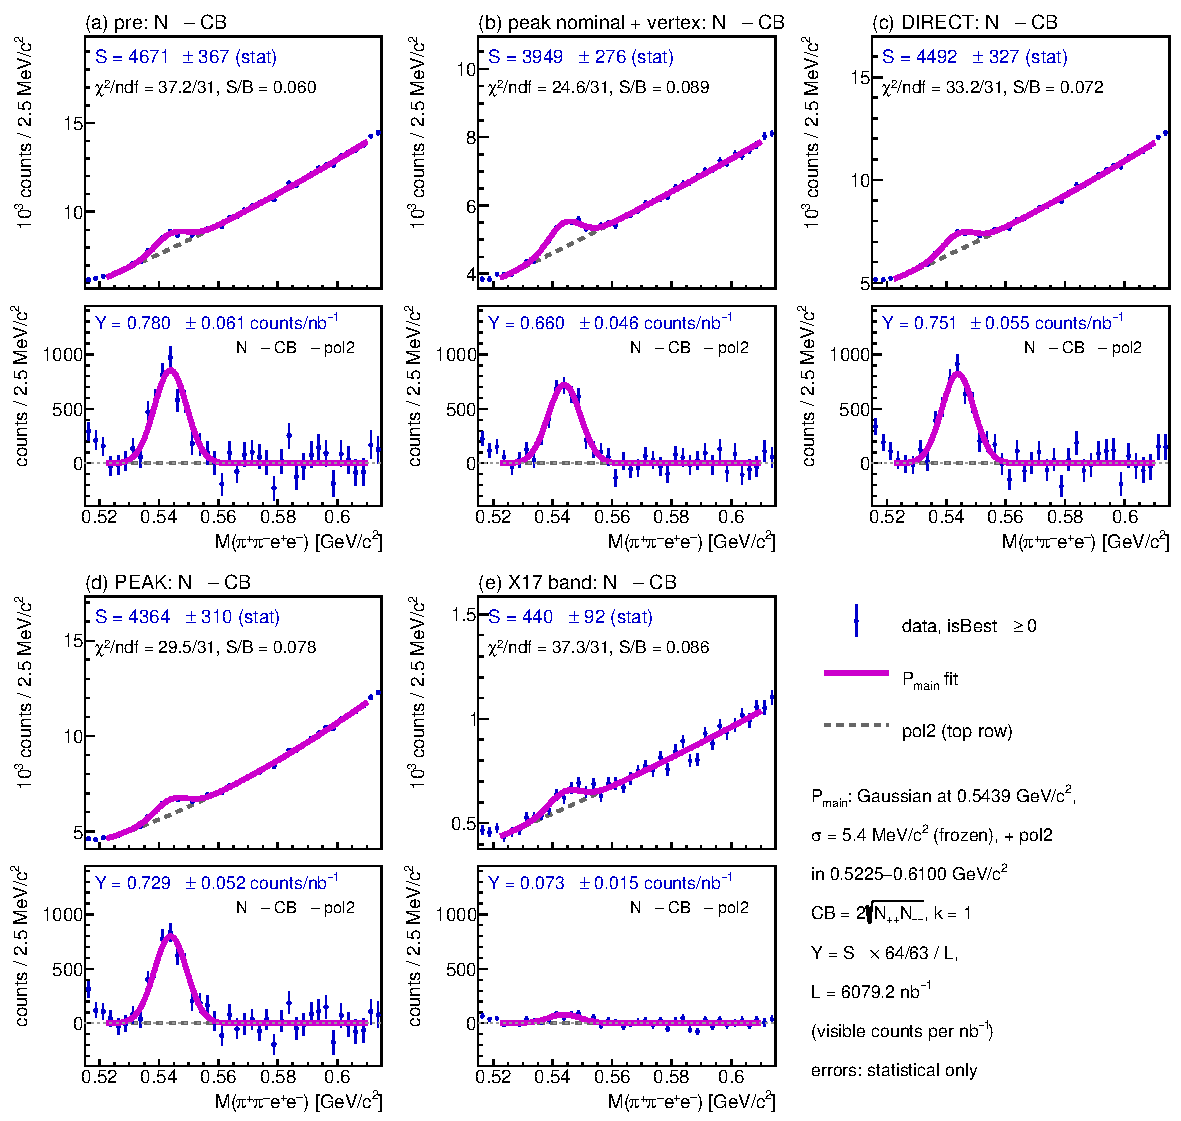
\includegraphics[width=\textwidth,trim=0 0 0 268,clip]{figs_exp/res_peak_fits_cnt.pdf}\\[0.3em]
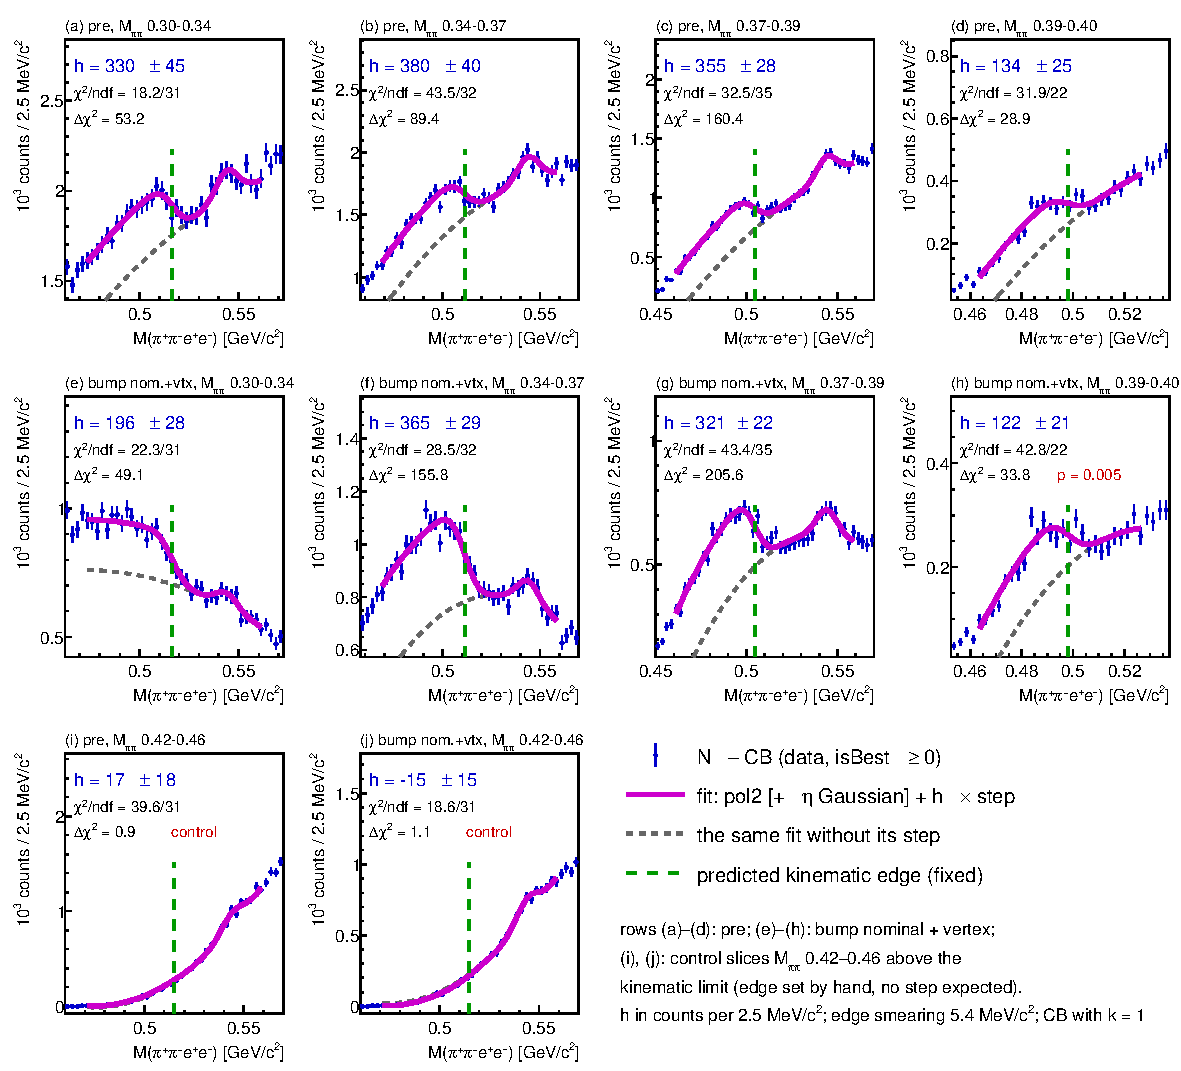
\includegraphics[width=\textwidth,trim=0 342 0 0,clip]{figs_exp/res_bump_slices_cnt.pdf}
\caption{\textbf{What it shows: the $\eta$ peak (top) and the bump edge (bottom) stand out.}
Both $\eta$ signals stand out in the data: the peak sits at the $\eta$ mass, the bump shows as an edge step. Selection: data; in every panel the base cuts: \ptthreecap{}, event vertex in the target region ($\vz>-160$\,mm), particles identified by their START-free velocity \betanew (pions within $3\sigma$, leptons within $5\sigma$ of their band; leptons with a RICH ring, pions without), energy-loss-corrected momenta of all four tracks (\code{cor_ok} $=1$), all stored \ppee combinations of each event (isBest $\ge0$) (``pre''). \emph{Top:} (d) PEAK $=$ ``pre'' + both pion tracks within 40\,mm of the event vertex along the beam ($\dzpi<40$\,mm) + missing mass of \ppee below 2.85\,\GeVcc ($\MMfour<2.85$\,\GeVcc); (e) X17 band $=$ ``pre'' + both pions used in the event-vertex fit + $15.5\le\Mee<24.5$\,\MeVcc, no \Mfour window; both fitted in 0.5225--0.6100\,\GeVcc with a fixed Gaussian (0.5439\,\GeVcc, width 5.4\,\MeVcc) plus a second-order polynomial. \emph{Bottom:} ``pre'' only ($=$ BUMP), all \Mee, in the four \Mpipi slices 0.30--0.34, 0.34--0.37, 0.37--0.39 and 0.39--0.40\,\GeVcc. CB in all panels: $2\sqrt{N_{++}N_{--}}$ from the like-sign counts (\pipi$e^+e^+$, \pipi$e^-e^-$) with the same cuts, in 10\,\MeVcc bins of \Mfour, $k=1$. \emph{Top, the peak}
(panels (d) and (e) of Fig.~\ref{fig:res_fits}): (d) PEAK (recommended), (e) X17 band, with the key; upper panels
$N-\mathrm{CB}$ with the \Pmain fit (magenta) and its polynomial (grey dashed), lower panels $N-\mathrm{CB}-\mathrm{pol2}$; statistical
errors only. \emph{Bottom, the bump edge} (panels (a)--(d) of Fig.~\ref{fig:res_slices}) in four \Mpipi slices of ``pre''
($=$ BUMP); blue $N-\mathrm{CB}$, magenta the fit with a step of height $h$ at the predicted kinematic edge (green dashed, fixed),
grey dashed the fit without the step. The bump measure is the sum of the four steps, $E=330+380+355+134=1199$ counts per
2.5\,\MeVcc. Counts (per 2.5\,\MeVcc), not normalised to luminosity except the printed $Y$.}
\label{fig:sum_signals}
\end{figure}

\paragraph{3. In the distance to the edge, the data show one sharp step.} \emph{What was done.} The edge of the bump is not one mass:
every count has its own, $\Medge(\Mpipi,\Mee)$, the largest \Mfour that $\eta\to\pipi\piz$, $\piz\to\ee\gamma$ with a lost photon can give for the
measured pion-pair and lepton-pair masses (Eq.~(\ref{eq:edgeu}); a heavier \ee pair leaves less energy to the photon and moves the edge up).
The distance to it, $u=\Mfour-\Medge$, is pure kinematics, so it needs no simulation. For a bump count $u\le0$ up to the resolution, whatever its
\Mpipi and \Mee: in $u$ the edges of all counts lie on top of each other at $u=0$, and one fit replaces the four slice fits of $E$.
\emph{Result} (``pre'' + both pions in the vertex fit, $0.30\le\Mpipi<0.40$\,\GeVcc, Fig.~\ref{fig:res-edgeu}): a fit of $N-\mathrm{CB}$ with
a second-order polynomial and a smeared step at $u=0$ on $-45\le u<+45$\,\MeVcc gives a step of $h_u=1308\pm62$ counts per 2.5\,\MeVcc;
without the step the fit is worse by $\Delta\chi^2=439$ (21$\sigma$), with it $\chi^2/\mathrm{ndf}=40.2/32$. A bootstrap of the data
confirms the error (63 counts). With its width left free the step is $6.3\pm0.7$\,\MeVcc wide, as expected from the mass resolution, and
$h_u=1271\pm85$. \emph{What was expected:} a step at $u=0$ and nowhere else; a control region above the kinematic limit
($0.42\le\Mpipi<0.46$\,\GeVcc, with a pseudo edge) shows none ($3.1\pm16.7$ counts, Part~III). \emph{One limit of a fit without the
simulation:} the $\eta$ peak begins at $u\approx+15$\,\MeVcc; without a peak term the polynomial absorbs the rise into the peak, and the step
height then depends on the fit range (1151 to 1477 counts); a peak term built from the data (the Gaussian of the data peak placed with the
measured \Mpipi and \Mee of the peak counts) gives $1217\pm66$ ($\chi^2/\mathrm{ndf}=24.6/31$, stable within 1205--1235 for other ranges), and
Part~III, with the simulated peak shape (which also has a low-mass tail), gets $1305\pm62$ ($\chi^2/\mathrm{ndf}=27.3/32$). \emph{Meaning:}
the data alone show the edge of $\eta\to\pipi\piz$ as one sharp step exactly where the kinematics of every count puts it; its height is fixed
to within about 7\,\%, depending on how the tail of the peak is modelled. \emph{Later (Part~III, checked by an independent verifier):} the
tail of the simulated peak is the radiation of the leptons in the detector material; of the 88 counts between 1305 and 1217 about 50 come from
leaving this tail out and about 40 from where the data put the peak counts; the data cannot measure the size of the tail ($0.3\pm1.0$ times the
simulated one), so the 7\,\% stay a modelling question (Part~III takes half of the simulated tail as a systematic term, D40, approved).
Like $E$, $h_u$ is a visibility measure, not a yield. Part~III turns this step into its bump measurement ($0.426$ of SMASH; D37 and D38,
approved; \S\ref{sec:needsim}). \emph{Reliability:}
measured; the step and its height in the data were found in Part~III (package edgeu) and confirmed by an independent verifier with own code;
the fit here is the same code without any simulated input (\S\ref{sec:edgeu}). Figure: Fig.~\ref{fig:res-edgeu}; details: \S\ref{sec:edgeu}.

\begin{figure}[!tbp]
\centering
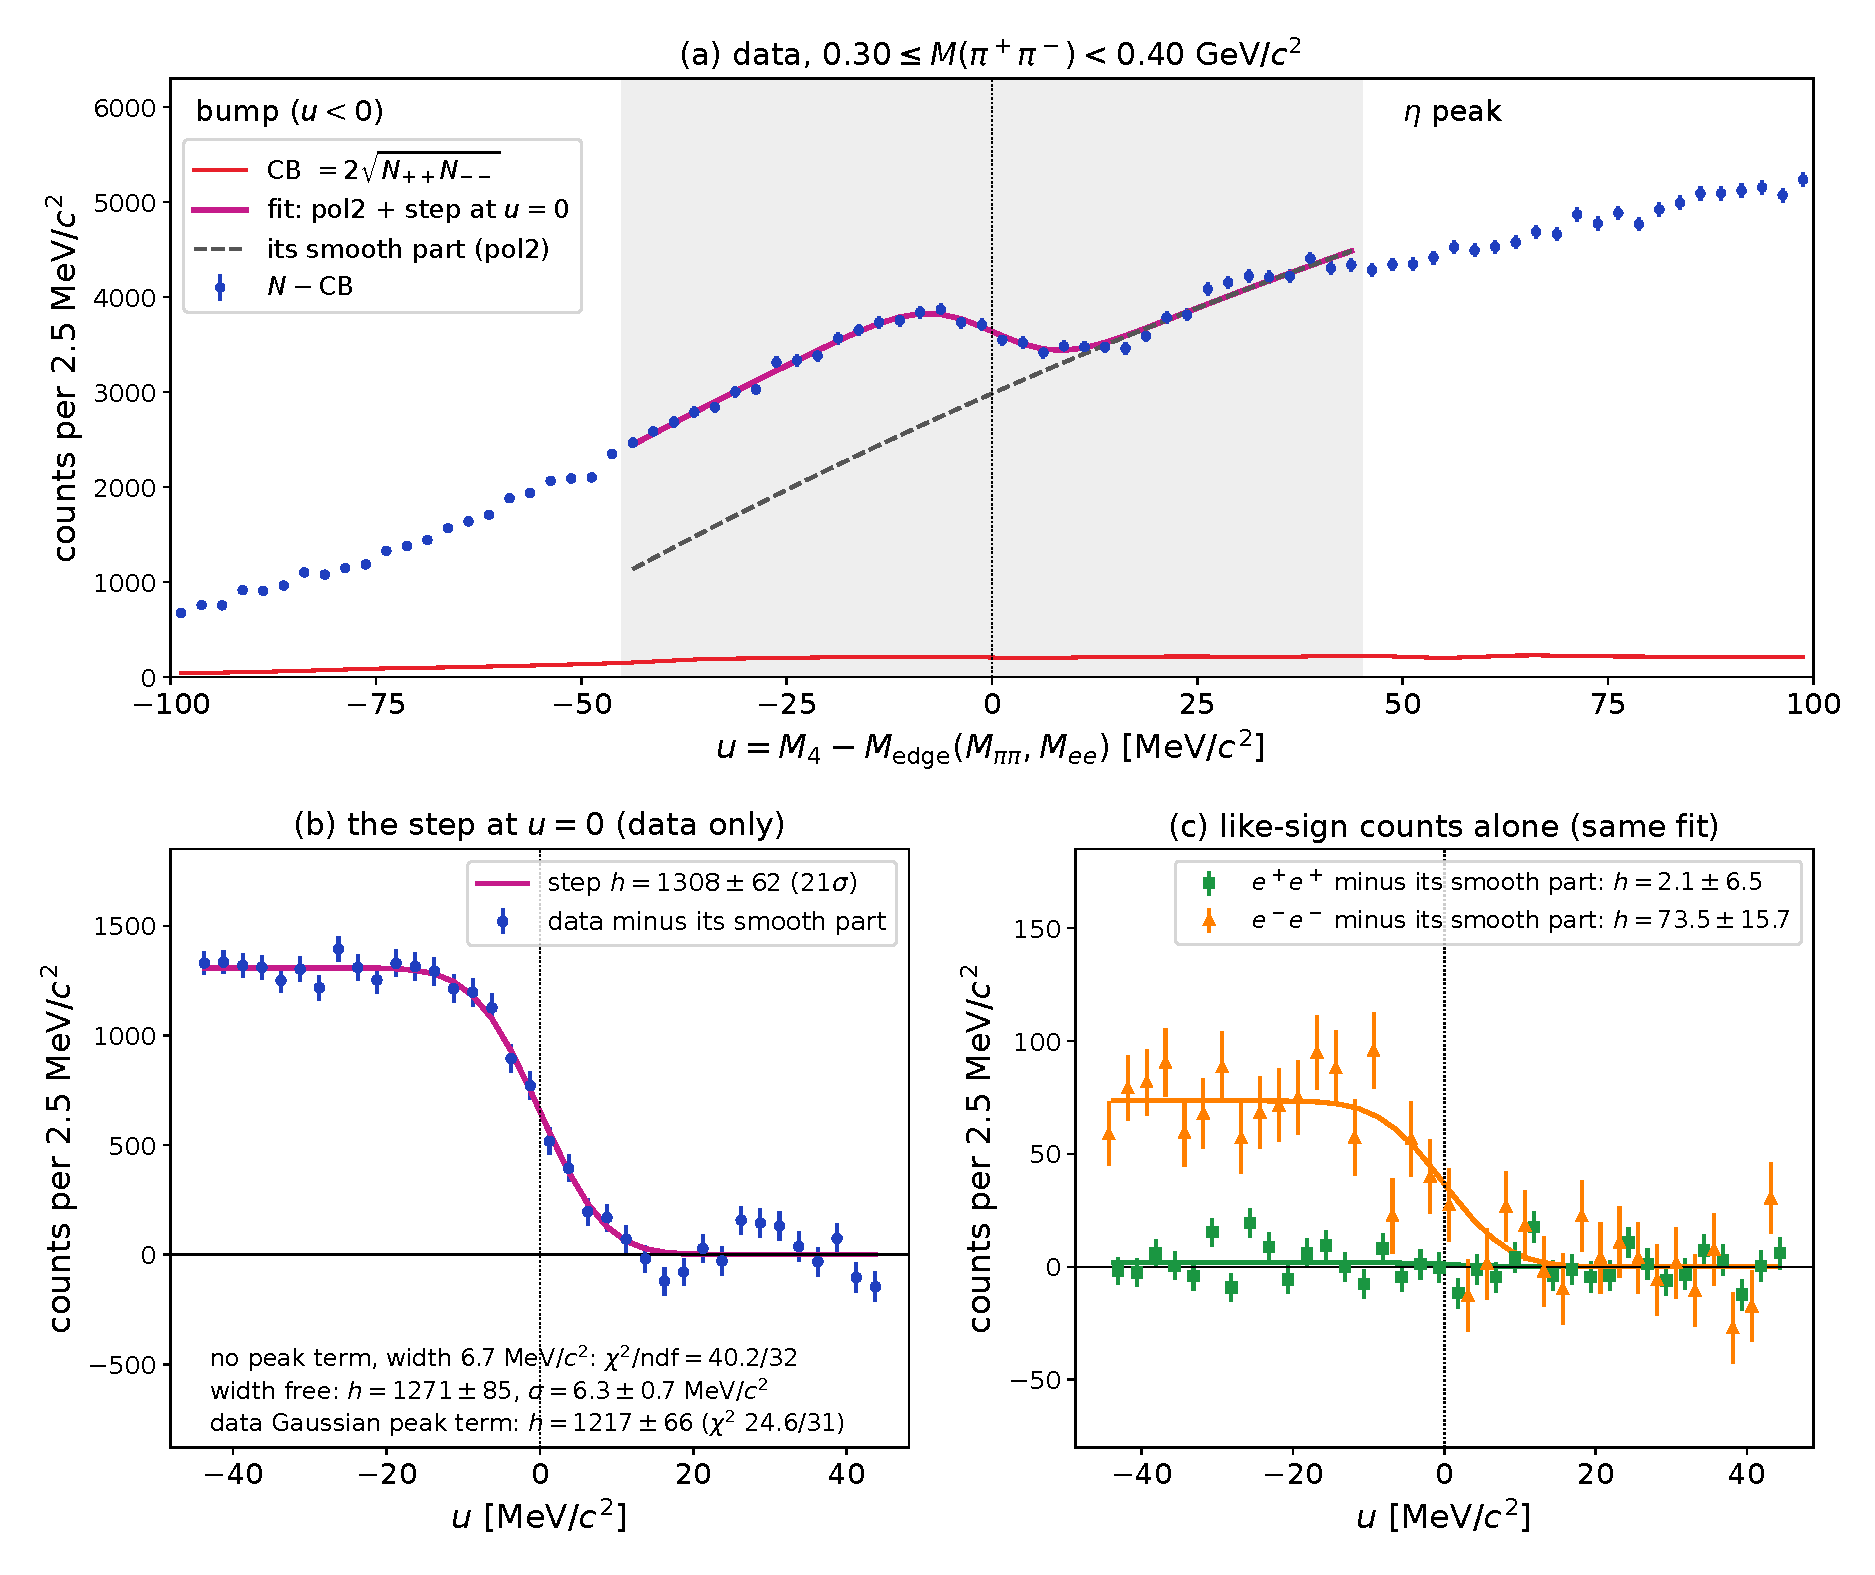
\includegraphics[width=0.92\textwidth]{figs_exp/p12w_edgeu_data_step_cnt.pdf}
\caption{\textbf{What it shows: in the distance to its edge, $u$, the bump is one sharp step at $u=0$; the like-sign counts step only a
little, almost all of it in $e^-e^-$ (pairs from the two \piz photons, at large \Mee).} Selection: data only; \ptthreecap{}, event vertex in the target region ($\vz>-160$\,mm), particles identified by their START-free velocity \betanew (pions within $3\sigma$, leptons within $5\sigma$ of their band; leptons with a RICH ring, pions without), energy-loss-corrected momenta of all four tracks (\code{cor_ok} $=1$), all stored \ppee combinations of each event (isBest $\ge0$), and both pions used in the event-vertex fit (``pre'' + vertex, Part~III's S0); $0.30\le\Mpipi<0.40$\,\GeVcc; $\Mee<m_{\pi^0}$ (135\,\MeVcc; above it $u$ is not defined); $-45\le u<+45$\,\MeVcc in 2.5\,\MeVcc bins; CB $=2\sqrt{N_{++}N_{--}}$ from the like-sign counts with the same cuts, in 10\,\MeVcc cells of $u$, separately in the \Mpipi slices 0.30--0.34, 0.34--0.37, 0.37--0.39 and 0.39--0.40\,\GeVcc, $k=1$; (c) the like-sign counts of the same selection.
$u=\Mfour-\Medge(\Mpipi,\Mee)$ with the edge of Eq.~(\ref{eq:edgeu}) on the data mass scale. (a, top) $N-\mathrm{CB}$ (blue), CB
$=2\sqrt{N_{++}N_{--}}$ in 10\,\MeVcc cells of $u$ per \Mpipi slice (red), the fit with a second-order polynomial and a step at $u=0$
smeared with 6.7\,\MeVcc (magenta) on $-45\le u<+45$\,\MeVcc (grey band) and its smooth part (dashed); the bump lies at $u<0$, the $\eta$
peak at $u\approx+20$ to $+55$\,\MeVcc. (b, bottom left) The data minus the smooth part: the step, $h_u=1308\pm62$ counts (21$\sigma$); printed: the fit
quality, the result with the width left free and with a Gaussian peak term built from the data. (c, bottom right) The like-sign counts alone with the
same fit: $e^+e^+$ (green) $2.1\pm6.5$, $e^-e^-$ (orange) $73.5\pm15.7$ counts (4.7$\sigma$; lepton pairs from the two \piz photons at large \Mee, Fig.~\ref{fig:res-eestep},
\S\ref{sec:cbnull}, D39). Counts per
2.5\,\MeVcc, not normalised to luminosity. Macro \code{plots/all_report/edgeu_partII_datastep.py} (axis label \Medge: \code{p12w_partII_figs.py}).}
\label{fig:res-edgeu}
\end{figure}

\paragraph{4. A third $\eta$ signal: the ECAL-tagged $\eta\to\pipi\piz$.} When the electromagnetic calorimeter (ECAL) also finds the photon, the full
decay $\eta\to\pipi\piz$ appears as a peak: $T=3314\pm105\pm124$ counts for ``pre'' ($Y_T=0.554\pm0.018$ visible counts per \nbinv); the
peak over the tagged content is $S/T=1.409\pm0.119\pm0.15$, not corrected for the different acceptances. \emph{Meaning:} a third,
clean $\eta$ signal and the reference of the vertex and period checks. \emph{Reliability:} final; the tagged $\eta$ serves for
verification only (the ECAL energy is not calibrated, but the photon energy is rescaled combination by combination, so $T$ is not affected). \emph{Later
(Part~III, data side):} the ECAL module map of the data is the same in all four periods and the same as in the simulation: ECAL
sector~0 (azimuth 63--117$^\circ$) is switched off and 8 further modules are dead, and the tagged photons of the data leave ECAL sector~0
empty. The photon cut $0.8<\beta<1.2$ uses the START time: the 6.4\,\% of the \ee counts without a START hit are tagged at only 0.69--0.80 of
the normal rate, which costs $T$ 1.4--2.3\,\%. The photon energy of the data is about 17\,\% too high (the median factor that brings
$M(\ee\gamma)$ of the tagged counts to the \piz mass is 0.856), so the 100\,MeV cluster cut acts near 85\,MeV of true photon energy. None of this changes $T$; it matters only when $T$ is compared with a simulated tag (Part~III).
Figure: Fig.~\ref{fig:res-tagged}; details: \S\ref{sec:tagged}.

\begin{figure}[!tbp]
\centering
% Section-1 copy of Fig. res_tagged (Section 7), placed next to its result
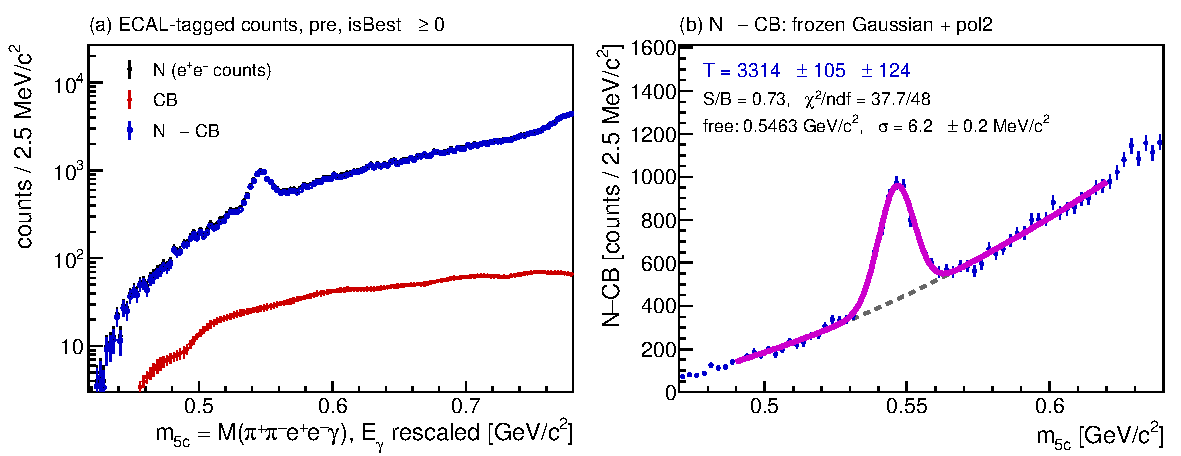
\includegraphics[width=\textwidth]{figs_exp/res_bump_tagged_cnt.pdf}
\caption{\textbf{What it shows: with the ECAL photon, $\eta\to\pipi\piz$ gives a clean third $\eta$ peak.}
When the ECAL also finds the photon, the full decay appears as a peak. Selection: data; \ptthreecap{}, event vertex in the target region ($\vz>-160$\,mm), particles identified by their START-free velocity \betanew (pions within $3\sigma$, leptons within $5\sigma$ of their band; leptons with a RICH ring, pions without), energy-loss-corrected momenta of all four tracks (\code{cor_ok} $=1$), all stored \ppee combinations of each event (isBest $\ge0$) (``pre''); in addition a good ECAL photon (identified as a photon by the ECAL, $0.8<\beta<1.2$, cluster energy above 100\,MeV; of up to three such photons the one with $M(\ee\gamma)$ closest to 0.140\,\GeVcc) with $0.119\le M(\ee\gamma)<0.173$\,\GeVcc, and $\Mee<0.10$\,\GeVcc; $m_{5c}$ in 2.5\,\MeVcc bins, fit range 0.49--0.62\,\GeVcc; CB $=2\sqrt{N_{++}N_{--}}$ from the like-sign counts with the same cuts, in 20\,\MeVcc bins, $k=1$. The same figure as Fig.~\ref{fig:res_tagged} (\S\ref{sec:tagged}). X axis $m_{5c}=M(\ppee\gamma)$ with the photon energy rescaled so
that $M(\ee\gamma)=m_{\pi^0}$. (a) $N$ black, CB red ($k=1$), $N-\mathrm{CB}$ blue open; log scale. (b) $N-\mathrm{CB}$ with the frozen
Gaussian (0.5463\,\GeVcc, 6.2\,\MeVcc) + pol2 fit: $T=3314\pm105\,(\mathrm{stat})\pm124\,(\mathrm{model})$ counts, $Y_T=0.554\pm0.018$ visible
counts per \nbinv. Counts, not normalised to luminosity except the quoted $Y_T$.}
\label{fig:res-tagged}
\end{figure}

\paragraph{5. The combinatorial background is small, and the $\eta$ results hardly depend on it.} The CB (counts whose $e^+$ and $e^-$
come from two different sources) is estimated from the like-sign counts of the same events as $2\sqrt{N_{++}N_{--}}$. In the peak
window it is 0.103 of the counts for ``pre'', 0.072 for PEAK and 0.019 in the X17 band; most of the background under the peaks is made
of true \ee pairs with pions (``physical'' background), which the polynomial of the fit describes. The like-sign counts show no $\eta$
peak and no bump edge in \Mfour (Fig.~\ref{fig:res-cb}, bottom); in the distance to the edge, $u$, the $e^-e^-$ counts do show a small step
(paragraph~6). A CB change of $\pm3$\,\% moves $S$ by at most 0.07\,\% and $E$ by 0.1\,\%; even a 38--45\,\% larger CB (the
plain sum $N_{++}+N_{--}$) moves $S$ by at most 1\,\% and $E$ by 3\,\%. \emph{Reliability:} shares, null tests and sensitivities are
final; the convention $k=1$ is provisional (event mixing gives 1.01--1.04); the absolute normalisation of the CB is \textbf{not
determined}: the like-sign counts hold 5.4 times more $e^-e^-$ than $e^+e^+$ (1.17 expected for independent leptons), a correlated
source that event mixing cannot see, so CB$/N$ and window counts carry an unknown scale. Figure: Fig.~\ref{fig:res-cb}; details: \S\ref{sec:spec},
\S\ref{sec:cbnull}.

\begin{figure}[!tbp]
\centering
% Section-1 copy: res_peak_overview (Section 7), panel (a) of cb_sensitivity (Section 5) and the null tests cb_null (Section 5.5)
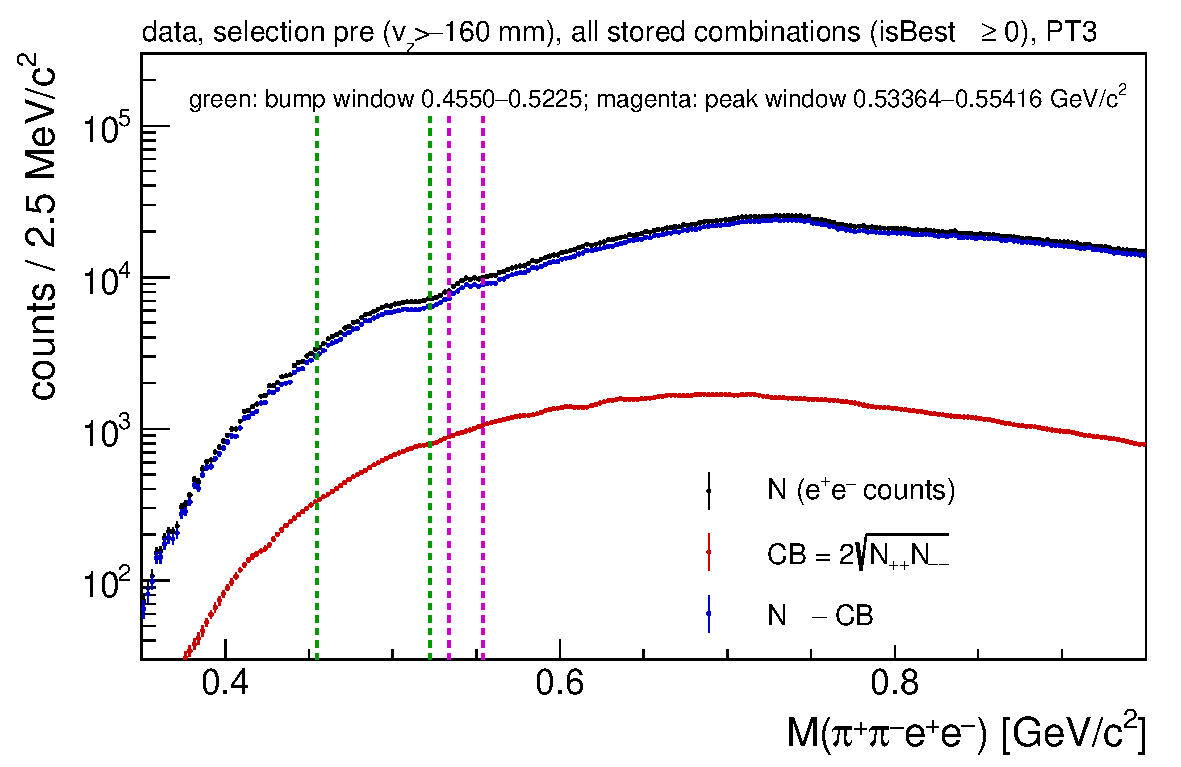
\includegraphics[height=0.378\textwidth]{figs_exp/res_peak_overview_cnt.pdf}\hfill
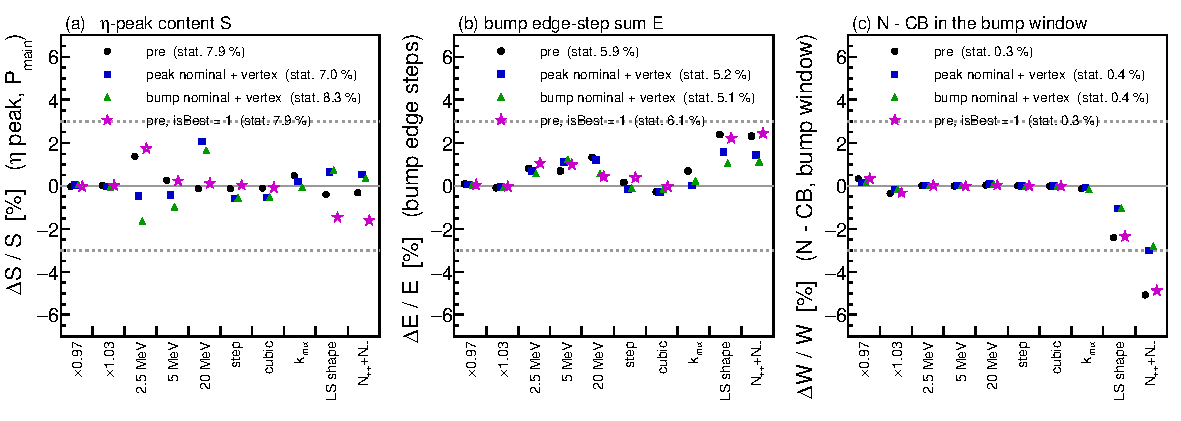
\includegraphics[height=0.378\textwidth,trim=0 0 378 0,clip]{figs_exp/cb_sensitivity.pdf}\\[0.3em]
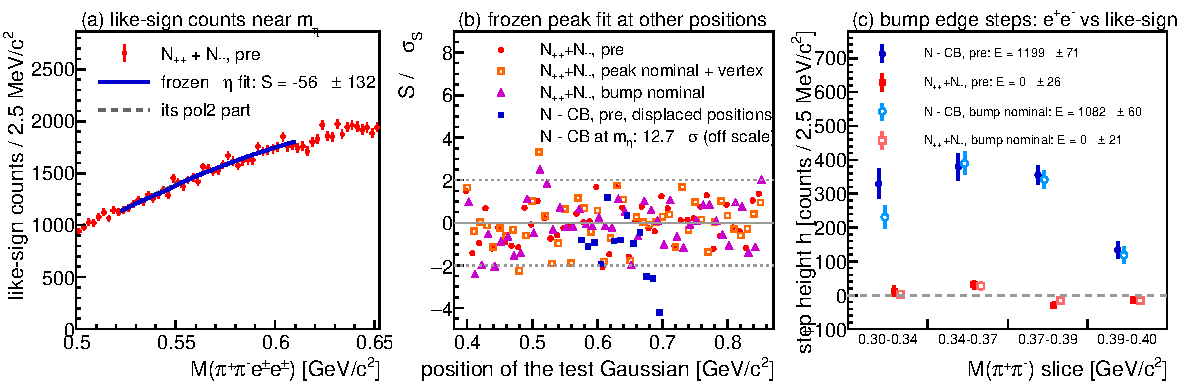
\includegraphics[width=0.91\textwidth]{figs_exp/cb_null_cnt.pdf}
\caption{\textbf{What it shows: the CB is small, shows no $\eta$ signal and barely moves $S$.}
The CB is a small part of the spectrum (top left, red), and changing it hardly moves the $\eta$-peak content (top right); the like-sign
counts from which it is built show no $\eta$ peak and no bump edge in \Mfour (bottom; the $e^-e^-$ step in $u$ is described in
\S\ref{sec:cbnull} and shown in Fig.~\ref{fig:res-edgeu}c). Selection: data; every panel starts from the base cuts: \ptthreecap{}, event vertex in the target region ($\vz>-160$\,mm), particles identified by their START-free velocity \betanew (pions within $3\sigma$, leptons within $5\sigma$ of their band; leptons with a RICH ring, pions without), energy-loss-corrected momenta of all four tracks (\code{cor_ok} $=1$), all stored \ppee combinations of each event (isBest $\ge0$) (``pre''). Top left: ``pre'' only. Top right: ``pre''; peak nominal + vertex $=$ ``pre'' + the angle between the \pipi and \ee momenta in the laboratory below $55^\circ$ ($\alab<55^\circ$), $\Mpipi>0.30$\,\GeVcc and both pions used in the event-vertex fit; bump nominal + vertex $=$ ``pre'' + $\alab<40^\circ$, $0.30<\Mpipi<0.41$\,\GeVcc and both pions used in the event-vertex fit; ``pre'' with only the best-ranked combination of each event (isBest $=1$). Bottom: (a) ``pre''; (b) ``pre'', peak nominal + vertex and bump nominal ($\alab<40^\circ$, $0.30<\Mpipi<0.41$\,\GeVcc, no vertex-fit requirement), the $N-\mathrm{CB}$ points ``pre'' only; (c) ``pre'' and bump nominal, in the four \Mpipi slices 0.30--0.34, 0.34--0.37, 0.37--0.39 and 0.39--0.40\,\GeVcc. CB $=2\sqrt{N_{++}N_{--}}$ from the like-sign counts (\pipi$e^+e^+$, \pipi$e^-e^-$) with the same cuts, in 10\,\MeVcc bins of \Mfour, $k=1$ (top right: also the variants listed below).
Top left, the same as Fig.~\ref{fig:res_overview}: \Mfour of ``pre'', all combinations (isBest $\ge0$); black $N$, red CB $=2\sqrt{N_{++}N_{--}}$
($k=1$), blue $N-\mathrm{CB}$; 2.5\,\MeVcc bins, log scale; green lines: bump window 0.4550--0.5225\,\GeVcc; magenta lines: peak window
0.53364--0.55416\,\GeVcc, where CB$/N$ is 0.103 (0.072 for PEAK). Top right, panel (a) of Fig.~\ref{fig:cb_sensitivity}: change of $S$ (\Pmain)
in per cent when the CB estimate is changed, for ``pre'', peak nominal + vertex, bump nominal + vertex (isBest $\ge0$) and ``pre'' with
isBest $=1$ (legend: statistical error of $S$). Variants: CB$\times0.97$ and $\times1.03$ (at most 0.07\,\%); CB bins of 2.5, 5,
20\,\MeVcc ($-1.6$\dots$+2.1$\,\%, mostly the statistical noise of the CB estimate); step and cubic interpolation; CB$\times
k_{\mathrm{mix}}$; the like-sign sum shape; the plain sum $N_{++}+N_{--}$, a CB larger by 38--45\,\% (at most 1\,\%; isBest $=1$ and the
X17 band up to 2.3\,\%). Dotted: $\pm3$\,\%. Bottom, the same as Fig.~\ref{fig:cb_null} (\S\ref{sec:cbnull}): null tests of the
like-sign counts, isBest $\ge0$. (a) $N_{++}+N_{--}$ near $m_\eta$, ``pre'', with the frozen $\eta$ fit: $S=-56\pm132$, while $N-\mathrm{CB}$ gives
$4671\pm367$. (b) $S/\sigma_S$ of the same fit moved with its range: $N_{++}+N_{--}$ at 46 positions 0.40--0.85\,\GeVcc, $N-\mathrm{CB}$ at 13
positions 0.575--0.695\,\GeVcc (blue squares). (c) Bump edge-step heights per \Mpipi slice on $N-\mathrm{CB}$ (blue) and on $N_{++}+N_{--}$
with the same fixed edges (red), for ``pre'' and bump nominal; counts per 2.5\,\MeVcc. Counts, not normalised to luminosity.}
\label{fig:res-cb}
\end{figure}

\paragraph{6. In the distance to the edge, the $e^-e^-$ like-sign counts show a step: lepton pairs from the two \piz photons (explained).}
\emph{What was found.} The same fit as in paragraph~3, applied to the like-sign counts alone, gives a step of $73.5\pm15.7$ counts per
2.5\,\MeVcc (4.7$\sigma$) for $e^-e^-$ and $2.1\pm6.5$ for $e^+e^+$ (Fig.~\ref{fig:res-edgeu}c). \emph{What was expected:} no step, if the
like-sign pairs were made only of leptons from unrelated sources. \emph{What it is.} A dedicated study (Part~III, package eestep; its data side
is given here) found that the step counts are pairs of leptons from the \emph{two different photons} of the \piz in $\eta\to\pipi\piz$: a Dalitz
$e^-$ and a conversion $e^-$ of the other photon, or two conversion $e^-$. Kinematics gives such pairs exactly the edge of the bump at the
same \Mee, and near the edge they are heavy. The data show just that (Fig.~\ref{fig:res-eestep}): the $e^-e^-$ step lies at
\Mee$\ge90$\,\MeVcc ($57.0\pm9.1$ counts, 6.3$\sigma$) and is absent below 50\,\MeVcc ($3.6\pm8.9$), where 90\,\% of the bump lies; the two
$e^-$ are 20--60$^\circ$ apart; the step follows the edge with its \Mee term ($\Delta\chi^2=28.3$, against 0.5 with the edge at
$\Mee\to0$), which is why \Mfour per slice (paragraph~5, $0.5\pm25.6$) sees no like-sign step; 85\,\% of these counts come from events with no
positive lepton at all; the $e^+e^+$ counts show the same step at \Mee$\ge90$\,\MeVcc, smaller ($7.3\pm4.3$ counts, ratio $0.13\pm0.08$), because
soft $e^+$ are accepted less often than soft $e^-$, and because a photon can also give a Compton or knock-on electron, which is always
negative (SMASH contains such pairs, mostly $e^-e^-$). It is \emph{not} a Dalitz $e^+$ reconstructed with a negative charge: such a count keeps the
small \Mee of the bump, where there is no step (charge-flip rate $<1.2$\,\%, 90\,\% CL). \emph{Meaning for the data.} A decay with a Dalitz or
conversion pair on each photon also gives two $e^+e^-$ cross pairs in $N$ (a Compton or knock-on electron gives one), and CB $=2\sqrt{N_{++}N_{--}}$
is built to subtract them. Where the bump is small (\Mee$\ge90$\,\MeVcc) the
unlike-sign counts indeed carry the matching step: $N$ $52.6\pm10.9$ counts, CB $35.8\pm8.6$, $N-\mathrm{CB}=16.8\pm13.9$ (Part~III: the bump
signal expected there, SMASH $\times f$ with the per-count C2 weights of D38, is 16.9 counts; a like-sign artefact without partners would
leave $-19.0$, 2.6$\sigma$ away, statistical; about 2.3$\sigma$ with the error of the simulated prediction, $\pm6.7$). So the CB treats the step as
designed: the 39 counts (3\,\% of $h_u$) it carries belong there. The $\eta$ peak is not affected (cross pairs reach the peak window only at
\Mee$\ge102$--120\,\MeVcc and are subtracted with their partners), nor is the X17 band. The earlier caveat ``the bump scale of Part~III could
be up to about 8\,\% higher'' is withdrawn (Part~III: at most $+1.6$\,\% from an $e^+\to e^-$ flip, 1.9\,\% for a flip of either charge).
\emph{Reliability:} measured; mechanism found by the lead analysis and confirmed by an independent verifier with own code (only the wording
was corrected; its toy also predicts the step position, $-2.5$\,\MeVcc, that the data show); recorded as D39 (origin recorded, CB kept), approved by the analyst on 15 November 2026.
Figure: Fig.~\ref{fig:res-eestep}; details: \S\ref{sec:cbnull}.

\begin{figure}[!tb]
\centering
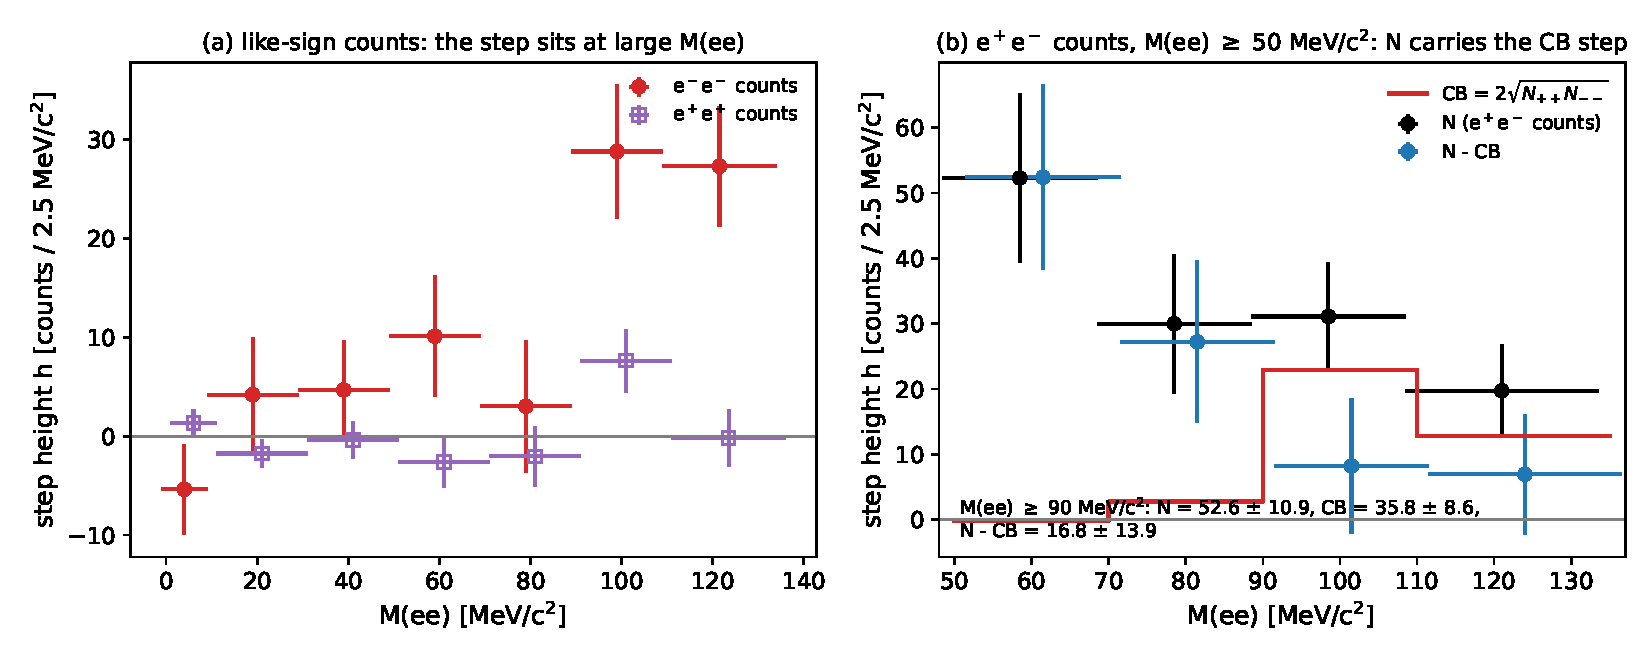
\includegraphics[width=\textwidth]{figs_exp/eestep_bands_data_cnt.pdf}
\caption{\textbf{What it shows: the like-sign step at the bump edge sits at large \Mee, where lepton pairs from the two \piz photons lie, and
there the unlike-sign counts carry the matching step, which the CB subtracts.} Selection: data only; \ptthreecap{}, event vertex in the target region ($\vz>-160$\,mm), particles identified by their START-free velocity \betanew (pions within $3\sigma$, leptons within $5\sigma$ of their band; leptons with a RICH ring, pions without), energy-loss-corrected momenta of all four tracks (\code{cor_ok} $=1$), all stored \ppee combinations of each event (isBest $\ge0$), and both pions used in the event-vertex fit (``pre'' + vertex); $0.30\le\Mpipi<0.40$\,\GeVcc; the step fit of Fig.~\ref{fig:res-edgeu} ($-45\le u<+45$\,\MeVcc, second-order polynomial plus a step at $u=0$ smeared with 6.7\,\MeVcc) done separately in the \Mee bands 0--10, 10--30, 30--50, 50--70, 70--90, 90--110 and 110--135\,\MeVcc ((b): the bands from 50\,\MeVcc up); CB of each band from the like-sign counts of that band, $k=1$.
Step height $h$ at $u=0$ (counts per 2.5\,\MeVcc) of the fit of
Fig.~\ref{fig:res-edgeu}, per \Mee band. (a) Like-sign counts: $e^-e^-$ (red points), $e^+e^+$ (violet open squares); no step below
50\,\MeVcc, a step at \Mee$\ge90$\,\MeVcc in both. (b) Unlike-sign counts at \Mee$\ge50$\,\MeVcc: $N$ (black), the CB of each band from its own
like-sign counts (red line) and $N-\mathrm{CB}$ (blue). Counts, not normalised to luminosity. Macro
\code{plots/all_report/eestep_partII_fig.py} (numbers of package eestep).}
\label{fig:res-eestep}
\end{figure}

\paragraph{7. The selection frozen on the simulation is as good as the best one tuned on the data.} Cuts chosen on the same data on
which they are measured favour upward fluctuations; this bias was measured on independent halves of the data. PEAK, chosen blind on
the simulation in Part~I (``pre'' + both pion tracks within 40\,mm in $z$ of the event vertex + missing mass below 2.85\,\GeVcc),
improves the precision $F=S/\mathrm{stat}$ over ``pre'' by $+1.35$, as much as the best blind procedure on the data ($+1.36$); the selection
optimised on these data (peak nominal + vertex) gains $+1.57$, but only about $+1.15$ after its bias is removed. The vertex cuts do
most of the work; a cut on the \ee opening angle (OA$>2^\circ$) keeps only 0.78 of the peak and never improves the precision. The PEAK cuts keep the same share of the
$\eta$ in the data as in the simulation within the data errors. \emph{Reliability:} provisional, a recommendation open for review (decision (i));
the missing-mass cut may create a small fake peak content, $+48\pm27$ or $+83\pm26$ counts ($\le1.9$\,\% of $S$, one-sided; two
implementations disagree). Figure: Fig.~\ref{fig:res-selection}; details: \S\ref{sec:opt}, \S\ref{sec:recommend}.

\begin{figure}[!tbp]
\centering
% Section-1 copy of Fig. opt_bias (Section 6)
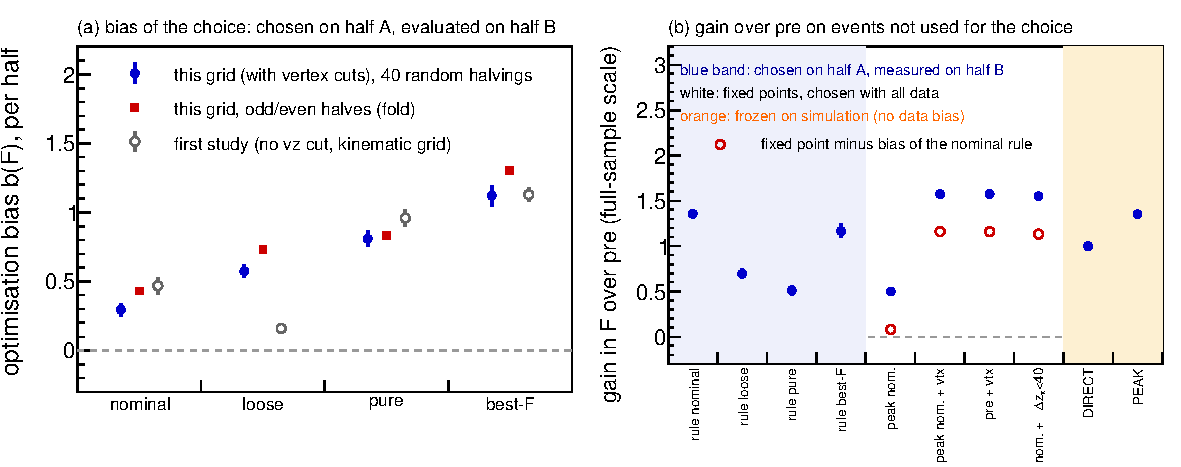
\includegraphics[width=\textwidth]{figs_exp/opt_bias.pdf}
\caption{\textbf{What it shows: the frozen PEAK gains as much as the best data choice.}
PEAK, frozen on the simulation, gains as much precision as the best blind choice on the data (right). Selection: data; every selection starts from the base cuts: \ptthreecap{}, event vertex in the target region ($\vz>-160$\,mm), particles identified by their START-free velocity \betanew (pions within $3\sigma$, leptons within $5\sigma$ of their band; leptons with a RICH ring, pions without), energy-loss-corrected momenta of all four tracks (\code{cor_ok} $=1$), all stored \ppee combinations of each event (isBest $\ge0$) (``pre''); $S$ from a fit of $N-\mathrm{CB}$ in 0.5225--0.6100\,\GeVcc with a fixed Gaussian (0.5439\,\GeVcc, width 5.4\,\MeVcc) plus a second-order polynomial (\Pmain). Blind rules: working points chosen from a grid of 840 cut combinations on top of ``pre'': the angle between the \pipi and \ee momenta in the laboratory ($\alab$) below 40, 45, 50, 55, 60 or $65^\circ$ or no cut; $\Mpipi>0.34$, 0.32 or 0.30\,\GeVcc or no cut; both pions, at least one pion or no requirement in the event-vertex fit; $\dzpi<20$, 30, 40 or 60\,mm or no cut; $\MMfour<2.85$\,\GeVcc or no cut. Fixed points (white region): peak nominal ($\alab<55^\circ$, $\Mpipi>0.30$\,\GeVcc), peak nominal + both pions in the vertex fit, ``pre'' + both pions in the vertex fit, peak nominal + $\dzpi<40$\,mm. Frozen on the simulation (orange): PEAK (both pion tracks within 40\,mm of the event vertex along the beam ($\dzpi<40$\,mm), and a missing mass of \ppee below 2.85\,\GeVcc) and DIRECT ($\dzpi<40$\,mm only). Halves: event groups split at random (40 halvings) or by the parity of the group index; the first study (grey) used a kinematic grid without vertex cuts and without the $\vz$ cut. The same as Fig.~\ref{fig:opt_bias} (\S\ref{sec:bias}); data, isBest $\ge0$, \Pmain. (b), the key panel: gain in $F=S/\mathrm{stat}$ over
``pre'' on the events not used for the choice (full-sample scale): blind rules chosen on one half and measured on the other (blue band; the
nominal rule $+1.36$); fixed points chosen with all data (white region; peak nominal + vertex $+1.57$, open red: minus the bias of the
nominal rule, about $+1.15$); selections frozen on the simulation (orange band; PEAK $+1.35$, DIRECT $+1.00$). (a) Bias $b(F)$ per half of
four fixed rules choosing a working point on one half (grid of 840 points on top of ``pre''): 40 random halvings (blue), odd/even halves
(red), first study (grey). Counts, not normalised to luminosity.}
\label{fig:res-selection}
\end{figure}

\paragraph{8. The mandatory event-vertex cut keeps the $\eta$.} The production keeps only entries with a reconstructed event vertex
($\vz>-500$\,mm), which removes 32\,\% of the \ee counts. In the removed counts the tagged $\eta$ is $-4\pm77$ counts (3297 in the kept counts)
and the bump edge $21\pm96$ (1241): with three measures combined, the cut keeps $\varepsilon_{\mathrm{vtx}}=0.994\pm0.021$ of the
$\eta$ ($0.990\pm0.022$ with the nominal CB). Most of the removed counts do not come from p+p collisions in the hydrogen cell (87\,\% of their pion
pairs cross 8\,mm or more from the beam axis, against 35\,\% with a vertex); they probably come from beam halo on the material in front
of the cell (a hypothesis; the empty-target runs show that beam halo on material in front of the cell makes such counts at a large rate, \S\ref{sec:walls}). \emph{Meaning:} the cut is validated; the survival of the counts, 0.565 in the peak window, is not an $\eta$ efficiency; a correction
would raise the yields by $0.6\pm2.1$\,\% and is not applied. \emph{Reliability:} measured after the review, the decisive study by an
independent verifier with own code; the method choices are decision (ix). Figure: Fig.~\ref{fig:res-vertex}; details: \S\ref{sec:vtxeff}.

\begin{figure}[!tb]
\centering
% Section-1 copy: bottom row, panels (e) and (f), of fix2_vtx_fig (Section 7)
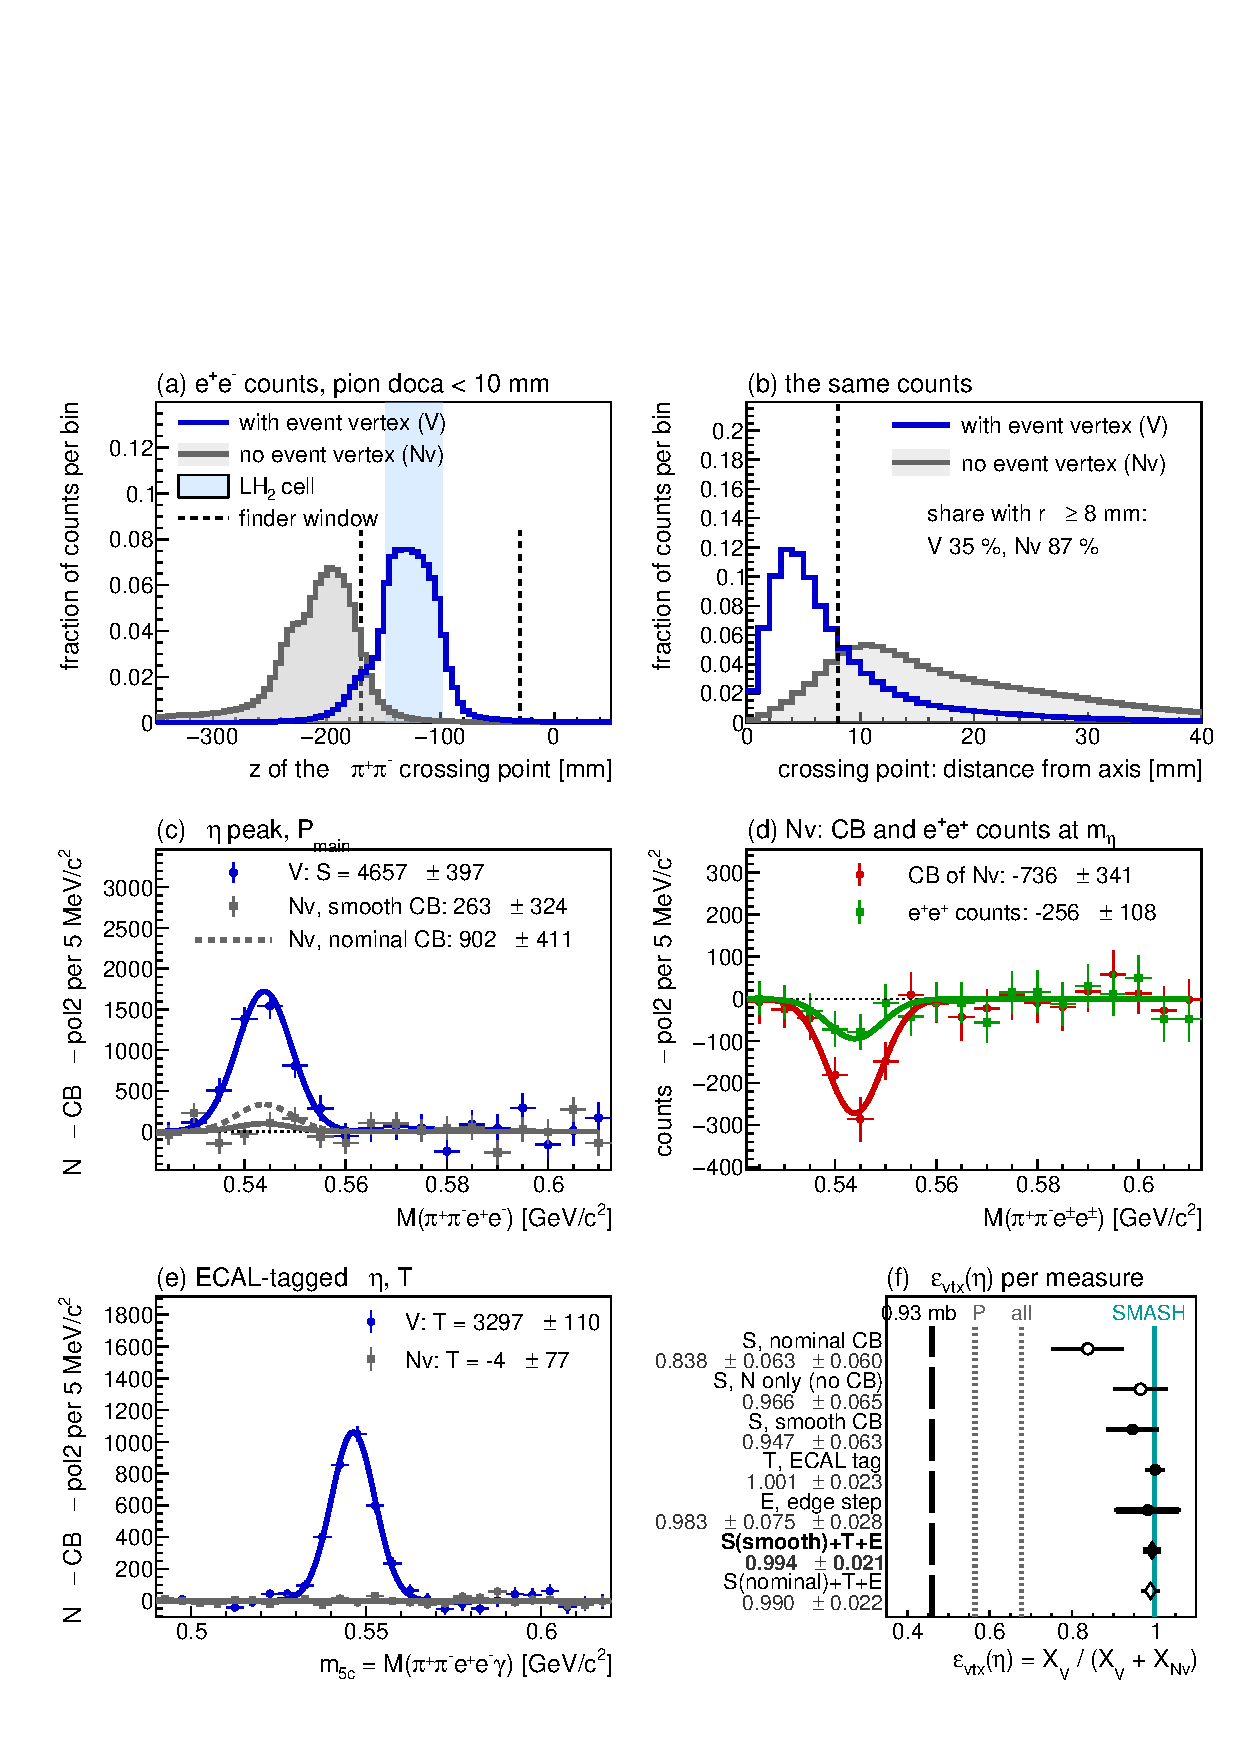
\includegraphics[width=0.92\textwidth,trim=0 0 0 432,clip]{figs_exp/fix2_vtx_fig_cnt.pdf}
\caption{\textbf{What it shows: the counts removed by the vertex cut hold no $\eta$.}
So the cut keeps the $\eta$: the counts removed by the event-vertex cut hold no tagged $\eta$ (left, grey), so the cut keeps the $\eta$ (right). Selection: data, all 29 PAT day files read directly (before FAT); \ptthreecap{}, the \betanew particle identification of PAT, energy-loss-corrected momenta of all four tracks (\code{cor_ok}), all stored combinations (isBest $\ge0$); no target-region cut and no pion-vertex requirement; whole events split into those with a reconstructed event vertex (V, $\vz>-500$\,mm) and those without (Nv, $\vz=-1000$\,mm), each with its own CB $=2\sqrt{N_{++}N_{--}}$ from its own like-sign counts, $k=1$. (e) in addition the ECAL photon of Fig.~\ref{fig:res-tagged} ($0.119\le M(\ee\gamma)<0.173$\,\GeVcc, $\Mee<0.10$\,\GeVcc). (f) the three measures on these counts: $S$ (fixed-Gaussian fit in 0.5225--0.6100\,\GeVcc), $T$ as in (e), $E$ (edge steps in the four \Mpipi slices 0.30--0.34, 0.34--0.37, 0.37--0.39 and 0.39--0.40\,\GeVcc). Panels (e) and (f) of Fig.~\ref{fig:vtxeff} (\S\ref{sec:vtxeff}). Counts with an
event vertex (V) blue, without (Nv) grey. (e) ECAL-tagged $\eta$ in $m_{5c}$, $N-\mathrm{CB}-$pol2 per 5\,\MeVcc: $T=3297\pm110$ (V) against
$-4\pm77$ (Nv). (f) $\varepsilon_{\mathrm{vtx}}=X_V/(X_V+X_{Nv})$ for each measure $X$ (open: not used for the result; $E$: thick bar stat
$\times1.2$, kept as a conservative choice, thin bar with the model rms); combined $S$ (smooth CB) $+$ $T$ $+$ $E$: $0.994\pm0.021$ ($0.990\pm0.022$ with the nominal CB);
lines: simulation 0.9997, survival of the counts 0.565 and 0.677, and 0.46, which 0.93\,mb would need in Part~III. Counts, not normalised to luminosity.}
\label{fig:res-vertex}
\end{figure}

\paragraph{9. Normalisation.} The luminosity of the analysed runs, from the START-free analysis of elastic p+p scattering, is
$\Lan=6079.2\,\nbinv\pm6.9$\,\%; the yields include the trigger-bit factor 64/63. Three one-sided effects that are not corrected in
the yields could make them up to about 11\,\% too low: the PT3/PT2 live fraction, if it applies (up to $+7.3$\,\%), the sector-2
trigger deficit on days 034--044 ($+1.2$\,\%, not in $L$; on day 045 only the lepton channel is low: the elastic events, and therefore
$L$, are not affected, \S\ref{sec:rates}) and the event loss of the START-based track sorter (corrected in $L$ but
not in the yields: $+1.3$--1.6\,\% or $+2.2$--2.8\,\%). The target walls act in the other direction, but only by
$3^{+4}_{-3}$\,\% on the $\eta$ yields (paragraph~10). The count rates per luminosity change in steps between the beam
periods (4.9\,\% rms per day), so the integrated yields carry $\pm5$\,\%; the $\eta$-peak yield per period is constant
within its errors ($\chi^2/\mathrm{ndf}=1.4/3$). The steps follow the level of the beam halo, measured with the counts in front of the
cell: a fit of the per-day rate with the halo level lowers the day-to-day scatter from 4.9 to 1.7\,\% (an indication, not yet a proof;
the $\pm5$\,\% is kept). \emph{Reliability:} the luminosity bookkeeping of the analysed runs is final; the
absolute luminosity and the one-sided effects are provisional. Figures: Figs.~\ref{fig:res-norm} and~\ref{fig:res-periods} (the luminosity
value itself needs no figure); details: \S\ref{sec:lumi}, \S\ref{sec:rates}, \S\ref{sec:walls}, \S\ref{sec:syst}.

\begin{figure}[!tb]
\centering
% Section-1 copy: smp_rates_perday (Section 2), full size so that its three panels stay readable
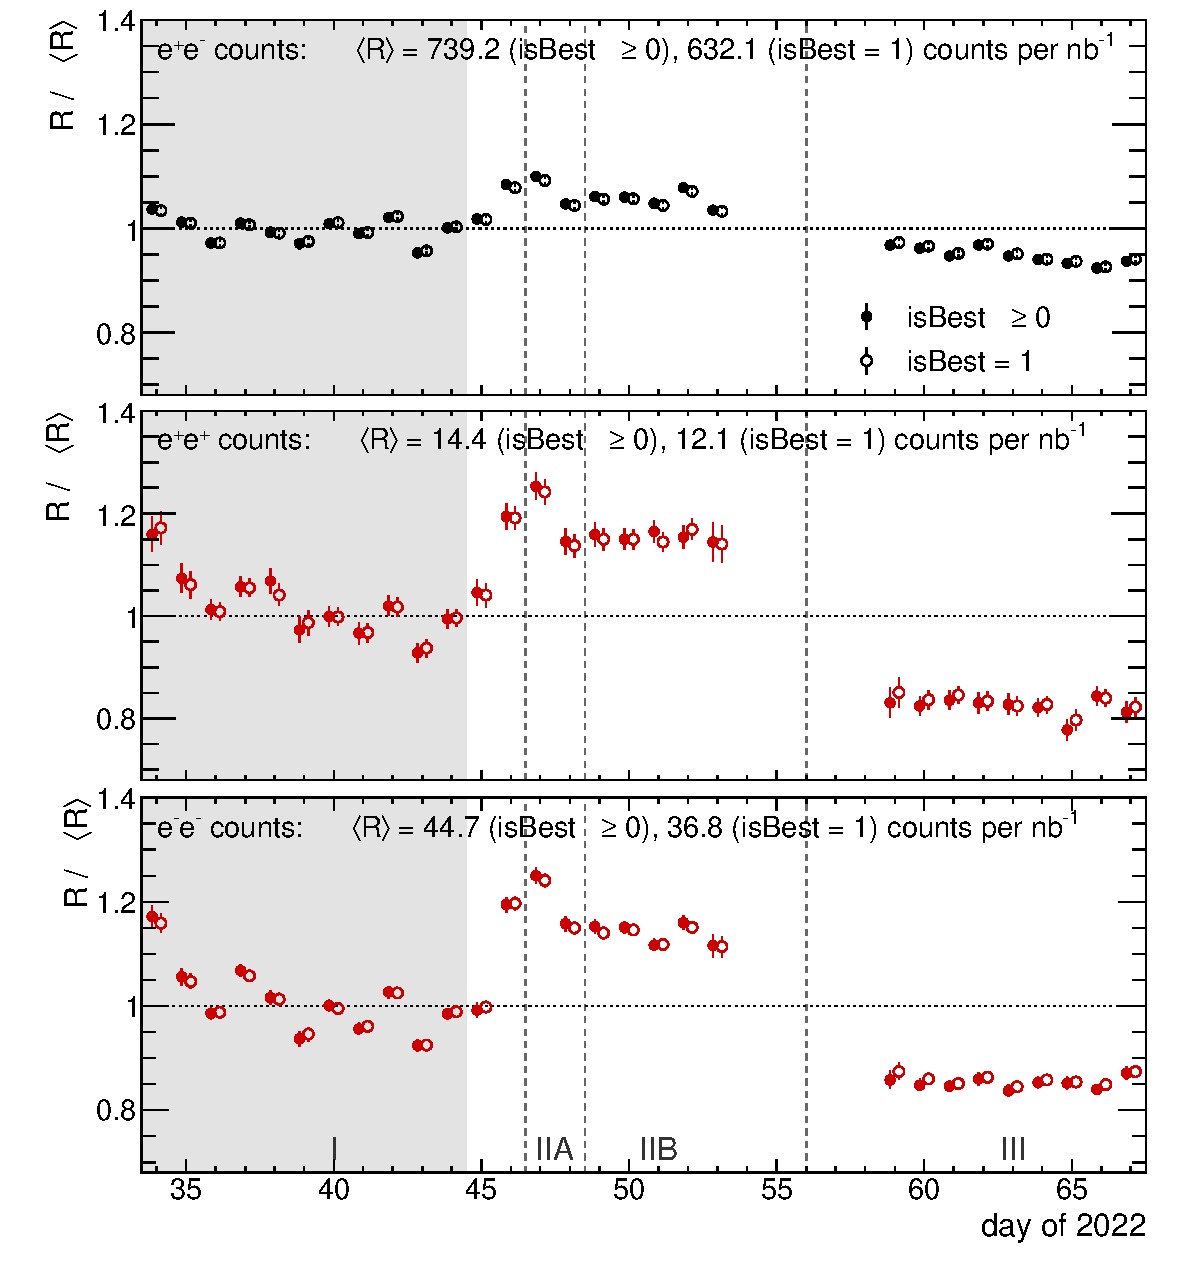
\includegraphics[width=0.62\textwidth]{figs_exp/smp_rates_perday_cnt.pdf}
\caption{\textbf{What it shows: count rates per luminosity change in steps between periods.}
The steps are between the beam periods.
The $\eta$ yield per period nevertheless stays constant within its errors (Fig.~\ref{fig:res-periods}). Selection: data; \ptthreecap{}, event vertex in the target region ($\vz>-160$\,mm), particles identified by their START-free velocity \betanew (pions within $3\sigma$, leptons within $5\sigma$ of their band; leptons with a RICH ring, pions without), energy-loss-corrected momenta of all four tracks (\code{cor_ok} $=1$), all stored \ppee combinations of each event (isBest $\ge0$) (``pre''), all \Mfour, \Mee and \Mpipi, per day; open markers: only the best-ranked combination of each event (isBest $=1$); unlike-sign and like-sign counts with the same cuts, no CB subtracted. The same as Fig.~\ref{fig:smp_rates}: rate per day $R=\text{counts}\times\frac{64}{63}/L$ relative to the
luminosity-weighted mean, for \ee (top), $e^+e^+$ (middle) and $e^-e^-$ counts (bottom), ``pre''; full markers isBest $\ge0$, open isBest $=1$;
grey: days 034--044 with the sector-2 trigger deficit (not in $L$); dashed lines: period boundaries. The \ee rates scatter by 4.9\,\% rms
($\chi^2/\mathrm{ndf}=7206/28$ for a constant): hence the $\pm5$\,\% period-normalisation uncertainty. $L$: START-free luminosity of the
analysed runs ($\Lan=6079.2\,\nbinv\pm6.9$\,\%).}
\label{fig:res-norm}
\end{figure}

\begin{figure}[!tb]
\centering
% Section-1 copy: smp_peak_periods (Section 7)
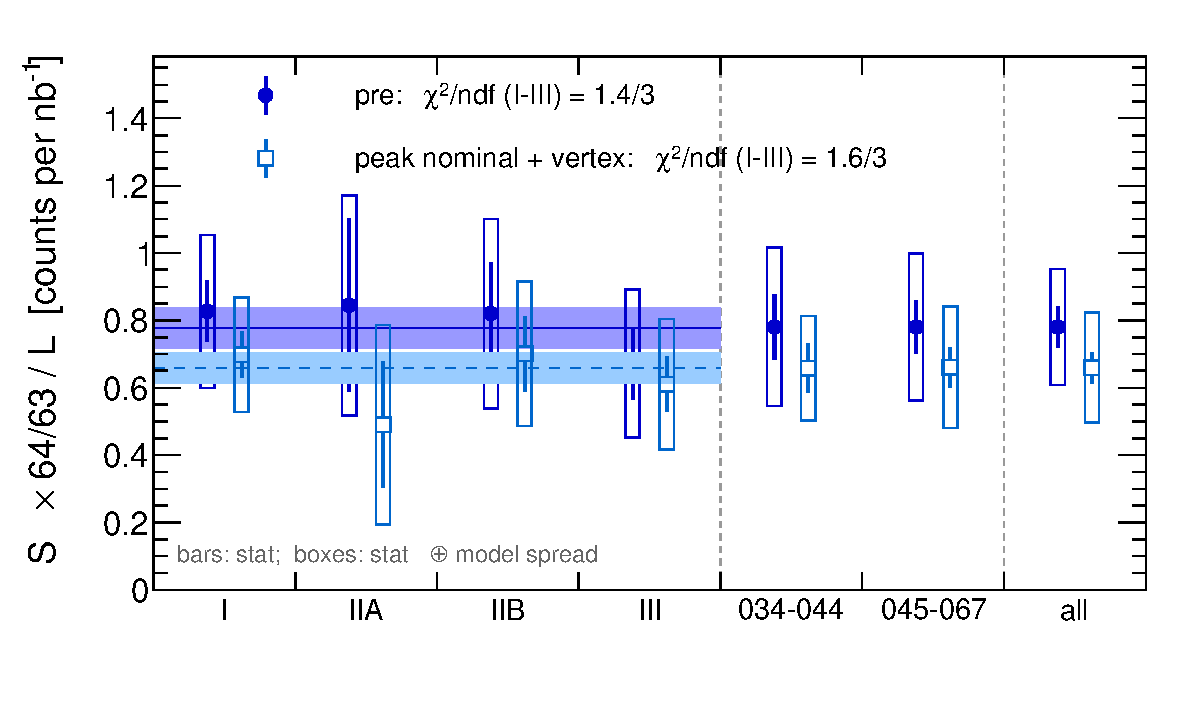
\includegraphics[width=0.66\textwidth]{figs_exp/smp_peak_periods_cnt.pdf}
\caption{\textbf{What it shows: the $\eta$ yield per beam period stays constant within its errors.}
The rates of all counts change in steps between the periods (Fig.~\ref{fig:res-norm}), but the $\eta$-peak yield does not. Selection: data; full circles: \ptthreecap{}, event vertex in the target region ($\vz>-160$\,mm), particles identified by their START-free velocity \betanew (pions within $3\sigma$, leptons within $5\sigma$ of their band; leptons with a RICH ring, pions without), energy-loss-corrected momenta of all four tracks (\code{cor_ok} $=1$), all stored \ppee combinations of each event (isBest $\ge0$) (``pre''); open squares: ``pre'' + the angle between the \pipi and \ee momenta in the laboratory below $55^\circ$ ($\alab<55^\circ$), $\Mpipi>0.30$\,\GeVcc and both pions used in the event-vertex fit (peak nominal + vertex); $S$ from a fit of $N-\mathrm{CB}$ in 0.5225--0.6100\,\GeVcc with a fixed Gaussian (0.5439\,\GeVcc, width 5.4\,\MeVcc) plus a second-order polynomial (\Pmain), CB $=2\sqrt{N_{++}N_{--}}$ from the like-sign counts with the same cuts, $k=1$; periods I (days 034--046), IIA (047--048), IIB (049--053), III (059--067). The same as
Fig.~\ref{fig:smp_periods}: $\eta$-peak yield $S\times\frac{64}{63}/L$ in visible counts per \nbinv per period, for days 034--044 against
045--067, and for all days; ``pre'' (full circles, $\chi^2/\mathrm{ndf}=1.4/3$ over I--III) and peak nominal + vertex (open squares, 1.6/3);
bars: stat; boxes: stat $\oplus$ model spread; bands: weighted mean over I--III (stat). $L$: START-free luminosity of the analysed runs
($\Lan=6079.2\,\nbinv\pm6.9$\,\%, not in the errors); visible yields, not corrected for acceptance or efficiency.}
\label{fig:res-periods}
\end{figure}

\paragraph{10. The target walls give many counts but almost none of the $\eta$.} The luminosity is for the liquid hydrogen (LH$_2$) only, so
reactions in the target walls (the Mylar windows of the cell) and in the material around it must be measured separately. This production of
Part~II holds no empty-target runs; Part~III (package WP2, checked by two independent verifiers with own code) found 127 empty-target runs
of the days 034, 047 and 065, processed them with the same programs and the same selection, and scaled them to the full-target runs of the
same day with the counts in front of the cell, which the beam halo makes in both kinds of runs. Result, from the data alone: the walls give
$13.1\pm0.9$\,\% of the $N-\mathrm{CB}$ counts in 0.40--0.70\,\GeVcc for ``pre'' + both pions in the vertex fit (12.5\,\% after a correction
for the halo level of the empty-target days, 14.7\,\% in the bump and peak windows; $19.0\pm1.1$\,\% for ``pre'' itself, raw), but they
carry almost none of the $\eta$:
in vertex slices of the full 29-day data the $\eta$-peak content per count falls to about zero where the walls give most of the counts
(Fig.~\ref{fig:res-walls}d); the $\eta$ per count in the walls is $r=0.07\pm0.30$ times that in hydrogen, i.e.\ a wall share of the $\eta$
signal $f_\eta=3^{+4}_{-3}$\,\% (Part~III decision D21, approved by the analyst on 15 November 2026). A check with the simulated vertex shape of the hydrogen agrees (cell-centre share of
the $\eta$ $0.566\pm0.045$ and $0.571\pm0.024$ against 0.577; a 16.8\,\% wall share would give 0.497, excluded at 3.4$\sigma$). The narrow
like-sign peak at $\vz=-158.5$\,mm is also in the empty-target runs: it is target material. \emph{Meaning:} the visible $\eta$ yields $S$,
$T$, $E$ and $Y$ of this report contain about 3\,\% $\eta$ from the walls (they would be lower by $3^{+4}_{-3}$\,\% if subtracted; Part~III
applies $1-f_\eta=0.97$, D21, approved by the analyst); the window counts ($N$, $N-\mathrm{CB}$, $W$) contain 16--24\,\% wall counts (``pre'', raw). The wall share of the
counts must never be applied to the $\eta$ yields: the side bands and the background polynomial of the fits already remove the non-peaking
wall counts. \emph{Reliability:} measured (Part~III with two verifiers); the halo normaliser carries $-12/+6$\,\% of the share of the counts, and the
expectation from the nucleon count of the windows (5--12\,\%) is only partly covered by $f_\eta$ (12\,\% lies at 2.3$\sigma$). Figure:
Fig.~\ref{fig:res-walls}; details: \S\ref{sec:walls}.

\begin{figure}[!tb]
\centering
% Section-1 copy of Fig. walls_feta (Section 2.6): the figure of the independent verification vw2a of Part III, WP2
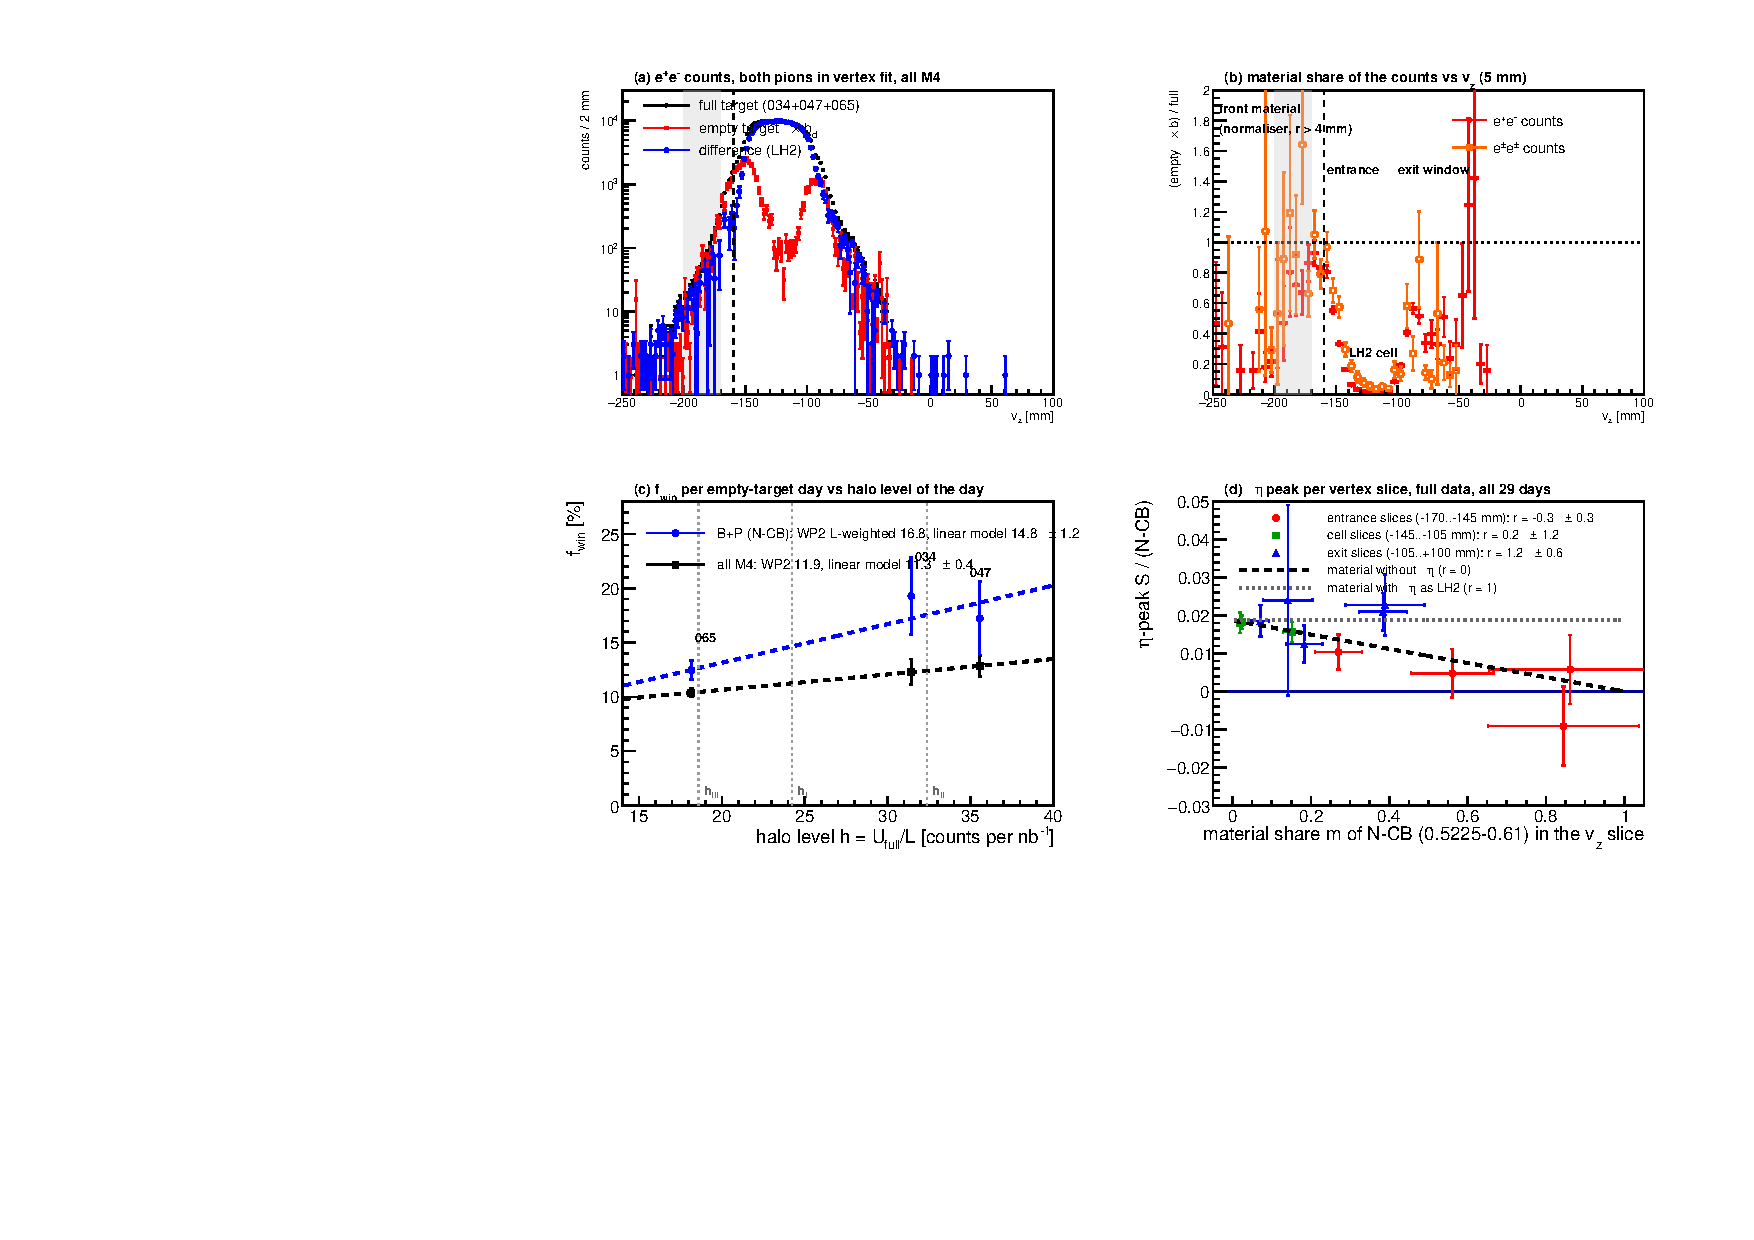
\includegraphics[width=0.72\textwidth]{figs_all/vw2a_fig_cnt.pdf}
\caption{\textbf{What it shows: the target walls give a visible part of the counts, but the $\eta$ signal does not come from them.} Selection: data only. All panels: isBest $\ge0$, a reconstructed event vertex ($\vz>-500$\,mm), \ptthreecap{}, the \betanew particle identification, energy-loss-corrected momenta of all four tracks, both pions used in the event-vertex fit, all \Mfour. (a), (b): days 034 + 047 + 065, no target-region cut (the cut $\vz>-160$\,mm is drawn); (a) \ee counts; (b) \ee and like-sign counts; the empty-target runs scaled with the flux ratio of the same day, from the \ee and like-sign counts with $-200\le\vz<-170$\,mm in front of the cell (no pion-vertex requirement there). (c) with the target-region cut $\vz>-160$\,mm (``pre'' + vertex); $N-\mathrm{CB}$ in all \Mfour and in the bump and peak windows together (0.4550--0.5225 and 0.53364--0.55416\,\GeVcc). (d) full-target runs of all 29 days, no target-region cut, 12 slices of \vz with the edges $-170$, $-160$, $-155$, $-150$, $-145$, $-135$, $-115$, $-105$, $-100$, $-95$, $-85$, $-60$ and $+100$\,mm; in each slice the $\eta$-peak content $S$ (fixed Gaussian plus second-order polynomial, 0.5225--0.61\,\GeVcc) divided by $N-\mathrm{CB}$ in the same range, CB $=2\sqrt{N_{++}N_{--}}$ of the slice, $k=1$.
Data only (full-target runs of all 29 days and the empty-target runs of days 034, 047, 065). The same as Fig.~\ref{fig:walls_feta}
(\S\ref{sec:walls}). (a) Vertex $z$ of the \ee counts (``pre'' + both pions in the vertex fit, all \Mfour), days 034 + 047 + 065: full target
(black), empty target scaled by the flux ratio $b$ of the same day (red), their difference (blue). (b) Material share of the counts per 5\,mm
slice of \vz: the walls dominate at the entrance ($\approx-150$\,mm) and the exit window ($\approx-90$\,mm), inside the cell they give about
1\,\%. (c) Wall share \fwin per empty-target day against the beam-halo level of that day: it follows the halo, and the empty-target days had
a high halo; reweighted to the luminosity-weighted halo, $\fwin(\mathrm{B+P})=14.7\pm1.1$\,\% instead of 16.8\,\%. (d) The decisive test:
$\eta$-peak content per $N-\mathrm{CB}$ count in each \vz slice against the material share of the slice. Walls without $\eta$: dashed line;
walls with $\eta$ like hydrogen: dotted line. The entrance slices (red), where the walls give 30--90\,\% of the counts, fall to about zero
($r=-0.27\pm0.34$ for these slices alone); the exit-window slices are consistent with the hydrogen rate ($r=1.21\pm0.64$); the fit of all
slices gives $r=0.07\pm0.30$, $f_\eta=3^{+4}_{-3}$\,\%. Counts, not normalised to luminosity (panel (c): halo level in counts per \nbinv).}
\label{fig:res-walls}
\end{figure}

\paragraph{11. Inside the peak, close pairs dominate.} Split by the \ee mass (side-band subtraction per class), a share
$0.23\pm0.04\,(\mathrm{stat})\pm0.05\,(\mathrm{method})$ of the peak lies above $\Mee=20$\,\MeVcc, and $0.772\pm0.037$ has OA$>2^\circ$.
Between 5 and 20\,\MeVcc the data hold about $1900\pm400$ counts (about 40\,\% of the peak) more than a direct decay alone would give.
\emph{Meaning:} this would fit $\eta\to\pipi\gamma$ with the photon converted in the material, but the data alone do not prove it
(the estimate assumes the same acceptance for close pairs and for pairs above 20\,\MeVcc). \emph{Reliability:} provisional; the
split into direct decay and conversion is \textbf{not determined} without the simulation (Part~III, with the simulated shapes, finds
relatively fewer conversion pairs in the data than in SMASH and considers a loss of close pairs in the data; D32, ruled on 15 November
2026 to be tested in a separate analysis, \S\ref{sec:needsim}). Figure: Fig.~\ref{fig:res-mee}; details: \S\ref{sec:mee}.

\paragraph{12. Nothing unusual in the X17 band.} A hypothetical 17\,\MeVcc boson from $\eta\to\pipi X17$, $X17\to\ee$ would appear
in the $\eta$-peak counts with $15.5\le\Mee<24.5$\,\MeVcc. There the side-band subtraction leaves $D=481\pm99$ $\eta$ counts, against
$522\pm111$ expected from the neighbouring \Mee bands: the difference, $-40\pm149$, shows nothing. \emph{Reliability:} cross-check (a
look, not a test); a limit on the X17 branching ratio needs the simulated X17 efficiency and is \textbf{not determined} here (Part~III
gives it: $\mathrm{BR}(\eta\to\pipi X17)\,\mathrm{BR}(X17\to\ee)<3.16\times10^{-5}$ at 17\,\MeVcc, 90\,\% CL$_s$, with the PDG 2026
BR$(\eta\to\ppee)$, D25). Figure: Fig.~\ref{fig:res-x17}; details: \S\ref{sec:x17}.

\begin{figure}[!tbp]
\captionsetup{margin=0pt}
% Section-1 copies: panel (a) of res_mee_content and panel (b) of res_x17_window (Section 7)
\begin{minipage}[t]{0.485\textwidth}
\centering
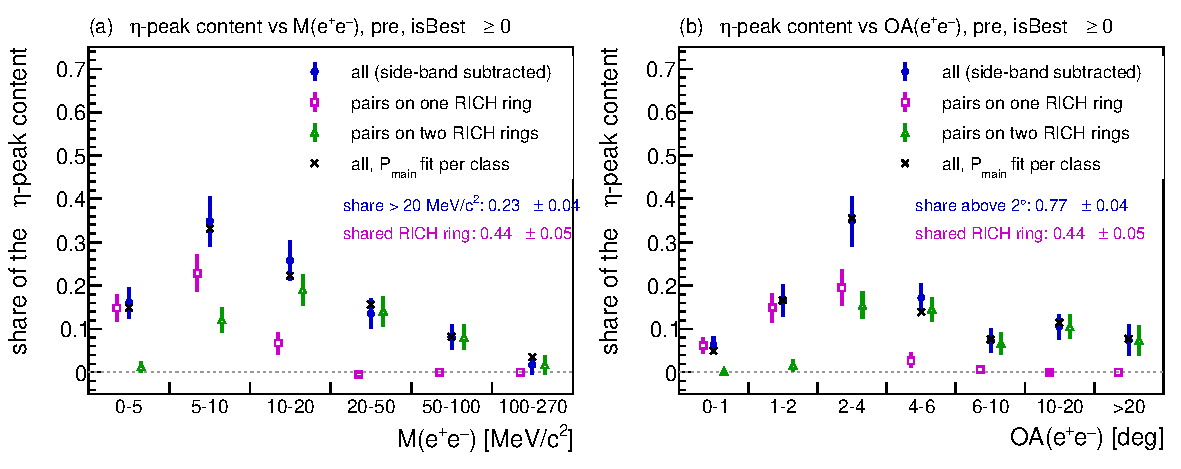
\includegraphics[width=\linewidth,trim=0 0 283 0,clip]{figs_exp/res_mee_content.pdf}
\caption{\textbf{What it shows: close pairs dominate the $\eta$ peak; only 0.23 of it lies above $\Mee=20$\,\MeVcc.} Selection: data; \ptthreecap{}, event vertex in the target region ($\vz>-160$\,mm), particles identified by their START-free velocity \betanew (pions within $3\sigma$, leptons within $5\sigma$ of their band; leptons with a RICH ring, pions without), energy-loss-corrected momenta of all four tracks (\code{cor_ok} $=1$), all stored \ppee combinations of each event (isBest $\ge0$) (``pre''); the \Mee classes 0--5, 5--10, 10--20, 20--50, 50--100 and 100--270\,\MeVcc; $\eta$-peak content of each class from the counts in the data peak window $0.53364\le\Mfour<0.55416$\,\GeVcc minus the background taken from the side bands 0.5225--0.53364 and 0.55416--0.56530\,\GeVcc; CB of each class from the like-sign counts of that class, $k=1$; magenta / green: in addition the two leptons on one shared RICH ring / on two rings.
Panel (a) of Fig.~\ref{fig:res_mee} (\S\ref{sec:mee}): share of the $\eta$-peak content per \Mee class, ``pre'', isBest $\ge0$; blue:
side-band subtraction in \Mfour (stat $\oplus$ model); magenta / green: pairs on one / two RICH rings; crosses: \Pmain fit of each class
alone. Quoted share above 20\,\MeVcc: $0.23\pm0.04\,(\mathrm{stat})\pm0.05\,(\mathrm{method})$; the classes 5--20\,\MeVcc hold about
$1900\pm400$ counts more than a direct decay alone would give. CB of each class from its like-sign counts, $k=1$. Not normalised to luminosity.}
\label{fig:res-mee}
\end{minipage}\hfill
\begin{minipage}[t]{0.485\textwidth}
\centering
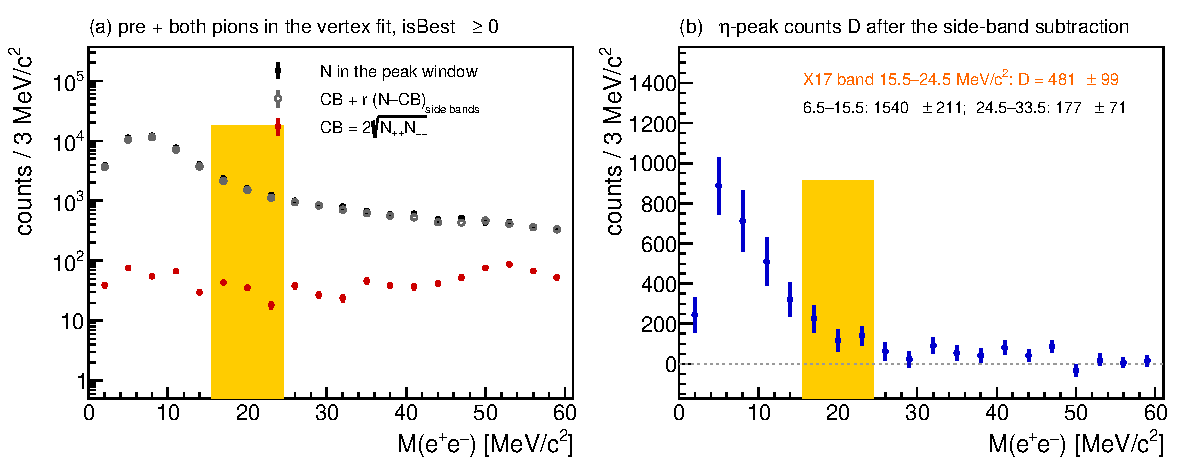
\includegraphics[width=\linewidth,trim=281 0 0 0,clip]{figs_exp/res_x17_window_cnt.pdf}
\caption{\textbf{What it shows: the X17 band holds as many $\eta$ counts as its \Mee neighbours predict.}
No sign of an X17 in the band (orange). Selection: data; \ptthreecap{}, event vertex in the target region ($\vz>-160$\,mm), particles identified by their START-free velocity \betanew (pions within $3\sigma$, leptons within $5\sigma$ of their band; leptons with a RICH ring, pions without), energy-loss-corrected momenta of all four tracks (\code{cor_ok} $=1$), all stored \ppee combinations of each event (isBest $\ge0$), and both pions used in the event-vertex fit (``pre'' + vertex); \Mee from 0.5 to 60.5\,\MeVcc in 3\,\MeVcc bins; $\eta$-peak counts from the counts in the data peak window $0.53364\le\Mfour<0.55416$\,\GeVcc minus the background taken from the side bands 0.5225--0.53364 and 0.55416--0.56530\,\GeVcc; CB of each \Mee bin from the like-sign counts of that bin, $k=1$; X17 band $15.5\le\Mee<24.5$\,\MeVcc, interpolated from the bands 6.5--15.5 and 24.5--33.5\,\MeVcc. Panel (b) of Fig.~\ref{fig:res_x17} (\S\ref{sec:x17}): $\eta$-peak counts $D$ after the side-band subtraction against \Mee (3\,\MeVcc bins),
``pre'' + both pions in the vertex fit, isBest $\ge0$, data peak window 0.53364--0.55416\,\GeVcc. In the band 15.5--24.5\,\MeVcc
$D=481\pm99$, against $522\pm111$ interpolated from the neighbouring bands. No limit is derived (it needs the simulated X17 efficiency).
Not normalised to luminosity.}
\label{fig:res-x17}
\end{minipage}
\end{figure}

\paragraph{13. Production and reconstruction checks.} The committed code reproduces the production bit by bit, and there are no
duplicated entries; a PAT build from the production tag reproduces one full-target DST entry by entry (checked later, for the empty-target runs). The new START-free production ($\betanew$) has $1.38\pm0.17$ times the $\eta$ content of the old one based on the
LGAD start time (the simulation changes only by 1.04). One START-based condition remains in the DST track sorter: 10.6\,\% of the
leptons entered only through its hadron pass, and an event loss of 1.3--1.6\,\% or 2.2--2.8\,\% cannot be excluded and is not
corrected. \emph{Reliability:} identity and cut-flow counts final; the old/new ratio is a cross-check (its error is an upper bound); the
sorter loss is \textbf{not determined} from the output (decision (viii)). Figures: Figs.~\ref{fig:res-oldnew} and~\ref{fig:res-sorter};
details: Appendix~\ref{sec:tech}.

\begin{figure}[!tbp]
\captionsetup{margin=0pt}
% Section-1 copies: left panel of res_oldnew_peak and top-left panel of pid_dstbeta (Appendix C)
\begin{minipage}[t]{0.42\textwidth}
\centering
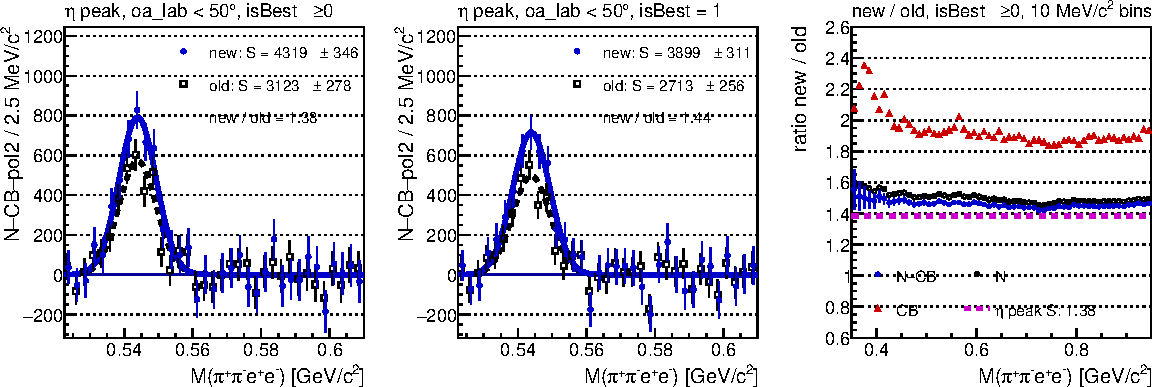
\includegraphics[width=0.95\linewidth,trim=0 0 368 0,clip]{figs_exp/res_oldnew_peak.pdf}
\caption{\textbf{What it shows: the new, START-free production holds 1.38 times the $\eta$ content of the old one.} Selection: data of the same 29 days in both productions, with the cuts of the first study: \ptthreecap{}, a reconstructed event vertex ($\vz>-500$\,mm) but no target-region cut, energy-loss-corrected momenta of all four tracks, all stored combinations (isBest $\ge0$), and the angle between the \pipi and \ee momenta in the laboratory below $50^\circ$ ($\alab<50^\circ$); the particle identification of each production (old: with the LGAD start time; new: \betanew); duplicated entries of the old production removed; CB $=2\sqrt{N_{++}N_{--}}$ from the like-sign counts with the same cuts, $k=1$.
Left panel of Fig.~\ref{fig:oldnew_peak} (Appendix~\ref{sec:oldnew}): $N-\mathrm{CB}-\mathrm{pol2}$, isBest $\ge0$, of the old (LGAD start
time, open squares) and the new ($\betanew$, blue) production, the same 29 days, $\alab<50^\circ$, no $\vz>-160$\,mm cut; CB with $k=1$;
duplicated entries of the old production removed. Ratio $1.38\pm0.17$ (the error is an upper bound); the simulation changes only by 1.04.
Counts, not normalised to luminosity.}
\label{fig:res-oldnew}
\end{minipage}\hfill
\begin{minipage}[t]{0.55\textwidth}
\centering
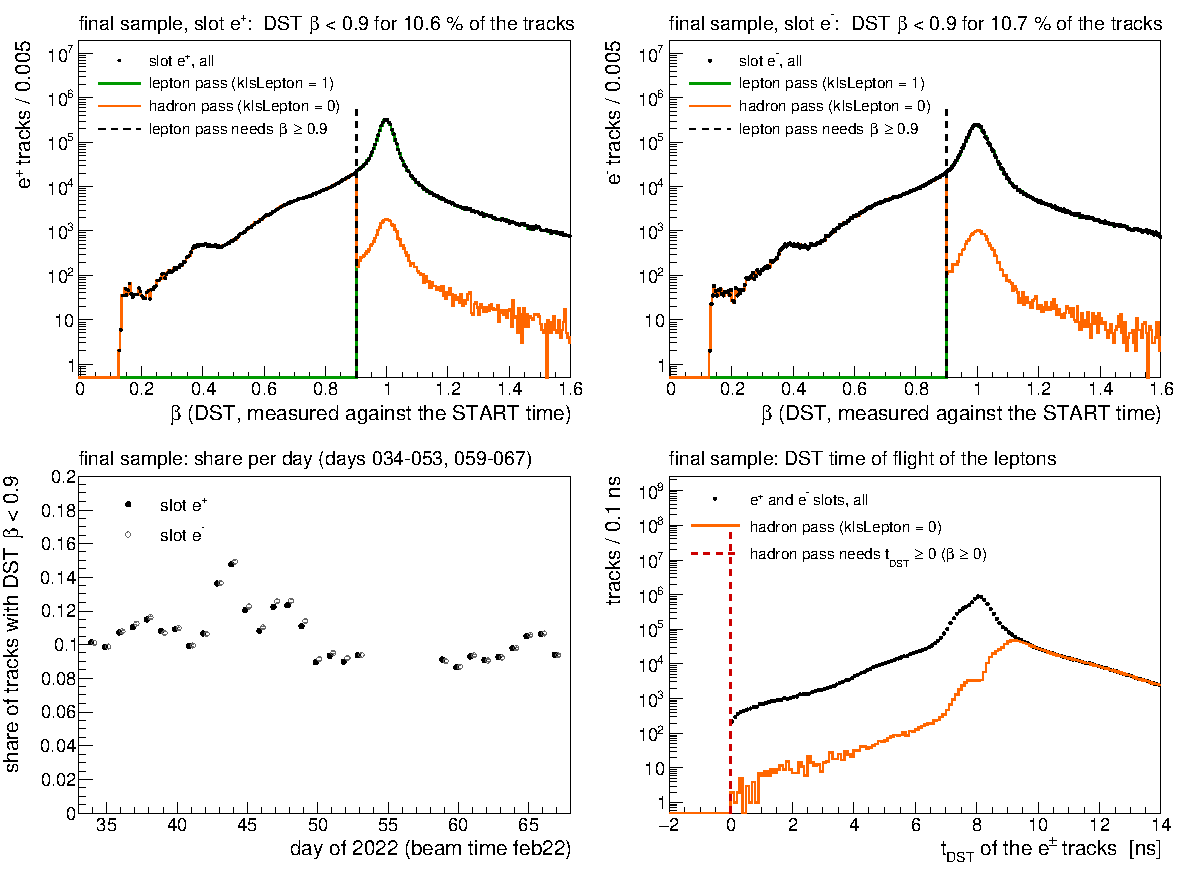
\includegraphics[width=\linewidth,trim=0 206 284 0,clip]{figs_exp/pid_dstbeta.pdf}
\caption{\textbf{What it shows: one START-based condition remains in the track sorter.}
10.6\,\% of the leptons entered only through the hadron pass of the track sorter (orange). Selection: data, all 29 days; the \ppee counts written by FAT: \ptthreecap{}, a reconstructed event vertex ($\vz>-500$\,mm), the \betanew particle identification of PAT, all stored combinations (isBest $\ge0$); no target-region cut and no momentum-correction requirement; the track in the $e^+$ slot of each count. Top-left panel of Fig.~\ref{fig:pid_dstbeta} (Appendix~\ref{sec:sorter}): DST $\beta$ (measured against the START
time) of the $e^+$ slot of the analysed counts (isBest $\ge0$, $\vz>-500$\,mm, PT3, 29 days), tracks accepted by the lepton pass
(\code{kIsLepton} $=1$) and by the hadron pass (\code{kIsLepton} $=0$); dashed: lepton-pass limit 0.9. The $e^-$ slot gives 10.7\,\%, the
simulation 0.01--0.03\,\%. Track counts, not normalised to luminosity.}
\label{fig:res-sorter}
\end{minipage}
\end{figure}

\subsection{What is not determined and why}
\label{sec:notdet}
\begin{itemize}
\setlength{\itemsep}{0pt}
\item \textbf{Efficiencies and cross sections.} The share of the $\eta$ that the detector and the cuts keep must come from the
      simulation; Part~II gives only visible yields (\S\ref{sec:needsim}).
\item \textbf{The bump yield.} $E$ and the step in $u$, $h_u$, show the edge but are not yields; $N-\mathrm{CB}$ in the bump window contains the bump and the
      physical background together, so the extraction needs the simulated bump shape (done in Part~III with the simulation, through
      this edge; \S\ref{sec:needsim}).
\item \textbf{The branching ratio.} In the ratio of the peak to the bump the luminosity and much of the acceptance cancel, but both
      signals contain photon conversions whose probability (the material) does not cancel; they must be subtracted with the
      simulation.
\item \textbf{Direct decay against conversion} in the peak needs the simulated acceptance of each mode in \Mee and OA; \textbf{the
      X17 limit} needs the simulated efficiency of the X17 cuts and the \Mee resolution (both done in Part~III with the simulation,
      \S\ref{sec:needsim}).
\item \textbf{The normalisation of the CB}: correlated $e^-e^-$ sources break the assumption behind the like-sign method, event
      mixing cannot see them, and the simulation does not reproduce the CB; only bounds are given (\S\ref{sec:cbsens}).
\item \textbf{Whether the PT3 live fraction applies} to these events: the data cannot decide (\S\ref{sec:lumi}). \textbf{The
      track-sorter loss}: tracks that fail both passes of the sorter are not written, so it cannot be measured (\S\ref{sec:sorter}).
\item \textbf{The cause of the rate steps} between the beam periods (\S\ref{sec:rates}): they follow the beam-halo level
      (\S\ref{sec:walls}), an indication that still needs a per-day test.
\end{itemize}
\emph{No longer on this list:} the empty-target background. The empty-target runs were found and processed in Part~III with the
programs and the selection of this report; the target walls give 13--15\,\% of the $N-\mathrm{CB}$ counts but only $3^{+4}_{-3}$\,\% of the
$\eta$ signal (measured from the data, \S\ref{sec:walls}).

\subsection{Open questions}
\label{sec:openq}
\begin{itemize}
\setlength{\itemsep}{0pt}
\item The bump $E$ differs between the two fixed halves of the data by $-2.35\sigma$ with the fit errors (about $-2.4\sigma$ with the
      bootstrap errors; the earlier $-2.0\sigma$ used the factor 1.2, which is not confirmed); the 40 random halvings show no general asymmetry
      (mean pull $-0.22\pm0.19$), and Part~III finds $z=1.9$--2.0 ($p\approx0.05$) for the same split on its base, so this one split is
      marginal (\S\ref{sec:stab}).
\item $N-\mathrm{CB}$ turns over near 0.74\,\GeVcc, most likely the edge of $\omega\to\pipi\piz$, $\piz\to\ee\gamma$; not tested
      further (\S\ref{sec:cbnull}).
\item Why neither the counts without an event vertex nor the target-wall counts hold measurable $\eta$ (walls: $r=0.07\pm0.30$ times the
      $\eta$ per count of hydrogen), although p+A collisions at 4.5\,GeV make $\eta$ mesons: from the nucleon count of the Mylar windows
      5--12\,\% of the $\eta$ would be expected; 12\,\% lies at 2.3$\sigma$ (\S\ref{sec:vtxeff}, \S\ref{sec:walls}).
\item Whether the rate steps between the periods are fully explained by the beam halo on the walls and the holder: a per-day test of the
      halo model (\S\ref{sec:walls}); if it holds, the $\pm5$\,\% period normalisation could be reduced.
\item Not checked: which vertex condition the elastic luminosity analysis used (\S\ref{sec:lumi}); without one, upstream elastic events
      add about 1\,\% to $L$; with the DST vertex, the data/simulation difference of the elastic vertex efficiency could reach several
      per cent (not estimated).
\item The two implementations of the sculpting test differ by up to 70 counts (\S\ref{sec:sculpt}); the peak position is not varied in
      the model uncertainty (free fits move by $\pm0.6$\,\MeVcc, \S\ref{sec:scale}).
\item The CB of narrow classes (X17 band, classes above 50\,\MeVcc in \Mee, the counts without a vertex) depends on how the geometric mean
      is built from few like-sign counts (\S\ref{sec:cbmethod}); the side-band numbers $D$ should be insensitive (not evaluated).
\item Why the sector-2 share of the lepton-channel counts is low on day 045 (efficiency $0.903\pm0.007$ in three periods of the day) while
      the elastic events of the same day show no sector-2 deficit in PT2 or PT3 (\S\ref{sec:rates}); the cause was not studied.
\item The height of the step in $u$ without the simulation depends by up to about 7\,\% on how the low-mass tail of the $\eta$ peak is
      modelled (\S\ref{sec:edgeu}); the data cannot measure the size of that tail ($0.3\pm1.0$ times the simulated one; Part~III counts $t=1\pm0.5$ as a systematic term, D40, approved),
      and the data peak counts sit 1.0\,\MeVcc further from their edges than the simulated ones (not understood).
\end{itemize}
\emph{Answered since the first draft:} the narrow like-sign vertex peak at $\vz=-158.5$\,mm, just at the cut $-160$\,mm, is target
material: the same peak is present in the empty-target runs (\S\ref{sec:cutflow}, \S\ref{sec:walls}).

\subsection{Decisions awaiting the analyst's ruling}
\label{sec:decisions}
The most consequential ones, numbered as in the full list (i)--(ix) of Appendix~\ref{app:status}:
\begin{itemize}
\setlength{\itemsep}{0pt}
\item[(i)] the frozen selection PEAK as the final $\eta$-peak selection (\S\ref{sec:recommend});
\item[(ii)] BUMP $=$ ``pre'' (no further cut) for the bump;
\item[(iii)] the frozen X17 cuts, with the X17 \Mfour window moved to the data mass scale, 0.5312--0.5566\,\GeVcc;
\item[(v)] the CB convention $k=1$ kept, with $k_{\mathrm{mix}}$ as a systematic variant;
\item[(viii)] which START-sorter loss (1.3--1.6\,\% or 2.2--2.8\,\%) to carry as a systematic error;
\item[(ix)] the choices of the vertex study: a smooth like-sign CB for the counts without a vertex, $S$, $T$ and $E$ combined as
      independent measures, and the correction quoted as one-sided instead of applied (\textbf{approved} by the analyst on 15 November 2026,
      as Part~III's D33).
\end{itemize}
(ix) is ruled (D33, approved); (i)--(viii) have not been ruled on yet. \textbf{Decisions of Part~III that concern this report}, ruled by
the analyst on 15 November 2026:
D21 approved (the $\eta$ yields of Part~III are multiplied by $1-f_\eta$, $f_\eta=3^{+4}_{-3}$\,\%, never by $1-\fwin$; \S\ref{sec:walls});
D26 approved (the sector-2 deficit span 034--045 of Part~III's correction $C_{\mathrm{sec}}$; the elastic events show that $L$ needs no
sector-2 correction on day 045, \S\ref{sec:rates}); D28 ($\sigma(pp\to\eta X)$ of Part~III keeps its PRELIMINARY label, because the make-up of
the $\eta$ peak is open); D32 (the interpretation ``the data lose close \ee pairs'' is to be tested in a separate analysis,
\S\ref{sec:needsim}); D25 (PDG 2026 everywhere, also for the X17 limit). Ruled in the evening of the same day: D33 approved (the choices
of the vertex study, (ix) above); D37 approved (the step in $u$ is Part~III's bump measurement, the per-slice edge its cross-check); D38
approved (the simulated C2 Dalitz decays of Part~III get per-count QED weights for the decay angle, until a future simulation corrects the
angle in GEANT itself, which is not expected); D39 approved (the origin of the $e^-e^-$ step in $u$ recorded, the CB kept; independently
verified); D40 approved, option (a) (the low-mass tail of the $\eta$ peak: the simulated tail kept as nominal and half of it taken as a
systematic term, $\pm3.4$\,\% on the bump scale of Part~III and $\pm8.8$\,\% on $\sigma(pp\to\eta X)$ from the peak; $h_u$ of this report does
not change). With these, all of Part~III's decisions D21--D40 are ruled.

\subsection{Symbols used in this section}
\label{sec:symbols}
{\footnotesize
\setlength{\tabcolsep}{4pt}
\renewcommand{\arraystretch}{1.06}
\begin{longtable}{@{}>{\raggedright\arraybackslash}p{3.3cm} >{\raggedright\arraybackslash}p{\dimexpr\textwidth-3.3cm-2\tabcolsep\relax}@{}}
\toprule
count & one stored combination \pip\pim$\ell\ell$ of four tracks (one ntuple entry); with isBest $\ge0$ an event can give more than one count \\
all combinations, isBest & isBest $\ge0$: all stored combinations of an event (main variant); isBest $=1$: only the best-ranked one \\
``pre'' & base selection: all combinations, corrected momenta for all four tracks, event vertex $\vz>-160$\,mm (and the FAT conditions $\vz>-500$\,mm and trigger PT3) \\
PEAK, DIRECT, BUMP, X17 & selections frozen in the simulation study (Part~I): PEAK $=$ ``pre'' + $\dzpi<40$\,mm + $\MMfour<2.85$\,\GeVcc; DIRECT $=$ ``pre'' + $\dzpi<40$\,mm; BUMP $=$ ``pre''; X17 band $=$ ``pre'' + both pions in the event-vertex fit + $15.5\le\Mee<24.5$\,\MeVcc \\
peak / bump nominal + vertex & selections optimised on these data: ``pre'' + $\alab<55^\circ$ + $\Mpipi>0.30$\,\GeVcc (peak) or $\alab<40^\circ$ + $0.30<\Mpipi<0.41$\,\GeVcc (bump), each + both pions in the event-vertex fit \\
\Mfour, \Mee, \Mpipi, OA & invariant masses of \ppee, of the \ee pair and of the \pipi pair; opening angle of $e^+$ and $e^-$ \\
\dzpi, \MMfour, \alab & largest distance in $z$ of the two pion tracks from \vz; missing mass of \ppee; angle between the \pipi and the \ee momenta \\
$N$, $N_{++}$, $N_{--}$ & counts of the \ppee hypothesis and of the like-sign hypotheses \pipi$e^+e^+$ and \pipi$e^-e^-$ \\
CB, $k$, $k_{\mathrm{mix}}$ & combinatorial background $k\cdot2\sqrt{N_{++}N_{--}}$ per 10\,\MeVcc of \Mfour; convention $k=1$; $k$ measured by event mixing \\
$S$, stat, model, $F$ & $\eta$-peak content of the \Pmain fit of $N-\mathrm{CB}$; its fit error; the rms over the edge-safe fit variations that pass $p>0.05$ (90 of 144 for PEAK); $F=S/\mathrm{stat}$, which compares selections and is not a significance \\
$Y$, $Y_T$ & visible yield $S\times\frac{64}{63}/\Lan$ (or the same for $T$) in visible counts per \nbinv; not a cross section \\
$E$, $T$ & bump edge step summed over four \Mpipi slices, counts per 2.5\,\MeVcc, not a yield; ECAL-tagged $\eta\to\pipi\piz$ content \\
$u$, \Medge, $h_u$ & distance to the kinematic edge of the bump, $u=\Mfour-\Medge$; the edge $\Medge(\Mpipi,\Mee)$ of every count (largest \Mfour of $\eta\to\pipi\piz$, $\piz\to\ee\gamma$ with the photon lost, for the measured \Mpipi and \Mee; Part~III writes it $E(m,q)$, here $E$ is the per-slice measure); height of the step at $u=0$, counts per 2.5\,\MeVcc, not a yield \\
$t$ & size of the low-mass tail of the $\eta$ peak relative to the simulated tail (Part~III): $t=1$ SMASH, $t=0$ no tail \\
$\varepsilon_{\mathrm{vtx}}$ & share of the $\eta$ kept by the mandatory cut $\vz>-500$\,mm \\
\Lan & START-free luminosity of the 17\,557 analysed runs, 6079.2\,\nbinv \\
$D$ & $\eta$-peak counts after a side-band subtraction in \Mfour \\
$S_{\mathrm{fake}}$ & peak content that a cut makes from a smooth spectrum without an $\eta$ (sculpting test) \\
START, LGAD, \betanew & START: the start-time detector, whose time in the feb22 data is not always right; LGAD: the start time used by the old production; \betanew: velocity from the time differences of the tracks of one combination, so a START error cancels (START-free) \\
track sorter, hadron pass & DST track sorter: chooses the track candidates in two passes, a lepton pass (DST $\beta\ge0.9$) and a hadron pass (DST $\beta\ge0$, tof $\le60$\,ns); DST $\beta$ is measured against the START time \\
PT3/PT2 live fraction & $L$ contains the live fraction of the trigger PT2; ratio of the live fractions of PT3 (this analysis) and PT2, 0.932 with the trigger-bit factor; whether it applies cannot be decided with the data \\
sector-2 deficit & hardware trigger deficit in sector 2 ($\varphi=180$--$240^\circ$) on days 034--044 (intermittent; on day 045 only in the lepton channel, not in the elastic events), not in $L$; it loses 1.2\,\% of the counts of the sample \\
ECAL sector~0 & the ECAL sector at azimuth 63--117$^\circ$, switched off in the data and in the simulation (not the tracking sector~2 of the trigger deficit) \\
K$^0_S$ & neutral kaon decaying to \pipi with a displaced crossing point; it fixes the \Mpipi mass scale \\
target walls, empty target & the Mylar windows of the LH$_2$ cell and the material around it; runs with the cell empty measure them \\
$U$, $b$, $h$ & counts with $-200\le\vz<-170$\,mm (beam halo on material in front of the cell); flux ratio $b=U_{\mathrm{full}}/U_{\mathrm{empty}}$ of the same day; halo level $U/L$ (counts per \nbinv) or $h=100\,U/N$ (per 100 counts of ``pre'' + vertex) \\
\fwin, \feta & share of the target walls in the $N-\mathrm{CB}$ counts of a window ($b\times$ empty / full); in the $\eta$ signal ($3^{+4}_{-3}$\,\%) \\
\bottomrule
\end{longtable}
\addtocounter{table}{-1}% uncaptioned longtable: do not use up a table number
}
\vspace{-1.2em}The full notation is in Table~\ref{tab:notation} (Appendix~\ref{app:notation}).
\enlargethispage{2\baselineskip}% layout only (16 Nov 2026): keeps the last contents line on this page

\vspace{1.5em}
\setcounter{tocdepth}{1}% contents: sections only and compact, as in Part III, so that they end on the page where they start
\begingroup\setlength{\parskip}{0pt}\let\origaddvspace\addvspace\renewcommand{\addvspace}[1]{\origaddvspace{0.25em}}
\tableofcontents
\endgroup
\setcounter{tocdepth}{3}% (subsections stay in the PDF bookmarks)

\howpart{How the results were obtained}

%======================================================================
\section{Scope}
\label{sec:scope}
%======================================================================

\inshort{Part~II uses the experimental data alone. It gives visible yields (counts per \nbinv, not corrected for efficiency), the CB, the selection and the checks; what needs the simulation is listed in \S\ref{sec:needsim}. The conventions below hold for every number.}
This part documents the analysis of the experimental data of the final state \ppee in p+p collisions
at $T=4.5$\,GeV (feb22 beam time, 29 days, PT3 trigger). As in Part~I, two $\eta$ structures are
expected in \Mfour:
\begin{itemize}
\item the \textbf{peak} at $m_\eta$, from the decay $\eta\to\ppee$ and from $\eta\to\pipi\gamma$ when
      the photon converts into an \ee pair in the detector material;
\item the \textbf{bump} below $m_\eta$, from $\eta\to\pipi\piz$ followed by $\piz\to\ee\gamma$ when the
      photon is lost (and by a photon conversion, which cannot be told apart).
\end{itemize}
The \ee pairs of the peak are also where a hypothetical X17 boson ($\eta\to\pipi X17$, $X17\to\ee$)
would show up.

Part~II covers everything that the data can tell \emph{without} the simulation. The results are collected in plain words in
\S\ref{sec:results}; the chapters below show how they were obtained: the data sample and
its luminosity (\S\ref{sec:data}), the analysis
chain and the particle identification (\S\ref{sec:ana}), the spectra and the combinatorial background
(\S\ref{sec:spec}), the optimisation of the selection on the data together with the selections frozen in
the simulation study (\S\ref{sec:opt}), and the results that need no simulation (\S\ref{sec:res}).
What needs the simulation (efficiencies, the bump yield, the branching ratio, the X17 limit) is listed in
\S\ref{sec:needsim} and is the subject of the next report. Technical points met on the way are in Appendix~\ref{sec:tech}.

\notebox{\textbf{Conventions used in every number of this report} (stated again in the captions).
\begin{enumerate}
\setlength{\itemsep}{0pt}
\item Beam kinetic energy $T_{\mathrm{beam}}=4530$\,MeV in all kinematics; momenta corrected for the energy loss (COR);
      only entries with \code{cor_ok} $=1$ (no fallback).
\item All stored combinations, isBest $\ge0$, are the main variant; isBest $=1$ is the comparison
      variant (``isBest $=0$'' alone is never used).
\item Event vertex $\vz>-500$\,mm (FAT, mandatory); the analysis cut $\vz>-160$\,mm is adopted.
      PT3 trigger, \code{trigbit} $==8192$.
\item $\mathrm{CB}=2\sqrt{N_{++}N_{--}}$ per 10\,MeV bin of \Mfour from the like-sign hypotheses,
      interpolated to the 2.5\,MeV bins, $k=1$; the sensitivity to a $\pm3$\,\% CB change is quoted.
\item OA$(\ee)>2^\circ$ is not a fixed cut: numbers are given with and without it.
\item ECAL is used for verification only (the tagged $\eta$).
\item Event groups $=$ adjacent entries with equal (\code{file_id}, run, event); the errors of window counts,
      fractions, ratios and side-band numbers treat the counts of one event group as correlated. The fit
      errors of \Pmain, $E$ and $T$ are per-count Poisson errors: the group term would enlarge the errors of
      $S$ by 0.8--1.6\,\%; independent halves of the data find the $S$ errors right, and a bootstrap with 200 replicas
      (Part~III) finds the $E$ errors right (the factor 1.2 of 40 halvings of the earlier draft is not confirmed; \S\ref{sec:fixmodel}).
\item Data-only numbers use the \emph{data} windows (peak 0.53364--0.55416, bump 0.4550--0.5225\,\GeVcc).
      The frozen windows of the simulation study are centred on the simulated peak and are used only
      where this is said.
\end{enumerate}}

All counts are stored combinations (one ntuple entry each), not events, and are not corrected for acceptance or efficiency. Where a
yield is normalised to the luminosity it is a \emph{visible} yield in visible counts per \nbinv (counts, not
events: with isBest $\ge0$ an event can give more than one count; not a cross section):
\begin{equation}
Y_X = X \times \frac{64}{63}\,\Big/\,\Lan, \qquad \Lan = 6079.2\,\nbinv,\qquad X=N,\ S\ \text{or}\ T,
\label{eq:yield}
\end{equation}
with the luminosity uncertainty ($\pm6.9$\,\%, and the one-sided live-fraction effect of
\S\ref{sec:lumi}) kept apart. The numbers come from seven chapters of the data study (prefixes
\code{prep}, \code{smp}, \code{pid}, \code{spec}, \code{cb}, \code{opt}, \code{res}); each chapter was
checked by an independent analyst who re-derived the key numbers with own code from a different input
path (the FAT ntuples instead of the compact file, own fits). The macros and the commands are listed in
Appendix~\ref{app:files}. The measurement procedures (the $\eta$-peak content $S$ of the \Pmain fit, its precision $F$, the
bump edge step $E$, the efficiencies $\varepsilon_S$) are defined in \S\ref{sec:proc} and are used before that section where needed.

%======================================================================
\section{Data sample and luminosity}
\label{sec:data}
%======================================================================

\inshort{29 day files of the feb22 beam time; FAT keeps 4\,783\,467 \ee entries, ``pre'' 4\,423\,338. The luminosity of the analysed runs is $\Lan=6079.2\,\nbinv\pm6.9$\,\%; three one-sided effects, not corrected in the yields, could make them up to about 11\,\% too low, and the count rates change in steps between the periods ($\pm5$\,\% on the integrated yields; the steps follow the beam halo, an indication). The mandatory event-vertex cut removes 32\,\% of the \ee counts, but keeps $0.994\pm0.021$ of the $\eta$ (\S\ref{sec:vtxeff}). The target walls, measured with empty-target runs, give 13--15\,\% of the $N-\mathrm{CB}$ counts but only $3^{+4}_{-3}$\,\% of the $\eta$ (\S\ref{sec:walls}). The elastic events of day 045 show no sector-2 deficit, so $L$ needs no sector-2 correction on that day; the low sector-2 share of our counts on day 045 belongs to the lepton channel (\S\ref{sec:rates}).}

\subsection{PAT production}
\label{sec:prod}
The data are the 29 day files of the feb22 beam time, \code{lep_034} \dots\ \code{lep_053} and
\code{lep_059} \dots\ \code{lep_067} (days 054--058 have no data), 383.6\,GB in total (decimal; 4.83\,GB
for day 059 to 21.28\,GB for day 050), list \fpath{/hdd3/przygoda/HADES/files/exp/gen4/lep_betanew.list}.
They were produced by PAT (repository \code{pat3}, annotated tag \code{prod-feb22-betanew-2026-10-28}:
\code{ana} built from commit \code{0129bf3}, scripts \code{e54e6bd}), Hydra~2.7.6, ROOT~6.36.02,
Debian~12. The particle identification uses $\betanew$ with the data polygons
\code{pp45_pid_cuts_exp_betanew_v1.root} (\S\ref{sec:pid}). Hypotheses rejected by the PID are not written:
there are no entries with isBest $<0$, and every event has exactly one entry with isBest $=1$.

The day files were merged from the PAT outputs of the official DST lists (176\,084 DSTs, the DST set of
the luminosity table; the DSTs of days 048/061 with a wrong magnet current are excluded). 586 DSTs were
not merged; all are classified as empty (PAT extracts no particle: broken \code{HParticleCand}). Each day
file holds three hypothesis trees, \code{PipPimEpEm_ID} (unlike-sign), \code{PipPimEpEp_ID} and
\code{PipPimEmEm_ID} (like-sign), and the pair tree \code{EpEm_ID} used here only to list the runs.
Table~\ref{tab:smp_samples} gives the files with their entries, runs and luminosity.

% smp_samples_cnt.tex: copy of smp_samples.tex with "rows" -> "counts" (analyst, 15 Nov 2026; Part II writer, integ4)
% smp_samples.tex -- written by plots/exp_report/smp_report.C (numbers: tables_exp/smp_samples.txt)
\begin{table}[H]
\centering\footnotesize
\setlength{\tabcolsep}{3.5pt}
\caption{Experimental data sample: the 29 day files of the beam time (feb22, p+p, $T=4.53$~GeV) read by FAT (PAT production tag \texttt{prod-feb22-betanew-2026-10-28}, Hydra 2.7.6, PID on $\beta_\mathrm{new}$ with the polygons \texttt{betanew\_v1}). PAT entries = stored particle combinations of the three hypothesis trees before any FAT cut. Runs: in the luminosity table / present in the data (runs with $e^+e^-$ pair entries). $L$: START-free luminosity (six sectors) of all runs and of the analysed runs, in nb$^{-1}$.}
\label{tab:smp_samples}
\begin{tabular}{llr rrr rr rr}
\toprule
 & & & \multicolumn{3}{c}{PAT entries $\pi^+\pi^-\ell\ell$} & \multicolumn{2}{c}{Runs} & \multicolumn{2}{c}{$L$ [nb$^{-1}$]} \\
\cmidrule(lr){4-6}\cmidrule(lr){7-8}\cmidrule(lr){9-10}
Day & Period & GB & $e^+e^-$ & $e^+e^+$ & $e^-e^-$ & all & present & all & analysed \\
\midrule
034 & I & 7.7 & 136047 & 9400 & 33104 & 312 & 309 & 99.8 & 99.8 \\
035 & I & 8.7 & 164358 & 9852 & 36563 & 377 & 375 & 134.5 & 134.5 \\
036 & I & 17.1 & 324071 & 19519 & 70367 & 768 & 767 & 281.5 & 281.5 \\
037 & I & 18.8 & 361262 & 21877 & 78918 & 784 & 784 & 301.1 & 301.1 \\
038 & I & 11.7 & 222410 & 13536 & 47943 & 491 & 487 & 188.7 & 188.7 \\
039 & I & 8.8 & 164703 & 9586 & 34439 & 432 & 428 & 147.2 & 145.9 \\
040 & I & 16.3 & 308156 & 17986 & 65147 & 743 & 740 & 262.1 & 262.1 \\
041 & I & 14.1 & 266497 & 15359 & 55388 & 635 & 633 & 232.9 & 232.9 \\
042 & I & 16.2 & 307676 & 17531 & 64889 & 708 & 702 & 260.5 & 260.5 \\
043 & I & 14.8 & 276953 & 15792 & 57265 & 733 & 729 & 252.4 & 252.4 \\
044 & I & 17.6 & 334221 & 19147 & 69837 & 832 & 823 & 289.7 & 289.7 \\
045 & I & 10.5 & 199681 & 11255 & 41497 & 522 & 520 & 170.4 & 170.4 \\
046 & I & 13.9 & 256507 & 16363 & 60142 & 596 & 596 & 189.8 & 189.8 \\
047 & IIA & 15.3 & 269408 & 17869 & 67551 & 673 & 668 & 185.0 & 185.0 \\
048 & IIA & 14.4 & 253203 & 16523 & 62612 & 651 & 649 & 187.6 & 187.6 \\
049 & IIB & 17.1 & 304053 & 19712 & 74698 & 767 & 765 & 223.3 & 223.3 \\
050 & IIB & 21.3 & 376354 & 24468 & 93069 & 865 & 864 & 275.9 & 275.8 \\
051 & IIB & 20.7 & 364700 & 23832 & 90030 & 858 & 858 & 270.0 & 270.0 \\
052 & IIB & 18.0 & 321972 & 20993 & 79915 & 706 & 705 & 231.5 & 231.5 \\
053 & IIB & 5.9 & 104099 & 6865 & 26141 & 231 & 231 & 77.5 & 77.5 \\
059 & III & 4.8 & 94982 & 4799 & 18283 & 227 & 226 & 90.0 & 90.0 \\
060 & III & 11.3 & 221953 & 11311 & 42756 & 564 & 564 & 212.8 & 212.8 \\
061 & III & 12.9 & 254803 & 13209 & 48660 & 714 & 709 & 247.9 & 247.9 \\
062 & III & 10.5 & 207687 & 10465 & 39778 & 538 & 538 & 197.4 & 197.4 \\
063 & III & 10.9 & 214685 & 10822 & 41178 & 589 & 589 & 208.6 & 208.6 \\
064 & III & 12.4 & 244547 & 12478 & 47204 & 636 & 636 & 240.6 & 240.6 \\
065 & III & 8.8 & 172515 & 8675 & 33481 & 460 & 459 & 170.0 & 170.0 \\
066 & III & 13.7 & 269734 & 14371 & 52107 & 729 & 729 & 267.0 & 267.0 \\
067 & III & 9.6 & 188918 & 9635 & 36454 & 474 & 474 & 184.7 & 184.7 \\
\midrule
Total & & 383.6 & 7186155 & 423230 & 1569416 & 17615 & 17557 & 6080.5 & 6079.2 \\
\bottomrule
\end{tabular}
\end{table}


\subsection{Processing by FAT}
\label{sec:fat}
FAT (this repository, branch \code{pp45_pippimepem}, commit \code{38d168f}) reads the three trees with the
configurations \code{config.json}, \code{config_epep.json}, \code{config_emem.json}; they differ only in
the tree, the lepton prefixes and the output name. The like-sign trees are read through a prefix mapping,
so the same code and the same cuts act on all three hypotheses. One call of the event loop is one ntuple entry.
FAT rejects an entry only by these three conditions, in this order:
\begin{enumerate}
\item isBest $\ge0$ (in practice no effect: every PAT entry has isBest 0 or 1);
\item event vertex $\vz>-500$\,mm (mandatory; removes the entries without a reconstructed vertex);
\item PT3: \code{trigbit} $==8192$ (trigger bit 8192; no trigger-bias weights).
\end{enumerate}
Everything else (the cuts of \S\ref{sec:sel}, the ECAL flags, \code{cor_ok}) is stored as a value or a
flag in the ntuple \code{scan_nt} (145 columns per entry). There is no START or LGAD requirement; the
column \code{evtStart} is only stored. The production ran on 2026-11-11 from 04:56 to 05:07 in 29 parts,
all of which ended without error, and wrote
\fpath{/hdd3/przygoda/HADES/FAT_out/exp/pippimepem_isBestAll_T4530/output_pippim<hyp>_exp.root} with
\code{<hyp>} $=$ \code{epem}, \code{epep}, \code{emem}:
4\,783\,467, 122\,875 and 371\,524 entries in 4\,058\,586, 102\,559 and 302\,701 events (1.18, 1.20 and
1.23 entries per event).

The macro \fpath{plots/scan_prepare.C} turns the three outputs into the compact file
\fpath{scan_v2/scan_compact.root} (trees \code{us}, \code{pp}, \code{mm}) that all analysis macros read:
it forms the event groups (\S\ref{sec:groups}), the fold, the crossing points of the lepton and pion
tracks, the photon closest to the \piz mass, and the pion-vertex variables of \S\ref{sec:dzpivar}. Its
read-back check compares every entry with \code{scan_nt} (0 mismatches).

\textbf{The trigger PT3.} PT3, the main reaction trigger of the feb22 beam time, requires fullSecMult\,$\ge2$ and
iTOFPadMult\,$\ge3$: fullSecMult counts the sectors in which a hit of the inner TOF wall (iTOF) is in coincidence with a hit
of the TOF wall or of the RPC of the same sector, and iTOFPadMult counts the hit iTOF paddles. In words: at least two sectors
with an inner-TOF hit in coincidence with TOF or RPC, and at least three inner-TOF paddles hit. PT2, the minimum-bias trigger,
requires fullSecMult\,$\ge1$ and is downscaled by 64. In the feb22 data only the bit of the trigger that arrives first is
written: PT3 events carry bit 8192, while PT2 events and events with both PT2 and PT3 carry bit 4096. The events with bit 8192
therefore hold 63/64 of all PT3 events, and every visible yield is multiplied by 64/63 (\S\ref{sec:lumi}). Source:
P.~Tlusty, ``LVL1 trigger in Feb22 p+p 4.5\,GeV'', HADES internal presentation, 13 December 2024, with the definition
slide of I.~Ciepa{\l}.

\subsection{Luminosity}
\label{sec:lumi}
The luminosity comes from the START-free analysis of elastic p+p scattering of HADES (talk
``LGADfree\_luminosity\_talk\_draft\_v2''; ``revision N'' is the version label of its result files, 2026-11-04). For all 17\,615 runs and
six sectors
\begin{align*}
\Lsf = 6080.5 &\pm 5.2\,(\mathrm{stat}) \pm 337.9\,(\text{HADES syst.}, 5.56\,\%)\\
&\pm 62.6\,(\sigma_{\mathrm{int}}\text{ fit}, 1.03\,\%) \pm 243.2\,(\text{Argonne normalisation}, 4.0\,\%)\ \nbinv,
\end{align*}
6.9\,\% in total. The per-sector uncertainty of Table~\ref{tab:smp_lumi} is a part of the 5.56\,\% and must
not be added again.

\textbf{Runs present in the data.} A run counts as analysed when the day file contains \code{EpEm_ID} entries
of it: 17\,557 of the 17\,615 runs. The 58 missing runs have no reconstructed particles in the lepton
production, and 52 of them have $L=0$ anyway. Summed over the present runs,
$\Lan=6079.2\,\nbinv$, 0.022\,\% below \Lsf (6079.17 if the two partly merged runs are scaled by their
merged fraction). Per day \Lan differs from \Lsf only on day 039 (three runs without merged DSTs) and on
day 050. All yields per luminosity in this report use \Lan.

\textbf{Rules for a PT3 analysis} (from the header of the luminosity files, each with its procedure here):
\begin{enumerate}
\item \textbf{Trigger bit.} 1/64 of the PT3 events carry bit 4096 instead of 8192 (\S\ref{sec:fat}). FAT selects
      exactly \code{trigbit} $==8192$, so every visible yield is multiplied by $64/63=1.01587$, Eq.~(\ref{eq:yield}).
      The same selection also drops 335/11/22 entries (us/pp/mm) with \code{trigbit} $=12288$ (both bits) and one entry with 131072
      (0.007\,\%, negligible).
\item \textbf{Live fraction.} $L$ contains the live fraction of PT2. The luminosity files give the PT3/PT2
      live-fraction ratio already multiplied by the trigger-bit factor, $f_{\mathrm{LF}}=\mathrm{LF3}/\mathrm{LF2}\times64/63$
      (``with this factor'' in the file header), 0.932 overall and 0.900--0.948 per day. This does not count
      the 64/63 twice: if the correction is applied, $Y=N\times\frac{64}{63}/(L\,f_{\mathrm{LF}})=N/(L\,\mathrm{LF3}/\mathrm{LF2})$,
      and the two factors cancel. It is not known whether the ratio applies to single-interaction PT3 events,
      and the data cannot decide (\S\ref{sec:rates}). It is kept as a one-sided uncertainty with the value of the
      file, 0.932: $L$ may be up to 6.8\,\% lower, so the yields per luminosity may be up to 7.3\,\% higher
      ($1/0.932$). (Our own $L$-weighted mean of the per-day values is 0.9334, $\Lan f_{\mathrm{LF}}=5674.5\,\nbinv$;
      the difference to 0.932 comes from the weighting and is immaterial.)
\item \textbf{Sector 2, days 034--044.} A hardware trigger deficit that is \emph{not} in $L$ (the factor
      1.058--1.120 of the luminosity analysis corrects only its own PT2 elastic count). It must be handled
      in the trigger efficiency of this analysis; \S\ref{sec:rates} estimates it. The analyst's per-day counts of elastic events per sector
      (added on 15 November) show the PT2 deficit on days 041--044 (0.65--0.76 of the clean-day ratio) and none on day 045 (1.074 in PT2 and in
      PT3, Table~\ref{tab:s2pt2}): $L$ is right on day 045 without a sector-2 correction.
\item \textbf{Empty target.} $L$ is for LH$_2$ only; yields should be empty-target subtracted. The production of this
      report holds no empty-target runs, but 127 such runs exist; Part~III processed them with the same programs and
      selection and measured the share of the target walls (\S\ref{sec:walls}): 13--15\,\% of the $N-\mathrm{CB}$ counts,
      but only $3^{+4}_{-3}$\,\% of the $\eta$ signal. The visible yields of this report are not subtracted (they would be lower by
      $3^{+4}_{-3}$\,\%); Part~III applies $1-f_\eta=0.97$ (D21, approved by the analyst on 15 November 2026).
\item \textbf{Track sorter.} The luminosity is corrected for the START-based condition of the DST track
      sorter; this production is not (\S\ref{sec:sorter}).
\end{enumerate}
\textbf{Not checked:} which vertex condition the elastic luminosity analysis used. If it used none, upstream elastic
events add about 1\,\% to $L$ (593 upstream against 53\,966 in-cell elastic events in three days of the hadron production;
Part~III, \code{ve_sim_cause_note.md}); if it required the DST vertex,
the data/simulation difference of the elastic vertex efficiency could reach several per cent (not estimated). This has to be
checked in the luminosity analysis.

\textbf{Context.} With the LGAD START condition (publication chain, six sectors) $L=5587.5\,\nbinv=0.919\,\Lsf$;
after a repair of the START finder (not final) $L=6722\,\nbinv$. Neither is used here.

\textbf{\code{no_hf} runs.} Four runs with $L=0$ (\code{no_hf} $=1$; rule ``drop their events'') are
present in the data: 1244739, 2109357, 2109532 and 3274681 (days 038, 048, 048, 062). They give 60 of the
4\,783\,467 FAT \ee entries, and 38 \ee, 3 $e^+e^+$ and 5 $e^-e^-$ counts of ``pre''. The two day-048 runs are
abnormal (only 10\,\% of their \ee counts have a vertex, against 67\,\% normally). Removing them changes the
$\eta$-peak content by $+0.2$ counts. They are kept; this is immaterial.

% smp_lumi.tex -- written by plots/exp_report/smp_report.C (numbers: tables_exp/smp_lumi.txt)
\begin{table}[H]
\centering\small
\setlength{\tabcolsep}{4pt}
\caption{Integrated luminosity per period in nb$^{-1}$. $L_\mathrm{SF}$: START-free luminosity of the HADES elastic-scattering analysis, six sectors, all runs, with the statistical error and the sector uncertainty (the latter is a part of the 5.56\,\% HADES systematic and is not independent between periods). $L_\mathrm{an}$: sum over the runs present in the data (17\,557 of 17\,615). $f_\mathrm{LF}$: PT3/PT2 live-fraction ratio $\mathrm{LF3}/\mathrm{LF2}\times 64/63$, $L$-weighted; if it applies, $L$ is lower by up to $1-f_\mathrm{LF}$ (one-sided). $L_\mathrm{LGAD}$: published chain with the LGAD START condition. Total $L_\mathrm{SF}$ uncertainty: $\pm5.56\,\%$ (HADES) $\pm1.03\,\%$ ($\sigma_\mathrm{int}$ fit) $\pm4.0\,\%$ (normalisation), 6.9\,\% in total. The errors of the last line are taken from the luminosity file: they include correlations between the periods (e.g.\ a 100\,\%-correlated simulation term) and are not the quadratic or linear sums of the period values.}
\label{tab:smp_lumi}
\begin{tabular}{ll rr rr r}
\toprule
Period & Days & $L_\mathrm{SF}$ & $L_\mathrm{an}$ & $f_\mathrm{LF}$ & $L_\mathrm{an} f_\mathrm{LF}$ & $L_\mathrm{LGAD}$ \\
\midrule
I & 034-046 & $2810.7\pm2.9\pm78.4$ & 2809.5 & 0.9380 & 2635.2 & 2488.8 \\
IIA & 047-048 & $372.6\pm0.8\pm10.4$ & 372.6 & 0.9281 & 345.8 & 335.7 \\
IIB & 049-053 & $1078.1\pm1.4\pm33.5$ & 1078.0 & 0.9404 & 1013.8 & 1020.6 \\
III & 059-067 & $1819.1\pm2.0\pm46.3$ & 1819.1 & 0.9234 & 1679.7 & 1742.3 \\
\midrule
all & 29 days & $6080.5\pm5.2\pm167.5$ & 6079.2 & 0.9334 & 5674.5 & 5587.5 \\
\bottomrule
\end{tabular}
\end{table}


\subsection{Cut flow}
\label{sec:cutflow}
Table~\ref{tab:smp_cutflow} follows the entries, the events and the best-ranked entries of the three hypotheses from
the PAT files to the named selections; Fig.~\ref{fig:smp_cutflow} shows the same as fractions. The first
four lines are counted in the PAT files, with the FAT conditions applied in the order of FAT; after PT3
the counts equal the FAT outputs exactly (checked independently with other code).

\textbf{The FAT vertex cut} removes 32.3\,\% of the unlike-sign counts (27.2--38.2\,\% per day) but 70.5\,\%
of the $e^+e^+$ and 75.9\,\% of the $e^-e^-$ counts (Fig.~\ref{fig:smp_vertex}). 99.9\,\% of the removed counts
sit at the PAT default $\vz=-1000$\,mm and have no vertex candidate: the like-sign counts come 2.2--2.4 times
more often from events without a reconstructed vertex. In the data windows the cut keeps 0.565 (peak) and
0.571 (bump) of the unlike-sign counts but only 0.255 ($e^+e^+$) and 0.202 ($e^-e^-$) in the peak window and
0.262 and 0.195 in the bump window, so it lowers CB$/N$ by a factor 0.40 (Fig.~\ref{fig:spec_vz500}). The kept
fraction per day follows the periods: 0.62--0.69 on days 034--045, 0.62--0.65 on 046--053, 0.72 on 059--067.
The survival of the counts (0.565 of the \ee counts in the peak window) is \emph{not} an efficiency for the $\eta$: \S\ref{sec:vtxeff}
measures the $\eta$ content of the removed counts directly in the PAT files and finds that the cut keeps $0.994\pm0.021$ of the $\eta$; the
removed counts come mostly from non-target, non-hydrogen events (probably beam halo on material in front of the cell), and the period dependence of the
survival belongs to them, not to the $\eta$.

\textbf{The analysis cut $\vz>-160$\,mm.} After $\vz>-500$\,mm the unlike-sign counts follow the target
(mode $-131.5$\,mm), while the like-sign counts have a narrow peak at $-158.5$\,mm, just at the cut: 40\,\%
($e^+e^+$) and 32\,\% ($e^-e^-$) of them lie in $-170$\dots$-150$\,mm, against 12\,\% of the \ee counts.
Hence the cut keeps 0.930 of the \ee counts but 0.705 and 0.726 of the like-sign counts. \textbf{These like-sign counts are target
material} (identified after the first draft): the same narrow like-sign-rich peak, at $-157.5$\,mm, is present in the empty-target runs
(\S\ref{sec:walls}). Per \vz slice the walls give 0.87 ($-170$\dots$-160$\,mm) and 0.76 ($-160$\dots$-150$\,mm) of the unlike-sign counts of
``pre'', and the wall counts are CB-rich (like-sign/unlike-sign 0.21 against 0.084 in the full target for $\vz>-160$\,mm).
\S\ref{sec:vertex} shows that the region below $-160$\,mm holds no $\eta$ signal.

\textbf{Corrected momenta.} \code{cor_ok} $=1$ keeps 0.994 of the \ee counts (\S\ref{sec:corok}).
The base selection ``pre'' has 4\,423\,338 \ee, 85\,921 $e^+e^+$ and 267\,362 $e^-e^-$ counts; CB$/N$ of the
totals, $2\sqrt{N_{++}N_{--}}/N$ from the summed counts, falls from 0.227 (PAT entries) to 0.089 (FAT entries) and
0.069 (pre); the CB of the report, summed over 10\,\MeVcc bins of \Mfour, gives 0.067 for ``pre''
(Table~\ref{tab:spec_counts_pre}).

% smp_cutflow_cnt.tex: copy of smp_cutflow.tex with "rows" -> "counts" (analyst, 15 Nov 2026; Part II writer, integ4)
% smp_cutflow.tex -- written by plots/exp_report/smp_report.C (numbers: tables_exp/smp_cutflow.txt)
\begin{table}[H]
\centering\scriptsize
\setlength{\tabcolsep}{3pt}
\caption{Cut flow of the three hypotheses, all 29 days. Entries = stored particle combinations (all combinations, isBest $\geq 0$), events = event groups; the column isBest $=1$ counts the best combinations (= events of that variant). The steps above the line are cumulative; each named selection below it is defined from pre: DIRECT = pre + $\Delta z_\pi<40$~mm, PEAK = DIRECT + $MM_4<2.85$~GeV/$c^2$ (frozen selections of the simulation study; pre is also the frozen BUMP selection), peak nominal = pre + $\alpha_\mathrm{lab}<55^\circ$ + $M_{\pi\pi}>0.30$~GeV/$c^2$, bump nominal = pre + $\alpha_\mathrm{lab}<40^\circ$ + $0.30<M_{\pi\pi}<0.41$~GeV/$c^2$, vertex = both pions in the event-vertex fit, $\Delta z_\pi=\max(|z_{\pi^+}-v_z|,|z_{\pi^-}-v_z|)$. The first four lines are counted in the PAT files, the others in the FAT output. Corrected momenta (cor\_ok $=1$) from that step on. The frozen windows of the simulation study are used for the X17 region (0.5333--0.5587~GeV/$c^2$, $15.5\leq M_{ee}<24.5$~MeV/$c^2$); with the data peak window 0.53364--0.55416~GeV/$c^2$ the numbers are 5258, 14 and 223 entries. Not normalised to luminosity.}
\label{tab:smp_cutflow}
\begin{tabular}{l rrr rrr rrr}
\toprule
 & \multicolumn{3}{c}{$\pi^+\pi^-e^+e^-$} & \multicolumn{3}{c}{$\pi^+\pi^-e^+e^+$} & \multicolumn{3}{c}{$\pi^+\pi^-e^-e^-$} \\
\cmidrule(lr){2-4}\cmidrule(lr){5-7}\cmidrule(lr){8-10}
Step & entries & events & isBest$=1$ & entries & events & isBest$=1$ & entries & events & isBest$=1$ \\
\midrule
PAT entries & 7186155 & 6042727 & 6042727 & 423230 & 363618 & 363618 & 1569416 & 1323546 & 1323546 \\
isBest $\geq 0$ & 7186155 & 6042727 & 6042727 & 423230 & 363618 & 363618 & 1569416 & 1323546 & 1323546 \\
$v_z>-500$~mm & 4868213 & 4131190 & 4131190 & 124890 & 104255 & 104255 & 377646 & 307705 & 307705 \\
PT3 = FAT entries & 4783467 & 4058586 & 4058586 & 122875 & 102559 & 102559 & 371524 & 302701 & 302701 \\
cor\_ok $=1$ & 4753629 & 4035344 & 4034170 & 121789 & 101744 & 101669 & 367954 & 300060 & 299873 \\
$v_z>-160$~mm (pre) & 4423338 & 3783447 & 3782512 & 85921 & 72360 & 72317 & 267362 & 220285 & 220168 \\
+ pions in vertex fit & 3551526 & 3115863 & 3084387 & 44316 & 39610 & 38549 & 137408 & 121025 & 117997 \\
+ $\Delta z_\pi<40$~mm & 3454715 & 3039040 & 3004778 & 42225 & 37809 & 36798 & 131346 & 116023 & 113037 \\
\midrule
DIRECT & 3838094 & 3338898 & 3313729 & 59606 & 51735 & 50793 & 174525 & 150154 & 147272 \\
PEAK & 3800262 & 3313830 & 3283551 & 59143 & 51398 & 50414 & 166144 & 144210 & 140602 \\
peak nominal & 2776853 & 2457493 & 2376008 & 52199 & 46055 & 44338 & 207586 & 176096 & 171721 \\
peak nominal + vertex & 2252756 & 2030720 & 1955642 & 27278 & 25138 & 23928 & 108176 & 96896 & 93108 \\
bump nominal & 395737 & 374126 & 328087 & 9986 & 9405 & 8329 & 42139 & 38338 & 34107 \\
bump nominal + vertex & 296726 & 284846 & 251410 & 4681 & 4542 & 4063 & 19664 & 18634 & 16660 \\
X17 region & 6507 & 6438 & 5422 & 16 & 16 & 13 & 285 & 280 & 234 \\
\bottomrule
\end{tabular}
\end{table}


% smp_cutflow_windows_cnt.tex: copy of smp_cutflow_windows.tex with "rows" -> "counts" (analyst, 15 Nov 2026; Part II writer, integ4)
% smp_cutflow_windows.tex -- written by plots/exp_report/smp_report.C (numbers: tables_exp/smp_cutflow.txt)
\begin{table}[H]
\centering\footnotesize
\setlength{\tabcolsep}{3.5pt}
\caption{$e^+e^-$ counts in the data peak window (0.53364--0.55416~GeV/$c^2$) and the data bump window (0.4550--0.5225~GeV/$c^2$) of $M(\pi^+\pi^-e^+e^-)$ and the combinatorial-background share CB/$N$ (CB $=2\sqrt{N_{++}N_{--}}$ in 10~MeV bins, interpolated, $k=1$), for all combinations (isBest $\geq 0$), without and with OA$(e^+e^-)>2^\circ$. Steps as in Table~\ref{tab:smp_cutflow}.}
\label{tab:smp_cutflow_windows}
\begin{tabular}{l rr rr | rr rr}
\toprule
 & \multicolumn{4}{c|}{all OA} & \multicolumn{4}{c}{OA $>2^\circ$} \\
Step & $N_\mathrm{peak}$ & CB/$N$ & $N_\mathrm{bump}$ & CB/$N$ & $N_\mathrm{peak}$ & CB/$N$ & $N_\mathrm{bump}$ & CB/$N$ \\
\midrule
cor\_ok $=1$ & 86011 & 0.134 & 170751 & 0.133 & 68378 & 0.165 & 136333 & 0.163 \\
$v_z>-160$~mm (pre) & 77513 & 0.103 & 153183 & 0.101 & 60935 & 0.128 & 120839 & 0.126 \\
+ pions in vertex fit & 55947 & 0.059 & 111212 & 0.056 & 43060 & 0.074 & 85930 & 0.071 \\
+ $\Delta z_\pi<40$~mm & 53425 & 0.057 & 105642 & 0.055 & 41070 & 0.073 & 81518 & 0.069 \\
\midrule
DIRECT & 62969 & 0.076 & 124327 & 0.074 & 48873 & 0.096 & 96876 & 0.093 \\
PEAK & 56532 & 0.072 & 111270 & 0.064 & 43648 & 0.091 & 86073 & 0.081 \\
peak nominal & 61800 & 0.097 & 128715 & 0.095 & 47917 & 0.123 & 101101 & 0.119 \\
peak nominal + vertex & 45433 & 0.055 & 94913 & 0.053 & 34510 & 0.071 & 73110 & 0.067 \\
bump nominal & 33240 & 0.099 & 103922 & 0.090 & 24713 & 0.130 & 80262 & 0.115 \\
bump nominal + vertex & 24568 & 0.058 & 77735 & 0.051 & 17835 & 0.078 & 58892 & 0.066 \\
X17 region & 5258 & 0.019 & -- & -- & 5245 & 0.019 & -- & -- \\
\bottomrule
\end{tabular}
\end{table}


\begin{figure}[!htbp]
\centering
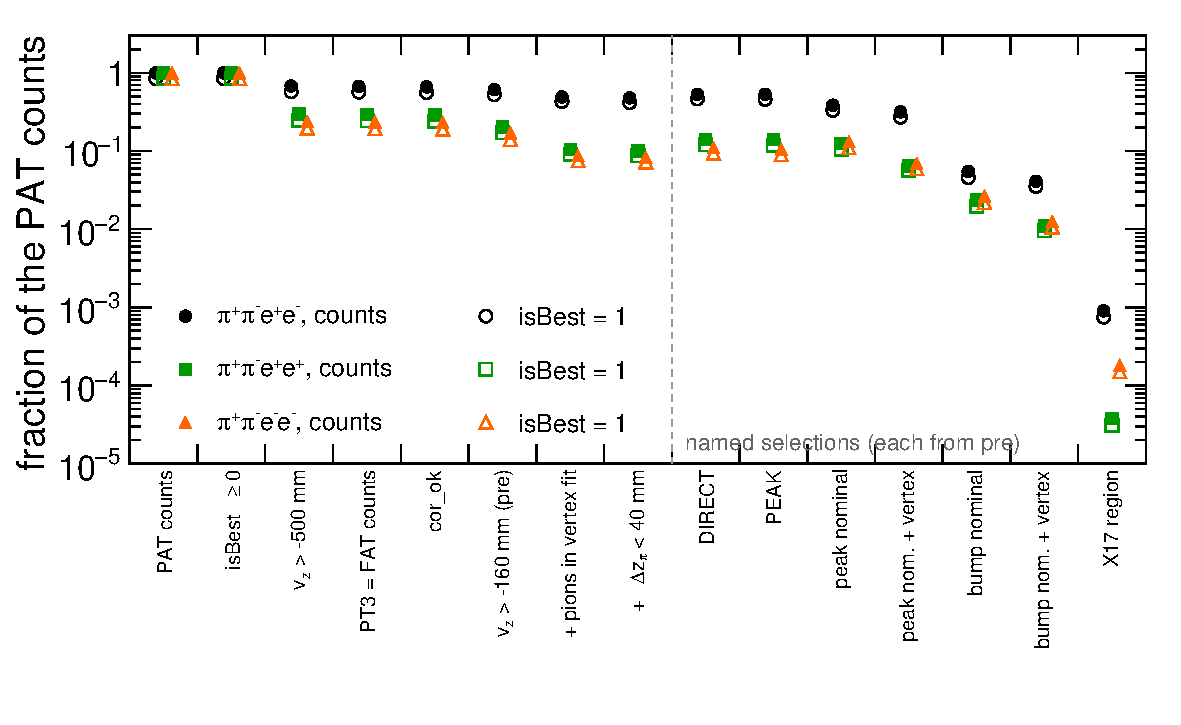
\includegraphics[width=\textwidth]{figs_exp/smp_cutflow_cnt.pdf}
\caption{Fraction of the PAT counts that remains after each step, for \pipi\ee (black circles), \pipi$e^+e^+$ (green squares)
and \pipi$e^-e^-$ (orange triangles; the like-sign colour key of the whole report). Selection: data, 29 PAT day files (PAT identification by \betanew: pions $3\sigma$, leptons $5\sigma$ with a RICH ring). Left of the dashed line, cumulative steps: all PAT counts; isBest $\ge0$; event vertex $\vz>-500$\,mm; PT3 (trigger bit 8192) $=$ FAT counts; corrected momenta of all four tracks; $\vz>-160$\,mm $=$ ``pre''; both pions in the event-vertex fit; both pion tracks within 40\,mm of the vertex along the beam ($\dzpi<40$\,mm). Right of it, the named selections, each on ``pre'': DIRECT ($\dzpi<40$\,mm); PEAK (also $\MMfour<2.85$\,\GeVcc); peak nominal (lab angle between \pipi and \ee $\alab<55^\circ$, $\Mpipi>0.30$\,\GeVcc) and + pion-vertex fit; bump nominal ($\alab<40^\circ$, $0.30<\Mpipi<0.41$\,\GeVcc) and + pion-vertex fit; X17 band in the frozen simulation window (pion-vertex fit, $15.5\le\Mee<24.5$\,\MeVcc, $0.5333\le\Mfour<0.5587$\,\GeVcc). Full markers: all stored combinations (isBest $\ge0$); open markers: best
combination only (isBest $=1$), also divided by \emph{all} PAT counts of the hypothesis (so they start at
0.84--0.86, the share of best-ranked combinations). Counts, not normalised to luminosity (notation: Table~\ref{tab:notation}).}
\label{fig:smp_cutflow}
\end{figure}

\begin{figure}[!htbp]
\centering
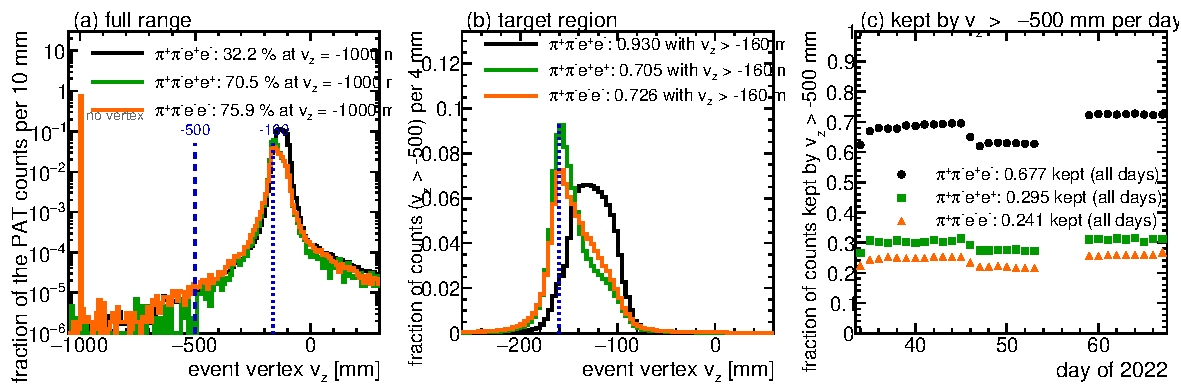
\includegraphics[width=\textwidth]{figs_exp/smp_vertex_cut_cnt.pdf}
\caption{Event-vertex position of the PAT counts of the three hypotheses (\pipi\ee black, \pipi$e^+e^+$ green,
\pipi$e^-e^-$ orange), all 29 days, all stored combinations (isBest $\ge0$), before any FAT cut. Selection: data, all 29 PAT day files; only the particle identification of PAT (\betanew; pions within $3\sigma$, leptons within $5\sigma$; leptons with a RICH ring) and all stored combinations (isBest $\ge0$); no trigger condition, no momentum-correction requirement, all \Mfour. (a) all counts; (b) the counts with a reconstructed event vertex ($\vz>-500$\,mm); (c) the share of all counts with $\vz>-500$\,mm, per day.
Panels from left to right: (a) full range, counts per 10\,mm normalised to all counts, log scale (Fig.~\ref{fig:spec_vz500}(a) shows the
same with 5\,mm bins, normalised per mm): the spike at $\vz=-1000$\,mm marks
events without a reconstructed vertex (32\,\% of the unlike-sign, 71\,\%/76\,\% of the like-sign counts);
dashed: the cuts $\vz>-500$\,mm (FAT) and $\vz>-160$\,mm (analysis). (b) Target region, counts per 4\,mm,
normalised to the counts with $\vz>-500$\,mm: the like-sign counts peak at $-158$\,mm, at the cut; the
unlike-sign counts follow the target (mode $-131$\,mm). (c) Fraction kept by $\vz>-500$\,mm per day. Counts, not
normalised to luminosity.}
\label{fig:smp_vertex}
\end{figure}

\begin{figure}[!htbp]
\centering
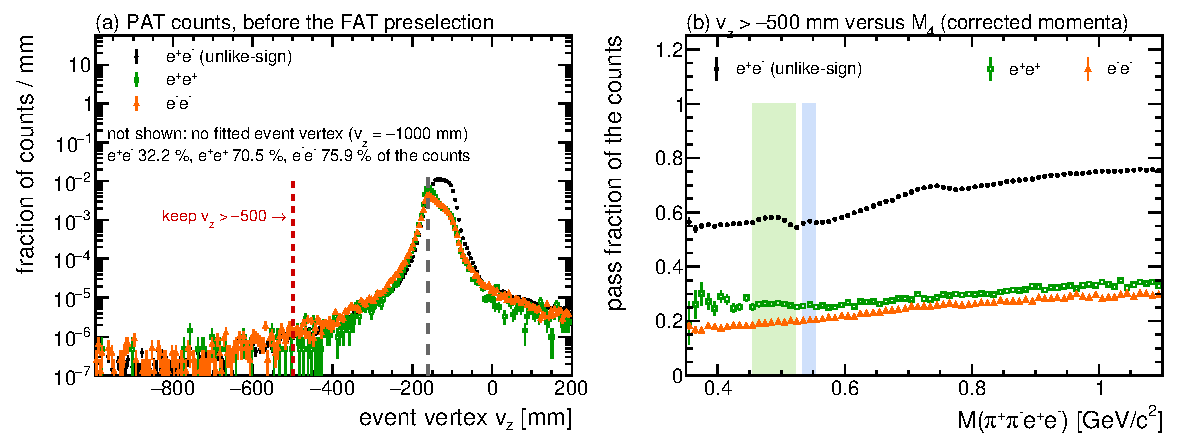
\includegraphics[width=\textwidth]{figs_exp/spec_vz500_cnt.pdf}
\caption{The mandatory FAT cut $\vz>-500$\,mm measured on the 29 PAT day files (all stored combinations,
isBest $\ge0$, before the FAT preselection). Selection: data, all 29 PAT day files; only the particle identification of PAT (\betanew) and all stored combinations (isBest $\ge0$); no trigger condition. (a) all counts, all \Mfour; (b) only the counts with energy-loss-corrected momenta of all four tracks (needed for \Mfour): their share with $\vz>-500$\,mm per 10\,\MeVcc bin of \Mfour, no trigger condition, no target-region cut. (a) \code{eVertReco_z} of the three hypotheses as a fraction of
\emph{all} counts of the sample per mm (5\,mm bins); the counts without a fitted vertex ($z=-1000$\,mm: 32.2\,\%
of \ee, 70.5\,\% of $e^+e^+$, 75.9\,\% of $e^-e^-$) count in the normalisation but are not drawn, so the
curves have areas 0.68, 0.30 and 0.24; red: the cut $-500$\,mm, grey dashed: the analysis cut $-160$\,mm.
(b) Pass fraction of the counts of $\vz>-500$\,mm against \Mfour, computed with the corrected momenta as in FAT
(\code{cor_ok} counts, 10\,\MeVcc bins; errors with the event-group correlation). Not normalised to
luminosity.}
\label{fig:spec_vz500}
\end{figure}

\subsection{Rates per day and the sector-2 deficit}
\label{sec:rates}
\textbf{Procedure.} For each day the number of counts of ``pre'' is multiplied by $64/63$ and divided by \Lan
of the day: $R$ in counts per \nbinv. The error combines the counts (with the event-group correlation) and the
statistical error of the daily luminosity. The mean is $\langle R\rangle=\sum(\text{counts}\times64/63)/\sum L$
(the maximum-likelihood constant); a $\chi^2$ tests the constancy over the 29 days.

\textbf{Result} (Fig.~\ref{fig:smp_rates}): $\langle R\rangle=739.17\pm0.42$ (\ee),
$14.358\pm0.058$ ($e^+e^+$) and $44.68\pm0.11$ ($e^-e^-$) counts per \nbinv (isBest $=1$: 632.08, 12.09,
36.79). The rates are \emph{not} constant within the statistics: rms 4.9\,\%, 14.1\,\% and 12.8\,\%,
$\chi^2/\mathrm{ndf}=7206/28$, 1185/28, 2781/28. They change in steps: flat on days 034--045 (\ee
0.95--1.04 of the mean), higher on 046--053 (\ee $+3.5$\dots$+10$\,\%, like-sign $+12$\dots$+25$\,\%), lower
on 059--067 (\ee $-3$\dots$-8$\,\%, like-sign $-13$\dots$-22$\,\%). The like-sign share
$(N_{++}+N_{--})/N$ per day has an rms of 8.5\,\% (ratio of the sums 0.0799), so the CB share depends on the
run conditions; the CB is therefore always formed on the summed sample. Dividing $R$ by $f_{\mathrm{LF}}$ of
the day does not make it flatter (rms 4.88\,\% $\to$ 4.83\,\% for \ee); the correlations of $R$ with
$f_{\mathrm{LF}}$ (+0.19/+0.24/+0.19) are not significant with 29 days. The cause is not proven; the event-vertex survival of the counts
changes in the same steps, but that is the share of non-target background counts: the $\eta$ efficiency of the vertex cut is consistent with
1 in every period within 1.7$\sigma$ ($\varepsilon_T$, \S\ref{sec:vtxeff}). \textbf{The steps follow the beam halo} (an indication found
after the first draft, \S\ref{sec:walls}): the counts in front of the cell ($-200\le\vz<-170$\,mm) measure the halo, and their rate per
luminosity steps on the same days (up from day 046, down from day 059). A per-day fit of $R$ with the halo level lowers the day-to-day rms from
4.9 to 1.7\,\% (like-sign counts: from 13 to 2.9\,\%). A per-day yield per luminosity therefore has a
systematic scatter of about 5\,\%, and the integrated yield carries a period-normalisation uncertainty of $\pm5$\,\% until the cause of the
steps is confirmed (Table~\ref{tab:syst}). The $\eta$ peak per luminosity is constant within
its 16\,\% precision per period (\S\ref{sec:stab}).

\textbf{Sector 2.} Table~\ref{tab:smp_sectors} and Fig.~\ref{fig:smp_sectors} give the share of the tracks
per sector. On days 034--044 the sector-2 share of the leptons is 0.1669, against 0.1771 on 045--067; the
pions show the same (0.1610 against 0.163--0.167). Day 045 is also low (leptons 0.161, pions 0.159), although
the luminosity files assign the deficit only to days 034--044. The like-sign samples show the same pattern. The elastic events of day 045
have no sector-2 deficit in PT2 or PT3 (1.074, see the PT2 check below), so the luminosity of day 045 needs no sector-2 correction; the
low sector-2 share of the lepton channel on day 045 is specific to it (its cause was not studied).

\textbf{Later details (Part~III, package WP2; data only).} The sector numbering $(\lfloor\varphi/60^\circ\rfloor+5)\bmod6$ was verified on
the acceptance gaps of the lepton tracks, and the deficit lies exactly in $\varphi=180$--$240^\circ$. In blocks of 25\,\nbinv it is
intermittent: 30 blocks of days 034--045 lie more than $4\sigma$ below 1 (down to 0.58), and only one block elsewhere (day 061). Day 045
still has three deficit blocks (00:00--02:07, 02:08--04:05 and 07:27--17:56; day efficiency $0.903\pm0.007$), day 046 none ($1.008\pm0.007$):
this confirms that day 045 is low. As a double ratio (counts with a sector-2 track against counts without, deficit days against clean days)
the efficiency is $\varepsilon_{s2}=0.9266\pm0.0024$ for 034--045 against 046--067 (single early/late ratio $0.9538\pm0.0017$ for 034--044 against
045--067, on ``pre'' + vertex). With the simulated share of the $\eta$ signal that uses a sector-2 track, Part~III corrects its $\eta$ yields
by $C_{\mathrm{sec}}=1.0110\pm0.0035$ (peak 1.0116, bump 1.0104; period I alone 1.023--1.025), in line with the $+1.2$ to $+1.4$\,\% of all counts
below (Fig.~\ref{fig:walls_vz}a, b in \S\ref{sec:walls}).
The span 034--045 of $C_{\mathrm{sec}}$ was approved by the analyst on 15 November 2026 (Part~III, D26).


\textbf{Estimate of the lost counts.} The fraction $f_{\mathrm{ref}}$ of counts with at least one track in sector 2 is
taken from the reference days. Counts without a sector-2 track are assumed unaffected. The expected number of
sector-2 counts on the deficit days is $f_{\mathrm{ref}}/(1-f_{\mathrm{ref}})$ times the counts without a
sector-2 track, and the loss is (expected $-$ observed)/(counts + expected $-$ observed). For the \ee counts,
0.4448 against 0.4616 gives a loss of 3.0\,\% on days 034--044 (3.3\,\% for 034--045 against 046--067;
like-sign 3.1--3.7\,\%), that is 1.2\,\% (1.4\,\%) of the whole sample. It is not in $L$, not corrected,
and belongs to the trigger-efficiency uncertainty. It is not visible in the total \ee rate (ratio
034--044/045--067 $=0.992$) because the day-to-day scatter is larger.

\begin{figure}[!htbp]
\centering
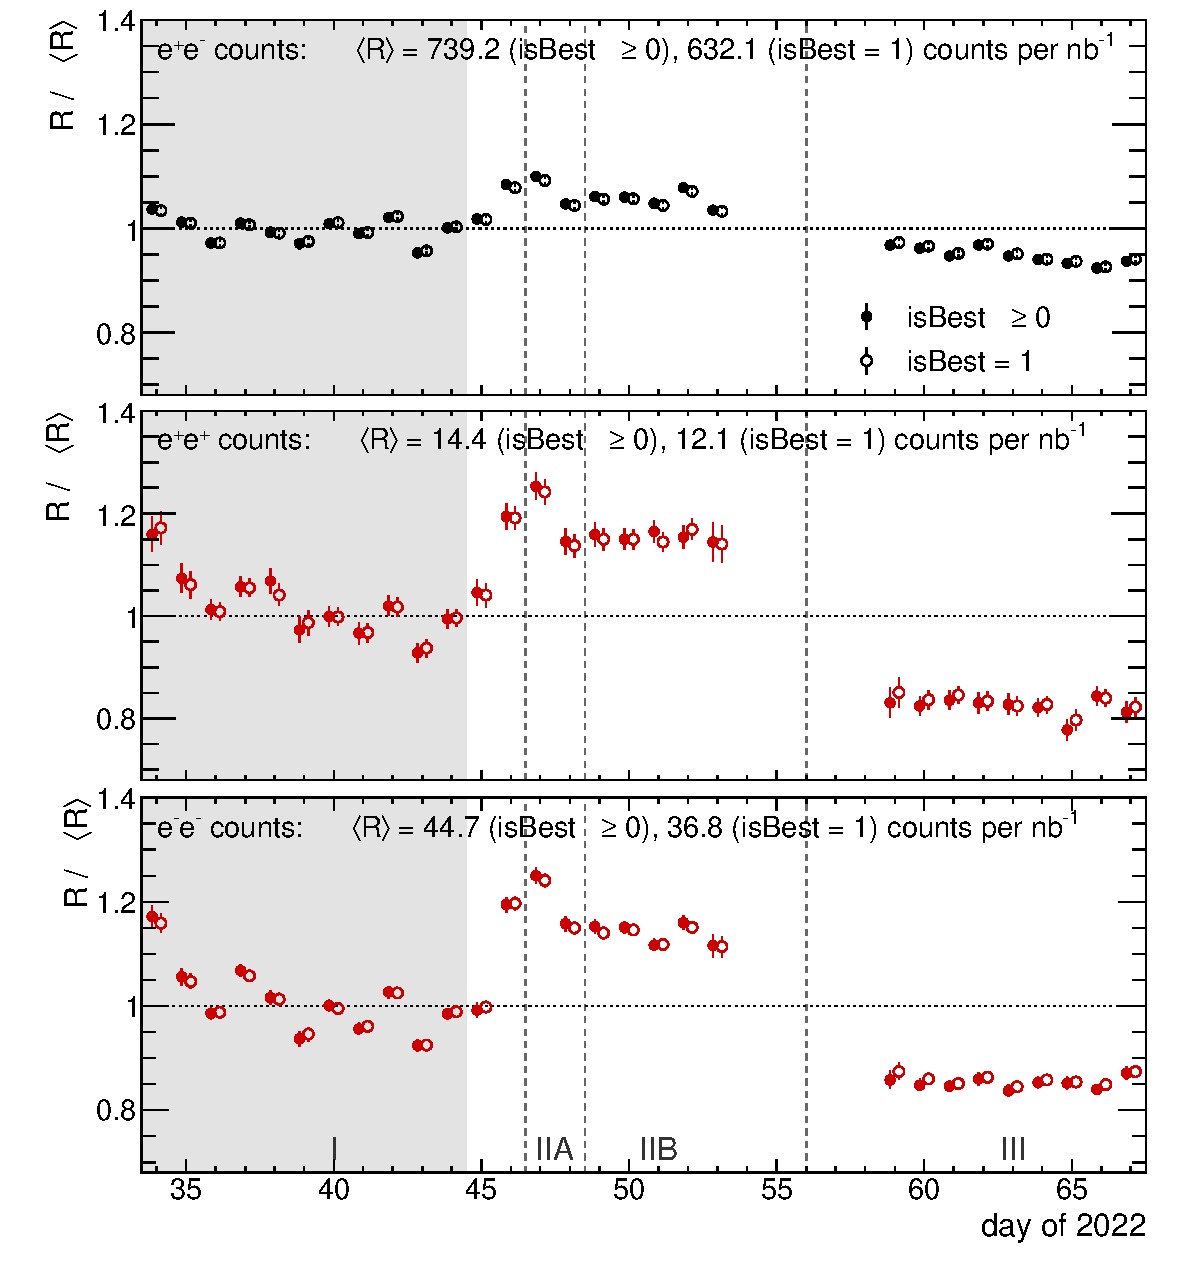
\includegraphics[width=0.92\textwidth]{figs_exp/smp_rates_perday_cnt.pdf}
\caption{Visible rate per day, $R=\text{counts}\times\frac{64}{63}/L$, relative to the luminosity-weighted
mean $\langle R\rangle$, for \ee (top), $e^+e^+$ (middle) and $e^-e^-$ counts (bottom). Selection: data; \ptthreecap{}, event vertex in the target region ($\vz>-160$\,mm), particles identified by their START-free velocity \betanew (pions within $3\sigma$, leptons within $5\sigma$ of their band; leptons with a RICH ring, pions without), energy-loss-corrected momenta of all four tracks (\code{cor_ok} $=1$) (``pre''; FAT: $\vz>-500$\,mm, PT3), all \Mfour, \Mee and \Mpipi, per day; full markers: all stored combinations (isBest $\ge0$); open markers: only the best-ranked combination of each event (isBest $=1$); unlike-sign and like-sign counts with the same cuts, no CB subtracted. $L$ = START-free luminosity of the analysed runs of the day; error bars: statistics with
the event-group correlation. Grey: days 034--044 with the sector-2 trigger deficit (not in $L$); dashed
lines: period boundaries. The means in counts per \nbinv are printed; $\chi^2/\mathrm{ndf}$ of a constant
7206/28, 1185/28, 2781/28.}
\label{fig:smp_rates}
\end{figure}

% smp_sectors_cnt.tex: copy of smp_sectors.tex with "rows" -> "counts" (analyst, 15 Nov 2026; Part II writer, integ4)
% smp_sectors.tex -- written by plots/exp_report/smp_flow.C (numbers: tables_exp/smp_sectors.txt)
\begin{table}[H]
\centering\small
\setlength{\tabcolsep}{4pt}
\caption{Share of the tracks per sector (in \%) in the $e^+e^-$ counts of the selection pre (all stored combinations, isBest $\geq 0$, corrected momenta, PT3, $v_z>-160$~mm), for the two lepton slots and the two pion slots. Days 034--044 carry the sector-2 hardware trigger deficit, which is not contained in the luminosity. Binomial errors on the track counts are 0.02--0.1 percentage points.}
\label{tab:smp_sectors}
\begin{tabular}{llrrrrrr}
\toprule
Days & Tracks & S0 & S1 & S2 & S3 & S4 & S5 \\
\midrule
034-044 & leptons & 14.73 & 18.73 & 16.69 & 18.31 & 17.39 & 14.15 \\
045-046 & leptons & 14.76 & 18.30 & 17.12 & 18.19 & 17.32 & 14.31 \\
IIA & leptons & 14.84 & 17.72 & 18.09 & 18.17 & 16.97 & 14.20 \\
IIB & leptons & 14.97 & 17.97 & 17.75 & 18.01 & 16.94 & 14.37 \\
III & leptons & 14.83 & 18.27 & 17.73 & 17.91 & 16.99 & 14.27 \\
all & leptons & 14.81 & 18.36 & 17.31 & 18.12 & 17.16 & 14.24 \\
\midrule
034-044 & pions & 16.73 & 16.99 & 16.10 & 16.82 & 16.63 & 16.74 \\
045-046 & pions & 16.59 & 16.85 & 16.33 & 16.65 & 16.96 & 16.62 \\
IIA & pions & 16.71 & 16.59 & 16.58 & 16.53 & 16.92 & 16.66 \\
IIB & pions & 16.62 & 16.76 & 16.59 & 16.38 & 16.90 & 16.75 \\
III & pions & 16.52 & 16.83 & 16.65 & 16.35 & 16.86 & 16.79 \\
all & pions & 16.64 & 16.87 & 16.39 & 16.57 & 16.79 & 16.74 \\
\bottomrule
\end{tabular}
\end{table}


\begin{figure}[!htbp]
\centering
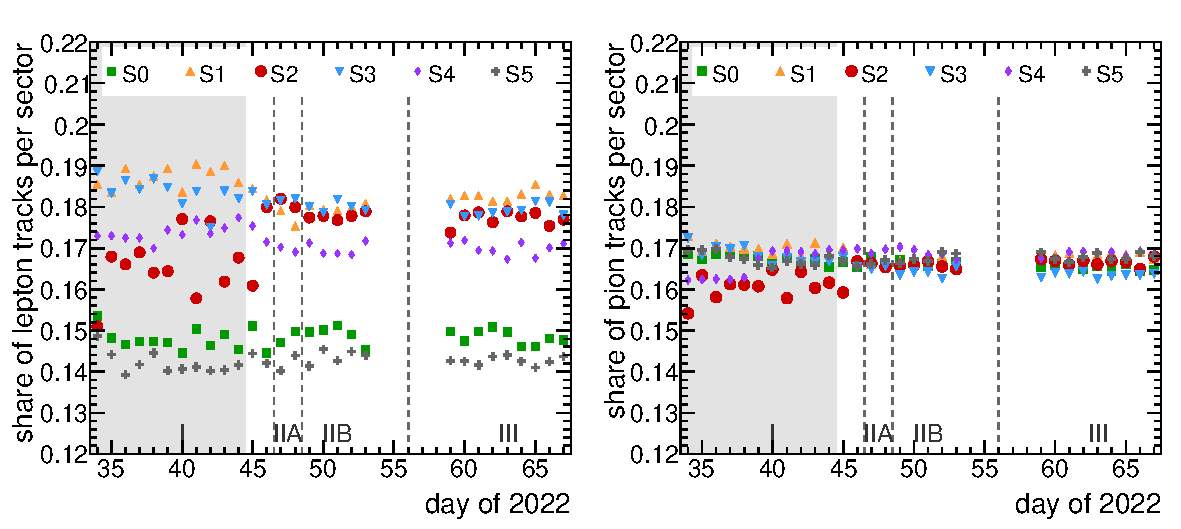
\includegraphics[width=\textwidth]{figs_exp/smp_sectors.pdf}
\caption{Share of the lepton tracks (left) and the pion tracks (right) per sector and day, \ee counts of the
selection ``pre'', all combinations (isBest $\ge0$). Selection: data; \ee counts of the base cuts: \ptthreecap{}, event vertex in the target region ($\vz>-160$\,mm), particles identified by their START-free velocity \betanew (pions within $3\sigma$, leptons within $5\sigma$ of their band; leptons with a RICH ring, pions without), energy-loss-corrected momenta of all four tracks (\code{cor_ok} $=1$), all stored \ppee combinations of each event (isBest $\ge0$) (``pre''), all \Mfour, \Mee and \Mpipi; each of the four tracks of a count assigned to its sector. Grey: days 034--044 (sector-2 hardware trigger deficit,
not in $L$). The sector-2 share (red circles) is low on these days and also on day 045. Track shares, no
luminosity normalisation.}
\label{fig:smp_sectors}
\end{figure}

\textbf{Sector 2 in the elastic events: the PT2 check} (added on 15 November 2026; data only). \emph{In short: on days 041--044 the elastic
events lose sector-2 triggers in PT2, on day 045 they do not, so $L$ is right on day 045 and the day-045 deficit of our counts belongs to the
lepton channel.} \emph{Source:} the analyst's luminosity table \code{s2_trigger_perday.csv}, the number of elastic events per sector and day
for the triggers PT2 (from which $L$ is made) and PT3. \emph{Definition:} for each day, the sector-2 count divided by the mean count of the
other five sectors, and this ratio divided by the same ratio summed over the clean days 046--067 (1 means no deficit). \emph{Result}
(Table~\ref{tab:s2pt2}): on days 041--044 sector~2 has only 0.65--0.76 of its clean-day share of the elastic PT2 events (0.92--0.98 in PT3);
on day 045 it has $1.074\pm0.009$ in PT2 and $1.074\pm0.008$ in PT3, as on day 046 (1.087, 1.098). \emph{What was expected:} if the
hardware deficit of days 034--044 had continued into day 045, the elastic events of that day would show it too. \emph{Meaning:} the elastic
events of day 045 show no sector-2 deficit, so the luminosity without a sector-2 correction on day 045 is right and $L=6079.2\,\nbinv$ is
unchanged. The deficit of the \ppee counts on day 045 (sector-2 efficiency $0.903\pm0.007$, in the periods 0:00--2:07, 2:08--4:05 and
7:27--17:56 of the day) is specific to the lepton channel; its cause was not studied. The same table also shows the PT2 deficit on days
034--040 (0.45--0.73 by the same definition, recomputed here). A recomputation of the analyst's numbers from the table (ratio of the summed
counts) agrees within 0.002.

\begin{table}[H]
\centering
\caption{\textbf{Sector 2 in the elastic events, PT2 and PT3}, days 041--047 (the analyst's luminosity table \code{s2_trigger_perday.csv}):
elastic events in sector~2 over the mean of the other five sectors, divided by the same ratio over the clean days 046--067 (1 $=$ no
deficit). Values as given by the analyst; errors statistical (counts), for days 042--044, 046 and 047 recomputed from the table. For comparison, the
sector-2 efficiency of the \ppee counts on day 045 is $0.903\pm0.007$ (Part~III, WP2).}
\label{tab:s2pt2}
\footnotesize
\setlength{\tabcolsep}{4pt}
\begin{tabular}{@{}lccccccc@{}}
\toprule
day & 041 & 042 & 043 & 044 & 045 & 046 & 047 \\
\midrule
PT2 & $0.654\pm0.006$ & $0.762\pm0.006$ & $0.688\pm0.006$ & $0.753\pm0.006$ & $\mathbf{1.074\pm0.009}$ & $1.087\pm0.009$ & $1.005\pm0.009$ \\
PT3 & $0.915\pm0.007$ & $0.981\pm0.007$ & $0.941\pm0.007$ & $0.983\pm0.007$ & $\mathbf{1.074\pm0.008}$ & $1.098\pm0.009$ & $1.010\pm0.008$ \\
\bottomrule
\end{tabular}
\end{table}

\subsection{Target walls: the empty-target runs}
\label{sec:walls}
\textbf{Why.} $L$ counts reactions in the liquid hydrogen only, and the luminosity files ask for an empty-target subtraction (rule 4 of
\S\ref{sec:lumi}). The production of this report holds no empty-target runs, so the first draft could not give the size of the
contribution of the target walls (the Mylar windows of the cell and the material around it). Part~III (package WP2) found the
empty-target runs and processed them with the programs and the selection of this report; two independent verifiers checked it, one
(vw2a) by reproducing every number with own code, the other (vw2b) by auditing the method. Everything in this subsection is measured from
the data, except where the simulation is named. Notes: \code{docs/latex/notes_all/wp2_results.md} (sections 1.3, 2.2 and 7) and
\code{docs/latex/notes_all/verify_wp2/}.

\textbf{Procedure.}
\begin{enumerate}\setlength{\itemsep}{0pt}
\item \textbf{Runs.} Empty-target DSTs exist for the days 034 (7 runs, 70 DSTs), 047 (16 runs, 160 DSTs) and 065 (104 runs, 1040 DSTs):
      127 runs, 1270 DSTs. These are the days that the luminosity analysis used for its own correction of the elastic events from the
      target windows.
\item \textbf{PAT} was rebuilt from the production tag \code{prod-feb22-betanew-2026-10-28} (sources identical to the tag, the same PID
      file) and run on the 1270 DSTs (44 jobs, all successful). Check of the build: one full-target DST processed with it gives exactly the
      production entries (38 of 38 \code{PipPimEpEm_ID} and 764 of 764 \code{EpEm_ID} entries of \code{lep_034}).
\item \textbf{FAT} ran with the data configuration of this report ($T_{\mathrm{beam}}=4530$\,MeV, PT3, $\vz>-500$\,mm, corrected momenta),
      and the compact file was made with a copy of \code{scan_prepare.C} in which only the paths differ: 31\,479 \ee, 2\,250 $e^+e^+$ and
      6\,196 $e^-e^-$ counts.
\item \textbf{Flux normaliser $b$.} An empty run has no hydrogen luminosity, so its beam flux is measured with counts that both kinds of
      runs have: the counts of the channel (\ee, $e^+e^+$ and $e^-e^-$; isBest $\ge0$, $\vz>-500$\,mm, PT3, \code{cor_ok}) with
      $-200\le\vz<-170$\,mm, in front of the cell. They come from beam halo on the structures there: 89--93\,\% of them cross 8\,mm or more
      from the beam axis, their like-sign/unlike-sign ratio is the same in empty and full runs (0.459 against 0.455), and they hold no
      hydrogen counts (in the simulation the LH$_2$ cell puts $1.7\times10^{-5}$ of its simulated entries there; in the data the pion-vertex fraction allows
      at most about 2\,\%). $b=U_{\mathrm{full}}/U_{\mathrm{empty}}$ of the same day is $10.35\pm0.79$ (034), $15.44\pm0.95$ (047) and
      $0.932\pm0.030$ (065). A fit of the \vz profile (simulated LH$_2$ + empty target) gives 0.85--0.90 of $b$, and positivity of
      full $-$ $b\times$empty in the entrance-window bin allows at most 1.06--1.22 $b$: for day 065, which dominates, $-12/+6$\,\% of the share.
\item \textbf{Share} $\fwin=b\,Y_{\mathrm{empty}}/Y_{\mathrm{full}}$ for each selection, window and quantity; the three days are combined
      with the luminosity of the period each day represents (034 $\to$ I, 047 $\to$ IIA + IIB, 065 $\to$ III), with event-group errors of
      both samples.
\end{enumerate}

\begin{figure}[tbp]
\centering
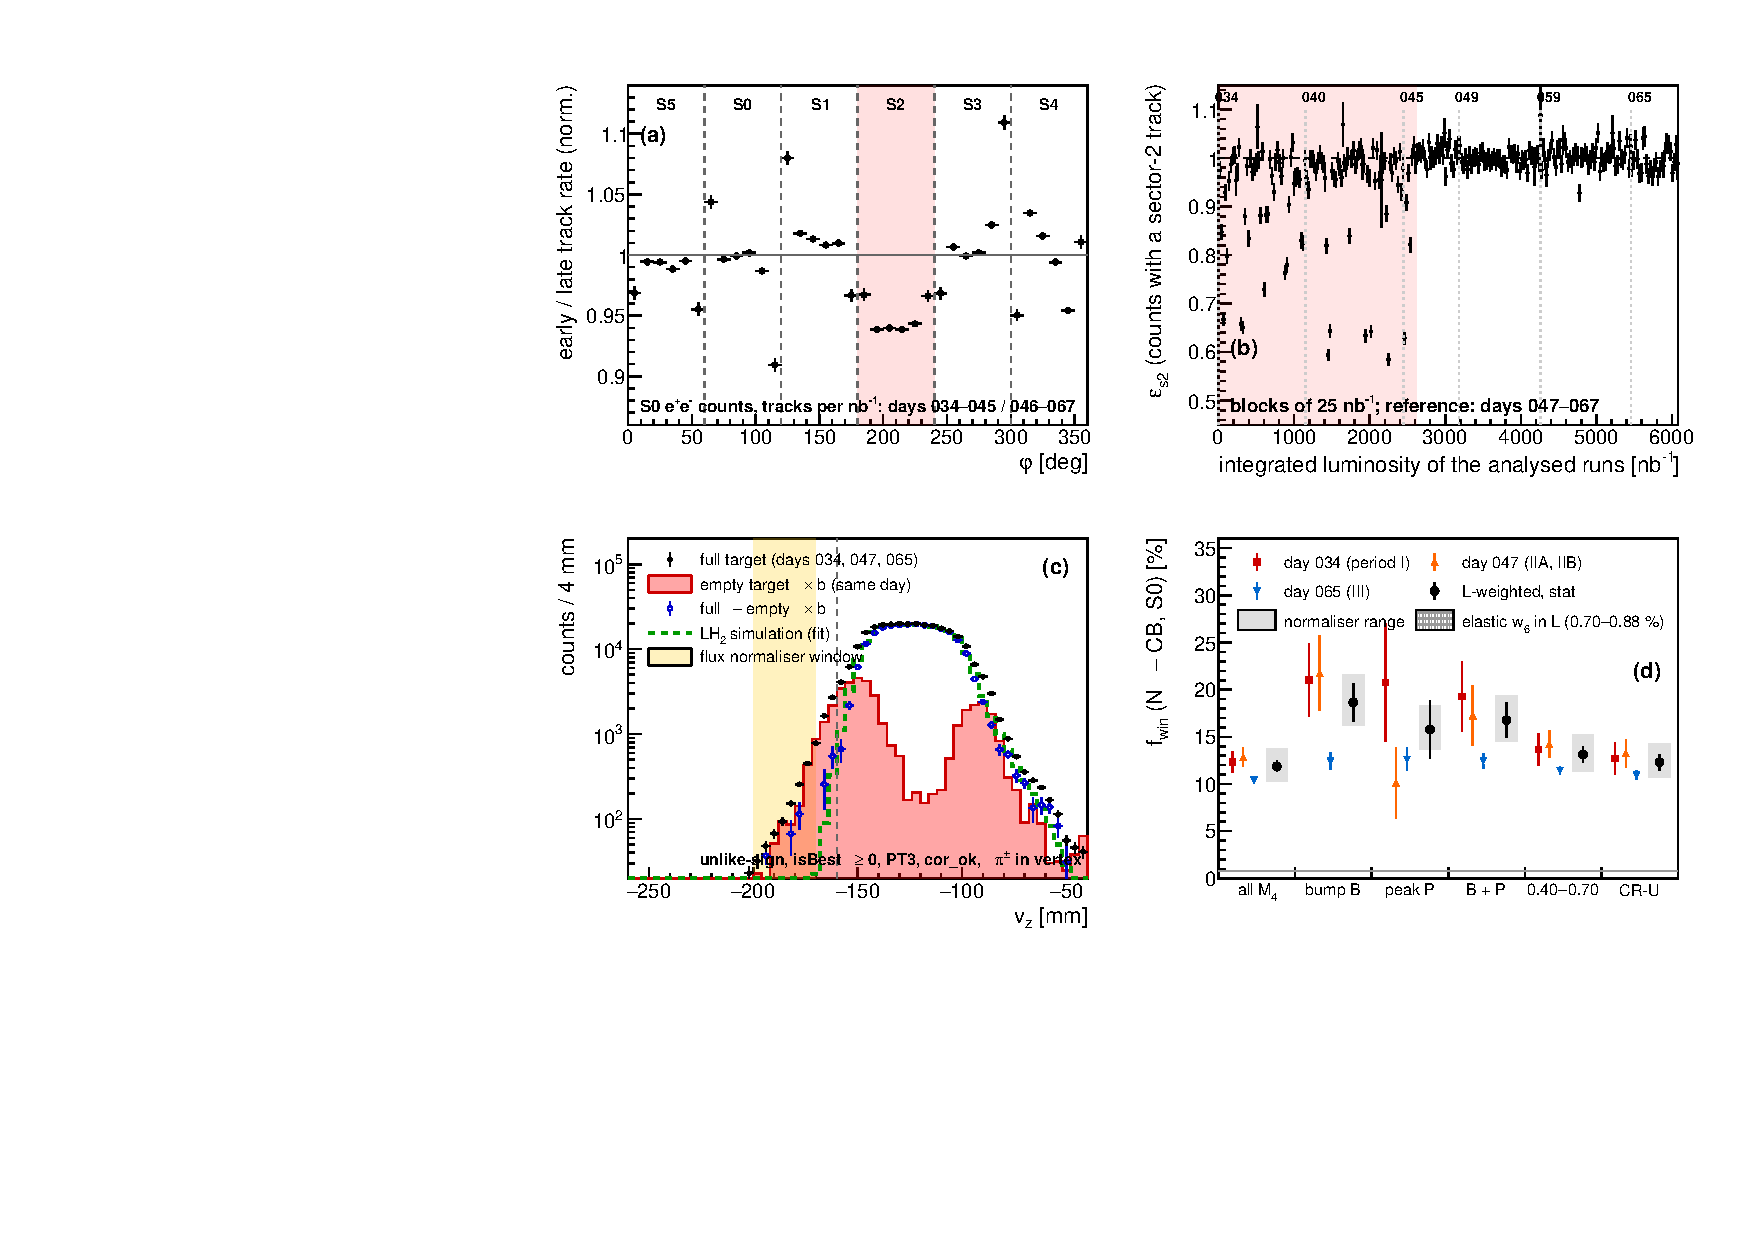
\includegraphics[width=0.86\textwidth]{figs_all/wp2_N1v2_cnt.pdf}
\caption{\textbf{What it shows: the sector-2 deficit is intermittent and sits in sector 2 only (top); the target walls give a visible part of
the counts (bottom).} Selection: data (the green curve in (c) is the LH$_2$ simulation). All panels: \ee counts with \ptthreecap{}, the \betanew particle identification, energy-loss-corrected momenta of all four tracks, all stored combinations (isBest $\ge0$) and both pions used in the event-vertex fit, all \Mfour. (a), (b), (d): also the target-region cut $\vz>-160$\,mm (``pre'' + vertex); (a) all four tracks of each count, days 034--045 against 046--067; (b) counts with at least one track in sector~2 against counts without one, per block of 25\,\nbinv, reference days 047--067; (d) $N-\mathrm{CB}$ in the \Mfour windows: all \Mfour, bump window 0.4550--0.5225, peak window 0.53364--0.55416, the two together, 0.40--0.70 and the upper control region 0.565--0.70\,\GeVcc (CR-U). (c) no target-region cut (a reconstructed event vertex, $\vz>-500$\,mm; the cut at $-160$\,mm is drawn), days 034 + 047 + 065; empty target scaled with the \ee and like-sign counts in $-200\le\vz<-170$\,mm (no pion-vertex requirement there). Part~III, WP2; data only except the green curve in (c), which is the LH$_2$ simulation. (a) Track rate per \nbinv of the
\ee counts of ``pre'' + vertex (isBest $\ge0$), days 034--045 divided by days 046--067, per 10$^\circ$ of azimuth, normalised outside
180--240$^\circ$; the labels S0--S5 are the sector numbers. (b) $\varepsilon_{s2}$: counts with a sector-2 track relative to counts without one, per
block of 25\,\nbinv of the analysed runs, normalised to days 047--067; shaded: the deficit span 034--045. (c) Vertex $z$ of the unlike-sign counts
(isBest $\ge0$, PT3, \code{cor_ok}, both pions in the vertex fit, all \Mfour), days 034 + 047 + 065: full target (black), empty target
$\times\,b$ (red; flux ratio of the same day from the counts in the shaded window $-200$ to $-170$\,mm), their difference (blue), LH$_2$
\emph{simulation} fitted to the full-target profile (green, dotted); dashed: the cut $\vz>-160$\,mm. (d) \fwin, the wall share of
$N-\mathrm{CB}$ of ``pre'' + vertex per \Mfour window, per empty-target day and luminosity-weighted (statistical errors; before the halo
correction); grey boxes: range of the flux ratio; hatched: the elastic window share $w_6$ already removed from $L$ (0.70--0.88\,\%). Counts, not
normalised to luminosity except (a).}
\label{fig:walls_vz}
\end{figure}

\begin{figure}[tbp]
\centering
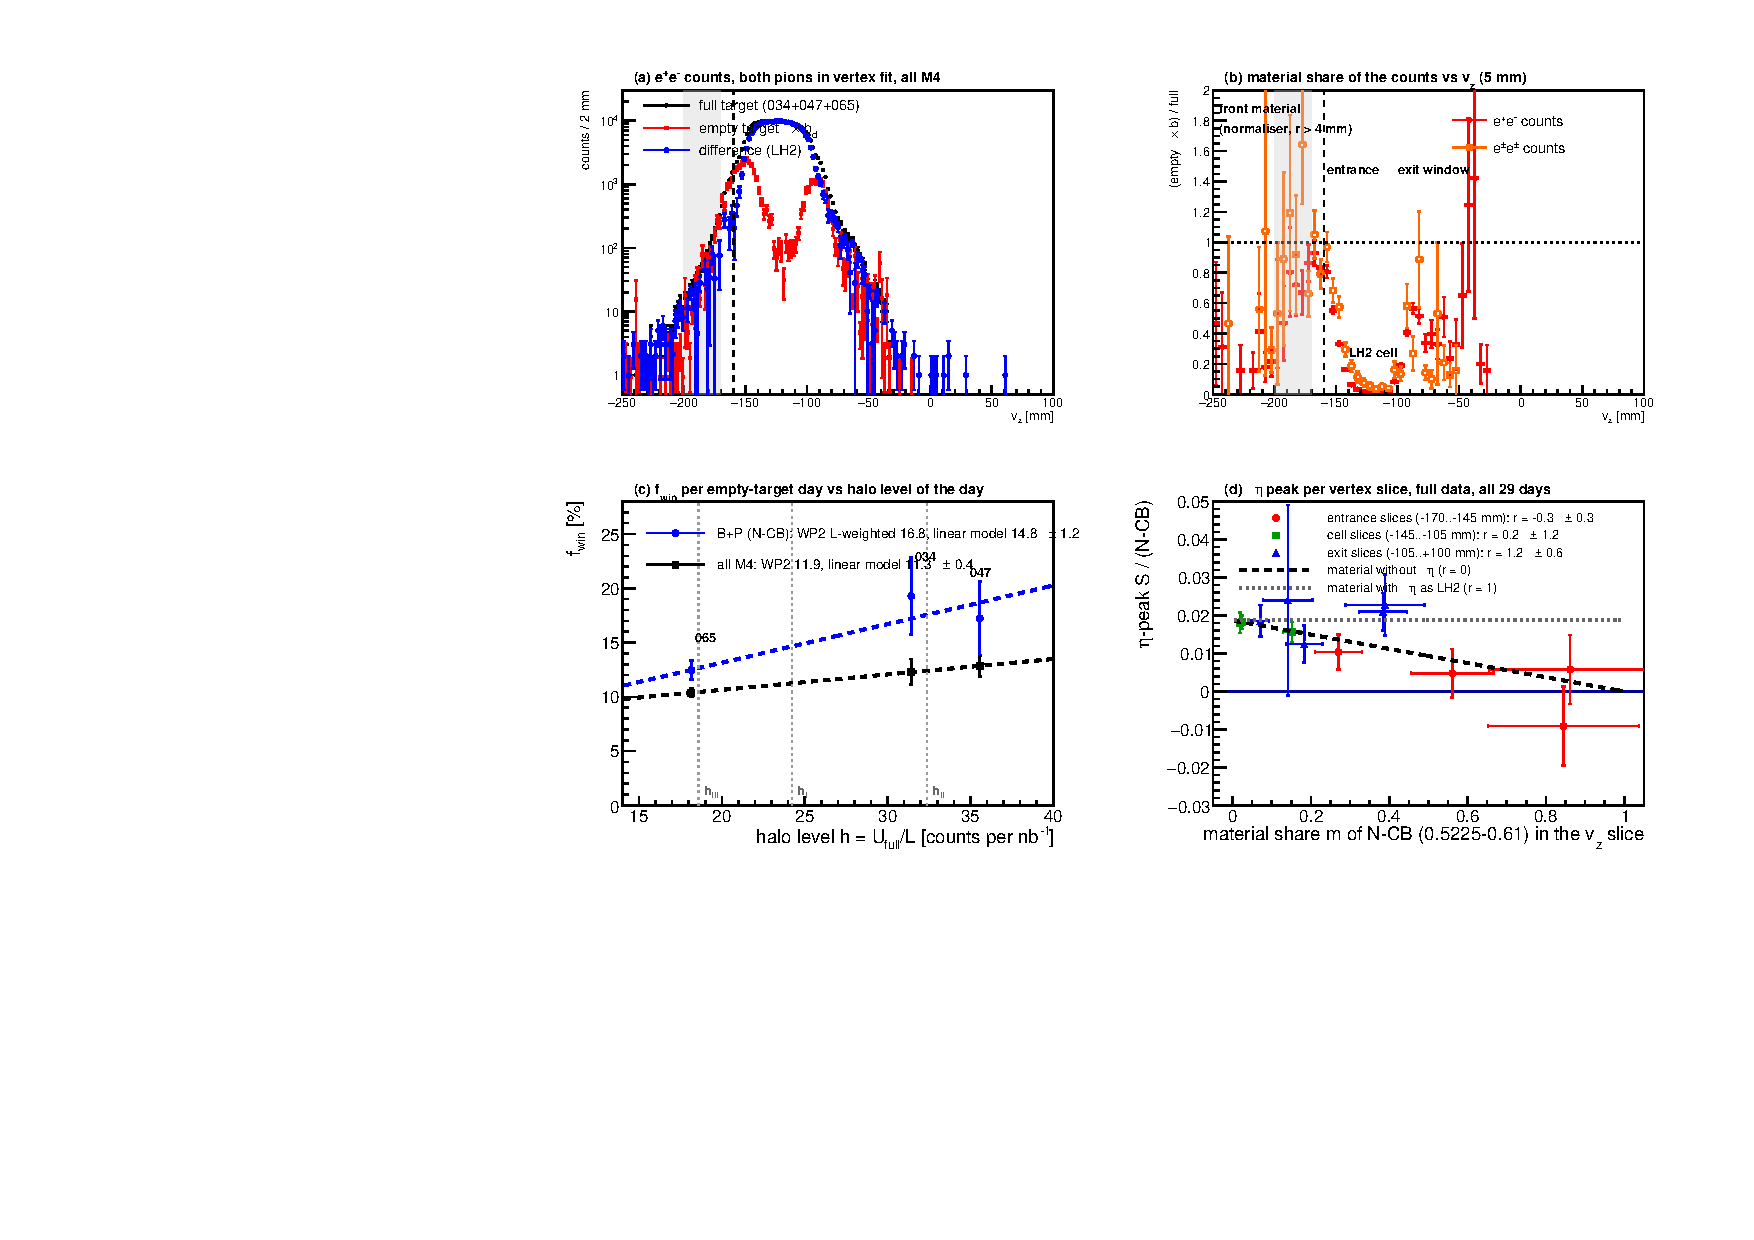
\includegraphics[width=0.86\textwidth]{figs_all/vw2a_fig_cnt.pdf}
\caption{\textbf{What it shows: the $\eta$ signal does not come from the target walls.} Selection: data only. All panels: isBest $\ge0$, a reconstructed event vertex ($\vz>-500$\,mm), \ptthreecap{}, the \betanew particle identification, energy-loss-corrected momenta of all four tracks, both pions used in the event-vertex fit, all \Mfour. (a), (b): days 034 + 047 + 065, no target-region cut (the cut $\vz>-160$\,mm is drawn); (a) \ee counts; (b) \ee and like-sign counts; the empty-target runs scaled with the flux ratio of the same day, from the \ee and like-sign counts with $-200\le\vz<-170$\,mm in front of the cell (no pion-vertex requirement there). (c) with the target-region cut $\vz>-160$\,mm (``pre'' + vertex); $N-\mathrm{CB}$ in all \Mfour and in the bump and peak windows together (0.4550--0.5225 and 0.53364--0.55416\,\GeVcc). (d) full-target runs of all 29 days, no target-region cut, 12 slices of \vz with the edges $-170$, $-160$, $-155$, $-150$, $-145$, $-135$, $-115$, $-105$, $-100$, $-95$, $-85$, $-60$ and $+100$\,mm; in each slice the $\eta$-peak content $S$ (fixed Gaussian plus second-order polynomial, 0.5225--0.61\,\GeVcc) divided by $N-\mathrm{CB}$ in the same range, CB $=2\sqrt{N_{++}N_{--}}$ of the slice, $k=1$. Figure of the independent verification vw2a of
Part~III; data only (full-target runs of all 29 days and the empty-target runs of days 034, 047, 065). (a) Vertex $z$ of the \ee counts
(``pre'' + both pions in the vertex fit, all \Mfour), days 034 + 047 + 065: full target (black), empty target scaled by the flux ratio $b_d$ of
the same day (red), their difference (blue). (b) Wall share of the counts per 5\,mm slice of \vz (\ee and like-sign counts): the walls dominate at
the entrance ($\approx-150$\,mm) and the exit window ($\approx-90$\,mm); inside the LH$_2$ cell they give about 1\,\%; grey: the
normaliser window. (c) \fwin per empty-target day against the halo level $U_{\mathrm{full}}/L$ of that day (B+P and all \Mfour, $N-\mathrm{CB}$):
the share follows the halo, and the empty-target days had a high halo; at the luminosity-weighted halo level the line drawn gives
$\fwin(\mathrm{B+P})=14.8\pm1.2$\,\% instead of 16.8\,\% (the halo correction of Table~\ref{tab:walls}, by vw2b: $14.7\pm1.1$\,\%). (d) $\eta$-peak content $S$ per $N-\mathrm{CB}$ count in each \vz slice of the full data,
all 29 days, against the material share of the slice (entrance, cell and exit slices). If the walls produced no $\eta$, the points would follow
the dashed line (zero at material share 1); if they produced $\eta$ like hydrogen, the dotted line. The entrance slices (red), where the walls
give 30--90\,\% of the counts, fall to about zero ($r=-0.27\pm0.34$ for these slices alone); the exit-window slices are consistent with
the hydrogen rate ($r=1.21\pm0.64$); the fit of all slices gives $r=0.07\pm0.30$, $f_\eta=3^{+4}_{-3}$\,\%. Counts, not normalised to luminosity.}
\label{fig:walls_feta}
\end{figure}

\begin{table}[H]
\centering
\caption{Share \fwin of the target walls in the counts, in per cent, from the empty-target runs of days 034, 047 and 065 (Part~III, WP2; reproduced
by the verifier vw2a; halo correction by vw2b). Data only. $N-\mathrm{CB}$ unless stated; isBest $\ge0$; flux normaliser from the counts with
$-200\le\vz<-170$\,mm; errors statistical (event groups). ``pre'' + vertex $=$ ``pre'' + both pions in the event-vertex fit (Part~III's S0).
Halo-corrected: each day scaled to the luminosity-weighted halo level of the beam time (computed for ``pre'' + vertex only; systematic
$^{+1.0}_{-2.0}$ for B+P and $^{+0.8}_{-1.5}$ for all \Mfour). Windows: B $=$ bump window 0.4550--0.5225, P $=$ peak window
0.53364--0.55416\,\GeVcc. These are shares of the \emph{counts}, mostly non-$\eta$ background; the share of the $\eta$ signal is
$f_\eta=3^{+4}_{-3}$\,\% (text). Sources: \code{tables_all/wp2_win_summary.txt}, \code{verify_wp2/vw2b_note.md}.}
\label{tab:walls}
\small
\begin{tabular}{@{}l r r r@{}}
\toprule
window & ``pre'' + vertex, raw & ``pre'' + vertex, halo-corrected & ``pre'', raw \\
\midrule
all \Mfour & $11.86\pm0.59$ & $11.29\pm0.37$ & $16.06\pm0.78$ \\
B & $18.64\pm2.04$ & $16.08\pm1.26$ & $21.68\pm2.52$ \\
P & $15.78\pm3.07$ & $12.64\pm1.47$ & $24.19\pm3.60$ \\
B + P & $16.76\pm1.88$ & $14.70\pm1.08$ & $22.44\pm2.21$ \\
0.40--0.70\,\GeVcc & $13.12\pm0.85$ & $12.45\pm0.52$ & $18.98\pm1.14$ \\
\midrule
$N$ (not $N-\mathrm{CB}$), all \Mfour & $12.79\pm0.60$ & -- & $18.85\pm0.85$ \\
like-sign counts, all \Mfour & $29.7\pm2.2$ & -- & $52.4\pm2.8$ \\
\bottomrule
\end{tabular}
\end{table}

\textbf{Result: share of the counts} (Table~\ref{tab:walls}, Fig.~\ref{fig:walls_vz}c, d). For ``pre'' + vertex the walls give 11.9\,\% of
all $N-\mathrm{CB}$ counts and 13.1\,\% in 0.40--0.70\,\GeVcc; for ``pre'' itself, without the pion-vertex requirement, which removes a part of the wall counts, 16.1\,\% and
19.0\,\%. The material spectrum is softer: for ``pre'' + vertex \fwin is 0.11--0.12 above 0.56\,\GeVcc and 0.15--0.25 below 0.52\,\GeVcc. The
walls are rich in CB: like-sign/unlike-sign is 0.21 in the empty-target counts against 0.084 in the full target ($\vz>-160$\,mm, ``pre''), so
they give about half of the like-sign counts of ``pre'' ($52\pm3$\,\%, raw). By vertex region (``pre'' + vertex, B + P): 6.6\,\% of
$N-\mathrm{CB}$ from $-160$\dots$-145$\,mm (entrance window), 5.9\,\% from $-145$\dots$-105$\,mm and 4.7\,\% from $-105$\,mm on (exit
windows); inside the cell itself the walls give only about 1\,\% of the counts, the rest are the window peaks smeared by the vertex resolution
(Fig.~\ref{fig:walls_feta}b). Per \vz slice of the unlike-sign counts of ``pre'' (all \Mfour, raw) the wall share is 1.01 in $-200$\dots$-170$\,mm
(the normaliser window, 1 by construction), 0.87 in $-170$\dots$-160$, 0.76 in $-160$\dots$-150$, 0.30 in $-150$\dots$-140$, 0.05 in
$-140$\dots$-110$ and 0.13 in $-110$\dots$-90$\,mm; 0.19 for all $\vz>-160$\,mm (0.28 in P). The narrow like-sign-rich peak at $-157.5$\,mm is
present in the empty-target runs as well: the CB-rich counts at the cut $\vz>-160$\,mm (\S\ref{sec:cutflow}, Table~\ref{tab:vzslices}) are
target material.

\textbf{The halo level.} The counts in front of the cell measure the beam halo, and it is not stable: the halo level $h=100\,U/N$ (front counts
per 100 counts of ``pre'' + vertex) is 4.15, 5.31 and 3.30 in the periods I, II and III, 3.15--5.69 per day (rms 19\,\%), and 2-hour blocks
scatter by 8.3\,\% beyond the statistics. The wall share per day follows it, $\fwin=7.2+0.98\,h$\,\% (all \Mfour) and $4.6+2.43\,h$\,\% (B + P;
Fig.~\ref{fig:walls_feta}c). The empty-target days had more halo than their periods (day 034: 5.31 against 4.15 for period I; 047: 5.69
against 5.31; 065: 3.26 against 3.30), so the raw combination corresponds to $h=4.79$ instead of the true luminosity-weighted 4.17.
Corrected, $\fwin(\mathrm{B+P})=14.7\pm1.1\,(\mathrm{stat})^{+1.0}_{-2.0}\,(\mathrm{syst})$\,\% and $\fwin(\mathrm{all}\ \Mfour)=11.3\pm0.4^{+0.8}_{-1.5}$\,\%
(``pre'' + vertex; the correction was not computed for ``pre'').

\textbf{Is the share physical?} Yes. The target geometry (gen4 \code{target.geo} of the simulation: LH$_2$ cell from $-148.4$ to $-98.6$\,mm,
three Mylar windows of 0.1\,mm) gives 0.3\,mm Mylar $=11.9$\,\% of the LH$_2$ nucleons, i.e.\ a share of 5--12\,\% if the production per
nucleon scales like $A^{2/3}$ to $A^1$. The 0.7--2.1\,\% expected before scaled the elastic share of the windows, which sees free protons only
(Mylar has 24 nucleons per free proton). The ``empty'' cell is empty: the elastic yield of the empty runs allows at most about 0.1\,\% of the
LH$_2$ density as gas, the channel itself about 1\,\%.

\textbf{Result: share of the $\eta$ signal} (the decisive point).
\begin{enumerate}\setlength{\itemsep}{0pt}
\item \emph{The empty-target sample alone} is too small: its scaled peak content is $58\pm98$ counts (full target $221\pm97$ on the same three
      days).
\item \emph{Vertex slices of the full data} (vw2a; data only). The full-target counts of all 29 days (``pre'' + vertex) are split into 12 slices of
      \vz. In each slice $k$ the $\eta$-peak content $S_k$ (\Pmain-like fit) is compared with the $N-\mathrm{CB}$ counts $Y_k$ and with the
      material share $m_k$ of the slice taken from the empty-target days: $S_k=s_L(1-m_k)Y_k+s_Mm_kY_k$. The fit gives the ratio of $\eta$ per count
      in the material to that in hydrogen, $r=s_M/s_L=0.07\pm0.30$ ($\chi^2/\mathrm{ndf}=8.5/10$). The entrance-window slices alone give
      $r=-0.27\pm0.34$: the counts from the entrance window carry no $\eta$ peak; the exit-window counts are consistent with the hydrogen rate
      ($r=1.21\pm0.64$). Turned into the share of the $\eta$ signal for $\vz>-160$\,mm: $f_\eta=1.1\pm4.7$, $2.8\pm4.9$, $7.9\pm5.6$ and
      $4.7\pm7.0$\,\% for four models of the material regions (Fig.~\ref{fig:walls_feta}d).
\item \emph{Check with the simulated vertex shape of the hydrogen} (vw2b; uses the simulation). The share of the $\eta$ in the cell centre
      ($-140\le\vz<-110$\,mm) is $0.566\pm0.045$ for $S$ and $0.571\pm0.024$ for $T$, against 0.577 for the simulated LH$_2$; a wall share of
      the $\eta$ of 16.8\,\% would give 0.497, excluded at 3.4$\sigma$. In $-160\le\vz<-150$\,mm, where 71--83\,\% of the counts come from the
      walls, $T$ is 2.9\,\% of all $T$, against 2.4--2.8\,\% from the tail of the simulated LH$_2$ alone. For the base ``pre'' of this report,
      fits with the simulated LH$_2$ vertex shape give $f_\eta(\vz>-160)=-1.6\pm5.3$ to $+0.5\pm5.7$\,\%.
\item \emph{Decision of Part~III} (Amendment~1, D21; applied there; approved by the analyst on 15 November 2026: the $\eta$ yields are
      multiplied by $1-f_\eta$, never by $1-\fwin$): $f_\eta=3^{+4}_{-3}$\,\%.
\end{enumerate}

\textbf{What it means for this report.}
\begin{itemize}\setlength{\itemsep}{0pt}
\item The visible $\eta$ yields ($S$, $T$, $E$, $Y$) are not corrected; they contain about 3\,\% $\eta$ from the walls and would be lower by
      $3^{+4}_{-3}$\,\% if the walls were subtracted (by 12\,\% at the upper end of the nucleon-count expectation, which lies at 2.3$\sigma$: a
      known-sign item). Part~III applies $1-f_\eta=0.97$ (D21, approved).
\item The window counts ($N$, $N-\mathrm{CB}$, $W$, CB$/N$) contain the wall share of the counts of Table~\ref{tab:walls}: 16--24\,\% for ``pre''
      (raw), less after the halo correction.
\item \fwin must never be applied to the $\eta$ yields: the side bands and the background polynomial of the fits already remove the
      non-peaking wall counts. \fwin describes only the make-up of the background (for example a part of the excess of the data background over
      SMASH in Part~III).
\item The like-sign method treats the CB of the wall counts like any other (they are counts of the same events). Whether the $e^-e^-$ excess
      ($N_{--}/N_{++}=5.4$, \S\ref{sec:cbshare}) is also present in the wall counts was not evaluated (a cheap check with
      \code{scan2/scan_compact_empty.root}).
\end{itemize}

\textbf{The rate steps between the periods follow the halo (an indication).} The halo level per luminosity, $U/L$, is 24.3, 32.4 and 18.6 counts
per \nbinv in the periods I, II and III, and it steps on the same days as the count rates of \S\ref{sec:rates}: up from day 046, down from day 059.
Re-derived for this report from the per-day rates (\code{tables_exp/smp_rates_perday.txt}) and the per-day halo levels of the verifier
(\code{vw2b/out_e.txt}): the per-day rate $R$ of the \ee counts of ``pre'' correlates with $U/L$ at $r=0.93$; a fit $R=a+b'\,U/L$ lowers the day-to-day
rms from 4.9 to 1.7\,\% and implies that 21\,\% of the counts are proportional to the halo, close to the measured wall share of the ``pre'' counts
(18.8\,\%, raw). For the like-sign counts: $r=0.97$, rms 13 $\to$ 2.9\,\%, implied share 57\,\% against 52\,\% measured. With the wall share
proportional to $U/L$, the counts per luminosity of ``pre'' + vertex should change between the periods by II/I $=1.043$ and III/I $=0.970$;
observed 1.044 and 0.962. The bump-window $N-\mathrm{CB}$ of ``pre'' ($W$, \S\ref{sec:stab}, wall share 0.217) should change by III/I $=0.950$
and II/I $=1.072$; observed 0.952, and 1.083 (IIA) and 1.053 (IIB). The share of the counts without a vertex follows the same pattern (0.31, 0.37,
0.275 on days 034--045, 046--053, 059--067; \S\ref{sec:vtxeff}), and the $\eta$ yield per period is constant ($\chi^2/\mathrm{ndf}=1.4/3$), as
expected if the steps are made of $\eta$-free wall and halo counts. This is an indication, not a proof: the $\pm5$\,\% period normalisation is
kept until a per-day test confirms it; if confirmed, it could be reduced (Part~III's normalisation, which contains this $\pm5$\,\%, would change too).

\textbf{Caveats.} (1) The halo normaliser: $-12/+6$\,\% of \fwin from its band, and the halo level of the empty-target days (corrected above
for ``pre'' + vertex only). (2) Timing: the day-034 empty runs (01:26--01:47) came before any full-target run of that day (the halo part may be
11\,\% too high), and the day-047 empty runs fall in a change of the halo level ($-3$ to $-17$\,\%); day 065 is stable. (3) The nucleon-count
expectation of 5--12\,\% for the $\eta$ from the Mylar windows is only partly covered by $f_\eta=3^{+4}_{-3}$\,\%. (4) Possible gas in the
``empty'' cell: below 1\,\%. (5) Small counts: a geometric mean of few like-sign counts is biased low (toys: mean/truth 0.44--0.61 for a
per-cell CB at the counts of days 034 and 047, 0.92--0.96 on day 065), so WP2 formed the CB over whole windows (residual bias $+1$--2\,\% on
\fwin).


%======================================================================
\section{The analysis in brief}
\label{sec:ana}
%======================================================================

\inshort{PAT identifies the particles with the START-free $\betanew$ (all analysed tracks lie inside their polygon); the base selection ``pre'' and the selections frozen in Part~I (PEAK, DIRECT, BUMP, X17) are defined here, with the three measures of the $\eta$: the peak content $S$, the bump edge step $E$ and the ECAL-tagged content $T$.}

\subsection{Hypotheses and combinations}
\label{sec:hyp}
In each event PAT builds every combination of tracks with the right charges for three hypotheses: \ppee
(\code{PipPimEpEm_ID}, the signal hypothesis, ``us'') and the like-sign \pipi$e^+e^+$ (``pp'') and
\pipi$e^-e^-$ (``mm''), which give the combinatorial background (\S\ref{sec:cbmethod}). A lepton slot takes
only tracks with a correlated RICH ring, a pion slot only tracks without one (a ring track outside the
$3\sigma$ RICH--MDC matching ellipse is moved to the hadrons). Every track of a combination must pass the PID
polygon of its slot (\S\ref{sec:pid}). The surviving combinations of an event are ranked by the reduced
$\chi^2$ of the times of flight; the best has isBest $=1$, the others 0. Each stored combination is a
\emph{count}; this analysis keeps all of them (isBest $\ge0$): they add about 10\,\% to the $\eta$ signal at the
same statistical precision (\S\ref{sec:named}).

\subsection{\texorpdfstring{Particle identification with $\beta_{\mathrm{new}}$}{Particle identification with beta\_new}}
\label{sec:pid}
\textbf{What $\betanew$ is.} The START time of the feb22 data is not always right, so the PID does not use
it. For every combination PAT (class \code{HTimeCut}) computes for each track the flight time expected for its
assumed mass, $t^{\mathrm{exp}}=L/(c\,\beta(p,m_{\mathrm{hyp}}))$, and takes one track as the reference $r$
(an $e^-$ if there is one, otherwise p, $e^+$, \pim, \pip; in \ppee always the $e^-$). Every other track $j$
gets the corrected time
\begin{equation}
t_j^{\mathrm{new}} = t_j - \tfrac12\left[(t_r-t_r^{\mathrm{exp}})+(t_j-t_j^{\mathrm{exp}})\right],\qquad
\betanew = L_j/(c\,t_j^{\mathrm{new}}).
\label{eq:tnew}
\end{equation}
A common error of the START time shifts all $t$ by the same amount and cancels. A track of the assumed mass
gets its true velocity; a track of another mass keeps half of its own mismatch, so with a correct reference
\begin{equation}
1/\betanew = \tfrac12\left(1/\beta_{\mathrm{true}}+1/\beta_{\mathrm{hyp}}\right):
\label{eq:half}
\end{equation}
it is pulled halfway towards the band of its hypothesis (a 1\,\GeVc proton in a \pip slot has $\betanew=0.84$
instead of 0.73). The reference itself takes half of its own offset and half of the mean offset of its
partners, so a wrong partner shifts the reference too. The same track therefore has different $\betanew$ in
different combinations, and a PID picture is meaningful only per hypothesis and slot (as in Part~I).

\textbf{The PID chain} of this production (tag \code{prod-feb22-betanew-2026-10-28}):
\begin{enumerate}
\setlength{\itemsep}{0pt}
\item the DST track sorter with its START-based condition (\S\ref{sec:sorter});
\item PAT species from the RICH ring (lepton slot) or its absence (pion slot);
\item all combinations of the hypothesis; $\betanew$ of each track, Eq.~(\ref{eq:tnew}), and the time
      $\chi^2$ used for the ranking (TOF $\chi^2$ only);
\item each track's $(p,\betanew)$ must lie inside the polygon of its species, file
      \code{pp45_pid_cuts_exp_}\allowbreak\code{betanew_v1.root}: p, \pip, \pim at $3\sigma$, $e^+$, $e^-$ at $5\sigma$, with
      $p$ the reconstructed momentum \emph{without} energy-loss correction; if one track fails, the combination is
      not written;
\item FAT keeps all stored entries (isBest $\ge0$), $\vz>-500$\,mm, PT3; the analysis adds \code{cor_ok} $=1$
      and $\vz>-160$\,mm.
\end{enumerate}

\textbf{The polygons} (Table~\ref{tab:pid_polygons}, Fig.~\ref{fig:pid_polygons}) were fitted on the June 2026
productions without PID cut (envelopes over per-day fit samples; the $e^-$ polygon is a copy of the $e^+$ one,
and the deuteron polygon is absent). The momentum ranges are 0.10--5.0\,\GeVc (p), 0.06--2.5\,\GeVc
($\pi^\pm$) and 0.01--1.9\,\GeVc ($e^\pm$); a track outside its range can never pass. Compared with the
simulation polygons (\code{betanew_v6}, used in Part~I) the data pion bands are 30--50\,\% wider (\pip 31--39\,\%,
\pim 37--49\,\% at 0.2--1.5\,\GeVc), the proton bands agree within 10--15\,\%, and the lepton band is 30\,\%
wider at 0.2\,\GeVc and about 6\,\% narrower above 1\,\GeVc; the pion centres are 0.0025--0.0033 lower in data
at 1.0--1.5\,\GeVc. With polygons at a fixed number of sigma this does not bias the efficiency to first order,
but simulated pion PID efficiencies should be checked with the data widths.

\inputplaincode{tables_exp/pid_polygons.tex}

\begin{figure}[!htbp]
\centering
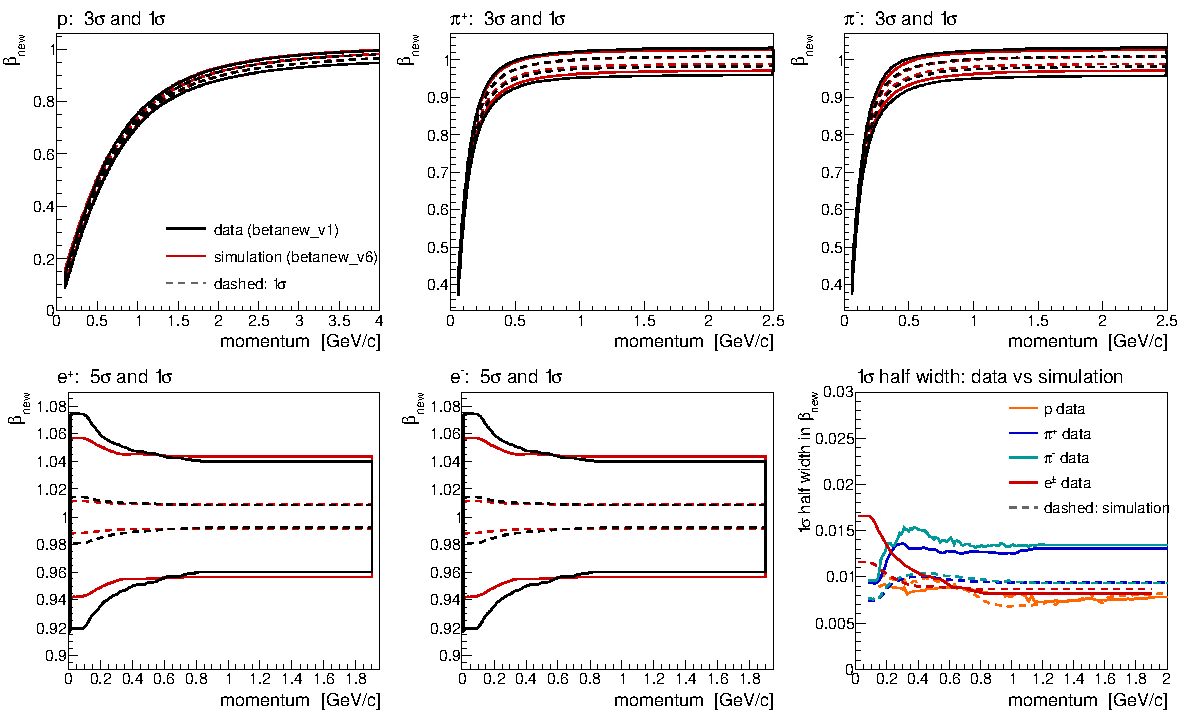
\includegraphics[width=\textwidth]{figs_exp/pid_polygons_v1_v6.pdf}
\caption{PID polygons of the data (\code{betanew_v1}, black) and of the simulation (\code{betanew_v6}, red)
against the momentum without energy-loss correction: solid, level used in PAT (p, $\pi^\pm$ $3\sigma$; $e^\pm$
$5\sigma$); dashed, $1\sigma$. Selection: none; the figure shows the cut contours themselves, no counts. Last panel: half width of the $1\sigma$ polygon, data solid, simulation dashed; the
data pion bands are 30--50\,\% wider. Polygons only; no counts, no normalisation.}
\label{fig:pid_polygons}
\end{figure}

\textbf{PID pictures of the data.} The polygons were fitted on two samples without PID cut, which are also
the only data samples without one: H, the June 2026 hadron production (hypotheses \pipi and pp, all entries
including isBest $=-1$, days 034, 045, 049, 062, first 40\,M entries per file, tracks without ring), and L, the
June 2026 lepton production (\ee hypothesis on days 036, 045, 050, 062; \ppee on all 29 days). The analysed
production (``betanew'') has the PID applied. Figures~\ref{fig:pid_hadrons}--\ref{fig:pid_all} show the
samples before the cut, Figs.~\ref{fig:pid_final} and~\ref{fig:pid_slots} the tracks of the analysed combinations;
Table~\ref{tab:pid_samples} gives the fractions inside the polygons. These fractions are \emph{not}
efficiencies: the samples contain all combinations including wrong hypotheses, and the reference track shifts
its partners (17\,\% of the \pim in \pipi and 13\,\% of the $e^-$ in \ppee have $\betanew>1.3$). PID
efficiencies must come from complete simulated combinations, as in Part~I.

\begin{figure}[!htbp]
\centering
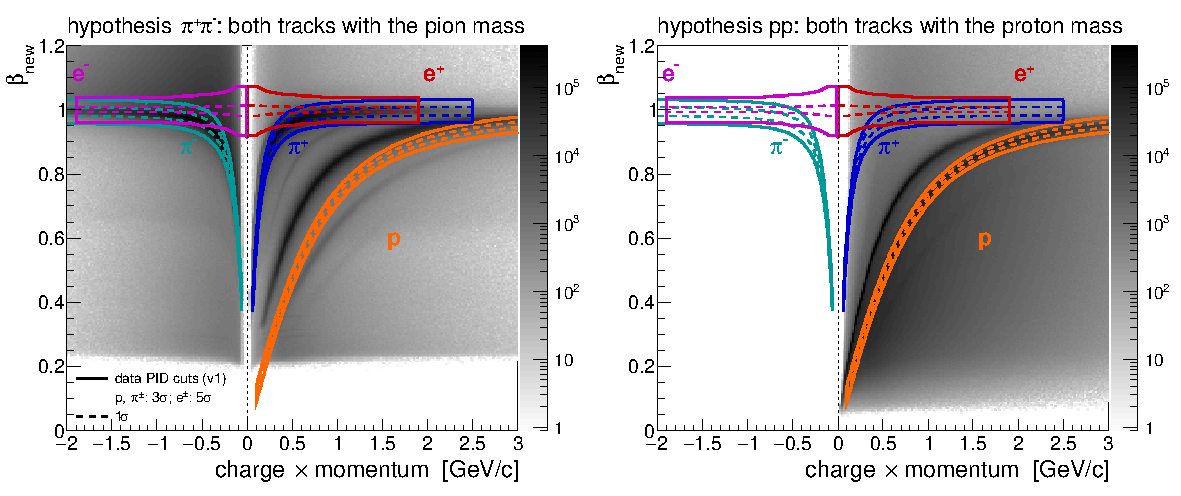
\includegraphics[width=\textwidth]{figs_exp/pid_banana_hadrons.pdf}
\caption{$\betanew$ against charge $\times$ momentum for tracks without a RICH ring before the PID cut. Selection: data without any PID cut (sample H): June 2026 hadron production, all entries of the hypothesis, i.e.\ all isBest values (also the combinations that fail the PID), days 034/045/049/062, first 40\,M entries per file, tracks without a RICH ring, a reconstructed event vertex ($\vz>-500$\,mm), no trigger condition, no other cut. Left: hypothesis \pipi (both tracks with the pion
mass); right: hypothesis pp (both with the proton mass). Lines: data polygons \code{betanew_v1} (p, $\pi^\pm$
$3\sigma$, $e^\pm$ $5\sigma$ solid; $1\sigma$ dashed); negative species at negative charge $\times$ momentum.
Protons in the pion hypothesis and pions in the proton hypothesis lie halfway between the bands,
Eq.~(\ref{eq:half}). Same colour scale in both panels; track entries, no normalisation.}
\label{fig:pid_hadrons}
\end{figure}

\begin{figure}[!htbp]
\centering
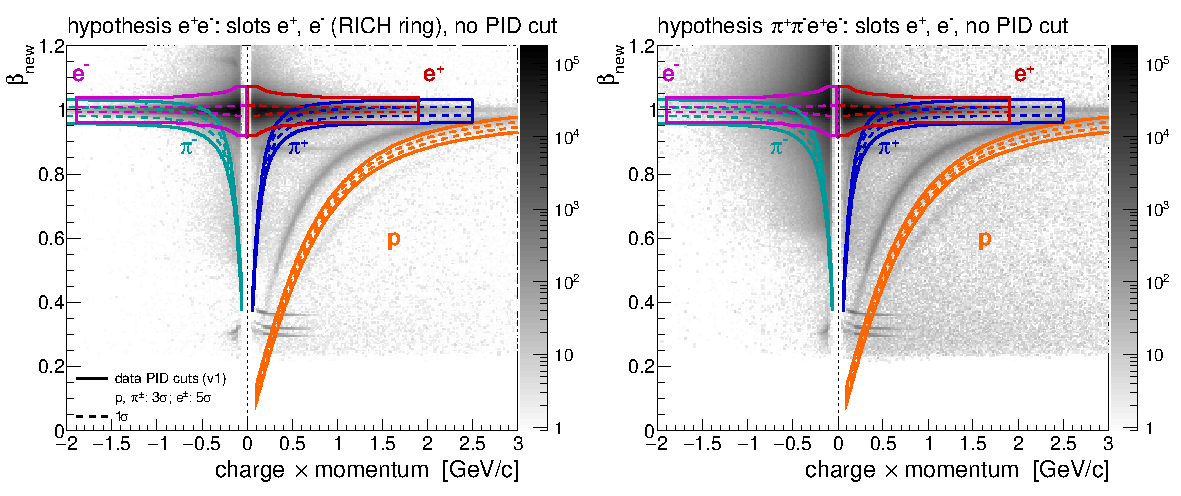
\includegraphics[width=\textwidth]{figs_exp/pid_banana_leptons.pdf}
\caption{Lepton candidates (tracks with a RICH ring) before the PID cut. Selection: data without any PID cut (sample L): June 2026 lepton production, all entries (all isBest values), tracks with a RICH ring, a reconstructed event vertex ($\vz>-500$\,mm), no trigger condition, no other cut. Left: \ee hypothesis, slots $e^+$ and $e^-$ (days
036, 045, 050, 062); right: lepton slots of the \ppee hypothesis (29 days). Lines as in
Fig.~\ref{fig:pid_hadrons}. The weak curved bands are hadrons with a random ring measured with the electron
mass; the horizontal structures at $\betanew=0.30$--0.37 and $p<0.6$\,\GeVc are not identified. Track entries,
no normalisation.}
\label{fig:pid_leptons}
\end{figure}

\begin{figure}[!htbp]
\centering
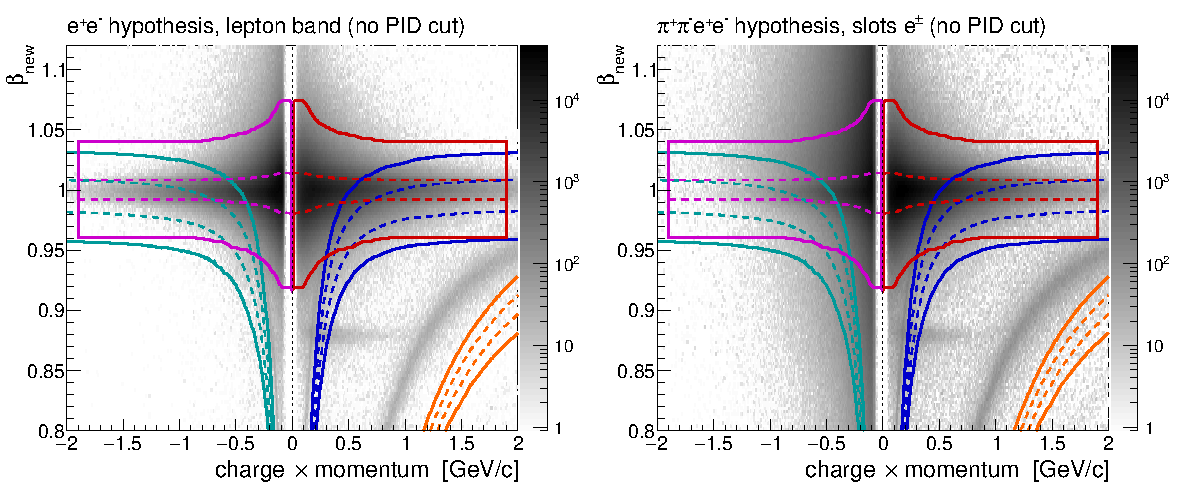
\includegraphics[width=\textwidth]{figs_exp/pid_banana_leptons_zoom.pdf}
\caption{The lepton band of Fig.~\ref{fig:pid_leptons} enlarged ($|$charge $\times$ momentum$|<2$\,\GeVc,
$\betanew=0.80$--1.12). Selection: the same as in Fig.~\ref{fig:pid_leptons} (sample L): data without any PID cut, June 2026 lepton production, all entries, tracks with a RICH ring, $\vz>-500$\,mm, no trigger condition; left the \ee hypothesis (days 036, 045, 050, 062), right the lepton slots of \ppee (29 days). Above about 0.4\,\GeVc the pion polygons overlap the $e^\pm$
polygons: there leptons and pions are separated by the RICH ring, not by $\betanew$.}
\label{fig:pid_leptons_zoom}
\end{figure}

\begin{figure}[!htbp]
\centering
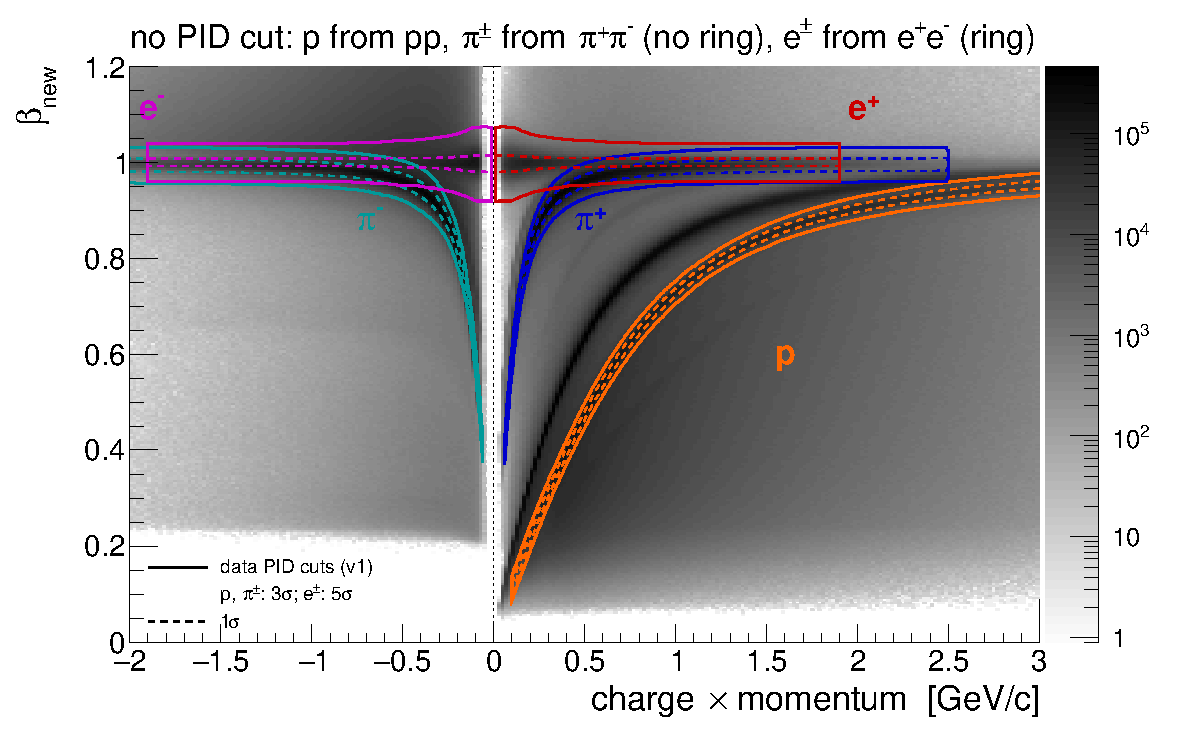
\includegraphics[width=\textwidth]{figs_exp/pid_banana_all.pdf}
\caption{All species, each in a slot of its own mass hypothesis, before the PID cut. Selection: data without any PID cut: p from the pp hypothesis and $\pi^\pm$ from the \pipi hypothesis (sample H: June 2026 hadron production, days 034, 045, 049, 062, first 40\,M entries per file, no ring), $e^\pm$ from the \ee hypothesis (sample L: June 2026 lepton production, days 036, 045, 050, 062, ring); $\vz>-500$\,mm, all entries (all isBest values), no trigger condition, no other cut. Lines: data polygons at the PAT level
(solid) and $1\sigma$ (dashed). The band between the \pip and the proton band holds protons measured with the
pion mass and pions measured with the proton mass. Track entries, no normalisation.}
\label{fig:pid_all}
\end{figure}

\begin{figure}[!htbp]
\centering
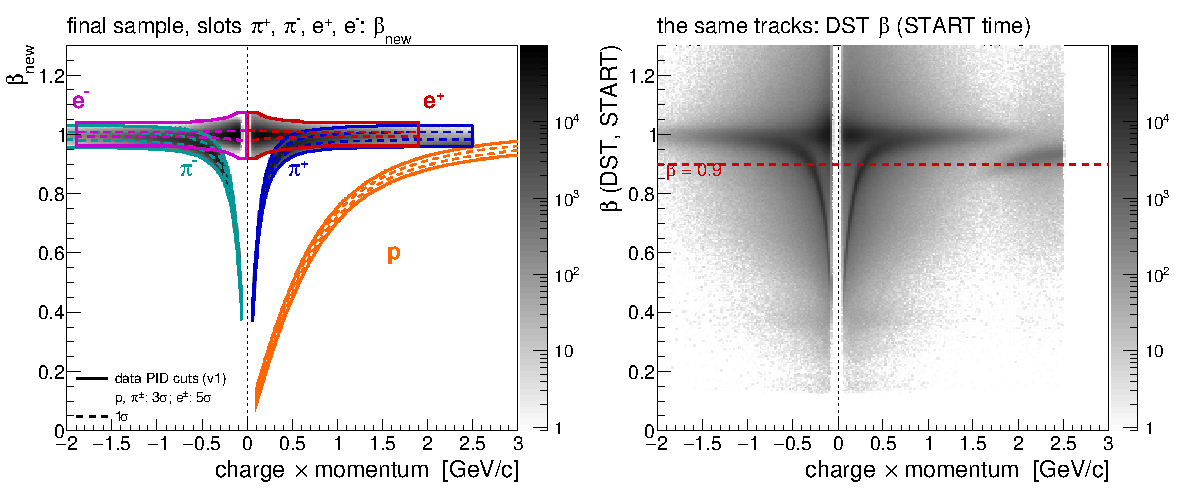
\includegraphics[width=\textwidth]{figs_exp/pid_banana_final.pdf}
\caption{Tracks of the analysed \ppee combinations (``betanew'' production; 4.78\,M combinations $\times$ 4 slots). Selection: data, the \ppee counts written by FAT, 29 days, after the \betanew identification of PAT (p, $\pi^\pm$ $3\sigma$, $e^\pm$ $5\sigma$; leptons with a RICH ring): all combinations (isBest $\ge0$), event vertex $\vz>-500$\,mm, \ptthreecap{}; no target-region cut, no momentum-correction requirement. Left: $\betanew$ with the data
polygons; right: the DST velocity of the same tracks measured against the START time, with the lepton-pass
limit $\beta=0.9$ of the track sorter (\S\ref{sec:sorter}). Track entries, no normalisation.}
\label{fig:pid_final}
\end{figure}

\begin{figure}[!htbp]
\centering
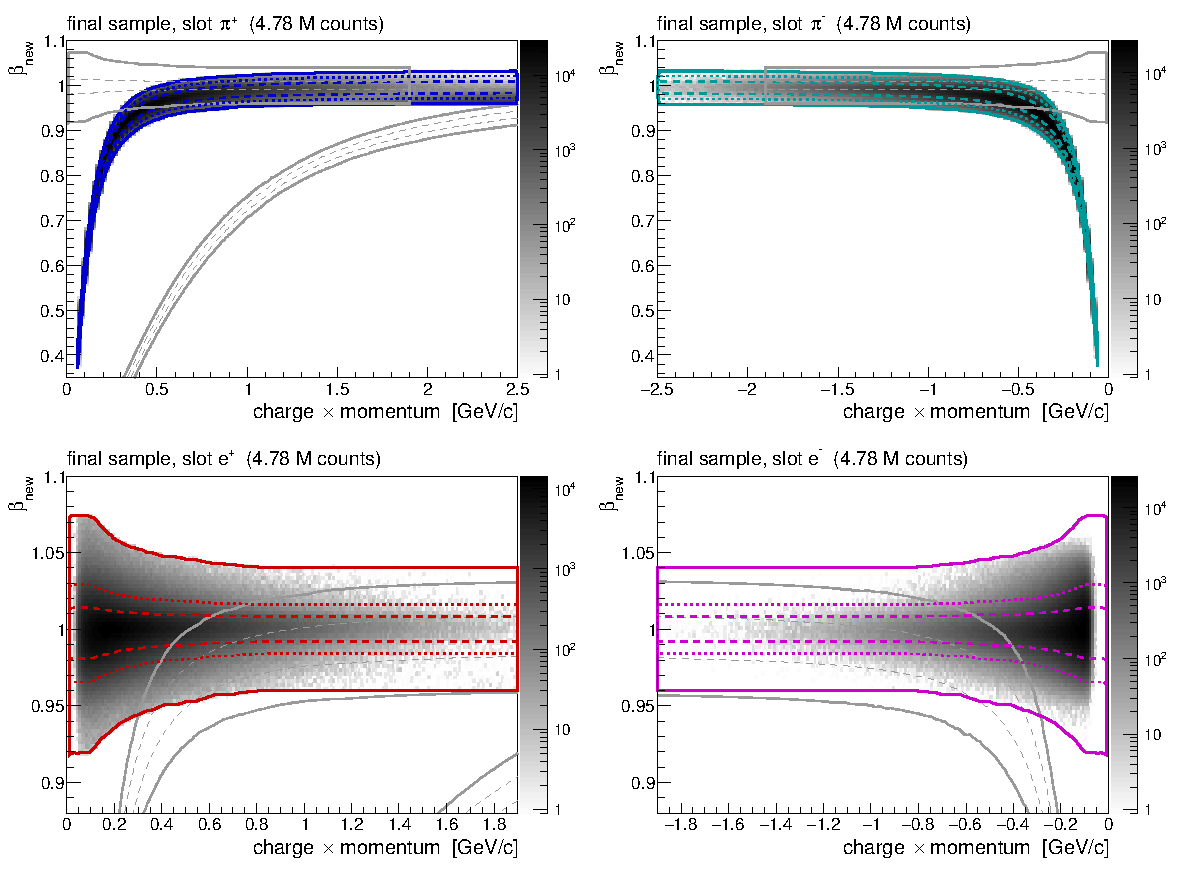
\includegraphics[width=\textwidth]{figs_exp/pid_banana_final_slots_cnt.pdf}
\caption{Analysed combinations per slot (\pip, \pim, $e^+$, $e^-$): $\betanew$ with
the slot's own polygon in colour (solid: PAT level, $3\sigma$ for $\pi$, $5\sigma$ for $e$; dashed $1\sigma$;
dotted $2\sigma$) and the other polygons in grey. Selection: as in Fig.~\ref{fig:pid_final}: data, the \ppee counts written by FAT, 29 days, after the \betanew identification of PAT (p, $\pi^\pm$ $3\sigma$, $e^\pm$ $5\sigma$; leptons with a RICH ring): all combinations (isBest $\ge0$), event vertex $\vz>-500$\,mm, \ptthreecap{}; no target-region cut, no momentum-correction requirement. All tracks lie inside the PAT polygon; 69--75\,\% inside
$1\sigma$. Above 1.9\,\GeVc most \pip-slot tracks (about 80\,\%) are protons; they pile up at the lower edge of
the \pip polygon ($\betanew=0.958$--0.975), which the logarithmic colour scale hides. They are 3\,\% of all
\pip-slot tracks (Table~\ref{tab:pid_pip_protons}). Track entries, no normalisation.}
\label{fig:pid_slots}
\end{figure}

\inputplaincode{tables_exp/pid_samples_cnt.tex}

\textbf{The analysed sample.} Every track of the 4\,783\,467 analysed combinations was tested exactly against the
polygons: 100.00\,\% of all four slots lie inside their PAT polygon (a check of the production). Inside
$1\sigma$ are 69.2\,\% (\pip), 72.1\,\% (\pim), 72.1\,\% ($e^+$) and 75.1\,\% ($e^-$), inside $2\sigma$ 90.9, 94.1,
92.5 and 95.2\,\%, and 98.13/99.33\,\% of the $e^+$/$e^-$ inside $3\sigma$. A Gaussian cut at the PAT level would give
68.5\,\% ($3\sigma$, pions) or 68.3\,\% ($5\sigma$, leptons) inside $1\sigma$ and 95.7/95.4\,\% inside $2\sigma$: the \pip and $e^+$
distributions have wider tails. 43.7\,\% of the \pip and 45.8\,\% of the
\pim lie also inside the $e$ polygon of the same charge, and 11.3\,\% of the $e^+$ and 5.0\,\% of the $e^-$ inside
the pion polygon: above about 0.4\,\GeVc the RICH ring, not $\betanew$, separates them. The selection ``pre''
gives the same picture.

\textbf{Protons in the \pip slot} (Table~\ref{tab:pid_pip_protons}). A proton measured with the pion mass has
$1/\betanew=(1/\beta_p+1/\beta_\pi)/2$, Eq.~(\ref{eq:half}); above about 2\,\GeVc this lies inside the \pip polygon.
The share was estimated per momentum bin from the DST velocity (share of \pip-slot tracks below the midpoint of
the pion and proton velocities, minus the same share of the \pim slot, divided by one minus the latter): 0.1\,\%
at 0.5--1.0\,\GeVc, 26.9\,\% at 1.5--1.9\,\GeVc, 78--82\,\% above 1.9\,\GeVc; 3.15\,\% of all \pip entries (3.24\,\%
with a cut on the DST mass, a method difference of 3\,\% relative). In the analysis windows they are negligible:
0.15\,\% (peak nominal, peak window) and 0.06\,\% (bump nominal, bump window). A cut $p(\pip)<1.5$\,\GeVc would
remove them if wanted.

% pid_pip_protons_cnt.tex: copy of pid_pip_protons.tex with "rows" -> "counts" (analyst, 15 Nov 2026; Part II writer, integ4)
% generated by plots/exp_report/pid_draw.C
\begin{table}[H]
\centering
\caption{Protons in the $\pi^+$ slot of the analysed combinations (isBest $\geq 0$, $z>-500$\,mm, PT3), estimated from the START-based DST velocity: share of $\pi^+$-slot tracks with $\beta_{\mathrm{DST}}$ below the midpoint of the pion and proton velocities, minus the same share for the $\pi^-$ slot (no antiprotons), divided by one minus the $\pi^-$ share. Momentum $p$ without energy-loss correction.}
\label{tab:pid_pip_protons}
\footnotesize
\begin{tabular}{@{}l r r r r r@{}}
\toprule
$p$ [GeV/$c$] & $\pi^+$ tracks & share of slot & $f(\pi^+)$ & $f(\pi^-)$ & protons [\%] \\
\midrule
0.5--1.0 & 1415918 & 0.2960 & 0.054 & 0.053 & 0.1 \\
1.0--1.5 & 260237 & 0.0544 & 0.101 & 0.095 & 0.7 \\
1.5--1.9 & 53854 & 0.0113 & 0.366 & 0.134 & 26.9 \\
1.9--2.2 & 67362 & 0.0141 & 0.815 & 0.176 & 77.6 \\
2.2--2.5 & 100054 & 0.0209 & 0.862 & 0.252 & 81.6 \\
\midrule
all & 4783467 & & & & 3.15 \\
\bottomrule
\end{tabular}
\end{table}


\subsection{Selection}
\label{sec:sel}
The base selection ``pre'' is
\begin{enumerate}
\setlength{\itemsep}{0pt}
\item all combinations that passed the PID, isBest $\ge0$;
\item event vertex $\vz>-500$\,mm and PT3, \code{trigbit} $==8192$ (both applied by FAT);
\item corrected momenta for all four particles, \code{cor_ok} $=1$ (\S\ref{sec:corok});
\item target region $\vz>-160$\,mm (adopted analysis cut; \S\ref{sec:vertex}).
\end{enumerate}
It is identical to the frozen BUMP selection of the simulation study. The cut variables are listed in
Table~\ref{tab:cuts}, the named selections of the data study in Table~\ref{tab:named}, the selections frozen in
the simulation study in Table~\ref{tab:frozen}, and the mass windows in Table~\ref{tab:windows}. All cuts act
in the same way on the unlike-sign and the like-sign counts.

\begin{table}[H]
\centering
\caption{Cut variables (notation: Table~\ref{tab:notation}). All are computed from the corrected momenta with
$T_{\mathrm{beam}}=4530$\,MeV and stored per entry in \code{scan_nt}; the pion-vertex flags and \dzpi are per-track quantities and
apply to like-sign counts in the same way.}
\label{tab:cuts}
\small
\begin{tabularx}{\textwidth}{@{}>{\raggedright\arraybackslash}p{3.2cm} L >{\raggedright\arraybackslash}p{3.3cm}@{}}
\toprule
Variable (code) & Meaning & Values used \\
\midrule
OA (\code{oa}) & opening angle of the \ee pair (lab) & $>2^\circ$ (variant only) \\
\alab (\code{oa_lab}) & angle between the \pipi and the \ee momenta (lab) & $<55^\circ$, $<40^\circ$ \\
\Mpipi (\code{mpipi}) & invariant mass of the pions & $>0.30$, $<0.41$\,\GeVcc \\
\aeta ($\eta$-rest angle) & angle between \pipi and \ee in the rest frame of a hypothetical $\eta$ (measured \ppee
  momentum, mass $m_\eta$); a band-pass in \Mfour & $>140^\circ$ (old selections) \\
\MMfour (\code{mm4}) & missing mass of \ppee: mass of (beam + target $-$ \ppee) & $<2.85$\,\GeVcc (PEAK) \\
$p_{T,4}$, $y_4$ & transverse momentum (lab), c.m.\ rapidity of \ppee & shown only \\
\vz & event-vertex $z$ & $>-500$ (FAT), $>-160$\,mm \\
vertex & both pions used in the event-vertex fit (\code{pip_isUsedVertex}, \code{pim_isUsedVertex}) & flag \\
\dzpi (\code{dz_pi}) & Eq.~(\ref{eq:dzpi}) & $<40$\,mm (PEAK, DIRECT) \\
\Mee (\code{mee}) & mass of the lepton pair & 15.5--24.5\,\MeVcc (X17) \\
\bottomrule
\end{tabularx}
\end{table}

\begin{table}[H]
\centering
\caption{Named selections of the data study (all include ``pre''; notation: Table~\ref{tab:notation}). ``peak
nominal'' and ``bump nominal'' were chosen on these data in the first cut-scan study (2026-11-11); ``slides'' and
``old code'' are earlier selections (``old code'' $=$ the FAT flag \code{sel_pass_cor}).}
\label{tab:named}
\small
\begin{tabularx}{\textwidth}{@{}>{\raggedright\arraybackslash}p{4.0cm} L@{}}
\toprule
Name & Cuts in addition to ``pre'' \\
\midrule
pre + vertex & both pions in the event-vertex fit \\
peak nominal & $\alab<55^\circ$, $\Mpipi>0.30$\,\GeVcc \\
peak nominal + vertex & peak nominal + both pions in the vertex fit \\
bump nominal & $\alab<40^\circ$, $0.30<\Mpipi<0.41$\,\GeVcc \\
bump nominal + vertex & bump nominal + both pions in the vertex fit \\
slides & $\alab<50^\circ$, $\Mpipi<0.46$\,\GeVcc, $\aeta>140^\circ$, OA$>2^\circ$ \\
old code & $\alab<50^\circ$, $\Mpipi<0.42$\,\GeVcc, $\aeta>140^\circ$ \\
\bottomrule
\end{tabularx}
\end{table}

\begin{table}[H]
\centering
\caption{Selections frozen in the simulation study (Part~I, Sect.~5.5--5.6), on top of ``pre''. They were
chosen on simulation truth alone, each as the loosest cell within $0.95\,F_{\mathrm{I,best}}$ of an exhaustive grid
(Part~I's $F_{\mathrm{I}}=S/\sqrt{S+B}$ on simulation, not the $F$ of this part),
with the freeze rule declared before the search. $\varepsilon$: simulated efficiency relative to ``pre''.
Notation: Table~\ref{tab:notation}.}
\label{tab:frozen}
\small
\begin{tabularx}{\textwidth}{@{}>{\raggedright\arraybackslash}p{1.6cm} >{\raggedright\arraybackslash}p{4.4cm} L@{}}
\toprule
Name & Simulation target & Cuts in addition to ``pre'' \\
\midrule
PEAK & $\eta\to\ppee$ and $\eta\to\pipi\gamma$ (conversion) in 0.5333--0.5587 & $\dzpi<40$\,mm, $\MMfour<2.85$\,\GeVcc ($\varepsilon=0.9310\pm0.0072$) \\
DIRECT & $\eta\to\ppee$ in the same window & $\dzpi<40$\,mm ($\varepsilon=0.9625\pm0.0005$) \\
BUMP & $\eta\to\pipi\piz$ in 0.4576--0.5255 & none: BUMP $=$ ``pre'' ($\varepsilon=1$) \\
X17 & $\eta\to\pipi X17$ & $0.5333\le\Mfour<0.5587$, $15.5\le\Mee<24.5$\,\MeVcc, both pions in the vertex fit \\
\bottomrule
\end{tabularx}
\end{table}

\begin{table}[H]
\centering
\caption{Mass windows in \Mfour [\GeVcc]. The data windows are used for every data-only number; the frozen
windows of the simulation study are centred on the simulated peak (0.5460, 2.1\,\MeVcc above the data peak) and
are used only where it is said.}
\label{tab:windows}
\small
\begin{tabularx}{\textwidth}{@{}l l L@{}}
\toprule
Region & Range & Origin \\
\midrule
data peak window & 0.53364--0.55416 & $0.5439\pm1.9\times5.4$\,\MeVcc (0.9426 of the Gaussian) \\
data bump window & 0.4550--0.5225 & first study; upper end $=$ lower bound of the peak fit \\
side bands & 0.5225--0.53364, 0.55416--0.56530 & side-band method (\S\ref{sec:proc}) \\
\Pmain fit range & 0.5225--0.6100 & frozen; lower bound where $\chi^2$ stops falling \\
sim.\ peak / bump window & 0.5333--0.5587 / 0.4576--0.5255 & frozen selections, Part~I \\
X17 \Mfour window, moved to the data scale & 0.5312--0.5566 & sim.\ window $\times\,0.5439/0.5460$ (Table~\ref{tab:x17win}) \\
\bottomrule
\end{tabularx}
\end{table}

\subsection{Measurement procedures}
\label{sec:proc}
The same procedures (implemented in \code{plots/ScanEngine.h}) are used in every chapter.

\textbf{Spectra and CB.} \Mfour is histogrammed in 2.5\,\MeVcc bins for the three hypotheses in one pass over
the entries. The CB is $2\sqrt{N_{++}N_{--}}$ in 10\,\MeVcc bins, linearly interpolated to the 2.5\,\MeVcc bins,
Eq.~(\ref{eq:cb}); the signal estimate is $N-\mathrm{CB}$.

\textbf{$\eta$ peak, \Pmain.} A $\chi^2$ fit of $N-\mathrm{CB}$ in 0.5225--0.6100\,\GeVcc with
\begin{equation}
N_i-\mathrm{CB}_i = S\,G(m_i;\,\mu=0.5439\,\mathrm{GeV}/c^2,\ \sigma=5.4\,\mathrm{MeV}/c^2)\,\Delta m + p_0+p_1m_i+p_2m_i^2 ,
\label{eq:pmain}
\end{equation}
with the Gaussian frozen (position and width from the free fit on $\alab<50^\circ$ without $\vz$ cut:
$0.54388\pm0.00049$\,\GeVcc, $5.44\pm0.60$\,\MeVcc). The covariance contains the expected Poisson variance
(iterated) and the covariance of the interpolated CB. $S$ is the content of the whole Gaussian, ``stat'' its fit
error. \textbf{Model spread (old envelope, chapter tables and figures)}: the fit is repeated with polynomial
order 1--4, four ranges (0.520--0.590, 0.515--0.610, 0.510--0.620, 0.505--0.650) and the width $\pm0.5$\,\MeVcc
(48 variations); the spread is half of (max $-$ min) of $S$ over the variations with $p>0.05$. It is
19.9--24.6\,\% of $S$ for the six candidate selections (26.5\,\% without the $\vz$ cut, 30\,\% for the X17 band).
Three of its four ranges start below the highest bump edge (0.5202), and a half range over many variations also
collects their statistical noise. \textbf{Model uncertainty (revised, quoted in the summaries)}: the rms of $S$ over
an edge-safe grid of 144 variations with every lower bound $\ge0.5225$, 9--11\,\% of $S$ (\S\ref{sec:fixmodel},
Table~\ref{tab:fix_spread}). $B$ is pol2 + CB in the data peak window and $S/B$ uses the $S$ in the window.
$F=S/\mathrm{stat}$ compares selections on the same data; it is not a significance.
$F_{\mathrm{tot}}=S/\sqrt{\mathrm{stat}^2+\mathrm{model}^2}$ (with the old envelope in the chapter tables, with the
revised model uncertainty in \S\ref{sec:fixmodel}).
\textbf{Controls}: a Poisson-likelihood fit of the unsubtracted $N$ with the CB as fixed background
($P_{\mathrm{pois}}$); the same frozen fit on $N_{++}$ and $N_{--}$ (null tests, \S\ref{sec:cbnull}); fits at
displaced positions. The lower fit bound matters: $S=4114$, 4205, 4319, 4359 for 0.515, 0.520, 0.5225, 0.525
(pol2; first study, $\alab<50^\circ$, no $\vz$ cut); with higher polynomial orders the lower bounds below 0.5225
give larger $S$ (Fig.~\ref{fig:fix_spread}).

\textbf{Bump, edge step $E$.} The bump has no peak; its visible sign is the kinematic edge of
$\eta\to\pipi\piz$, $\piz\to\ee\gamma$ with the photon lost. For a given \Mpipi and $\Mee\to0$ (true masses),
\begin{equation}
M_4^{\max}(\Mpipi)^2=m_\eta^2-m_\eta\,(E^*-p^*),\qquad E^*=\frac{m_\eta^2+m_{\pi^0}^2-M_{\pi\pi}^2}{2m_\eta},\qquad
p^*=\sqrt{E^{*2}-m_{\pi^0}^2},
\label{eq:m4max}
\end{equation}
the photon taking its smallest possible energy. A pair with $\Mee>0$ leaves less energy to the photon, so its
limit is higher: at $\Mpipi=2m_\pi$ it rises from 0.520 ($\Mee\to0$) to about 0.524 and 0.533\,\GeVcc (measured scale)
for $\Mee=50$ and 100\,\MeVcc. $M_4^{\max}$ is therefore the edge of the dominant small-\Mee part of the bump, not a
hard limit for every count. In four \Mpipi slices (0.30--0.34, 0.34--0.37, 0.37--0.39, 0.39--0.40\,\GeVcc)
$N-\mathrm{CB}$ is fitted with
\begin{equation}
N-\mathrm{CB} = \mathrm{pol2}\,[+\,\eta\ \text{Gaussian}] + h\;\tfrac12\,\mathrm{erfc}\!\left(\frac{m-m_{\mathrm{edge}}}{\sqrt2\cdot5.4\,\mathrm{MeV}/c^2}\right),
\qquad E=\sum_{4\ \text{slices}} h ,
\label{eq:edge}
\end{equation}
with the edge \emph{fixed} on the measured scale, $m_{\mathrm{edge}}=0.9927\,M_4^{\max}(\Mpipi/0.9970)$ (\Mfour scale
0.9927 of the $\eta$ peak, \Mpipi scale 0.9970 from K$^0_S$), and the step averaged over 21 values of \Mpipi
across the slice. $h$ is the height of the drop in counts per 2.5\,\MeVcc; $E$
measures how visible the edge is and is \emph{not} a yield. Model spread: polynomial order 2/3, half range
35/45/55\,\MeVcc, smearing 4.4/5.4/6.4\,\MeVcc (18 variations with $p>0.05$, added linearly over the slices). The
statistical error of $E$ is the fit error; a bootstrap with 200 replicas of the data (Part~III) confirms it (0.98--1.04 of the fit
error), while the earlier calibration with 40 halvings had suggested a factor 1.2, which is not confirmed (\S\ref{sec:fixmodel}). The slice 0.40--0.41 is fitted (Table~\ref{tab:res_bump}) but neither drawn nor
used in $E$; the control slice 0.42--0.46 lies above the kinematic limit
$m_\eta-m_{\pi^0}=0.413$\,\GeVcc (edge set at 0.5150\,\GeVcc), where no step is expected. $W$ is $N-\mathrm{CB}$ in
the bump window (bump and physical background), $N_b$ the counts there, $Q=E/\sqrt{N_b}$.

\textbf{ECAL-tagged $\eta$, $T$ (verification only).} Counts with an ECAL photon of good quality (\code{ecal_pid},
$0.8<\beta<1.2$, energy $>100$\,MeV) and $0.119\le M(\ee\gamma)<0.173$\,\GeVcc, $\Mee<0.10$\,\GeVcc;
$m_{5c}=M(\ppee\gamma)$ with the photon energy rescaled so that $M(\ee\gamma)=m_{\pi^0}$. $T$ is the content of a
frozen Gaussian (0.5463\,\GeVcc, 6.2\,\MeVcc) + pol2 fit of $N-\mathrm{CB}$ in $m_{5c}=0.49$--0.62\,\GeVcc. It measures
the same decay as the bump, with the photon found.

\textbf{Efficiencies and gains.} $\varepsilon_S=S_{\mathrm{pass}}/(S_{\mathrm{pass}}+S_{\mathrm{fail}})$ from
\Pmain fits of the counts that pass and that fail a cut (stat.\ error from the two fits, their small correlation
neglected; model error from the variations in which both fits have $p>0.05$); $\varepsilon_B$ is the kept share
of pol2 + CB in the peak window. A cut improves the statistical precision of the peak only if
$\varepsilon_S>\sqrt{\varepsilon_B}$. For the bump, $\mathrm{gain}=(\text{kept share of }E\text{ or }T)/\sqrt{\text{kept share of }N_b}$;
a gain above 1 makes the bump more visible.

\textbf{Side-band method} (content of the peak in classes of \Mee or OA, and the X17 band). With the peak-window
region $R_{\mathrm{pk}}$ (data peak window) and the side-band region $R_{\mathrm{SB}}$,
\begin{equation}
D=(N-\mathrm{CB})_{R_{\mathrm{pk}}}-r_{SB}\,(N-\mathrm{CB})_{R_{\mathrm{SB}}},\qquad S_{\mathrm{SB}}=\frac{D}{f_{\mathrm{pk}}-r_{SB}\,f_{SB}},
\label{eq:sb}
\end{equation}
where $r_{SB}$ is the ratio of the integrals of the \Pmain pol2 of the whole selection over $R_{\mathrm{pk}}$ and over $R_{\mathrm{SB}}$
(0.9163 for ``pre''), and $f_{\mathrm{pk}}=0.9426$, $f_{SB}=0.0574$ are the shares of the frozen Gaussian in $R_{\mathrm{pk}}$ and $R_{\mathrm{SB}}$
(this removes the peak tails in the side bands). The CB of each class comes from the like-sign counts of the same
class; the errors use the event groups with the weights $+1$ and $-r_{SB}$; the model error takes $r_{SB}$ from
pol1 and pol3.

\textbf{Sculpting test and optimisation bias}: \S\ref{sec:sculpt} and \S\ref{sec:bias}.

\subsection{Software chain}
\label{sec:chain}
\begin{enumerate}
\setlength{\itemsep}{0pt}
\item \textbf{PAT} (\code{pat3}, tag \code{prod-feb22-betanew-2026-10-28}): DST $\to$ hypothesis trees with PID on
      $\betanew$ and ranking.
\item \textbf{FAT} (this repository, branch \code{pp45_pippimepem}, commit \code{38d168f}): $\vz>-500$\,mm, PT3,
      kinematics with $T_{\mathrm{beam}}=4530$\,MeV, flags, ntuple \code{scan_nt}; run with \code{run_parallel.sh}.
\item \textbf{Compact file} (\code{plots/scan_prepare.C}): \code{scan_v2/scan_compact.root}, trees \code{us},
      \code{pp}, \code{mm}, with event groups, folds and the pion-vertex variables.
\item \textbf{Engine} \code{plots/ScanEngine.h}: \code{Load}, selections, \code{FillMany} (all spectra in one
      pass, event-group variances), \code{FitPeakMain}, \code{PeakModelSpread}, \code{FitEdgeStep}, CB.
\item \textbf{Report macros} \code{plots/exp_report/<prefix>_*.C} (prefixes \code{prep}, \code{smp}, \code{pid},
      \code{spec}, \code{cb}, \code{opt}, \code{res}), each with an independent verification macro
      \code{verify_<prefix>_*.C}; figures in \code{docs/latex/figs_exp/}, tables in
      \code{docs/latex/tables_exp/} (Appendix~\ref{app:files}).
\end{enumerate}

%======================================================================
\section{Spectra and combinatorial background}
\label{sec:spec}
%======================================================================

\inshort{The CB is a small part of the background (CB$/N=0.072$ for PEAK in the peak window); the like-sign spectra show no $\eta$ peak and no bump edge in \Mfour (in the distance to the edge, $u$, the $e^-e^-$ counts show a step, 4.7$\sigma$, from lepton pairs of the two \piz photons, which the CB subtracts as designed); $S$ and $E$ change by at most 0.1\,\% for CB$\pm3$\,\% and by at most 1\,\% and 3\,\% for a 38--45\,\% larger CB. The absolute CB normalisation cannot be checked with data alone; $k=1$ is kept.}

\subsection{\texorpdfstring{The spectrum of $M(\pi^+\pi^-e^+e^-)$}{The M4 spectrum}}
\label{sec:m4}
Figure~\ref{fig:m4_overview} shows \Mfour of six selections with the CB and $N-\mathrm{CB}$, Fig.~\ref{fig:m4_zoom}
the region of the two signals. The spectrum is dominated by counts with a true \ee pair from one source and
pions from the same collision (the ``physical'' background, which the CB does not remove); the CB is only
5--11\,\% of the counts in the windows (CB$/N=0.052$--0.110 in Table~\ref{tab:spec_counts_pre}; 0.103 in the peak window of ``pre''), so $N$ and $N-\mathrm{CB}$ nearly overlap on a log
scale. The $\eta$ peak sits on a steeply rising spectrum; the bump is a shoulder ending at the kinematic edge
below the peak. Table~\ref{tab:spec_counts_pre} gives the counts of ``pre'' in the standard regions (with
OA$>2^\circ$ and isBest $=1$), Tables~\ref{tab:spec_counts_sel} and~\ref{tab:spec_counts_sel_oa2} $N-\mathrm{CB}$ of all
selections without and with OA$>2^\circ$, and Table~\ref{tab:spec_yields} the same as visible yields per
luminosity. The regions add up to the total exactly; a $\pm3$\,\% change of the CB moves the window counts by
$\Delta_{3\%}$ (238 counts in the peak window of ``pre'').

Two remarks on the frozen selections. (i) Above $\Mfour=0.62$\,\GeVcc PEAK and DIRECT are identical, because
$\MMfour\le\sqrt{s}-\Mfour<2.85$\,\GeVcc for $\Mfour>0.62$\,\GeVcc ($\sqrt{s}=3.467$\,GeV): the cut $\MMfour<2.85$ acts only at low \Mfour; in
the peak and bump windows it removes 10.3\,\% of $N-\mathrm{CB}$ of ``pre''. (ii) The like-sign composition differs:
$N_{--}/N_{++}$ in the peak window is about 6.7 for peak nominal + vertex and 4.1 for PEAK
(\MMfour removes $e^-e^-$ counts more strongly).

\begin{figure}[H]
\centering
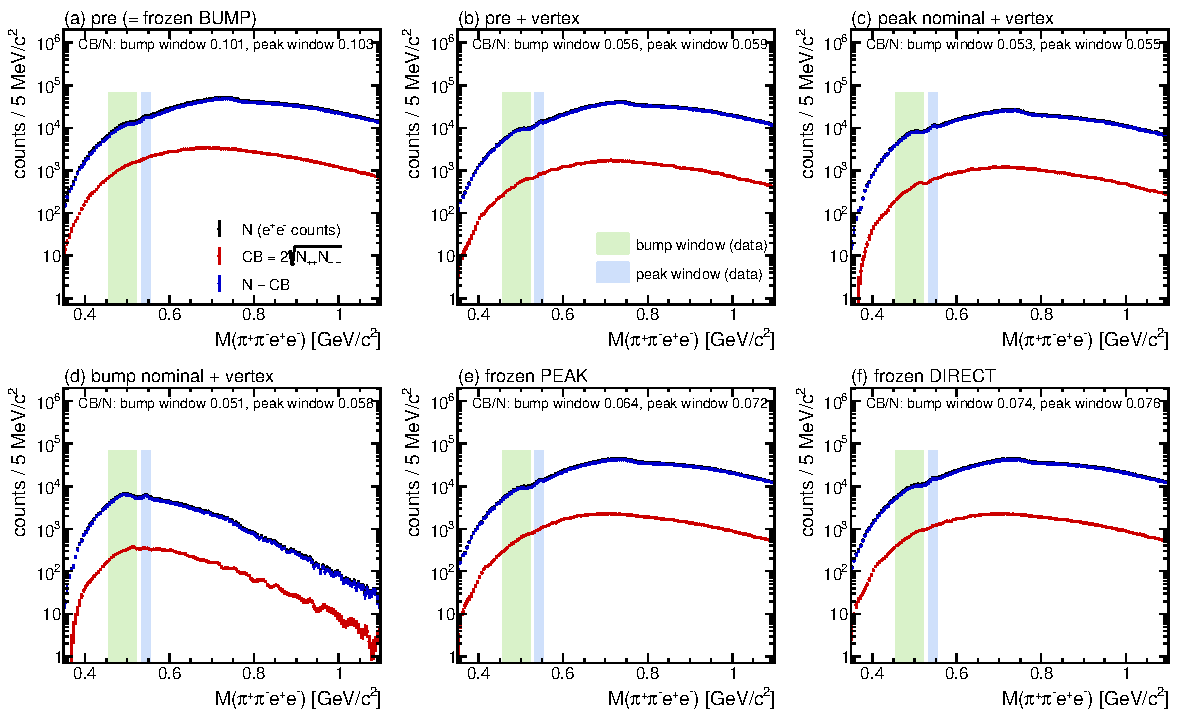
\includegraphics[width=\textwidth]{figs_exp/spec_m4_overview_cnt.pdf}
\caption{\Mfour of the data ($T_{\mathrm{beam}}=4.53$\,GeV, PT3, $\vz>-500$\,mm, corrected momenta), all stored combinations
(isBest $\ge0$), 5\,\MeVcc bins, log scale. Selection: data; every panel has the base cuts: \ptthreecap{}, event vertex in the target region ($\vz>-160$\,mm), particles identified by their START-free velocity \betanew (pions within $3\sigma$, leptons within $5\sigma$ of their band; leptons with a RICH ring, pions without), energy-loss-corrected momenta of all four tracks (\code{cor_ok} $=1$), all stored \ppee combinations of each event (isBest $\ge0$) (``pre''). (a) ``pre'' only ($=$ BUMP); (b) + both pions used in the event-vertex fit (pre + vertex); (c) + the angle between the \pipi and \ee momenta in the laboratory below $55^\circ$ ($\alab<55^\circ$), $\Mpipi>0.30$\,\GeVcc and both pions in the vertex fit (peak nominal + vertex); (d) + $\alab<40^\circ$, $0.30<\Mpipi<0.41$\,\GeVcc and both pions in the vertex fit (bump nominal + vertex); (e) + both pion tracks within 40\,mm of the event vertex along the beam ($\dzpi<40$\,mm) and a missing mass of \ppee below 2.85\,\GeVcc ($\MMfour<2.85$\,\GeVcc; PEAK); (f) + $\dzpi<40$\,mm (DIRECT). Data windows: bump 0.4550--0.5225, peak 0.53364--0.55416\,\GeVcc. Black: unlike-sign counts $N$; red: CB $=2\sqrt{N_{++}N_{--}}$ (10\,\MeVcc
bins interpolated, $k=1$); blue: $N-\mathrm{CB}$ ($N$ is mostly hidden under it). Green and blue bands: data
bump and peak windows; the CB share in both is printed. Equal y ranges. Counts, not normalised to luminosity.}
\label{fig:m4_overview}
\end{figure}

\begin{figure}[H]
\centering
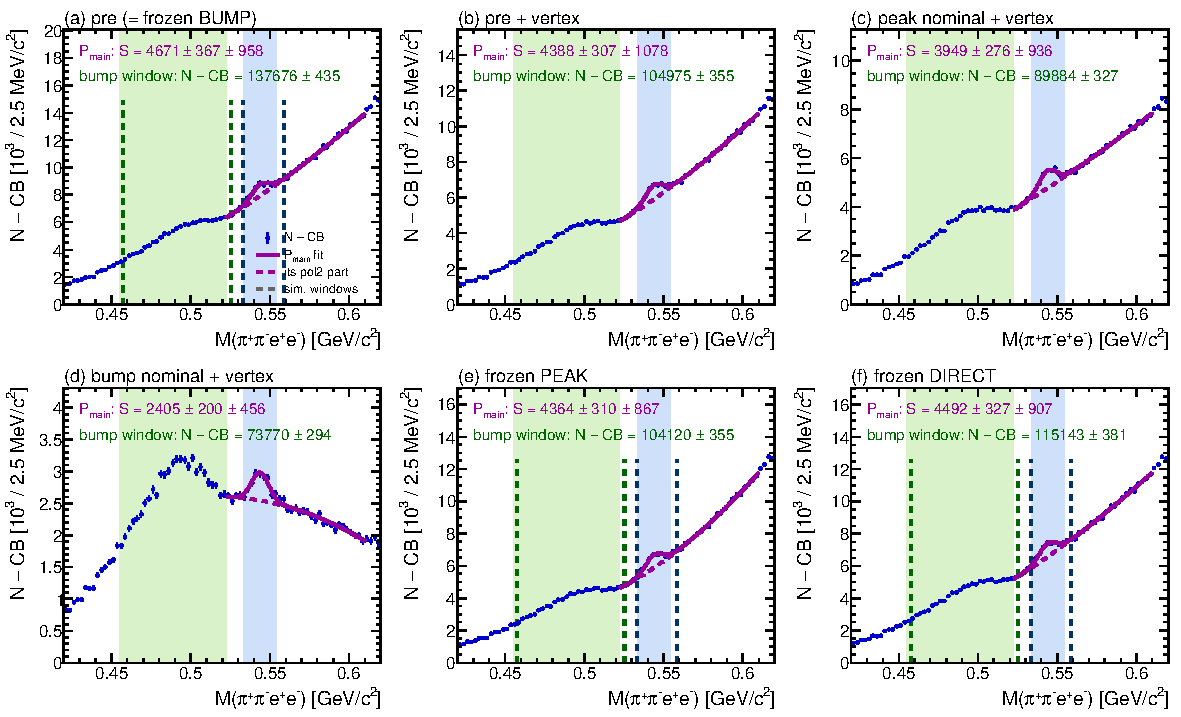
\includegraphics[width=\textwidth]{figs_exp/spec_m4_zoom.pdf}
\caption{$N-\mathrm{CB}$ of the six selections of Fig.~\ref{fig:m4_overview} in 0.42--0.62\,\GeVcc (2.5\,\MeVcc bins,
linear scale, $10^3$ counts; the y ranges differ), isBest $\ge0$, CB with $k=1$. Selection: data; every panel has the base cuts: \ptthreecap{}, event vertex in the target region ($\vz>-160$\,mm), particles identified by their START-free velocity \betanew (pions within $3\sigma$, leptons within $5\sigma$ of their band; leptons with a RICH ring, pions without), energy-loss-corrected momenta of all four tracks (\code{cor_ok} $=1$), all stored \ppee combinations of each event (isBest $\ge0$) (``pre''). (a) ``pre'' only ($=$ BUMP); (b) + both pions used in the event-vertex fit (pre + vertex); (c) + the angle between the \pipi and \ee momenta in the laboratory below $55^\circ$ ($\alab<55^\circ$), $\Mpipi>0.30$\,\GeVcc and both pions in the vertex fit (peak nominal + vertex); (d) + $\alab<40^\circ$, $0.30<\Mpipi<0.41$\,\GeVcc and both pions in the vertex fit (bump nominal + vertex); (e) + both pion tracks within 40\,mm of the event vertex along the beam ($\dzpi<40$\,mm) and a missing mass of \ppee below 2.85\,\GeVcc ($\MMfour<2.85$\,\GeVcc; PEAK); (f) + $\dzpi<40$\,mm (DIRECT). Data windows: bump 0.4550--0.5225, peak 0.53364--0.55416\,\GeVcc. Simulation-centred windows (dashed, (a), (e), (f)): peak 0.5333--0.5587, bump 0.4576--0.5255\,\GeVcc. Bands: data bump and peak windows;
dashed lines (a, e, f): the simulation-centred windows of the frozen selections. Magenta: reference \Pmain fit
(frozen Gaussian 0.5439\,\GeVcc, 5.4\,\MeVcc, + pol2 in 0.5225--0.6100); dashed: its polynomial. Printed: $S\pm$stat$\pm$model
spread and $N-\mathrm{CB}$ in the bump window. Counts, not normalised to luminosity.}
\label{fig:m4_zoom}
\end{figure}

% spec_counts_pre_cnt.tex: copy of spec_counts_pre.tex with "rows" -> "counts" (analyst, 15 Nov 2026; Part II writer, integ4)
% written by plots/exp_report/spec_m4.C -- selection pre, counts in the standard M4 regions
\begin{table}[H]
\centering
\scriptsize
\caption{Counts of the selection \emph{pre} (corrected momenta, $\mathrm{cor\_ok}=1$, event vertex $z>-160$~mm, PT3, all stored combinations $\mathrm{isBest}\ge0$) in the standard regions of $M(\pi^+\pi^-e^+e^-)$. $N$: unlike-sign counts; CB $=2\sqrt{N_{++}N_{--}}$ (10~MeV/$c^2$ bins interpolated, $k=1$). Errors: statistical, with the event-group correlation. $\Delta_{3\%}$: change of $N-\mathrm{CB}$ for a 3~\% change of CB. $Y=(N-\mathrm{CB})\times\frac{64}{63}/L$ with $L=6079.2$~nb$^{-1}$ (counts per nb$^{-1}$; statistical error only; $L$ has a 6.9~\% uncertainty). Last two columns: $N-\mathrm{CB}$ with $\mathrm{OA}(e^+e^-)>2^\circ$ and with $\mathrm{isBest}=1$. Not corrected for acceptance or efficiency.}
\label{tab:spec_counts_pre}
\resizebox{\textwidth}{!}{\begin{tabular}{lrrrrrrrr}
\toprule
region [GeV/$c^2$] & $N$ & CB & CB/$N$ & $N-\mathrm{CB}$ & $\Delta_{3\%}$ & $Y$ [nb] & OA$>2^\circ$: $N-\mathrm{CB}$ & isBest$=1$: $N-\mathrm{CB}$ \\
\midrule
$<0.455$ & $50593\pm233$ & $4995\pm89$ & 0.099 & $45598\pm249$ & 150 & $7.62\pm0.04$ & $35348\pm226$ & $36193\pm214$ \\
bump window 0.455--0.5225 & $153183\pm406$ & $15507\pm154$ & 0.101 & $137676\pm435$ & 465 & $23.01\pm0.07$ & $105634\pm392$ & $111310\pm374$ \\
gap 0.5225--0.53364 & $33798\pm185$ & $3713\pm56$ & 0.110 & $30085\pm194$ & 111 & $5.03\pm0.03$ & $22993\pm174$ & $24212\pm172$ \\
peak window 0.53364--0.55416 & $77513\pm283$ & $7949\pm94$ & 0.103 & $69564\pm298$ & 238 & $11.62\pm0.05$ & $53142\pm267$ & $56451\pm263$ \\
0.55416--0.56 & $23670\pm154$ & $2525\pm36$ & 0.107 & $21145\pm159$ & 76 & $3.53\pm0.03$ & $16143\pm142$ & $17071\pm142$ \\
0.56--0.70 & $977031\pm1073$ & $82508\pm352$ & 0.084 & $894523\pm1129$ & 2475 & $149.48\pm0.19$ & $668833\pm1005$ & $739877\pm942$ \\
0.70--0.90 & $1711964\pm1411$ & $108373\pm381$ & 0.063 & $1603591\pm1462$ & 3251 & $267.97\pm0.24$ & $1145196\pm1265$ & $1377263\pm1253$ \\
0.90--1.10 & $945615\pm1010$ & $49585\pm241$ & 0.052 & $896030\pm1038$ & 1488 & $149.73\pm0.17$ & $612843\pm877$ & $800974\pm943$ \\
$>1.10$ & $449971\pm691$ & $23348\pm163$ & 0.052 & $426623\pm710$ & 700 & $71.29\pm0.12$ & $284986\pm594$ & $370673\pm641$ \\
\midrule
total & $4423338\pm2435$ & $298503\pm712$ & 0.067 & $4124835\pm2537$ & 8955 & $689.29\pm0.42$ & $2945117\pm2206$ & $3534024\pm2019$ \\
\midrule
sim. bump window 0.4576--0.5255 & $158276\pm413$ & $16108\pm157$ & 0.102 & $142168\pm442$ & 483 & $23.76\pm0.07$ & $108991\pm399$ & $114910\pm380$ \\
sim. peak window 0.5333--0.5587 & $96904\pm317$ & $10026\pm110$ & 0.103 & $86878\pm336$ & 301 & $14.52\pm0.06$ & $66391\pm302$ & $70450\pm295$ \\
\bottomrule
\end{tabular}}
\end{table}


% spec_counts_sel_cnt.tex: copy of spec_counts_sel.tex with "rows" -> "counts" (analyst, 15 Nov 2026; Part II writer, integ4)
% written by plots/exp_report/spec_m4.C -- N - CB per selection and region, isBest >= 0
\begin{table}[H]
\centering
\scriptsize
\setlength{\tabcolsep}{3pt}
\caption{$N-\mathrm{CB}$ (unlike-sign counts minus CB $=2\sqrt{N_{++}N_{--}}$, $k=1$) in the standard regions of $M(\pi^+\pi^-e^+e^-)$ for the selections of the report, all stored combinations ($\mathrm{isBest}\ge0$), no OA cut. Statistical errors with the event-group correlation. The last row is the CB share CB/$N$ in the peak window. The frozen PEAK and DIRECT selections were defined on simulation; here they are evaluated in the data windows.}
\label{tab:spec_counts_sel}
\resizebox{\textwidth}{!}{\begin{tabular}{lrrrrrrrr}
\toprule
region [GeV/$c^2$] & pre & pre+vtx & peak nom. & peak nom.+vtx & bump nom. & bump nom.+vtx & PEAK & DIRECT \\
\midrule
$<0.455$ & $45598\pm249$ & $34744\pm203$ & $32768\pm208$ & $25178\pm171$ & $31661\pm204$ & $24413\pm168$ & $34350\pm201$ & $37449\pm215$ \\
bump window 0.455--0.5225 & $137676\pm435$ & $104975\pm355$ & $116438\pm395$ & $89884\pm327$ & $94520\pm352$ & $73770\pm294$ & $104120\pm355$ & $115143\pm381$ \\
gap 0.5225--0.53364 & $30085\pm194$ & $22304\pm159$ & $24534\pm174$ & $18514\pm144$ & $15387\pm137$ & $11630\pm115$ & $22039\pm160$ & $24786\pm171$ \\
peak window 0.53364--0.55416 & $69564\pm298$ & $52668\pm246$ & $55804\pm265$ & $42923\pm222$ & $29962\pm193$ & $23150\pm162$ & $52466\pm249$ & $58185\pm264$ \\
0.55416--0.56 & $21145\pm159$ & $15922\pm133$ & $16563\pm140$ & $12639\pm118$ & $7765\pm96$ & $5958\pm81$ & $16100\pm135$ & $17699\pm142$ \\
0.56--0.70 & $894523\pm1129$ & $699515\pm944$ & $625021\pm931$ & $497243\pm787$ & $126364\pm412$ & $98029\pm345$ & $758745\pm1002$ & $767506\pm1010$ \\
0.70--0.90 & $1603591\pm1462$ & $1328776\pm1283$ & $965726\pm1122$ & $813990\pm995$ & $45576\pm244$ & $37066\pm212$ & $1423864\pm1346$ & $1423864\pm1346$ \\
0.90--1.10 & $896030\pm1038$ & $770267\pm939$ & $497974\pm773$ & $435841\pm706$ & $4470\pm77$ & $3838\pm69$ & $809382\pm972$ & $809382\pm972$ \\
$>1.10$ & $426623\pm710$ & $368893\pm646$ & $236764\pm528$ & $209671\pm486$ & $421\pm24$ & $360\pm22$ & $382728\pm663$ & $382728\pm663$ \\
\midrule
total & $4124835\pm2537$ & $3398065\pm2180$ & $2571592\pm1961$ & $2145882\pm1702$ & $356127\pm710$ & $278214\pm590$ & $3603794\pm2281$ & $3636742\pm2300$ \\
\midrule
sim. bump window 0.4576--0.5255 & $142168\pm442$ & $108318\pm361$ & $120086\pm402$ & $92638\pm332$ & $96230\pm356$ & $75012\pm297$ & $107336\pm361$ & $118857\pm387$ \\
sim. peak window 0.5333--0.5587 & $86878\pm336$ & $65674\pm277$ & $69396\pm298$ & $53252\pm248$ & $36481\pm214$ & $28122\pm180$ & $65610\pm280$ & $72682\pm297$ \\
\midrule
CB/$N$ in the peak window & 0.103 & 0.059 & 0.097 & 0.055 & 0.099 & 0.058 & 0.072 & 0.076 \\
\bottomrule
\end{tabular}}
\end{table}


% spec_counts_sel_oa2_cnt.tex: copy of spec_counts_sel_oa2.tex with "rows" -> "counts" (analyst, 15 Nov 2026; Part II writer, integ4)
% written by plots/exp_report/spec_m4.C -- N - CB per selection and region, isBest >= 0, OA > 2 deg
\begin{table}[H]
\centering
\scriptsize
\setlength{\tabcolsep}{3pt}
\caption{$N-\mathrm{CB}$ (unlike-sign counts minus CB $=2\sqrt{N_{++}N_{--}}$, $k=1$) in the standard regions of $M(\pi^+\pi^-e^+e^-)$ for the selections of the report, all stored combinations ($\mathrm{isBest}\ge0$), with $\mathrm{OA}(e^+e^-)>2^\circ$. Statistical errors with the event-group correlation. The last row is the CB share CB/$N$ in the peak window. The frozen PEAK and DIRECT selections were defined on simulation; here they are evaluated in the data windows.}
\label{tab:spec_counts_sel_oa2}
\resizebox{\textwidth}{!}{\begin{tabular}{lrrrrrrrr}
\toprule
region [GeV/$c^2$] & pre & pre+vtx & peak nom. & peak nom.+vtx & bump nom. & bump nom.+vtx & PEAK & DIRECT \\
\midrule
$<0.455$ & $35348\pm226$ & $26615\pm180$ & $25478\pm189$ & $19329\pm152$ & $24507\pm184$ & $18661\pm149$ & $26343\pm179$ & $28852\pm193$ \\
bump window 0.455--0.5225 & $105634\pm392$ & $79854\pm315$ & $89080\pm356$ & $68221\pm289$ & $71037\pm314$ & $55020\pm259$ & $79070\pm315$ & $87883\pm340$ \\
gap 0.5225--0.53364 & $22993\pm174$ & $16869\pm141$ & $18569\pm155$ & $13905\pm127$ & $11206\pm121$ & $8392\pm99$ & $16706\pm141$ & $18870\pm152$ \\
peak window 0.53364--0.55416 & $53142\pm267$ & $39864\pm218$ & $42042\pm237$ & $32064\pm195$ & $21502\pm169$ & $16449\pm140$ & $39667\pm220$ & $44192\pm235$ \\
0.55416--0.56 & $16143\pm142$ & $12037\pm117$ & $12414\pm124$ & $9354\pm103$ & $5513\pm83$ & $4180\pm69$ & $12146\pm119$ & $13425\pm125$ \\
0.56--0.70 & $668833\pm1005$ & $519992\pm828$ & $453949\pm820$ & $359273\pm682$ & $83141\pm351$ & $64301\pm289$ & $564636\pm884$ & $571376\pm891$ \\
0.70--0.90 & $1145196\pm1265$ & $946125\pm1099$ & $661918\pm957$ & $556599\pm839$ & $26009\pm197$ & $21244\pm169$ & $1013995\pm1157$ & $1013995\pm1157$ \\
0.90--1.10 & $612843\pm877$ & $525671\pm788$ & $326308\pm643$ & $285269\pm582$ & $2436\pm62$ & $2095\pm54$ & $552107\pm817$ & $552107\pm817$ \\
$>1.10$ & $284986\pm594$ & $245940\pm536$ & $151766\pm435$ & $134260\pm397$ & $311\pm21$ & $263\pm19$ & $255095\pm551$ & $255095\pm551$ \\
\midrule
total & $2945117\pm2206$ & $2412968\pm1870$ & $1781524\pm1687$ & $1478272\pm1442$ & $245662\pm616$ & $190606\pm502$ & $2559765\pm1964$ & $2585796\pm1982$ \\
\midrule
sim. bump window 0.4576--0.5255 & $108991\pm399$ & $82317\pm320$ & $91745\pm362$ & $70211\pm294$ & $72154\pm317$ & $55806\pm261$ & $81434\pm321$ & $90641\pm346$ \\
sim. peak window 0.5333--0.5587 & $66391\pm302$ & $49715\pm245$ & $52264\pm266$ & $39721\pm218$ & $26163\pm188$ & $19948\pm155$ & $49602\pm248$ & $55211\pm264$ \\
\midrule
CB/$N$ in the peak window & 0.128 & 0.074 & 0.123 & 0.071 & 0.130 & 0.078 & 0.091 & 0.096 \\
\bottomrule
\end{tabular}}
\end{table}


% spec_yields_cnt.tex: copy of spec_yields.tex with "rows" -> "counts" (analyst, 15 Nov 2026; Part II writer, integ4)
% written by plots/exp_report/spec_m4.C -- visible yields (N - CB) x 64/63 / L
\begin{table}[H]
\centering
\scriptsize
\setlength{\tabcolsep}{3pt}
\caption{Visible yields $Y=(N-\mathrm{CB})\times\frac{64}{63}/L$ in counts per nb$^{-1}$ (i.e.\ in nb), $L=6079.2$~nb$^{-1}$ (START-free luminosity of the analysed runs), all stored combinations ($\mathrm{isBest}\ge0$); first line of each region without, second line with $\mathrm{OA}(e^+e^-)>2^\circ$. Statistical errors only; $L$ carries a 6.9~\% uncertainty and a one-sided $-6.8$~\% PT3 live-fraction uncertainty. $Y$ is not corrected for acceptance or efficiency and contains the physical background under the peak and the bump.}
\label{tab:spec_yields}
\resizebox{\textwidth}{!}{\begin{tabular}{llrrrrrrrr}
\toprule
region [GeV/$c^2$] & OA cut & pre & pre+vtx & peak nom. & peak nom.+vtx & bump nom. & bump nom.+vtx & PEAK & DIRECT \\
\midrule
$<0.455$ & none & $7.62\pm0.04$ & $5.81\pm0.03$ & $5.48\pm0.03$ & $4.21\pm0.03$ & $5.29\pm0.03$ & $4.08\pm0.03$ & $5.74\pm0.03$ & $6.26\pm0.04$ \\
 & $>2^\circ$ & $5.91\pm0.04$ & $4.45\pm0.03$ & $4.26\pm0.03$ & $3.23\pm0.03$ & $4.10\pm0.03$ & $3.12\pm0.02$ & $4.40\pm0.03$ & $4.82\pm0.03$ \\
bump window 0.455--0.5225 & none & $23.01\pm0.07$ & $17.54\pm0.06$ & $19.46\pm0.07$ & $15.02\pm0.05$ & $15.79\pm0.06$ & $12.33\pm0.05$ & $17.40\pm0.06$ & $19.24\pm0.06$ \\
 & $>2^\circ$ & $17.65\pm0.07$ & $13.34\pm0.05$ & $14.89\pm0.06$ & $11.40\pm0.05$ & $11.87\pm0.05$ & $9.19\pm0.04$ & $13.21\pm0.05$ & $14.69\pm0.06$ \\
gap 0.5225--0.53364 & none & $5.03\pm0.03$ & $3.73\pm0.03$ & $4.10\pm0.03$ & $3.09\pm0.02$ & $2.57\pm0.02$ & $1.94\pm0.02$ & $3.68\pm0.03$ & $4.14\pm0.03$ \\
 & $>2^\circ$ & $3.84\pm0.03$ & $2.82\pm0.02$ & $3.10\pm0.03$ & $2.32\pm0.02$ & $1.87\pm0.02$ & $1.40\pm0.02$ & $2.79\pm0.02$ & $3.15\pm0.03$ \\
peak window 0.53364--0.55416 & none & $11.62\pm0.05$ & $8.80\pm0.04$ & $9.33\pm0.04$ & $7.17\pm0.04$ & $5.01\pm0.03$ & $3.87\pm0.03$ & $8.77\pm0.04$ & $9.72\pm0.04$ \\
 & $>2^\circ$ & $8.88\pm0.04$ & $6.66\pm0.04$ & $7.03\pm0.04$ & $5.36\pm0.03$ & $3.59\pm0.03$ & $2.75\pm0.02$ & $6.63\pm0.04$ & $7.38\pm0.04$ \\
0.55416--0.56 & none & $3.53\pm0.03$ & $2.66\pm0.02$ & $2.77\pm0.02$ & $2.11\pm0.02$ & $1.30\pm0.02$ & $1.00\pm0.01$ & $2.69\pm0.02$ & $2.96\pm0.02$ \\
 & $>2^\circ$ & $2.70\pm0.02$ & $2.01\pm0.02$ & $2.07\pm0.02$ & $1.56\pm0.02$ & $0.92\pm0.01$ & $0.70\pm0.01$ & $2.03\pm0.02$ & $2.24\pm0.02$ \\
0.56--0.70 & none & $149.48\pm0.19$ & $116.89\pm0.16$ & $104.45\pm0.16$ & $83.09\pm0.13$ & $21.12\pm0.07$ & $16.38\pm0.06$ & $126.79\pm0.17$ & $128.26\pm0.17$ \\
 & $>2^\circ$ & $111.77\pm0.17$ & $86.89\pm0.14$ & $75.86\pm0.14$ & $60.04\pm0.11$ & $13.89\pm0.06$ & $10.75\pm0.05$ & $94.35\pm0.15$ & $95.48\pm0.15$ \\
0.70--0.90 & none & $267.97\pm0.24$ & $222.05\pm0.21$ & $161.38\pm0.19$ & $136.02\pm0.17$ & $7.62\pm0.04$ & $6.19\pm0.04$ & $237.94\pm0.22$ & $237.94\pm0.22$ \\
 & $>2^\circ$ & $191.37\pm0.21$ & $158.10\pm0.18$ & $110.61\pm0.16$ & $93.01\pm0.14$ & $4.35\pm0.03$ & $3.55\pm0.03$ & $169.45\pm0.19$ & $169.45\pm0.19$ \\
0.90--1.10 & none & $149.73\pm0.17$ & $128.72\pm0.16$ & $83.21\pm0.13$ & $72.83\pm0.12$ & $0.75\pm0.01$ & $0.64\pm0.01$ & $135.25\pm0.16$ & $135.25\pm0.16$ \\
 & $>2^\circ$ & $102.41\pm0.15$ & $87.84\pm0.13$ & $54.53\pm0.11$ & $47.67\pm0.10$ & $0.41\pm0.01$ & $0.35\pm0.01$ & $92.26\pm0.14$ & $92.26\pm0.14$ \\
$>1.10$ & none & $71.29\pm0.12$ & $61.64\pm0.11$ & $39.56\pm0.09$ & $35.04\pm0.08$ & $0.07\pm0.00$ & $0.06\pm0.00$ & $63.96\pm0.11$ & $63.96\pm0.11$ \\
 & $>2^\circ$ & $47.62\pm0.10$ & $41.10\pm0.09$ & $25.36\pm0.07$ & $22.44\pm0.07$ & $0.05\pm0.00$ & $0.04\pm0.00$ & $42.63\pm0.09$ & $42.63\pm0.09$ \\
total & none & $689.29\pm0.42$ & $567.84\pm0.36$ & $429.73\pm0.33$ & $358.59\pm0.28$ & $59.51\pm0.12$ & $46.49\pm0.10$ & $602.22\pm0.38$ & $607.72\pm0.38$ \\
 & $>2^\circ$ & $492.15\pm0.37$ & $403.22\pm0.31$ & $297.70\pm0.28$ & $247.03\pm0.24$ & $41.05\pm0.10$ & $31.85\pm0.08$ & $427.75\pm0.33$ & $432.10\pm0.33$ \\
\bottomrule
\end{tabular}}
\end{table}


\subsection{Distributions of other variables}
\label{sec:vars}
Figures~\ref{fig:var_mee}--\ref{fig:var_dzpi} show ten variables of the selection ``pre'' for all \Mfour, the peak
window and the bump window. \textbf{How the CB is shown in a variable $x$}: the CB is the \Mfour-binned CB of the
report, $\mathrm{CB}_j=2\sqrt{N_{++,j}N_{--,j}}$ in 10\,\MeVcc bins $j$ of \Mfour; it is spread in $x$ with the
like-sign counts themselves, each $e^+e^+$ count of bin $j$ weighted with $c_j\sqrt{N_{--,j}/N_{++,j}}$ and each
$e^-e^-$ count with $c_j\sqrt{N_{++,j}/N_{--,j}}$ ($c_j$: share of bin $j$ inside the region). The sum over $x$
equals the CB of the region exactly (checked in all 30 cases). The alternative, $2\sqrt{N_{++}(x)N_{--}(x)}$ per
$x$ bin, gives a CB up to 11\,\% lower ($y_4$ 0.89--0.91, \MMfour 0.92--0.96, \Mee and OA 0.96--0.97, the
others 0.97--1.00), because the $e^+e^+$ and $e^-e^-$ shapes differ (most in rapidity). Shapes of
$N-\mathrm{CB}$ in such variables are uncertain at that level of the CB. Table~\ref{tab:means} gives the main
shares and means of $N-\mathrm{CB}$, over all counts of the region.

\begin{table}[H]
\centering
\caption{Shares and means of $N-\mathrm{CB}$ (and of $N$ or of the CB where stated), selection ``pre'', all
combinations (isBest $\ge0$), over all counts of the region (not only the plotted range); CB spread in $x$ as
described in the text, $k=1$. Data peak and bump windows. Counts, not normalised to luminosity (notation:
Table~\ref{tab:notation}).}
\label{tab:means}
\small
\setlength{\tabcolsep}{4pt}
\begin{tabularx}{\textwidth}{@{}L r r r@{}}
\toprule
Quantity & all \Mfour & peak window & bump window \\
\midrule
mean \Mee of $N-\mathrm{CB}$ / of $N$ [\MeVcc] & 18.3 / 24.8 & 16.0 / 23.1 & 15.4 / 21.3 \\
share with \Mee $<10$ / $<20$ / $>50$\,\MeVcc & 0.47 / 0.77 / 0.069 & 0.54 / 0.80 / 0.064 & 0.55 / 0.80 / 0.058 \\
share with OA $<2^\circ$ / $<6^\circ$ & 0.29 / 0.80 & 0.24 / 0.77 & 0.23 / 0.77 \\
mean OA of $N-\mathrm{CB}$ / of the CB [deg] & 5.1 / 38.5 & 5.7 / 39.2 & 5.6 / 36.1 \\
mean \Mpipi of $N-\mathrm{CB}$ [\GeVcc] & 0.502 & 0.365 & 0.345 \\
mean \alab / \aeta of $N-\mathrm{CB}$ [deg] & 48.8 / 128.4 & 36.4 / 178.4 & 29.1 / 159.5 \\
mean \MMfour of $N-\mathrm{CB}$ [\GeVcc] & 2.443 & 2.655 & 2.649 \\
mean $p_{T,4}$ [\GeVc] / $y_4$ of $N-\mathrm{CB}$ & 0.374 / $-0.134$ & 0.440 / $-0.213$ & 0.498 / $-0.216$ \\
mean \dzpi of $N-\mathrm{CB}$ [mm] & 26.2 & 31.2 & 30.3 \\
\bottomrule
\end{tabularx}
\end{table}

The \ee pairs of $N-\mathrm{CB}$ are close pairs (80\,\% below 20\,\MeVcc, 77--80\,\% below $6^\circ$), while the CB sits at
large OA (mean $36$--$39^\circ$); 6--7\,\% of the CB lies above OA $=90^\circ$, where the spread CB exceeds $N$: the
\Mfour-binned CB is only a model of the CB shape in other variables. In the peak window all counts have $\aeta$ close
to $180^\circ$ by construction (the forced rest frame equals the true one at $\Mfour=m_\eta$).

% selection words of the \varfig captions (default); the vz figure passes its own in the optional argument
\newcommand{\varfigsel}{\ptthreecap{}, event vertex in the target region ($\vz>-160$\,mm; FAT: $\vz>-500$\,mm), particles identified by their START-free velocity \betanew (pions within $3\sigma$, leptons within $5\sigma$ of their band; leptons with a RICH ring, pions without), energy-loss-corrected momenta of all four tracks (\code{cor_ok} $=1$), all stored \ppee combinations of each event (isBest $\ge0$) (``pre''), no other cut}
\newcommand{\varfig}[4][\varfigsel]{%
\begin{figure}[H]
\centering
\includegraphics[width=\textwidth]{figs_exp/spec_var_#2_cnt.pdf}
\caption{#3 for the selection ``pre''. Selection: data; #1; the like-sign counts ($\pipi e^+e^+$, $\pipi e^-e^-$) of the CB pass the same cuts.
(a) all \Mfour; (b) data peak window $0.53364\le\Mfour<0.55416$\,\GeVcc; (c) data bump window $0.4550\le\Mfour<0.5225$\,\GeVcc. Black:
unlike-sign counts $N$; red: CB (\Mfour-binned, spread in the variable with the like-sign counts, $k=1$); blue:
$N-\mathrm{CB}$. CB$/N$ in the shown range is printed in (b) and (c). #4 Counts, not normalised to luminosity.}
\label{fig:var_#2}
\end{figure}}

\varfig{mee}{\Mee [\GeVcc]}{}
\varfig{oa}{Opening angle OA of the \ee pair [deg]}{}
\varfig{mpipi}{\Mpipi [\GeVcc]}{}
\varfig{oalab}{\alab, angle between the \pipi and the \ee momenta (lab) [deg]}{}
\varfig{oaeta}{\aeta, angle between \pipi and \ee in the rest frame forced to $m_\eta$ [deg]}{The window panels show 140--180$^\circ$, log scale; in the peak window all counts lie near $180^\circ$ by construction.}
\varfig{mm4}{Missing mass \MMfour [\GeVcc]}{Kinematic limit $\sqrt{s}-\Mfour$.}
\varfig{pt4}{Transverse momentum $p_{T,4}$ of \ppee [\GeVc]}{}
\varfig{y4}{Rapidity $y_4$ of \ppee in the c.m.\ frame}{}
\varfig[\ptthreecap{}, a reconstructed event vertex ($\vz>-500$\,mm) but no target-region cut (the cut at $-160$\,mm is marked), particles identified by their START-free velocity \betanew (pions within $3\sigma$, leptons within $5\sigma$ of their band; leptons with a RICH ring, pions without), energy-loss-corrected momenta of all four tracks (\code{cor_ok} $=1$), all stored \ppee combinations of each event (isBest $\ge0$), no other cut]{vz}{Event-vertex $\vz$ [mm]}{Here the base has no $\vz$ cut, and the cut at $-160$\,mm is marked.}
\varfig{dzpi}{\dzpi, Eq.~(\ref{eq:dzpi}) [mm]}{}

\subsection{The like-sign method}
\label{sec:cbmethod}
\textbf{What the CB is.} In many counts the $e^+$ and the $e^-$ come from two different sources (for example the
$e^+$ of one \piz Dalitz decay and the $e^-$ of a photon conversion, each partner lost). Such counts form a smooth
background under both $\eta$ signals. It is estimated from the like-sign hypotheses of the same events, which PAT
writes in separate trees and FAT processes with the same code and cuts:
\begin{equation}
\mathrm{CB} = k\cdot 2\sqrt{N_{++}N_{--}}\quad\text{per 10\,\MeVcc bin of \Mfour},\qquad k=1\ \text{(convention)},
\label{eq:cb}
\end{equation}
linearly interpolated to the 2.5\,\MeVcc bins of the fits. The variance per wide bin is $N_{++}+N_{--}$, the
linear propagation of the geometric mean.

\textbf{Why the geometric mean.} If the numbers $n_+$ and $n_-$ of detected positrons and electrons that do not
belong to a detected pair are independent and Poisson distributed, the mean number of $e^+e^-$ combinations
from different sources is $\langle n_+\rangle\langle n_-\rangle$, that of $e^+e^+$ combinations
$\langle n_+\rangle^2/2$ and that of $e^-e^-$ combinations $\langle n_-\rangle^2/2$. Hence the uncorrelated
unlike-sign count is $2\sqrt{N_{++}N_{--}}$, also when $\langle n_+\rangle\ne\langle n_-\rangle$. The sum
$N_{++}+N_{--}$ would be right only for $N_{++}=N_{--}$; here $N_{--}/N_{++}$ is 5.4 (peak window) and 6.2 (bump window),
and the sum is 1.38 and 1.45 times the geometric mean.

\textbf{When it holds.} (1) The sources are charge-symmetric and like-sign pairs have no correlation of their own
(sources of electrons only, such as knock-on electrons, and correlated like-sign pairs such as double conversions
or two tracks on one RICH ring break this); (2) the acceptance factorises, $A_{+-}=\sqrt{A_{++}A_{--}}$ in each bin,
otherwise the CB needs a factor $k$ (\S\ref{sec:kmix}); (3) unlike-sign and like-sign counts pass the same selection,
which holds by construction here. The method treats only the lepton pair: a true \ee pair with a pion from another
source is not CB; it belongs to the physical background and is described by the polynomial of the fits. (4) The like-sign counts per
cell are not too small: the geometric mean of few like-sign counts is biased low (toys of Part~III: mean/truth 0.44--0.61 at the counts of
the empty-target days, 0.92--0.96 on the largest of them). This matters for narrow classes. In the X17 band the CB has three values:
101.7 counts with the rule of this report ($N_{++}=14$ in the band), 112 for the geometric mean of the whole window and $171\pm6$ with the
``spread rule'' of Part~III (one like-sign share per 50\,\MeVcc band); the per-cell geometric mean is 0.65 of the spread rule in the X17
windows and 0.64--0.91 below $\Mee=10$\,\MeVcc. The CBs of narrow classes (the X17 band, the \Mee classes above 50\,\MeVcc, the counts
without a vertex) therefore carry this construction dependence; the side-band numbers $D$ should be insensitive, because the CB enters
the peak window and the side bands alike (not evaluated).

\textbf{isBest.} isBest $=1$ keeps one entry per event and tree. In an event with two $e^+$ and one $e^-$ the \ee tree
has two competing lepton hypotheses, so a CB count survives with probability about 1/2, while the $e^+e^+$ tree has one
pair, which always survives: the plain formula applied to isBest $=1$ counts over-estimates the CB
(\S\ref{sec:cbisbest}). For all combinations (isBest $\ge0$, the main variant) this problem does not exist.

\subsection{CB share and like-sign composition}
\label{sec:cbshare}
Table~\ref{tab:cb_share} and Fig.~\ref{fig:cb_share} give CB$/N$ per selection and region; Fig.~\ref{fig:cb_spectra}
and~\ref{fig:spec_likesign} the like-sign spectra.

\textbf{The vertex cuts remove the CB two to three times more strongly than the unlike-sign counts}
(Table~\ref{tab:spec_vertexcut}, Fig.~\ref{fig:spec_vertexcut}): $\vz>-160$\,mm keeps 0.901 of $N$ but 0.692 of the CB
in the peak window (CB$/N$ $0.134\to0.103$); both pions in the vertex fit keep 0.722 of $N$ and 0.413 of the CB
($0.103\to0.059$); $\dzpi<40$\,mm keeps 0.81 and 0.60. In CB-rich events the event vertex lies more often outside
the target and the pions are less often in the vertex fit. The target walls are one such source: they give about half of the like-sign
counts of ``pre'' ($52\pm3$\,\%, raw) but 16\,\% of its $N-\mathrm{CB}$ counts (\S\ref{sec:walls}). OA$>2^\circ$ \emph{raises} CB$/N$ ($0.103\to0.128$),
because it removes mostly genuine pairs. The kinematic cuts change CB$/N$ only a little (peak nominal 0.097 in
the peak window, bump nominal 0.090 in the bump window). For isBest $=1$ the plain-formula CB$/N$ is almost the
same (0.101 and 0.099).

\textbf{The electron excess is a property of the pairs.} $N_{--}/N_{++}$ is about 7 at $\Mfour=0.40$\,\GeVcc and 2.3
at 0.95\,\GeVcc (5.40 in the peak and 6.24 in the bump window; 3.11 over all \Mfour); against \Mee it is 5.3--7.5
below 20\,\MeVcc and 1.1 at 0.3--0.5\,\GeVcc; against OA 3.9--9.2 below $10^\circ$ and 0.83 at 80--120$^\circ$. In the
events of the mixing pool (\S\ref{sec:kmix}) the single $e^-/e^+$ ratio is only 1.08 (mixed $--/++$ ratio
$1.173\approx1.08^2$), so independent Poisson leptons would give $N_{--}/N_{++}\approx1.17$, not 5.4: the $e^-e^-$ counts come
mostly from events with extra electrons, a correlated, non-Poisson component that breaks the assumption behind the
geometric mean. Event mixing combines leptons of different events and cannot see such correlated sources, so neither
the $\pm3$\,\% band nor $k_{\mathrm{mix}}$ bounds the normalisation of the CB; the plain sum $N_{++}+N_{--}$ (38--45\,\% more CB)
is used as a robust bound (\S\ref{sec:cbsens}). CB$/N$ is $\le0.012$ below 20\,\MeVcc and 0.62--0.74 above 0.1\,\GeVcc in \Mee;
$\le0.014$ below $6^\circ$ and 0.61--0.76 above $30^\circ$ in OA. At OA $<4^\circ$, 62--69\,\% of the like-sign counts share a
RICH ring with the partner (unlike-sign 72\,\%); these counts are 4.5\,\% of the $e^+e^+$ and 7.8\,\% of the $e^-e^-$ counts.
Small-OA like-sign pairs are partly fake-leg pairs (two tracks on one ring); such pairs enlarge $N_{++}$ and $N_{--}$, so
there the CB is, if anything, too large, not too small (it is $\le1.4$\,\% of $N$ there).

% cb_share_cnt.tex: copy of cb_share.tex with "rows" -> "counts" (analyst, 15 Nov 2026; Part II writer, integ4)
% written by plots/exp_report/cb_checks.C
\begin{table}[H]\centering\footnotesize\setlength{\tabcolsep}{3pt}
\caption{Combinatorial background share CB/$N$ in regions of $M(\pi^+\pi^-e^+e^-)$ [GeV/$c^2$], experimental data. CB $=2\sqrt{N_{++}N_{--}}$ in 10~MeV/$c^2$ bins, linearly interpolated, $k=1$. Counts are all stored combinations (isBest $\geq 0$) unless marked isBest $=1$; corrected momenta (cor\_ok $=1$), PT3, vertex $z>-500$~mm; ``pre'' adds $v_z>-160$~mm; ``vertex'' = both pions in the event-vertex fit. Peak window 0.53364--0.55416, bump window 0.4550--0.5225 (data windows). Last column: $N_{--}/N_{++}$ in the peak window. Not normalised to luminosity.}
\label{tab:cb_share}
\resizebox{\textwidth}{!}{%
\begin{tabular}{lrrrrrrrr}
\toprule
selection & 0.35--0.455 & bump & 0.5225--0.5336 & peak & 0.5542--0.60 & 0.60--0.70 & 0.70--0.95 & $N_{--}/N_{++}$\\
\midrule
FAT only (vz$>$-500) & 0.131 & 0.133 & 0.145 & 0.134 & 0.130 & 0.105 & 0.080 & 5.04\\
pre & 0.099 & 0.101 & 0.110 & 0.103 & 0.101 & 0.080 & 0.062 & 5.40\\
pre + OA$>$2 & 0.121 & 0.126 & 0.137 & 0.128 & 0.127 & 0.103 & 0.083 & 5.31\\
pre + vertex & 0.052 & 0.056 & 0.062 & 0.059 & 0.060 & 0.050 & 0.041 & 5.64\\
DIRECT (pre+dz\_pi$<$40) & 0.068 & 0.074 & 0.081 & 0.076 & 0.075 & 0.062 & 0.049 & 4.80\\
PEAK (DIRECT+MM4$<$2.85) & 0.056 & 0.064 & 0.075 & 0.072 & 0.074 & 0.062 & 0.049 & 4.08\\
peak nominal & 0.093 & 0.095 & 0.103 & 0.097 & 0.100 & 0.083 & 0.069 & 6.69\\
peak nominal + vertex & 0.047 & 0.053 & 0.057 & 0.055 & 0.059 & 0.051 & 0.046 & 6.89\\
peak nominal + OA$>$2 & 0.113 & 0.119 & 0.129 & 0.123 & 0.128 & 0.110 & 0.096 & 6.57\\
bump nominal & 0.089 & 0.090 & 0.103 & 0.099 & 0.106 & 0.105 & 0.110 & 5.33\\
bump nominal + vertex & 0.045 & 0.051 & 0.061 & 0.058 & 0.066 & 0.070 & 0.079 & 5.62\\
bump nominal + OA$>$2 & 0.109 & 0.115 & 0.134 & 0.130 & 0.144 & 0.152 & 0.175 & 5.29\\
X17 (Mee 15.5-24.5+vtx) & 0.023 & 0.021 & 0.020 & 0.019 & 0.019 & 0.013 & 0.009 & 15.93\\
pre [isBest=1] & 0.097 & 0.099 & 0.108 & 0.101 & 0.100 & 0.079 & 0.061 & 5.38\\
peak nominal [isBest=1] & 0.091 & 0.093 & 0.102 & 0.096 & 0.099 & 0.082 & 0.068 & 6.63\\
peak nominal + vertex [isBest=1] & 0.046 & 0.053 & 0.058 & 0.056 & 0.060 & 0.052 & 0.047 & 6.89\\
bump nominal [isBest=1] & 0.088 & 0.089 & 0.103 & 0.097 & 0.105 & 0.104 & 0.109 & 5.30\\
\bottomrule
\end{tabular}}
\end{table}


\begin{figure}[!htb]
\centering
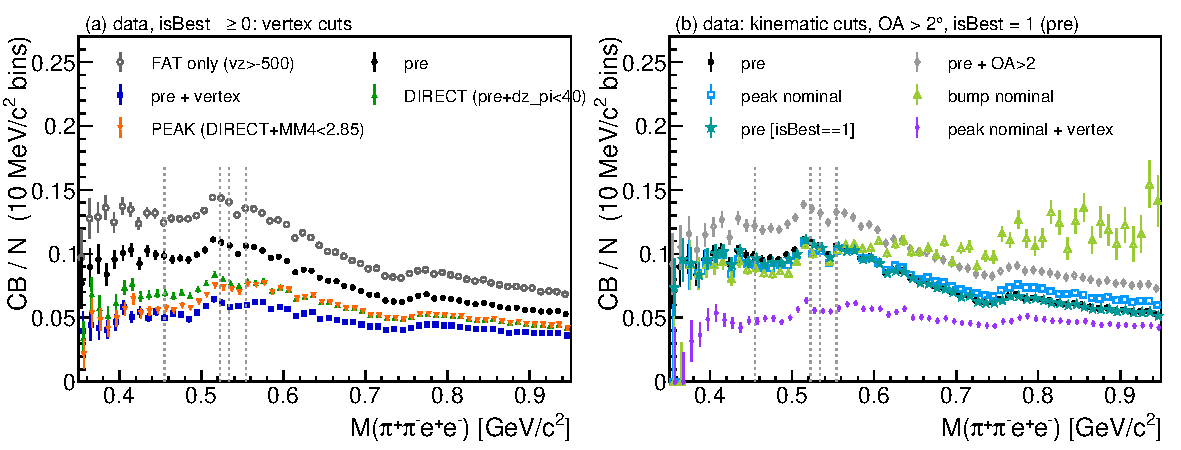
\includegraphics[width=\textwidth]{figs_exp/cb_share.pdf}
\caption{CB share CB$/N$ in 10\,\MeVcc bins of \Mfour, data, CB $=2\sqrt{N_{++}N_{--}}$, $k=1$. Selection: data; every curve has the \ptthreecap{}, a reconstructed event vertex ($\vz>-500$\,mm), particles identified by the START-free velocity \betanew (pions within $3\sigma$, leptons within $5\sigma$ of the expected band; leptons with a RICH ring) and energy-loss-corrected momenta for all four tracks; panel (a), all stored combinations of each event (isBest $\ge0$): nothing more (``FAT only''); in addition the target region $\vz>-160$\,mm (``pre''); ``pre'' and both pion tracks used in the fit of the event vertex (pre + vertex); ``pre'' and both pion tracks within 40\,mm of the event vertex along the beam ($\dzpi<40$\,mm) (DIRECT); DIRECT and missing mass $\MMfour<2.85$\,\GeVcc (PEAK); panel (b): ``pre''; ``pre'' and \ee opening angle OA$>2^\circ$; ``pre'' and angle between the \pipi and the \ee momenta in the laboratory $\alab<55^\circ$ and $\Mpipi>0.30$\,\GeVcc (peak nominal); ``pre'' and $\alab<40^\circ$, $0.30<\Mpipi<0.41$\,\GeVcc (bump nominal); ``pre'' with only the best-ranked combination of each event (isBest $=1$); peak nominal and both pion tracks used in the fit of the event vertex (peak nominal + vertex); the like-sign counts ($\pipi e^+e^+$, $\pipi e^-e^-$) of the CB pass the same cuts. Dotted: bump window
0.4550--0.5225 and peak window 0.53364--0.55416\,\GeVcc. (a) Vertex cuts, isBest $\ge0$: FAT only ($\vz>-500$\,mm),
``pre'' ($+\vz>-160$\,mm), pre + both pions in the vertex fit, DIRECT, PEAK. (b) ``pre'', pre + OA$>2^\circ$, peak
nominal, bump nominal, ``pre'' with isBest $=1$ (plain formula), peak nominal + vertex. Equal y ranges; not normalised
to luminosity.}
\label{fig:cb_share}
\end{figure}

\begin{figure}[!htbp]
\centering
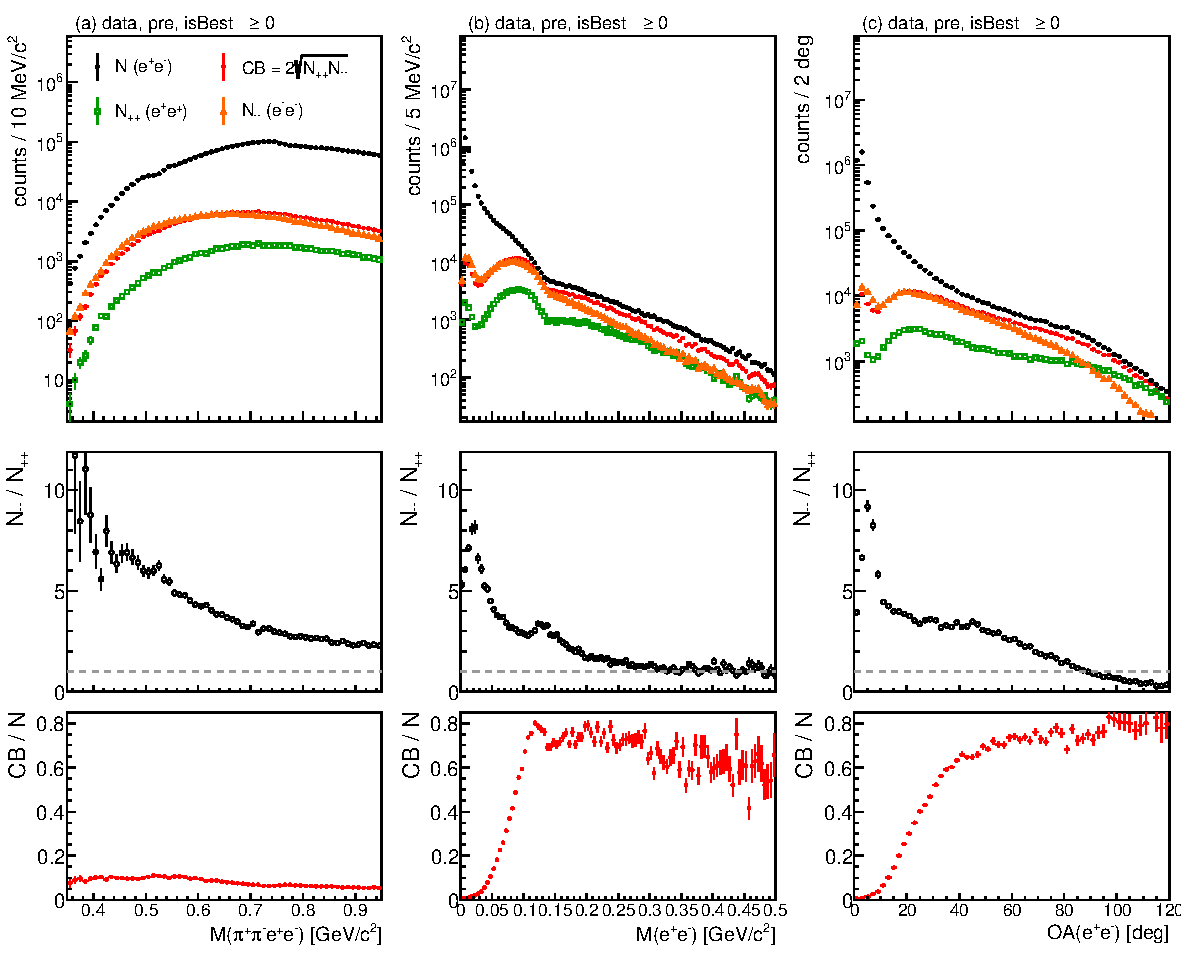
\includegraphics[width=\textwidth]{figs_exp/cb_spectra_cnt.pdf}
\caption{Like-sign counts and the CB, data, selection ``pre'' (all combinations isBest $\ge0$, \code{cor_ok} $=1$, PT3,
$\vz>-500$\,mm, $\vz>-160$\,mm). Selection: data with the base cuts \ptthreecap{}, an event vertex reconstructed ($\vz>-500$\,mm) and inside the target region ($\vz>-160$\,mm), particles identified by the START-free velocity \betanew (pions within $3\sigma$, leptons within $5\sigma$ of the expected band; leptons with a RICH ring), energy-loss-corrected momenta for all four tracks, all stored \ppee combinations of each event (isBest $\ge0$), no further cut (together called ``pre''); columns (b) and (c) contain the counts at every \Mfour; the like-sign counts ($\pipi e^+e^+$, $\pipi e^-e^-$) pass the same cuts. Columns: (a) \Mfour in 10\,\MeVcc bins; (b) \Mee in 5\,\MeVcc bins; (c) OA in
$2^\circ$ bins; (b) and (c) contain all counts at any \Mfour. Top (log scale): $N$ black, $N_{++}$ green squares,
$N_{--}$ orange triangles, CB $=2\sqrt{N_{++}N_{--}}$ red (per bin, no interpolation, $k=1$). Middle: $N_{--}/N_{++}$
(dashed: 1). Bottom: CB$/N$. Not normalised to luminosity.}
\label{fig:cb_spectra}
\end{figure}

\begin{figure}[!htbp]
\centering
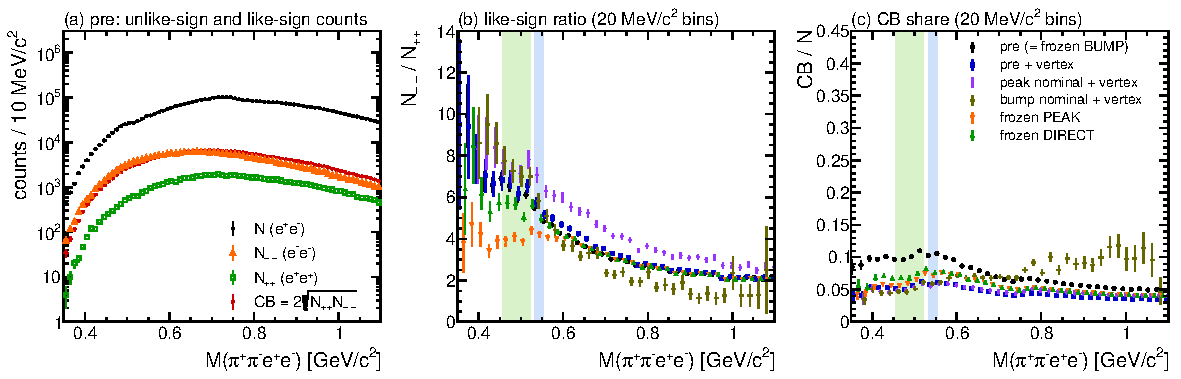
\includegraphics[width=\textwidth]{figs_exp/spec_likesign_cnt.pdf}
\caption{Like-sign composition, isBest $\ge0$. Selection: data with the base cuts \ptthreecap{}, an event vertex reconstructed ($\vz>-500$\,mm) and inside the target region ($\vz>-160$\,mm), particles identified by the START-free velocity \betanew (pions within $3\sigma$, leptons within $5\sigma$ of the expected band; leptons with a RICH ring), energy-loss-corrected momenta for all four tracks, all stored \ppee combinations of each event (isBest $\ge0$) (together called ``pre''); panel (a): ``pre'' alone; panels (b) and (c), the six selections of Fig.~\ref{fig:m4_overview}: ``pre'' ($=$ BUMP); ``pre'' and both pion tracks used in the fit of the event vertex (pre + vertex); ``pre'' and angle between the \pipi and the \ee momenta in the laboratory $\alab<55^\circ$, $\Mpipi>0.30$\,\GeVcc and both pions in the vertex fit (peak nominal + vertex); ``pre'' and $\alab<40^\circ$, $0.30<\Mpipi<0.41$\,\GeVcc and both pions in the vertex fit (bump nominal + vertex); ``pre'' and both pion tracks within 40\,mm of the event vertex along the beam ($\dzpi<40$\,mm) and $\MMfour<2.85$\,\GeVcc (PEAK); ``pre'' and $\dzpi<40$\,mm (DIRECT); the like-sign counts pass the same cuts. (a) ``pre'': $N$, $N_{--}$ (orange triangles), $N_{++}$ (green squares) and CB $=2\sqrt{N_{++}N_{--}}$ in
10\,\MeVcc bins. (b) $N_{--}/N_{++}$ against \Mfour (20\,\MeVcc bins, Poisson errors) for the six selections of
Fig.~\ref{fig:m4_overview} (one colour per selection, as in Fig.~\ref{fig:cb_share}). (c) CB$/N$ for the same selections. Bands: data windows.
Panel (a) repeats Fig.~\ref{fig:cb_spectra}(a) with the interpolated CB, for comparison with (b) and (c). FAT preselection and
\code{cor_ok} $=1$ applied; counts, not normalised to luminosity.}
\label{fig:spec_likesign}
\end{figure}

% spec_vertexcut_cnt.tex: copy of spec_vertexcut.tex with "rows" -> "counts" (analyst, 15 Nov 2026; Part II writer, integ4)
% written by plots/exp_report/spec_m4.C -- pass fractions of the counts under the vertex cuts, unlike-sign vs like-sign
\begin{table}[H]
\centering
\scriptsize
\caption{Pass fractions of the vertex cuts for the unlike-sign counts ($e^+e^-$) and the two like-sign hypotheses ($e^+e^+$, $e^-e^-$), all stored combinations ($\mathrm{isBest}\ge0$), corrected momenta, PT3, event vertex $z>-500$~mm (FAT). Base of $v_z>-160$~mm: $\mathrm{cor\_ok}=1$; base of the other two cuts: \emph{pre}. CB kept $=\sqrt{f_{++}f_{--}}$ (kept part of $2\sqrt{N_{++}N_{--}}$); the last column is the factor by which the cut lowers CB/$N$. Errors: statistical, with the event-group correlation (ratio estimator).}
\label{tab:spec_vertexcut}
\begin{tabular}{llrrrrr}
\toprule
cut & $M_4$ region & $f(e^+e^-)$ & $f(e^+e^+)$ & $f(e^-e^-)$ & CB kept & CB/$N$ factor \\
\midrule
$v_z>-160$~mm & bump window & $0.897\pm0.001$ & $0.662\pm0.007$ & $0.707\pm0.003$ & 0.684 & 0.763 \\
 & peak window & $0.901\pm0.001$ & $0.670\pm0.010$ & $0.717\pm0.004$ & 0.693 & 0.769 \\
 & all & $0.931$ & $0.705$ & $0.727$ & 0.716 & 0.769 \\
\midrule
both $\pi$ in vertex fit & bump window & $0.726\pm0.001$ & $0.396\pm0.009$ & $0.410\pm0.004$ & 0.403 & 0.555 \\
 & peak window & $0.722\pm0.002$ & $0.405\pm0.012$ & $0.423\pm0.005$ & 0.414 & 0.573 \\
 & all & $0.803$ & $0.516$ & $0.514$ & 0.515 & 0.641 \\
\midrule
$\Delta z_\pi<40$~mm & bump window & $0.812\pm0.001$ & $0.638\pm0.009$ & $0.552\pm0.004$ & 0.594 & 0.731 \\
 & peak window & $0.812\pm0.001$ & $0.641\pm0.012$ & $0.570\pm0.005$ & 0.604 & 0.744 \\
 & all & $0.868$ & $0.694$ & $0.653$ & 0.673 & 0.776 \\
\bottomrule
\end{tabular}
\end{table}


\begin{figure}[!htbp]
\centering
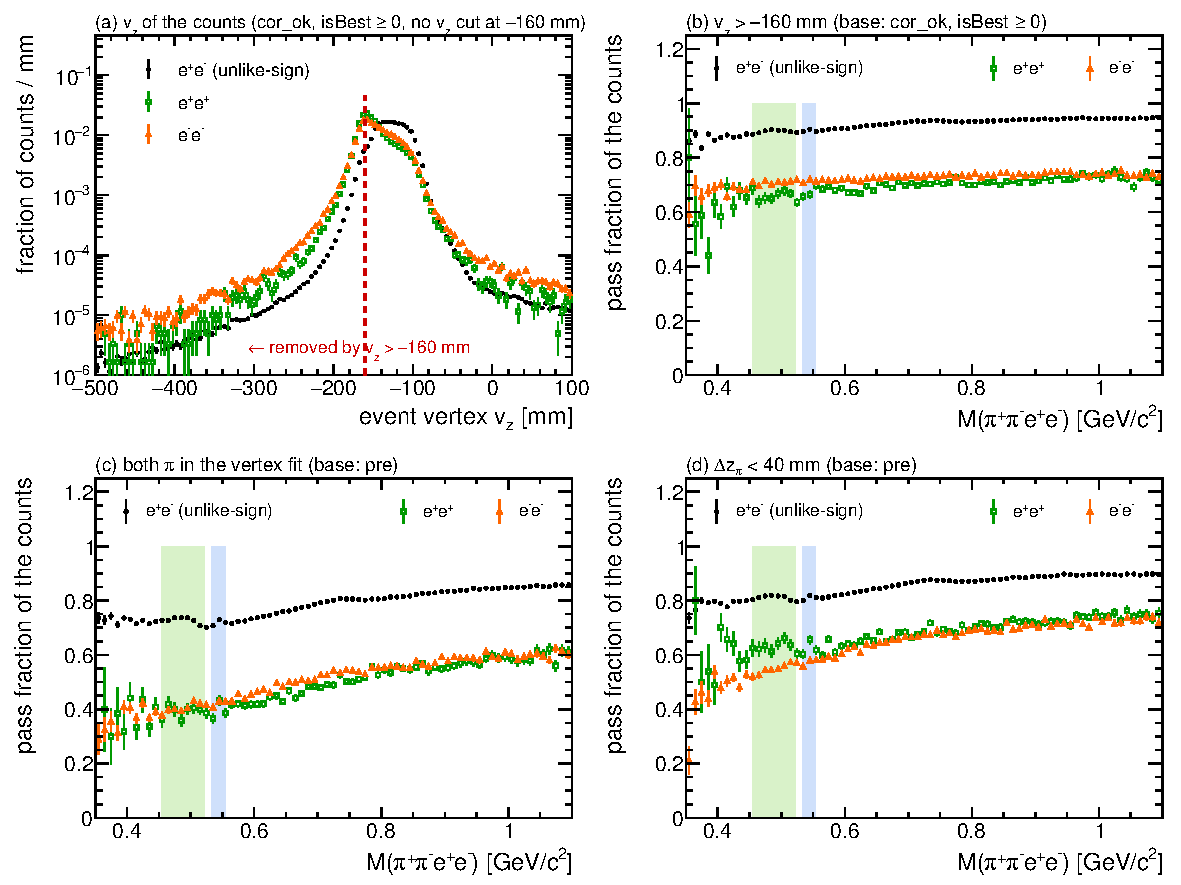
\includegraphics[width=\textwidth]{figs_exp/spec_vertexcut_cnt.pdf}
\caption{Effect of the analysis vertex cuts on unlike-sign (black) and like-sign (green squares $e^+e^+$, orange triangles $e^-e^-$)
counts; all combinations (isBest $\ge0$), corrected momenta, PT3, $\vz>-500$\,mm. Selection: data, \ptthreecap{}, a reconstructed event vertex ($\vz>-500$\,mm), particles identified by the START-free velocity \betanew (pions within $3\sigma$, leptons within $5\sigma$ of the expected band; leptons with a RICH ring), energy-loss-corrected momenta for all four tracks, all stored combinations of each event (isBest $\ge0$); panel (a) and the base of panel (b): nothing more (no target-region cut); base of panels (c) and (d): in addition $\vz>-160$\,mm (together ``pre''); cut tested: (b) $\vz>-160$\,mm, (c) both pion tracks used in the fit of the event vertex, (d) both pion tracks within 40\,mm of the event vertex along the beam ($\dzpi<40$\,mm); the like-sign counts pass the same cuts. (a) $\vz$ before the cut
$\vz>-160$\,mm (red), unit area per sample, 5\,mm bins. (b)--(d) Pass fraction of the counts against \Mfour (10\,\MeVcc bins) of
(b) $\vz>-160$\,mm (base \code{cor_ok} $=1$), (c) both pions in the vertex fit (base ``pre''), (d) $\dzpi<40$\,mm (base
``pre''). Errors with the event-group correlation (ratio estimator). Bands: data windows. Not normalised to luminosity.}
\label{fig:spec_vertexcut}
\end{figure}

\subsection{Null tests}
\label{sec:cbnull}
\textbf{Frozen $\eta$ fit on the like-sign spectra} (Poisson likelihood; Table~\ref{tab:cb_null}, Fig.~\ref{fig:cb_null}):
for ``pre'' $S(N_{++}+N_{--})=-56\pm132$ (pull $-0.43$), against $S=4671\pm367$ in $N-\mathrm{CB}$; for peak nominal + vertex
$59\pm78$; over all 21 tested selections the pulls lie between $-0.6$ and $+1.7$ (correlated, the selections share
counts). Moving the test Gaussian to 46 positions in 0.40--0.85\,\GeVcc gives pull means $-0.12$\dots$+0.03$ and rms
0.83--1.12: the like-sign spectra have no peak-like structure. A structure of the CB on the 10\,\MeVcc scale would
enter $S$ directly; these tests exclude it at about 130 counts (one standard deviation for ``pre''), 3\,\% of $S$.
\textbf{$N-\mathrm{CB}$ at 13 displaced positions} 0.575--0.695\,\GeVcc (``pre''): pull mean $-1.2$, rms 1.8 over all of
them, but the three largest pulls ($-2.5$, $-2.6$, $-4.2$ at 0.675--0.695) belong to fit ranges that reach 0.741--0.761\,\GeVcc,
where $N-\mathrm{CB}$ stops rising and turns over (maximum at 0.73--0.74\,\GeVcc, a drop of 15\,\% up to 0.78; visible in
Fig.~\ref{fig:res_overview}). This structure is most likely the kinematic edge of $\omega\to\pipi\piz$, $\piz\to\ee\gamma$ with
the photon lost (Eq.~(\ref{eq:m4max}) with $m_\omega$: 0.763\,\GeVcc on the measured scale at $\Mpipi=2m_\pi$, lower for larger
\Mpipi); this was not tested further. A pol2 cannot follow it. The ten positions 0.575--0.665, whose ranges end below
0.735\,\GeVcc, give pull mean $-0.63$ and rms 1.03 (\code{tables_exp/fix_checks.txt}, part C); since the like-sign spectra are smooth
there, the remaining small negative mean is a property of the physical background, not of the CB.
\textbf{Bump edge step on the like-sign counts}: $E_{\mathrm{ls}}=0.5\pm25.6$ (``pre''), $-6\pm14$ (bump nominal + vertex),
against $E=1199\pm71$ and $1004\pm51$ on $N-\mathrm{CB}$; per slice the like-sign heights are within $2.9\sigma$ of zero
(one slice, 0.37--0.39 of ``pre'', $-28.5\pm9.9$). The bump edge does not come from the CB; a single-slice
comparison is less clean than the sum.

\textbf{Later (Part~III, data only): the like-sign counts in the distance to the edge, $u$.} \emph{In short: in $u$ the $e^-e^-$ counts have a
step at the bump edge (4.7$\sigma$); it is made of lepton pairs from the two photons of the \piz in $\eta\to\pipi\piz$, lies at large \Mee, and
the CB subtracts these pairs from the unlike-sign counts as designed; it is not a charge flip. Confirmed by an independent verifier (wording corrected below).}
In $u=\Mfour-\Medge(\Mpipi,\Mee)$ (\S\ref{sec:edgeu}; ``pre'' + vertex, $0.30\le\Mpipi<0.40$\,\GeVcc) the like-sign counts alone were fitted with
the step fit of the unlike-sign counts (second-order polynomial + step at $u=0$, $-45\le u<+45$\,\MeVcc; Fig.~\ref{fig:res-edgeu}c). The
$e^+e^+$ counts show $2.1\pm6.5$ counts per 2.5\,\MeVcc over all \Mee; the $e^-e^-$ counts show $73.5\pm15.7$ (4.7$\sigma$; $\chi^2/\mathrm{ndf}=37.1/32$
with the step); their sum gives $75.7\pm17.0$. Through CB $=2\sqrt{N_{++}N_{--}}$ the subtracted CB carries 39 counts of step, 3.0\,\% of the
unlike-sign step $h_u$; Part~III counts it in its CB systematic (2.6\,\%). Two features noted at first are not significant: 91.5\,\% of the
$e^-e^-$ counts in the fit range have $\Mee\ge10$\,\MeVcc, so ``only above 10\,\MeVcc'' ($78.7\pm15.0$ against $-5.4\pm4.6$; an even share would
put 6 counts below, a 2.6$\sigma$ deficit) mostly reflects the distribution of the counts; and the periods (I $50.8\pm10.8$, IIA $1.0\pm3.9$, IIB
$7.3\pm6.9$, III $14.7\pm8.2$) agree with a share that follows the luminosity ($\chi^2/\mathrm{ndf}=4.9/3$, $p=0.18$).

\emph{The study of the step} (Part~III, package eestep, and its independent verification, package veestep; data side). Every like-sign entry and the unlike-sign entries near the edge were joined to their
PAT entries (551\,291 entries, momenta identical), which gives the track quality of each lepton and the lepton multiplicities of the event; the
$e^+e^-$, $e^+e^+$ and $e^-e^-$ entries of one event were linked by a key of run number, event counter, START time, vertex $z$ and total
multiplicity (every key one block of adjacent entries, no exception). Findings:
\begin{itemize}\setlength{\itemsep}{0pt}
\item \emph{The mechanism.} In $\eta\to\pipi\piz$ a lepton pair can be made of leptons from the two \emph{different} photons of the \piz (a Dalitz
      lepton and a conversion lepton of the other photon, or one conversion lepton of each). Kinematics gives such pairs, at a given \Mee,
      exactly the largest \Mfour of the bump, $\Medge(\Mpipi,\Mee)$: the verifier proved it for any pair of \piz decay products with the rest
      lost (Compton electrons of a photon included), and two toys ($4\times10^5$ and $6\times10^5$ decays per topology) never exceed $u=0$. The
      pairs near this limit are heavy (median \Mee 113--128\,\MeVcc). Near the limit their density falls over the last 5--10\,\MeVcc, so after
      the resolution their step sits at $u\approx-2.5$\,\MeVcc (verifier's toy; 0 for the bump itself), where the data put it (next items).
\item \emph{The step sits at large \Mee} (Fig.~\ref{fig:cb-eestep-spec}): $e^-e^-$ $3.6\pm8.9$ counts below 50\,\MeVcc (where 90\,\% of the bump
      lies), $13.0\pm9.1$ at 50--90 and $57.0\pm9.1$ (6.3$\sigma$) at \Mee$\ge90$\,\MeVcc. By opening angle of the two $e^-$: $-8.1\pm7.1$
      at 0--10$^\circ$, $9.1\pm6.0$ at 10--20$^\circ$, $25.1\pm8.7$ at 20--35$^\circ$, $40.9\pm8.5$ at 35--60$^\circ$, $5.9\pm3.3$ above; the bump
      step of $N$ is at 0--10$^\circ$ (1170 of 1349 counts).
\item \emph{It is tied to the edge with its \Mee term} ($e^-e^-$, \Mee$\ge70$\,\MeVcc; Fig.~\ref{fig:cb-eestep-align}): $\Delta\chi^2$ of the
      step 28.3 in $u$, 0.5 with the edge at $\Mee\to0$ (the measure $E$ of this report), 10.3 at a fixed $\Mfour=0.535$\,\GeVcc, 3.5 and 19.8
      with the edge moved by $\mp10$\,\MeVcc; a free step position gives $u_0=-2.5$\,\MeVcc ($u_0=0$: $+2.0$ in $\chi^2$, $+5$\,\MeVcc:
      $+13.4$). It grows toward the high \Mpipi slice ($8.7\pm6.7$, $17.8\pm6.4$, $30.9\pm6.4$) and is absent where the decay is impossible
      (\Mpipi 0.42--0.46\,\GeVcc: $-2.0\pm3.1$). This is why \Mfour per slice shows no like-sign step ($0.5\pm25.6$): at large \Mee the true edge
      lies far below the edge at $\Mee\to0$.
\item \emph{Events without an $e^+$.} 85\,\% of the $e^-e^-$ counts near the edge come from events with no positive lepton and no $e^+e^-$ count; the
      step is there ($66.4\pm14.5$). Events with an $e^+e^-$ ``twin'' (same $\pi^+$, $\pi^-$ and one of the two $e^-$) show none ($6.8\pm6.0$);
      nor do counts whose two $e^-$ share a RICH ring ($-2.7\pm4.7$) or events with three or more $e^-$ ($0.6\pm2.8$). A conversion pair merged
      into one track would carry the whole photon and double the ring and the energy loss in the MDC; the step counts show no such excess
      (verifier: share of the step in the top third of these variables 0.30--0.36).
\item \emph{Ordinary tracks.} The share of step counts is flat in every track-quality variable (RK, inner and outer segment, META and RICH match,
      ring pads, $\beta$, momenta; $p=0.14$--0.99), in the sectors (0.30--0.47; sector~2: 0.39) and in the days ($p=0.26$).
\item \emph{$e^+e^+$ too.} At \Mee$\ge90$\,\MeVcc the $e^+e^+$ counts step by $7.3\pm4.3$ counts, a ratio $e^+e^+/e^-e^-$ of $0.13\pm0.08$: soft $e^+$
      are accepted less often than soft $e^-$, and a photon can also give a Compton or knock-on electron, which is always negative (SMASH
      contains such pairs, mostly $e^-e^-$; the simulation is used here for the origin only). ``The $e^+e^+$ counts show no step'' was a statement
      about small numbers. These pairs are one of the correlated $e^-e^-$ sources behind $N_{--}/N_{++}=5.4$ of the like-sign counts
      (\S\ref{sec:cbshare}).
\item \emph{Not a charge flip.} A Dalitz $e^+$ reconstructed as $e^-$ keeps its momentum, so the $e^-e^-$ count would have the small \Mee of the
      bump; there the step is $3.6\pm8.9$ counts against 1209.7 counts of bump step in $N$: flip rate $r=0.003\pm0.007$, $r<1.24$\,\% (90\,\% CL).
      Unlike-sign counts with an $e^-e^-$ twin (a wrong-sign copy of the $e^+$) show no step ($-4.1\pm7.4$; verifier, with the second $e^-$
      within 3$^\circ$ of the $e^+$: $-4.8\pm3.1$).
\item \emph{The CB subtracts these pairs as designed.} A decay with a Dalitz or conversion pair on each photon gives one $e^-e^-$, one
      $e^+e^+$ and two $e^+e^-$ cross pairs; a Compton or knock-on electron gives one $e^-e^-$ and one $e^+e^-$ pair. The $e^+e^-$ ones are in $N$;
      with an acceptance that factorises per lepton the CB rule removes both kinds to within a few per cent (expected $k$ 0.96--1.02). At
      \Mee$\ge90$\,\MeVcc, where the bump is small, $N$ steps by $52.6\pm10.9$ counts, the CB by $35.8\pm8.6$, and $N-\mathrm{CB}=16.8\pm13.9$
      (Fig.~\ref{fig:res-eestep}b; verifier, with its own CB construction: $52.7\pm10.4$, $39.6\pm9.8$, $13.1\pm14.6$). Part~III compares this with
      the bump signal expected there, SMASH $\times f$ with the per-count C2 weights of D38 (16.9 counts: $z=-0.01$; a like-sign artefact
      without $e^+e^-$ partners would give $-19.0$, 2.6$\sigma$ away, statistical; about 2.3$\sigma$ with the error of the simulated prediction,
      $\pm6.7$); $k_{\mathrm{cross}}=1.00\pm0.39$ (independent check, still with the earlier constant C2 factors: $0.96\pm0.48$).
\item \emph{Peak and X17 windows.} The cross pairs reach the peak window only for \Mee$\ge101.5$--119.5\,\MeVcc (\Mpipi 0.28--0.40\,\GeVcc);
      with the share of cross pairs just below the edge ($0.56\pm0.09$) there are about 180 in the lower side band (0.5250--0.5336\,\GeVcc;
      255 in 0.5225--0.5336) and about 50 in the peak window, subtracted with their partners, so the peak content is unchanged (residual below
      1.5 counts with the expected $k$). For \Mee$\le24.5$\,\MeVcc their edge is at most 0.5211--0.5223\,\GeVcc, 11--12.5\,\MeVcc below the peak
      window: none of the 207 $e^-e^-$ and 13 $e^+e^+$ counts of the X17 window can be a cross pair, and the $e^-e^-$ step
      at 10--30\,\MeVcc is $4.2\pm5.8$.
\end{itemize}
\emph{Meaning:} the step is physics of the $\eta$ decay, not a detector artefact; the CB rule handles it, the $\eta$-peak results and the X17
band do not depend on it, and the bump step contains it only as the 3\,\% that the CB correctly carries. The earlier caveat (the bump scale of
Part~III up to about 8\,\% higher through a wrong charge sign) is withdrawn; Part~III quotes at most $+1.6$\,\% from an $e^+\to e^-$ flip
(1.9\,\% for either charge; 90\,\% CL).
\emph{Status:} measured (Part~III, package edgeu, confirmed by an independent verifier); mechanism found by the package eestep and confirmed by
an independent verifier with own code (package veestep; wording corrected as above); D39 (record the origin, keep the CB) approved by the analyst on
15 November 2026. No merged conversion pairs are seen; the CB comes from the data.

\begin{figure}[!htbp]
\centering
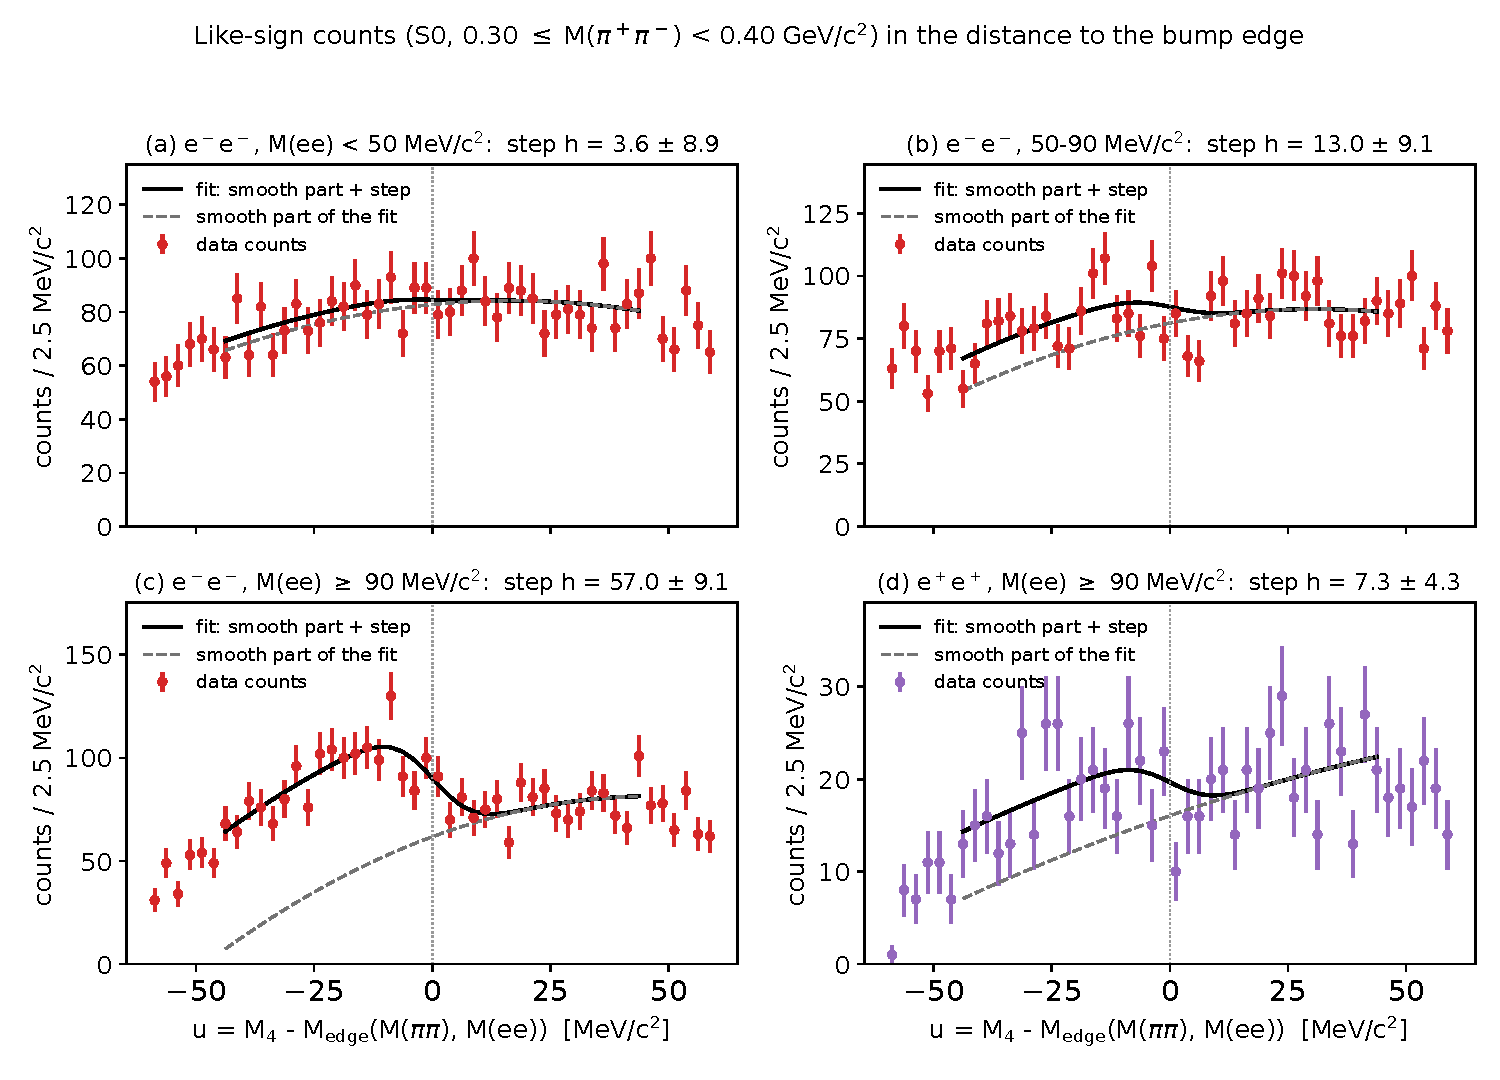
\includegraphics[width=0.92\textwidth]{figs_exp/p12w_eestep_spectra_cnt.pdf}
\caption{\textbf{What it shows: the like-sign counts have no step at the bump edge below \Mee$=50$\,\MeVcc, where the bump lies, and a clear step at
\Mee$\ge90$\,\MeVcc, where the pairs from the two \piz photons lie, in $e^-e^-$ and (smaller) in $e^+e^+$.} Selection: data only, base cuts \ptthreecap{}, an event vertex reconstructed ($\vz>-500$\,mm) and inside the target region ($\vz>-160$\,mm), particles identified by the START-free velocity \betanew (pions within $3\sigma$, leptons within $5\sigma$ of the expected band; leptons with a RICH ring), energy-loss-corrected momenta for all four tracks, all stored \ppee combinations of each event (isBest $\ge0$) (together ``pre'') and both pion tracks used in the fit of the event vertex (``pre'' + vertex, called S0 in Part~III); $0.30\le\Mpipi<0.40$\,\GeVcc; like-sign counts only, no CB subtracted: $e^-e^-$ in (a)--(c), $e^+e^+$ in (d); $u$ is defined only for \Mee below the \piz mass (135\,\MeVcc), so the classes are (a) $\Mee<50$\,\MeVcc, (b) $50\le\Mee<90$\,\MeVcc, (c) and (d) $90\le\Mee<135$\,\MeVcc; fits in $-45\le u<+45$\,\MeVcc.
Data only, ``pre'' + vertex (``S0''), $0.30\le\Mpipi<0.40$\,\GeVcc, counts per 2.5\,\MeVcc in $u=\Mfour-\Medge(\Mpipi,\Mee)$. (a) $e^-e^-$,
\Mee$<50$\,\MeVcc: $3.6\pm8.9$; (b) $e^-e^-$, 50--90\,\MeVcc: $13.0\pm9.1$; (c) $e^-e^-$, \Mee$\ge90$\,\MeVcc: $57.0\pm9.1$; (d) $e^+e^+$,
\Mee$\ge90$\,\MeVcc: $7.3\pm4.3$. Points: data counts; black line: the fit (smooth part $+$ step, $\pm45$\,\MeVcc); grey dashed: the smooth part of
the same fit (it also absorbs the slope below the edge). Package eestep (\code{plots/all_report/eestep_figs.py}; axis label \Medge:
\code{p12w_partII_figs.py}).}
\label{fig:cb-eestep-spec}
\end{figure}

\begin{figure}[!htbp]
\centering
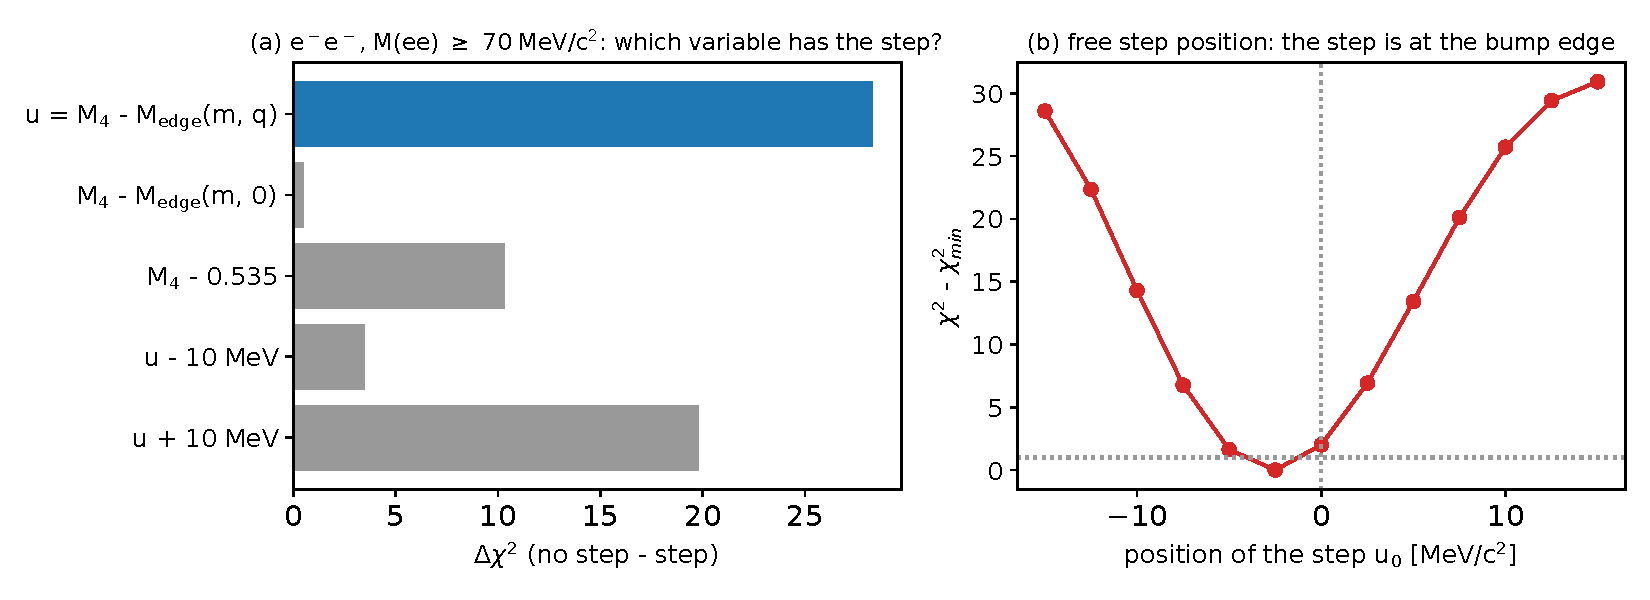
\includegraphics[width=0.92\textwidth]{figs_exp/p12w_eestep_align.pdf}
\caption{\textbf{What it shows: the $e^-e^-$ step follows the edge $\Medge(\Mpipi,\Mee)$ including its \Mee term and sits at $u=0$; with the edge at
$\Mee\to0$ (the measure $E$ of this report) or at a fixed \Mfour it is not seen.} Selection: data only, base cuts \ptthreecap{}, an event vertex reconstructed ($\vz>-500$\,mm) and inside the target region ($\vz>-160$\,mm), particles identified by the START-free velocity \betanew (pions within $3\sigma$, leptons within $5\sigma$ of the expected band; leptons with a RICH ring), energy-loss-corrected momenta for all four tracks, all stored \ppee combinations of each event (isBest $\ge0$) (together ``pre'') and both pion tracks used in the fit of the event vertex; $0.30\le\Mpipi<0.40$\,\GeVcc; only the like-sign $e^-e^-$ counts with $70\le\Mee<135$\,\MeVcc (\Mee below the \piz mass, where $u$ is defined), no CB; each of the five variables fitted from $-45$ to $+45$\,\MeVcc.
Data only, ``pre'' + vertex, $e^-e^-$ counts with \Mee$\ge70$\,\MeVcc, $0.30\le\Mpipi<0.40$\,\GeVcc. (a) $\Delta\chi^2$ between the fits without and
with a step for five variables: $u$ (28.3), $\Mfour-\Medge(m,0)$ (0.5), $\Mfour-0.535$\,\GeVcc (10.3), and the edge moved by $-10$ and
$+10$\,\MeVcc (3.5, 19.8). (b) $\chi^2-\chi^2_{\min}$ against the step position $u_0$: minimum at $-2.5$\,\MeVcc, where the independent
verifier's toy puts the step of these pairs; dotted: $\Delta\chi^2=1$. Package eestep (axis labels \Medge: \code{p12w_partII_figs.py}).}
\label{fig:cb-eestep-align}
\end{figure}

% cb_null_cnt.tex: copy of cb_null.tex with "rows" -> "counts" (analyst, 15 Nov 2026; Part II writer, integ4)
% written by plots/exp_report/cb_checks.C
\begin{table}[H]\centering\footnotesize\setlength{\tabcolsep}{3pt}
\caption{Null tests of the like-sign spectra, experimental data, isBest $\geq 0$ unless marked. $S$ = $\eta$-peak content from $P_\text{main}$ ($N-\text{CB}$, frozen Gaussian 0.5439~GeV/$c^2$, $\sigma=5.4$~MeV, pol2, 0.5225--0.6100) with stat.\ error. $S(++)$, $S(--)$, $S(\Sigma)$: the same frozen fit (Poisson likelihood) on $N_{++}$, $N_{--}$ and $N_{++}+N_{--}$. Pulls: mean and rms of $S/\sigma_S$ of $N_{++}+N_{--}$ for the test Gaussian at 46 positions 0.40--0.85~GeV/$c^2$. $E$: bump edge-step sum on $N-\text{CB}$; $E_\text{ls}$: the same fit on $N_{++}+N_{--}$ (counts per 2.5~MeV/$c^2$). Not normalised to luminosity.}
\label{tab:cb_null}
\resizebox{\textwidth}{!}{%
\begin{tabular}{lrrrrrr}
\toprule
selection & $S$ & $S(++)$ & $S(--)$ & $S(\Sigma)$ & pulls mean/rms & $E$ / $E_\text{ls}$\\
\midrule
FAT only (vz$>$-500) & $4657\pm390$ & $-7\pm64$ & $-82\pm143$ & $-89\pm156$ & $-0.04$ / $1.00$ & $1241\pm76$ / $3\pm30$\\
pre & $4671\pm367$ & $-42\pm52$ & $-15\pm121$ & $-56\pm132$ & $-0.04$ / $0.96$ & $1199\pm71$ / $0\pm26$\\
pre + OA$>$2 & $3632\pm328$ & $-38\pm52$ & $-5\pm119$ & $-43\pm130$ & $-0.04$ / $0.98$ & $898\pm64$ / $1\pm25$\\
pre + vertex & $4388\pm307$ & $23\pm33$ & $36\pm79$ & $59\pm85$ & $-0.01$ / $1.07$ & $1142\pm59$ / $3\pm16$\\
DIRECT (pre+dz\_pi$<$40) & $4492\pm327$ & $50\pm42$ & $18\pm91$ & $66\pm100$ & $-0.03$ / $1.00$ & --\\
PEAK (DIRECT+MM4$<$2.85) & $4364\pm310$ & $20\pm40$ & $28\pm81$ & $47\pm91$ & $0.01$ / $0.98$ & --\\
peak nominal & $4330\pm327$ & $-53\pm43$ & $-16\pm111$ & $-70\pm119$ & $-0.05$ / $1.08$ & --\\
peak nominal + vertex & $3949\pm276$ & $14\pm28$ & $44\pm73$ & $59\pm78$ & $-0.01$ / $1.09$ & $1089\pm57$ / $6\pm16$\\
bump nominal & $2635\pm237$ & $16\pm33$ & $37\pm77$ & $51\pm84$ & $-0.12$ / $1.11$ & $1082\pm60$ / $0\pm21$\\
bump nominal + vertex & $2405\pm200$ & $25\pm22$ & $58\pm52$ & $84\pm56$ & $-0.07$ / $1.12$ & $1004\pm51$ / $-6\pm14$\\
pre [isBest=1] & $4199\pm330$ & $-58\pm47$ & $52\pm108$ & $-6\pm117$ & $-0.03$ / $0.95$ & $1050\pm64$ / $-28\pm23$\\
\bottomrule
\end{tabular}}
\end{table}


\begin{figure}[!htb]
\centering
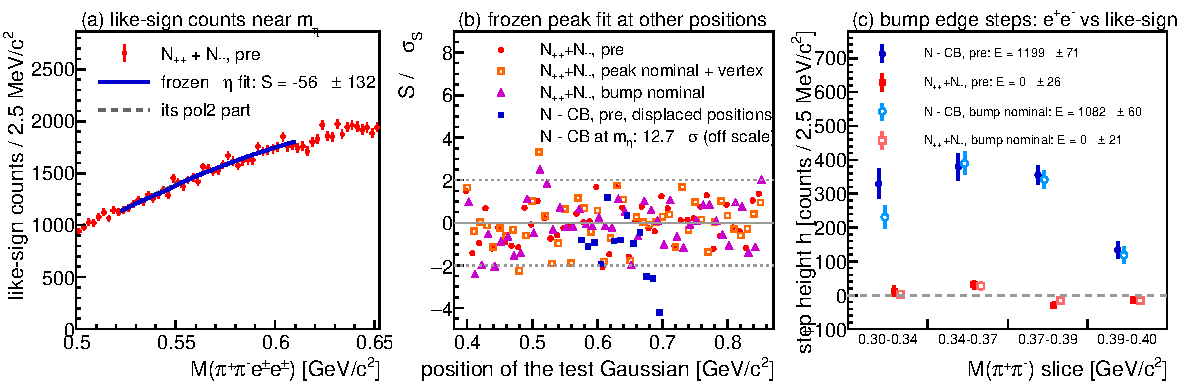
\includegraphics[width=\textwidth]{figs_exp/cb_null_cnt.pdf}
\caption{Null tests of the like-sign spectra, data, isBest $\ge0$. Selection: data with the base cuts \ptthreecap{}, an event vertex reconstructed ($\vz>-500$\,mm) and inside the target region ($\vz>-160$\,mm), particles identified by the START-free velocity \betanew (pions within $3\sigma$, leptons within $5\sigma$ of the expected band; leptons with a RICH ring), energy-loss-corrected momenta for all four tracks, all stored \ppee combinations of each event (isBest $\ge0$) (together ``pre''); (a) ``pre''; (b) the like-sign sum for ``pre'', for peak nominal + vertex (``pre'' and angle between the \pipi and the \ee momenta in the laboratory $\alab<55^\circ$, $\Mpipi>0.30$\,\GeVcc and both pion tracks used in the fit of the event vertex) and for bump nominal (``pre'' and $\alab<40^\circ$, $0.30<\Mpipi<0.41$\,\GeVcc), and $N-\mathrm{CB}$ for ``pre''; (c) ``pre'' and bump nominal in the four \Mpipi slices 0.30--0.34, 0.34--0.37, 0.37--0.39 and 0.39--0.40\,\GeVcc. (a) $N_{++}+N_{--}$ near $m_\eta$, ``pre'', with
the frozen $\eta$ fit (Gaussian 0.5439\,\GeVcc, 5.4\,\MeVcc + pol2, 0.5225--0.6100, Poisson likelihood): $S=-56\pm132$,
while $N-\mathrm{CB}$ gives $4671\pm367$. (b) $S/\sigma_S$ of the same fit moved with its range: $N_{++}+N_{--}$ at 46
positions 0.40--0.85\,\GeVcc for ``pre'', peak nominal + vertex and bump nominal; $N-\mathrm{CB}$ at 13 positions
0.575--0.695 (blue squares, ``pre''; the three lowest, at 0.675--0.695, have fit ranges that reach the turnover of $N-\mathrm{CB}$ near
0.74\,\GeVcc, \S\ref{sec:cbnull}); the value at $m_\eta$ (12.7) is off scale and given in the legend. (c) Bump
edge-step heights per \Mpipi slice on $N-\mathrm{CB}$ (blue) and on $N_{++}+N_{--}$ with the same fixed edges (red), for
``pre'' and bump nominal; counts per 2.5\,\MeVcc. Not normalised to luminosity.}
\label{fig:cb_null}
\end{figure}

\subsection{isBest and the CB}
\label{sec:cbisbest}
To see how isBest acts on the CB, the three trees were joined per event (key \code{file_id}, run, event number and
the stored vertex): 4\,058\,586 \ee events, no duplicated keys; 29.8\,\% of the $e^+e^+$ and 18.9\,\% of the $e^-e^-$
events also have \ee counts; only 1.5\,\% of the ``pre'' \ee events have three or more leptons. The like-sign formula
splits into the lepton classes $n=2$, 3, $\ge4$ as 0.745/0.222/0.033 (peak window); summed per class it equals the
plain formula within 0.5\,\%.

\textbf{Direct test} (bump window, class 3): the \ee counts keep 0.414 under isBest $=1$, the like-sign formula 0.724,
ratio 0.57, close to the 1/2 expected for two competing hypotheses (class 4: 0.228 against 0.533; class 2: 0.824
against 0.811, where only the pion combinations compete). The plain formula on isBest $=1$ counts gives a negative
$N-\mathrm{CB}$ in class 3 ($-195$ counts).

\textbf{Expected excess.} If each competing lepton hypothesis is chosen equally often, the plain formula on
isBest $=1$ counts is too high by $X=\sum\mathrm{GM}_c/\sum\varepsilon_c\mathrm{GM}_c$ with $\varepsilon=1$, 1/2, 1/4 for the
classes: $X=1.158$ (bump window), 1.157 (peak window), 1.167 (0.35--0.95\,\GeVcc); with the isBest $=1$ like-sign counts
themselves 1.14; 1.172 in 0.60--0.70\,\GeVcc. In this channel the excess is therefore \emph{expected} to be 14--17\,\%
(the \ee channel had 22\,\%), if each competing hypothesis is chosen equally often; the class-3 test above (ratio 0.57,
close to 1/2) supports this, but it is not verified otherwise. Scaling CB(isBest $=1$)
by 0.87 changes $S$ by $-0.2$ to $+0.3$\,\% and $W$ by $+0.7$ to $+1.8$\,\%; CB$/N$ (isBest $=1$) becomes 0.087 (peak)
and 0.086 (bump). The simulation study of the \ee channel (quoted only for this isBest question, never for a CB number) gave a ratio
formula/true CB of 1.21 for isBest $=1$ and 0.94--1.0 for all combinations. The equal-probability model is
not verified for the four-track time $\chi^2$; it is not needed for the main variant.

\textbf{Content ratio.} $S(\text{isBest}=1)/S(\text{isBest}\ge0)=0.899$ (``pre''), 0.900 (peak nominal), 0.912 (peak
nominal + vertex) at about the same $F$ (Fig.~\ref{fig:spec_m4_isbest}). With the event-group term in the errors of the
main variant (isBest $=1$ has none) isBest $=1$ is at least as precise: $F_g=12.54$ against 12.74 (``pre''), 13.94 against
14.44 (PEAK). The additional combinations add about 10\,\% signal but no precision.

\begin{figure}[!htb]
\centering
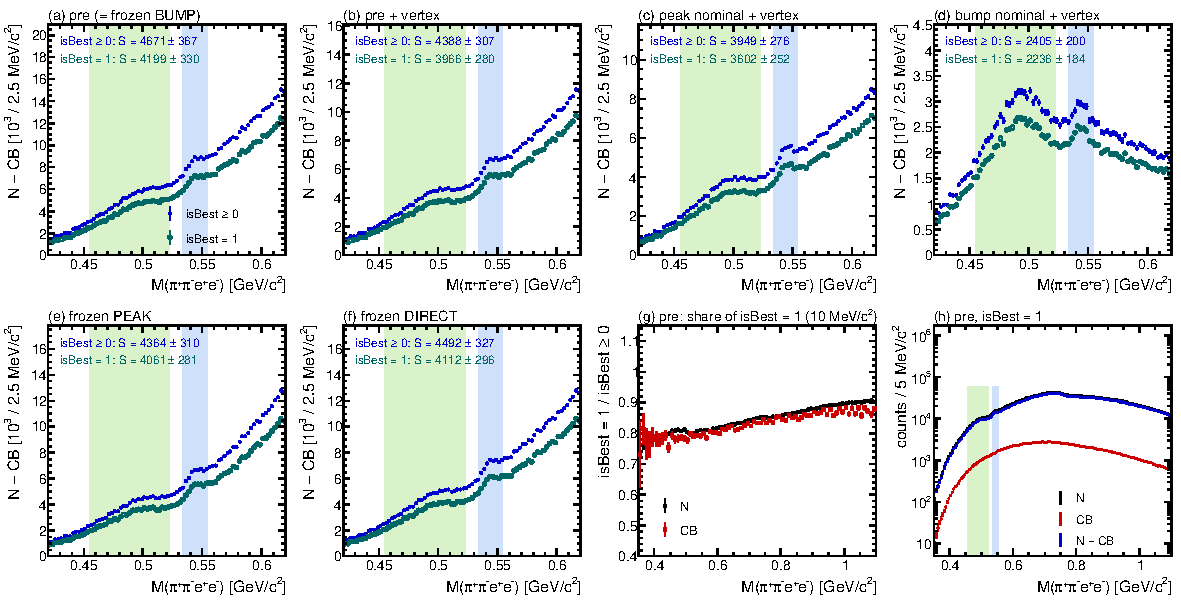
\includegraphics[width=\textwidth]{figs_exp/spec_m4_isbest_cnt.pdf}
\caption{All stored combinations (isBest $\ge0$, full blue) against one combination per event (isBest $=1$, open
cyan). Selection: data, \ptthreecap{}, an event vertex reconstructed ($\vz>-500$\,mm) and inside the target region ($\vz>-160$\,mm), particles identified by the START-free velocity \betanew (pions within $3\sigma$, leptons within $5\sigma$ of the expected band; leptons with a RICH ring), energy-loss-corrected momenta for all four tracks, each with all stored combinations (isBest $\ge0$; with these cuts: ``pre'') or only the best-ranked combination of each event (isBest $=1$); in addition (a) nothing, (b) both pion tracks used in the fit of the event vertex, (c) angle between the \pipi and the \ee momenta in the laboratory $\alab<55^\circ$, $\Mpipi>0.30$\,\GeVcc and both pions in the vertex fit, (d) $\alab<40^\circ$, $0.30<\Mpipi<0.41$\,\GeVcc and both pions in the vertex fit, (e) both pion tracks within 40\,mm of the event vertex along the beam ($\dzpi<40$\,mm) and $\MMfour<2.85$\,\GeVcc, (f) $\dzpi<40$\,mm; (g), (h) nothing (``pre''); the like-sign counts pass the same cuts. (a)--(f): $N-\mathrm{CB}$ in 0.42--0.62\,\GeVcc for the six selections of Fig.~\ref{fig:m4_overview}, with the
\Pmain $S$ of both variants (common y range within a panel). (g) ``pre'': share of isBest $=1$ counts in $N$ (black) and
in the CB (red) against \Mfour, 10\,\MeVcc bins. (h) ``pre'', isBest $=1$: $N$, CB, $N-\mathrm{CB}$ (5\,\MeVcc, log scale).
CB $=2\sqrt{N_{++}N_{--}}$, $k=1$ (plain formula also for isBest $=1$). Counts, not normalised to luminosity.}
\label{fig:spec_m4_isbest}
\end{figure}

\subsection{Sensitivity of the results to the CB}
\label{sec:cbsens}
The CB was changed on the filled spectra in ten ways and $S$ (\Pmain), $E$ and $W$ were recomputed
(Table~\ref{tab:cb_sens}, Fig.~\ref{fig:cb_sensitivity}):
\begin{itemize}
\setlength{\itemsep}{0pt}
\item CB$\times0.97$ and $\times1.03$: $S$ changes by at most 0.07\,\% (3 counts), $E$ by at most 0.1\,\%; $W$ by
      $\pm0.1$--0.5\,\% ($=3\,\%\times\mathrm{CB}/(N-\mathrm{CB})$). For scale factors 0.90--1.10, $S$ moves by at most
      0.23\,\% and $E$ by 0.36\,\%.
\item CB bins of 2.5, 5, 20\,\MeVcc instead of 10: $S$ $-1.6$\dots$+2.1$\,\% (X17: $-2.6$\,\%), $E$ up to $+1.8$\,\%; mostly
      the statistical noise of the CB estimate, inside the 7--9\,\% statistical error of $S$; not to be added again.
\item step or cubic instead of linear interpolation: $S$ $-0.6$\dots$+0.1$\,\%.
\item CB$\times k_{\mathrm{mix}}(\Mfour)$ of the selection: $S$ $-0.1$\dots$+0.6$\,\%, $E$ 0\dots$+0.7$\,\%, $W$
      $-0.1$\dots$-0.4$\,\%.
\item like-sign sum shape normalised to the geometric mean, and the plain sum $N_{++}+N_{--}$: not valid estimators
      (the like-sign ratio changes from 7 to 2.3 across \Mfour); $W$ moves by up to $-7.0$\,\%.
\end{itemize}
$S$ and $E$ hardly react because the free pol2 of the fits absorbs a smooth change of the CB; only $W$ follows the CB
directly. The largest of the scale, $k_{\mathrm{mix}}$ and interpolation effects is $\le0.6$\,\% for $S$ and $\le0.7$\,\% for
$E$. Because the normalisation of the CB is not known (correlated $e^-e^-$ sources, \S\ref{sec:cbshare}), the robust bound
is the plain sum $N_{++}+N_{--}$, a CB larger by 38--45\,\%: it changes $S$ by at most 1\,\% (X17 band and isBest $=1$ up to
2.3\,\%), $E$ by at most 3\,\% and $W$ by up to $-7$\,\%. CB$/N$ and $W$ therefore carry an unknown scale of this size.

% cb_sens_fl.tex: copy of cb_sens.tex as a page float [p] instead of [H] (Part II writer, integ4, 15 Nov 2026: avoids a nearly empty page)
% written by plots/exp_report/cb_checks.C
\begin{table}[p]\centering\footnotesize\setlength{\tabcolsep}{2.2pt}
\caption{Change of the $\eta$-peak content $S$ ($P_\text{main}$) and of the bump edge-step sum $E$, in per cent, when the CB is changed; experimental data, isBest $\geq 0$ unless marked. Columns: CB scaled by 0.97 and 1.03; CB bins of 2.5, 5 and 20~MeV/$c^2$ instead of 10; step and cubic instead of linear interpolation; CB multiplied by the event-mixing $k(M)$ of the selection (Table~\ref{tab:cb_kmix}; n/a: none made); like-sign sum shape normalised to the integrated geometric mean; plain like-sign sum $N_{++}+N_{--}$ (extreme, not an estimator). Last columns: statistical error and model spread of $S$ (of $E$: stat.\ only), in per cent. Not normalised to luminosity.}
\label{tab:cb_sens}
\resizebox{\textwidth}{!}{%
\begin{tabular}{lrrrrrrrrrrrr}
\toprule
selection & $\times0.97$ & $\times1.03$ & 2.5 & 5 & 20 & step & cubic & $k_\text{mix}$ & LS shape & $N_{++}+N_{--}$ & stat & spread\\
\midrule
\multicolumn{13}{l}{$\eta$-peak content $S$:}\\
FAT only (vz$>$-500) & -0.0 & +0.0 & +0.8 & +0.2 & -1.0 & -0.1 & -0.1 & n/a & +0.5 & +0.6 & 8.4 & 26.5\\
pre & -0.0 & +0.0 & +1.4 & +0.3 & -0.1 & -0.1 & -0.1 & +0.5 & -0.4 & -0.3 & 7.9 & 20.5\\
pre + OA$>$2 & -0.0 & +0.0 & +1.5 & +0.2 & -0.1 & -0.3 & -0.2 & +0.6 & -0.5 & -0.4 & 9.0 & 20.7\\
pre + vertex & +0.0 & -0.0 & -0.6 & -0.7 & +1.7 & -0.6 & -0.5 & +0.2 & +0.5 & +0.4 & 7.0 & 24.6\\
DIRECT (pre+dz\_pi$<$40) & +0.1 & -0.1 & -0.7 & -0.8 & +2.1 & -0.6 & -0.6 & +0.3 & +1.0 & +0.8 & 7.3 & 20.2\\
PEAK (DIRECT+MM4$<$2.85) & +0.0 & -0.0 & -0.4 & -0.6 & +1.3 & -0.3 & -0.4 & +0.3 & +0.0 & -0.1 & 7.1 & 19.9\\
peak nominal & -0.1 & +0.1 & +0.6 & -0.1 & -0.6 & +0.1 & -0.0 & +0.4 & -1.1 & -0.8 & 7.6 & 22.6\\
peak nominal + vertex & +0.0 & -0.0 & -0.5 & -0.4 & +2.1 & -0.6 & -0.5 & +0.2 & +0.7 & +0.5 & 7.0 & 23.7\\
peak nominal + OA$>$2 & -0.1 & +0.1 & +0.6 & -0.3 & -0.6 & -0.0 & -0.1 & +0.5 & -1.3 & -0.9 & 8.6 & 21.3\\
bump nominal & +0.0 & -0.0 & -1.2 & -1.3 & +0.2 & -0.2 & -0.3 & +0.1 & +0.5 & +0.3 & 9.0 & 16.4\\
bump nominal + vertex & +0.1 & -0.1 & -1.6 & -1.0 & +1.7 & -0.6 & -0.5 & -0.1 & +0.7 & +0.3 & 8.3 & 19.0\\
X17 (Mee 15.5-24.5+vtx) & +0.0 & -0.0 & -2.6 & -0.9 & +0.8 & -0.5 & -0.2 & n/a & -0.9 & -2.3 & 21.0 & 30.3\\
pre [isBest=1] & -0.0 & +0.0 & +1.7 & +0.2 & +0.1 & +0.0 & -0.1 & n/a & -1.5 & -1.6 & 7.9 & 16.0\\
pre + OA$>$2 [isBest=1] & -0.0 & +0.0 & +1.8 & +0.2 & +0.2 & -0.1 & -0.2 & n/a & -2.0 & -2.3 & 9.0 & 16.9\\
pre + vertex [isBest=1] & +0.0 & -0.0 & -0.1 & -0.4 & +1.5 & -0.6 & -0.5 & n/a & -0.0 & -0.2 & 7.0 & 24.1\\
peak nominal [isBest=1] & -0.1 & +0.1 & +1.0 & +0.1 & -0.2 & +0.1 & -0.1 & n/a & -1.9 & -2.0 & 7.6 & 19.9\\
peak nominal + vertex [isBest=1] & +0.0 & -0.0 & -0.1 & -0.1 & +1.9 & -0.6 & -0.5 & n/a & -0.0 & -0.4 & 7.0 & 20.8\\
\midrule
\multicolumn{13}{l}{bump edge-step sum $E$:}\\
FAT only (vz$>$-500) & +0.0 & -0.0 & +0.3 & +0.4 & +0.6 & +0.2 & -0.2 & n/a & +1.2 & +1.2 & 6.1 & --\\
pre & +0.1 & -0.1 & +0.8 & +0.7 & +1.3 & +0.2 & -0.3 & +0.7 & +2.4 & +2.3 & 5.9 & --\\
pre + OA$>$2 & +0.1 & -0.1 & +1.0 & +0.8 & +1.8 & +0.2 & -0.4 & +0.0 & +3.0 & +2.9 & 7.1 & --\\
pre + vertex & +0.1 & -0.1 & +0.9 & +1.0 & +1.2 & -0.1 & -0.3 & -0.0 & +1.4 & +1.3 & 5.2 & --\\
bump nominal & +0.1 & -0.1 & -0.5 & +0.3 & +1.2 & +0.1 & -0.2 & +0.6 & +1.8 & +1.8 & 5.5 & --\\
bump nominal + vertex & +0.0 & -0.0 & +0.6 & +1.2 & +0.6 & -0.1 & -0.1 & +0.2 & +1.1 & +1.1 & 5.1 & --\\
bump nominal + OA$>$2 & +0.1 & -0.1 & -0.6 & +0.3 & +1.8 & +0.0 & -0.2 & +0.4 & +2.3 & +2.2 & 6.5 & --\\
peak nominal + vertex & +0.1 & -0.1 & +0.7 & +1.1 & +1.2 & -0.2 & -0.3 & +0.0 & +1.6 & +1.4 & 5.2 & --\\
pre [isBest=1] & +0.0 & -0.0 & +1.1 & +1.0 & +0.4 & +0.4 & -0.0 & n/a & +2.2 & +2.4 & 6.1 & --\\
bump nominal [isBest=1] & +0.0 & -0.0 & -0.3 & +0.4 & +0.5 & +0.3 & +0.0 & n/a & +1.6 & +2.0 & 5.8 & --\\
bump nominal + vertex [isBest=1] & -0.0 & +0.0 & +0.5 & +1.3 & +0.2 & +0.0 & -0.0 & n/a & +0.6 & +0.8 & 5.2 & --\\
\midrule
\multicolumn{13}{l}{$N-\text{CB}$ in the bump window ($W$):}\\
FAT only (vz$>$-500) & +0.5 & -0.5 & +0.0 & +0.0 & +0.0 & +0.0 & +0.0 & n/a & -3.0 & -6.4 & 0.3 & --\\
pre & +0.3 & -0.3 & +0.0 & -0.0 & +0.0 & +0.0 & -0.0 & -0.1 & -2.4 & -5.1 & 0.3 & --\\
pre + OA$>$2 & +0.4 & -0.4 & +0.0 & +0.0 & +0.0 & +0.0 & -0.0 & -0.2 & -3.0 & -6.4 & 0.4 & --\\
pre + vertex & +0.2 & -0.2 & +0.0 & -0.0 & +0.0 & +0.0 & -0.0 & -0.1 & -1.3 & -2.8 & 0.3 & --\\
DIRECT (pre+dz\_pi$<$40) & +0.2 & -0.2 & -0.0 & -0.0 & +0.0 & +0.0 & -0.0 & -0.1 & -1.4 & -3.0 & 0.3 & --\\
PEAK (DIRECT+MM4$<$2.85) & +0.2 & -0.2 & +0.0 & +0.0 & +0.0 & +0.0 & +0.0 & -0.2 & -0.5 & -1.7 & 0.3 & --\\
peak nominal & +0.3 & -0.3 & +0.0 & +0.0 & +0.1 & -0.0 & -0.0 & -0.1 & -2.0 & -5.5 & 0.3 & --\\
peak nominal + vertex & +0.2 & -0.2 & +0.0 & +0.0 & +0.1 & -0.0 & -0.0 & -0.1 & -1.0 & -3.0 & 0.4 & --\\
peak nominal + OA$>$2 & +0.4 & -0.4 & +0.0 & +0.0 & +0.1 & -0.0 & -0.0 & -0.2 & -2.5 & -7.0 & 0.4 & --\\
bump nominal & +0.3 & -0.3 & -0.0 & -0.0 & +0.1 & -0.0 & -0.0 & -0.3 & -1.9 & -5.1 & 0.4 & --\\
bump nominal + vertex & +0.2 & -0.2 & +0.0 & +0.0 & +0.1 & -0.0 & -0.0 & -0.2 & -1.0 & -2.8 & 0.4 & --\\
X17 (Mee 15.5-24.5+vtx) & +0.1 & -0.1 & +0.5 & +0.2 & -0.1 & +0.0 & +0.0 & n/a & -0.7 & -3.1 & 1.1 & --\\
pre [isBest=1] & +0.3 & -0.3 & +0.0 & -0.0 & +0.0 & +0.0 & -0.0 & n/a & -2.4 & -4.9 & 0.3 & --\\
pre + OA$>$2 [isBest=1] & +0.4 & -0.4 & +0.0 & -0.0 & +0.0 & +0.0 & -0.0 & n/a & -3.0 & -6.2 & 0.4 & --\\
pre + vertex [isBest=1] & +0.2 & -0.2 & -0.0 & -0.0 & +0.0 & -0.0 & -0.0 & n/a & -1.3 & -2.8 & 0.4 & --\\
peak nominal [isBest=1] & +0.3 & -0.3 & +0.0 & +0.0 & +0.1 & -0.0 & -0.0 & n/a & -2.0 & -5.3 & 0.4 & --\\
peak nominal + vertex [isBest=1] & +0.2 & -0.2 & +0.0 & +0.0 & +0.1 & -0.0 & -0.0 & n/a & -1.1 & -3.0 & 0.4 & --\\
\bottomrule
\end{tabular}}
\end{table}


\begin{figure}[!htb]
\centering
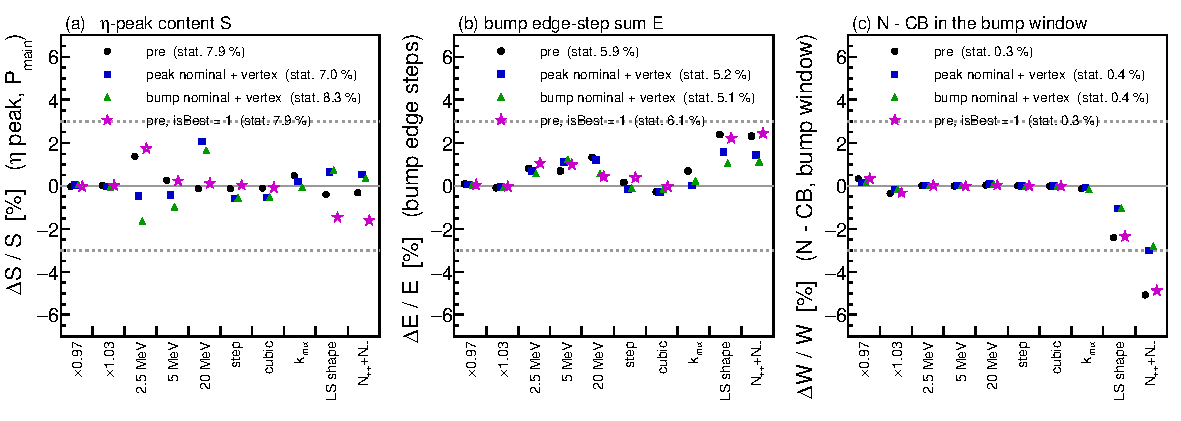
\includegraphics[width=\textwidth]{figs_exp/cb_sensitivity.pdf}
\caption{Relative change in per cent of (a) the $\eta$-peak content $S$ (\Pmain), (b) the bump edge-step sum $E$, (c)
$N-\mathrm{CB}$ in the bump window $W$, when the CB estimate is changed. Selection: data with the base cuts \ptthreecap{}, an event vertex reconstructed ($\vz>-500$\,mm) and inside the target region ($\vz>-160$\,mm), particles identified by the START-free velocity \betanew (pions within $3\sigma$, leptons within $5\sigma$ of the expected band; leptons with a RICH ring), energy-loss-corrected momenta for all four tracks, all stored \ppee combinations of each event (isBest $\ge0$) (together ``pre''); four selections: ``pre''; ``pre'' and angle between the \pipi and the \ee momenta in the laboratory $\alab<55^\circ$, $\Mpipi>0.30$\,\GeVcc and both pion tracks used in the fit of the event vertex (peak nominal + vertex); ``pre'' and $\alab<40^\circ$, $0.30<\Mpipi<0.41$\,\GeVcc and both pions in the vertex fit (bump nominal + vertex); ``pre'' with only the best-ranked combination of each event (isBest $=1$); $S$ from the fit in 0.5225--0.6100\,\GeVcc, $E$ from the four \Mpipi slices 0.30--0.34, 0.34--0.37, 0.37--0.39 and 0.39--0.40\,\GeVcc, $W$ in the data bump window $0.4550\le\Mfour<0.5225$\,\GeVcc. Data; ``pre'', peak nominal + vertex, bump
nominal + vertex (isBest $\ge0$) and ``pre'' with isBest $=1$; the legend gives the statistical error of each
quantity. Variants: CB$\times0.97$, $\times1.03$; CB bins of 2.5, 5, 20\,\MeVcc; step and cubic interpolation;
CB$\times k_{\mathrm{mix}}(\Mfour)$ (not for isBest $=1$); like-sign sum shape; plain $N_{++}+N_{--}$ (extreme). Dotted:
$\pm3$\,\%. Equal y ranges; not normalised to luminosity.}
\label{fig:cb_sensitivity}
\end{figure}

\subsection{The factor \texorpdfstring{$k$}{k} from event mixing}
\label{sec:kmix}
\textbf{Procedure} (as in the \ee channel study): $k(M)=N_{+-}^{\mathrm{mix}}/(2\sqrt{N_{++}^{\mathrm{mix}}N_{--}^{\mathrm{mix}}})$.
The pool contains every \ee event of ``pre'' (distinct tracks of the \code{cor_ok} counts, pion pairs as they occur
in the counts; a lepton is never combined with a pion pair that uses the same track). Variant A combines the pion pair
and \emph{one} lepton of the current event with the other lepton from one of the last 10 earlier events of the same
20\,mm vertex-$z$ class: $(\pi\pi e^+)_E e^-_B$ and $(\pi\pi e^-)_E e^+_B$ for $N_{+-}$, $(\pi\pi e^+)_E e^+_B$ for
$N_{++}$, $(\pi\pi e^-)_E e^-_B$ for $N_{--}$. All selection cuts are applied to the mixed combination (OA, \alab,
\MMfour recomputed; \Mpipi, the pion vertex flags and \dzpi from the event). Errors from 10 sub-samples;
3\,783\,447 events, $2.7\times10^8$ mixed combinations in 0.35--0.95\,\GeVcc. Variants: one pool for all $z$; events
with $\ge3$ leptons only; B, both leptons from two other events; C, lepton pairs alone ($k_{ee}$ against \Mee), carried
to \Mfour through the \Mee of the like-sign counts.

\textbf{Result} (Table~\ref{tab:cb_kmix}, Fig.~\ref{fig:cb_kmix}): for ``pre'' and the peak selections $k=0.976$--0.985
below the bump (PEAK 1.021), 1.011--1.023 in the bump window, 1.025--1.034 in 0.5225--0.56, 1.034--1.042 in 0.56--0.60 and
1.035--1.040 in 0.60--0.70\,\GeVcc; the three bump-nominal variants reach 1.033--1.034 in the bump window, 1.071--1.073 in
0.5225--0.56, 1.082--1.085 in 0.56--0.60 and 1.067--1.069 in 0.60--0.70. The pools differ by about $\pm0.005$ (bump)
and $\pm0.008$ (peak region); variant B equals A within 0.004 (the pion--lepton correlation does not matter), C agrees
in the bump window and is 0.011 lower in 0.5225--0.56: $k$ is mostly a property of the lepton pair. The channel's
$k_{ee}$ reproduces the structure of the \ee channel study within 0.002--0.012. The \emph{shape} of the mixed like-sign
combinations differs strongly from the real like-sign counts (ratio 4.5/3.0 at 0.35--0.40 to 0.73/0.76 at 0.90--0.95):
only the ratio $k$ is taken from mixing, never the shape. Applying $k_A(\Mfour)$ changes $S$ by $-0.07$ to $+0.57$\,\%,
$E$ by up to $+0.7$\,\% and $W$ by $-0.07$ to $-0.42$\,\%.

The $\pm3$\,\% band of the $k=1$ convention therefore covers the measured $k$ in the bump window for all selections
except the three bump-nominal variants (bump nominal, + vertex, + OA$>2^\circ$), lies at the edge in 0.5225--0.56 and does
not cover 0.56--0.70. Mixing cannot see correlated $e^-e^-$ sources (\S\ref{sec:cbshare}), so $k_{\mathrm{mix}}$ tests the
acceptance factorisation, not the normalisation of the CB. Because the polynomial absorbs a
smooth change, the effect on $S$ and $E$ stays below 0.6--0.7\,\%. The realistic uncertainty of $k$ is the pool
spread, about 0.01, plus the method itself.

% written by plots/exp_report/cb_kmix.C
\begin{table}[H]\centering\footnotesize\setlength{\tabcolsep}{3pt}
\caption{Event-mixing correction $k=N_{+-}^\text{mix}/(2\sqrt{N_{++}^\text{mix}N_{--}^\text{mix}})$ of the like-sign CB, experimental data, isBest $\geq 0$. Mixed combination: pion pair and one lepton of an event, the other lepton from one of the last 10 events of the same vertex-$z$ class (20~mm); the selection is applied to the mixed combination. Mean of $k$ weighted with the data CB of the selection in regions of $M(\pi^+\pi^-e^+e^-)$ [GeV/$c^2$]; errors from 10 sub-samples. Last columns: relative change of the $\eta$-peak content $S$ ($P_\text{main}$) and of $N-\text{CB}$ in the bump window ($W$) when the CB is multiplied by $k(M)$. Not normalised to luminosity.}
\label{tab:cb_kmix}
\resizebox{\textwidth}{!}{%
\begin{tabular}{lrrrrrrrr}
\toprule
selection & 0.35--0.455 & bump & 0.5225--0.56 & 0.56--0.60 & 0.60--0.70 & 0.70--0.95 & $\Delta S/S$ & $\Delta W/W$\\
\midrule
pre & $0.980\pm0.001$ & $1.013\pm0.001$ & $1.030\pm0.001$ & $1.037\pm0.001$ & $1.035\pm0.000$ & $1.022\pm0.000$ & +0.47\% & -0.14\%\\
pre + OA$>$2 & $0.981\pm0.001$ & $1.013\pm0.001$ & $1.030\pm0.001$ & $1.037\pm0.001$ & $1.035\pm0.000$ & $1.022\pm0.000$ & +0.57\% & -0.19\%\\
pre + vertex & $0.985\pm0.001$ & $1.013\pm0.001$ & $1.030\pm0.001$ & $1.039\pm0.001$ & $1.037\pm0.000$ & $1.023\pm0.000$ & +0.24\% & -0.08\%\\
DIRECT (pre+dz\_pi$<$40) & $0.981\pm0.001$ & $1.011\pm0.001$ & $1.029\pm0.001$ & $1.038\pm0.001$ & $1.037\pm0.000$ & $1.023\pm0.000$ & +0.29\% & -0.09\%\\
PEAK (DIRECT+MM4$<$2.85) & $1.021\pm0.002$ & $1.023\pm0.001$ & $1.025\pm0.001$ & $1.034\pm0.001$ & $1.036\pm0.000$ & $1.023\pm0.000$ & +0.28\% & -0.16\%\\
peak nominal & $0.976\pm0.001$ & $1.014\pm0.001$ & $1.033\pm0.001$ & $1.040\pm0.001$ & $1.038\pm0.000$ & $1.026\pm0.000$ & +0.44\% & -0.14\%\\
peak nominal + vertex & $0.981\pm0.002$ & $1.014\pm0.001$ & $1.033\pm0.001$ & $1.042\pm0.001$ & $1.040\pm0.001$ & $1.026\pm0.000$ & +0.22\% & -0.07\%\\
bump nominal & $0.986\pm0.001$ & $1.033\pm0.001$ & $1.071\pm0.001$ & $1.082\pm0.001$ & $1.067\pm0.001$ & $1.062\pm0.001$ & +0.11\% & -0.32\%\\
bump nominal + vertex & $0.990\pm0.002$ & $1.034\pm0.001$ & $1.073\pm0.001$ & $1.085\pm0.001$ & $1.069\pm0.001$ & $1.062\pm0.001$ & -0.07\% & -0.18\%\\
peak nominal + OA$>$2 & $0.977\pm0.001$ & $1.014\pm0.001$ & $1.034\pm0.001$ & $1.040\pm0.001$ & $1.038\pm0.000$ & $1.026\pm0.000$ & +0.54\% & -0.19\%\\
bump nominal + OA$>$2 & $0.986\pm0.001$ & $1.033\pm0.001$ & $1.071\pm0.001$ & $1.082\pm0.001$ & $1.067\pm0.001$ & $1.062\pm0.001$ & +0.16\% & -0.42\%\\
\bottomrule
\end{tabular}}
\end{table}


\begin{figure}[!htb]
\centering
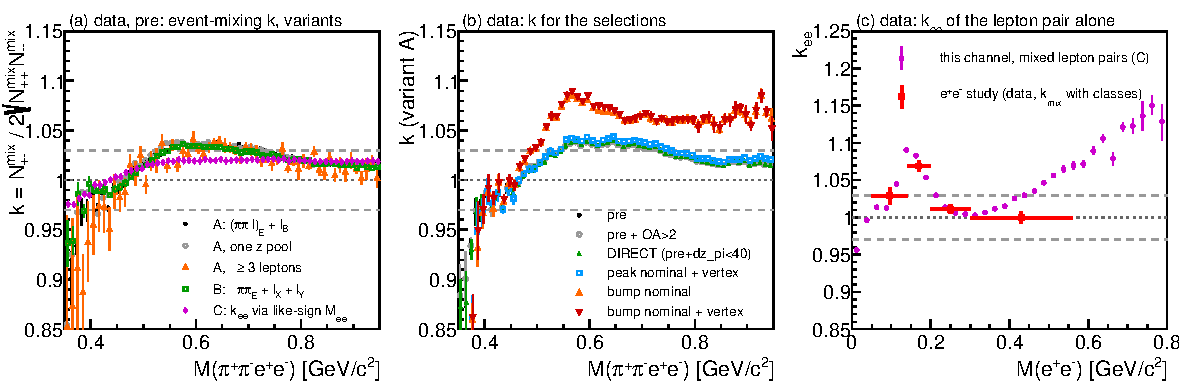
\includegraphics[width=\textwidth]{figs_exp/cb_kmix.pdf}
\caption{Event-mixing correction $k=N_{+-}^{\mathrm{mix}}/(2\sqrt{N_{++}^{\mathrm{mix}}N_{--}^{\mathrm{mix}}})$ of the
like-sign CB, data, isBest $\ge0$. Selection: data; event pool: every \ee event of ``pre'' (\ptthreecap{}, an event vertex reconstructed ($\vz>-500$\,mm) and inside the target region ($\vz>-160$\,mm), particles identified by the START-free velocity \betanew (pions within $3\sigma$, leptons within $5\sigma$ of the expected band; leptons with a RICH ring), energy-loss-corrected momenta for all four tracks, all stored \ppee combinations of each event (isBest $\ge0$)); all cuts of a selection act on the mixed combination; (a) ``pre''; (b) ``pre''; ``pre'' and \ee opening angle OA$>2^\circ$; ``pre'' and both pion tracks within 40\,mm of the event vertex along the beam ($\dzpi<40$\,mm) (DIRECT); ``pre'' and angle between the \pipi and the \ee momenta in the laboratory $\alab<55^\circ$, $\Mpipi>0.30$\,\GeVcc and both pion tracks used in the fit of the event vertex (peak nominal + vertex); ``pre'' and $\alab<40^\circ$, $0.30<\Mpipi<0.41$\,\GeVcc (bump nominal); bump nominal and both pions in the vertex fit (bump nominal + vertex); (c) lepton pairs of the ``pre'' events (magenta), and the values of the \ee channel study (red; data, PT3; quoted from that study, with its own selection). Variant A: pion pair and one lepton of an event plus the other lepton from one of
the last 10 events of the same 20\,mm $\vz$ class; all cuts act on the mixed combination; errors from 10
sub-samples; dashed: $k=0.97$ and 1.03. (a) ``pre'', variants A, one $\vz$ pool, $\ge3$ leptons, B (both leptons
foreign), C (lepton pairs alone, carried to \Mfour through \Mee). (b) Variant A for ``pre'', pre + OA$>2^\circ$, DIRECT,
peak nominal + vertex, bump nominal, bump nominal + vertex. (c) $k_{ee}$ against \Mee: this channel (magenta) and the
\ee channel study (red, data, PT3). $k$ is a ratio of mixed counts; no luminosity normalisation.}
\label{fig:cb_kmix}
\end{figure}

\notebox{\textbf{Combinatorial background, summary.} CB$/N$ in the peak window is 0.103 (``pre''), 0.076 (DIRECT),
0.072 (PEAK), 0.055 (peak nominal + vertex), 0.019 (X17 band): the CB is a small part of the background; the
physical background dominates. The like-sign spectra show no $\eta$ peak (pull $-0.43$) and no bump edge in \Mfour
($E_{\mathrm{ls}}=0.5\pm25.6$); in $u$ the $e^-e^-$ counts step by $73.5\pm15.7$ counts (4.7$\sigma$; 3\,\% of the bump step
through the CB): lepton pairs from the two \piz photons at large \Mee, subtracted with their \ee partners as designed (\S\ref{sec:cbnull}). $S$ and $E$ change by less than 0.1\,\% for CB$\pm3$\,\% and by less than 0.6--0.7\,\% for
$k_{\mathrm{mix}}=1.01$--1.04; window counts $W$ follow the CB directly. The normalisation of the CB cannot be checked with
data alone: $N_{--}/N_{++}=5.4$ against 1.17 for independent leptons (correlated $e^-e^-$ sources, which mixing cannot see),
like-sign pairs on one ring; the simulation does not reproduce the CB. Robust bound: the plain sum $N_{++}+N_{--}$ (CB
$+38$--45\,\%) changes $S$ by $\le1$\,\%, $E$ by $\le3$\,\% and $W$ by up to $-7$\,\%; CB$/N$ and $W$ carry an unknown scale.
Convention kept: $k=1$; ``CB$\times k_{\mathrm{mix}}$'' is quoted as a systematic variant.}

%======================================================================
\section{Optimisation of the selection}
\label{sec:opt}
%======================================================================

\inshort{The selection PEAK, frozen on the simulation, gains as much precision over ``pre'' as the best blind procedure on the data ($+1.35$ against $+1.36$ in $F$); the vertex cuts do most of the work and OA$>2^\circ$ never helps. Recommended: PEAK for the peak, BUMP $=$ ``pre'' for the bump, the frozen X17 cuts with the X17 window moved to the data mass scale (\S\ref{sec:recommend}).}

\subsection{Approach}
\label{sec:optapproach}
In the data the signal cannot be separated from the background combination by combination, so a cut can only be judged by
what it does to the fitted signal: the $\eta$-peak content $S$ and its statistical precision $F=S/\mathrm{stat}$,
the bump visibility $E$ and the tagged-$\eta$ content $T$. Two traps come with this. \textbf{Optimisation
bias}: choosing the cuts that maximise $F$ on the same data also selects upward fluctuations (\S\ref{sec:bias}).
\textbf{Sculpting}: a cut whose pass fraction changes with \Mfour inside the fit range can make a peak-like
structure out of a smooth background (\S\ref{sec:sculpt}). The study therefore (i) measures every cut by
pass/fail fits, (ii) flags sculpting cuts with mixed events, (iii) measures the bias of data-driven choices
on independent halves, and (iv) applies the selections frozen in the simulation study, which were chosen
without these data. All numbers in this section use ``pre'' as the base (the first study started without
$\vz>-160$\,mm; its numbers are quoted only where marked) and all combinations (isBest $\ge0$) unless stated;
isBest $=1$ and OA$>2^\circ$ are given as variants.

\subsection{Named selections on the data}
\label{sec:named}
Table~\ref{tab:opt_named} and Fig.~\ref{fig:opt_named_summary} compare the named selections;
Table~\ref{tab:opt_named_variants} gives the four variants (isBest $\ge0$ or $=1$, without or with OA$>2^\circ$);
Fig.~\ref{fig:opt_named_spectra} shows the peak of four of them and Fig.~\ref{fig:opt_named_tagged} the tagged $\eta$.
\begin{itemize}
\setlength{\itemsep}{0pt}
\item The vertex cuts raise $F$ from 12.74 (``pre'') to 13.74 (DIRECT), 14.09 (PEAK) and 14.31 (pre + vertex, peak
      nominal + vertex); the kinematic cuts alone give 13.23 (peak nominal).
\item \textbf{OA$>2^\circ$} keeps 0.78 of the peak and 0.75 of $E$ and lowers $F$ in every selection by 1.4--2.1 units
      (in the X17 band it changes nothing, the \Mee band already implies a large OA). It never helps.
\item \textbf{isBest $=1$} keeps 0.90--0.93 of $S$ at about the same $F$ (``pre'' 12.74/12.74, PEAK 14.09/14.44); with the
      event-group term in the errors of the main variant, $F_g$ (``pre'' 12.54, PEAK 13.94), isBest $=1$ is at least as
      precise: all combinations add about 10\,\% signal and no precision.
\item The \textbf{CB scale} ($\pm3$\,\%) changes $S$ by at most 3 counts (``pre'' 4669/4672, PEAK 4366/4363) and $E$ by at
      most 2 counts.
\item ``slides'' and ``old code'' contain $\aeta>140^\circ$, a band-pass in \Mfour: their summed edge fits fail
      ($\chi^2$ 631/120 and 805/120), so their $E$ is not valid, and the cut keeps only 0.55/0.72 of $T$.
\item The bump gains visibility through the cuts: $Q=E/\sqrt{N_b}$ is 3.06 (``pre''), 3.36 (DIRECT, PEAK, bump
      nominal) and 3.60 (bump nominal + vertex); gain$_T=1.20$ for bump nominal + vertex.
\item The ECAL-tagged $T$ of ``pre'' is $3312\pm105$ in this chapter's copy of the procedure and $3314\pm105$ in the
      results chapter (\S\ref{sec:tagged}); the difference of 2 counts is far below the error.
\end{itemize}

% opt_named_cnt.tex: copy of opt_named.tex with "rows" -> "counts" (analyst, 15 Nov 2026; Part II writer, integ4)
% opt_named.tex -- written by plots/exp_report/opt_named.C (numbers: tables_exp/opt_named.txt)
\begin{table}[H]
\centering\footnotesize
\setlength{\tabcolsep}{3pt}
\caption{Named selections on the data, all stored combinations (isBest $\geq 0$), no OA cut. pre = $v_z>-160$~mm, corrected momenta (cor\_ok $=1$), PT3, FAT vertex $z>-500$~mm. $\eta$ peak: $P_\mathrm{main}$ fit of $N-\mathrm{CB}$ (frozen Gaussian 0.5439~GeV/$c^2$, $\sigma=5.4$~MeV, pol2, 0.5225--0.6100), $S$ = whole Gaussian $\pm$ stat $\pm$ model spread (old envelope; revised model uncertainty in Table~\ref{tab:fix_spread}); stat and the $E$ errors are per-count Poisson fit errors (no event-group term; the halving test of Table~\ref{tab:fix_stat} finds those of $E$ too small by a factor 1.2); $N$, CB/$N$ and $S/B$ in the data window 0.53364--0.55416~GeV/$c^2$; $F=S/\sigma_S^\mathrm{stat}$ compares selections and is not a significance. Bump: edge-step visibility $E$ (counts per 2.5~MeV, not a yield) $\pm$ stat $\pm$ spread. $T$: ECAL-tagged $\eta\to\pi^+\pi^-\pi^0$ (verification only), $\varepsilon_T=T/T(\mathrm{pre})$. CB $=2\sqrt{N_{++}N_{--}}$, $k=1$. Frozen = chosen on the simulation alone (freeze rule declared before the search); these data were not used in the choice. $E$ in brackets with $^\dagger$: the summed edge fit fails ($p<10^{-3}$, the $\eta$-rest angle cut is a band-pass in $M_4$), $E$ is not valid. Counts, not normalised to luminosity.}
\label{tab:opt_named}
\begin{tabular}{lrrrrrrrr}
\toprule
Selection & $N$ & CB/$N$ & $S\pm$stat$\pm$spread & $S/B$ & $F$ & $E\pm$stat$\pm$spread & $T\pm$stat & $\varepsilon_T$ \\
\midrule
pre without $v_z>-160$ & 86011 & 0.134 & $4657\pm390\pm1233$ & 0.054 & 11.9 & $1241\pm76\pm319$ & $3300\pm108$ & 0.996 \\
\midrule
pre = BUMP (frozen) & 77513 & 0.103 & $4671\pm367\pm958$ & 0.060 & 12.7 & $1199\pm71\pm287$ & $3312\pm105$ & 1.000 \\
peak nominal & 61800 & 0.097 & $4330\pm327\pm981$ & 0.071 & 13.2 & $1169\pm68\pm301$ & $3184\pm98$ & 0.961 \\
peak nominal + vertex & 45433 & 0.055 & $3949\pm276\pm936$ & 0.089 & 14.3 & $1089\pm57\pm262$ & $2968\pm89$ & 0.896 \\
peak nominal + $\Delta z_\pi<40$ & 50604 & 0.071 & $4182\pm293\pm837$ & 0.084 & 14.3 & $1139\pm60\pm253$ & $3050\pm91$ & 0.921 \\
DIRECT (frozen) & 62969 & 0.076 & $4492\pm327\pm907$ & 0.072 & 13.7 & $1183\pm63\pm226$ & $3191\pm97$ & 0.963 \\
PEAK (frozen) & 56532 & 0.072 & $4364\pm310\pm867$ & 0.078 & 14.1 & $1120\pm59\pm243$ & $2972\pm92$ & 0.897 \\
pre + vertex & 55947 & 0.059 & $4388\pm307\pm1078$ & 0.080 & 14.3 & $1142\pm59\pm236$ & $3088\pm94$ & 0.932 \\
\midrule
bump nominal & 33240 & 0.099 & $2635\pm237\pm431$ & 0.081 & 11.1 & $1082\pm60\pm326$ & $3014\pm93$ & 0.910 \\
bump nominal + vertex & 24568 & 0.058 & $2405\pm200\pm456$ & 0.102 & 12.0 & $1004\pm51\pm244$ & $2820\pm84$ & 0.851 \\
bump nominal + $\Delta z_\pi<40$ & 27289 & 0.073 & $2600\pm212\pm477$ & 0.099 & 12.3 & $1040\pm54\pm265$ & $2895\pm87$ & 0.874 \\
\midrule
slides & 46001 & 0.122 & $3187\pm283\pm673$ & 0.070 & 11.2 & (918)$^\dagger$ & $1819\pm75$ & 0.549 \\
old code & 51605 & 0.097 & $3633\pm296\pm671$ & 0.071 & 12.3 & (1239)$^\dagger$ & $2391\pm85$ & 0.722 \\
\bottomrule
\end{tabular}
\end{table}


% opt_named_variants_cnt.tex: copy of opt_named_variants.tex with "rows" -> "counts" (analyst, 15 Nov 2026; Part II writer, integ4)
% opt_named_variants.tex -- written by plots/exp_report/opt_named.C (numbers: tables_exp/opt_named.txt)
\begin{table}[H]
\centering\footnotesize
\setlength{\tabcolsep}{3pt}
\caption{$\eta$ peak content $S\pm$stat$\pm$model spread (old envelope; revised: Table~\ref{tab:fix_spread}) and $F=S/\sigma_S^\mathrm{stat}$ of the named selections in the four variants: all stored combinations (isBest $\geq 0$, main) or isBest $=1$ (comparison), without and with OA$(e^+e^-)>2^\circ$ (OA $>2^\circ$ is not a fixed cut). Last column: edge-step visibility $E$ of the bump (isBest $\geq0$ / with OA $>2^\circ$); $^\dagger$: summed edge fit fails ($p<10^{-3}$), $E$ not valid. Same fit and conventions as Table~\ref{tab:opt_named}. Counts, not normalised to luminosity.}
\label{tab:opt_named_variants}
\resizebox{\textwidth}{!}{%
\begin{tabular}{lcccccc}
\toprule
 & \multicolumn{2}{c}{isBest $\geq 0$} & \multicolumn{2}{c}{isBest $=1$} & \\
Selection & no OA cut & OA $>2^\circ$ & no OA cut & OA $>2^\circ$ & $E$ / $E$(OA$>2^\circ$) \\
\midrule
pre without $v_z>-160$ & $4657\pm390\pm1233$ (11.9) & $3629\pm352\pm951$ (10.3) & $4167\pm349\pm860$ (11.9) & $3271\pm314\pm667$ (10.4) & 1241 / 944 \\
\midrule
pre = BUMP (frozen) & $4671\pm367\pm958$ (12.7) & $3632\pm328\pm752$ (11.1) & $4199\pm330\pm671$ (12.7) & $3286\pm294\pm555$ (11.2) & 1199 / 898 \\
peak nominal & $4330\pm327\pm981$ (13.2) & $3391\pm291\pm721$ (11.6) & $3895\pm295\pm776$ (13.2) & $3080\pm262\pm667$ (11.8) & 1169 / 874 \\
peak nominal + vertex & $3949\pm276\pm936$ (14.3) & $3076\pm242\pm715$ (12.7) & $3602\pm252\pm750$ (14.3) & $2843\pm221\pm571$ (12.9) & 1089 / 811 \\
peak nominal + $\Delta z_\pi<40$ & $4182\pm293\pm837$ (14.3) & $3250\pm258\pm717$ (12.6) & $3817\pm266\pm763$ (14.3) & $2998\pm234\pm565$ (12.8) & 1139 / 836 \\
DIRECT (frozen) & $4492\pm327\pm907$ (13.7) & $3460\pm290\pm841$ (11.9) & $4112\pm296\pm677$ (13.9) & $3185\pm263\pm735$ (12.1) & 1183 / 877 \\
PEAK (frozen) & $4364\pm310\pm867$ (14.1) & $3302\pm274\pm681$ (12.0) & $4061\pm281\pm782$ (14.4) & $3098\pm248\pm573$ (12.5) & 1120 / 827 \\
pre + vertex & $4388\pm307\pm1078$ (14.3) & $3407\pm271\pm834$ (12.6) & $3966\pm280\pm955$ (14.2) & $3107\pm247\pm733$ (12.6) & 1142 / 862 \\
\midrule
bump nominal & $2635\pm237\pm431$ (11.1) & $1967\pm206\pm369$ (9.5) & $2371\pm214\pm396$ (11.1) & $1771\pm186\pm352$ (9.5) & 1082 / 812 \\
bump nominal + vertex & $2405\pm200\pm456$ (12.0) & $1745\pm172\pm335$ (10.1) & $2236\pm184\pm428$ (12.2) & $1627\pm158\pm300$ (10.3) & 1004 / 746 \\
bump nominal + $\Delta z_\pi<40$ & $2600\pm212\pm477$ (12.3) & $1943\pm183\pm331$ (10.6) & $2351\pm193\pm445$ (12.2) & $1752\pm167\pm292$ (10.5) & 1040 / 768 \\
\midrule
slides & $3187\pm283\pm673$ (11.2) & $3187\pm283\pm673$ (11.2) & $2933\pm255\pm580$ (11.5) & $2933\pm255\pm580$ (11.5) & (918)$^\dagger$ / (918)$^\dagger$ \\
old code & $3633\pm296\pm671$ (12.3) & $2830\pm261\pm494$ (10.9) & $3254\pm267\pm594$ (12.2) & $2544\pm235\pm465$ (10.8) & (1239)$^\dagger$ / (918)$^\dagger$ \\
\midrule
X17 band (frozen) & $440\pm92\pm133$ (4.8) & $441\pm92\pm136$ (4.8) & $368\pm84\pm122$ (4.4) & $372\pm84\pm123$ (4.4) & 110 / 110 \\
\bottomrule
\end{tabular}}
\end{table}


\begin{figure}[H]
\centering
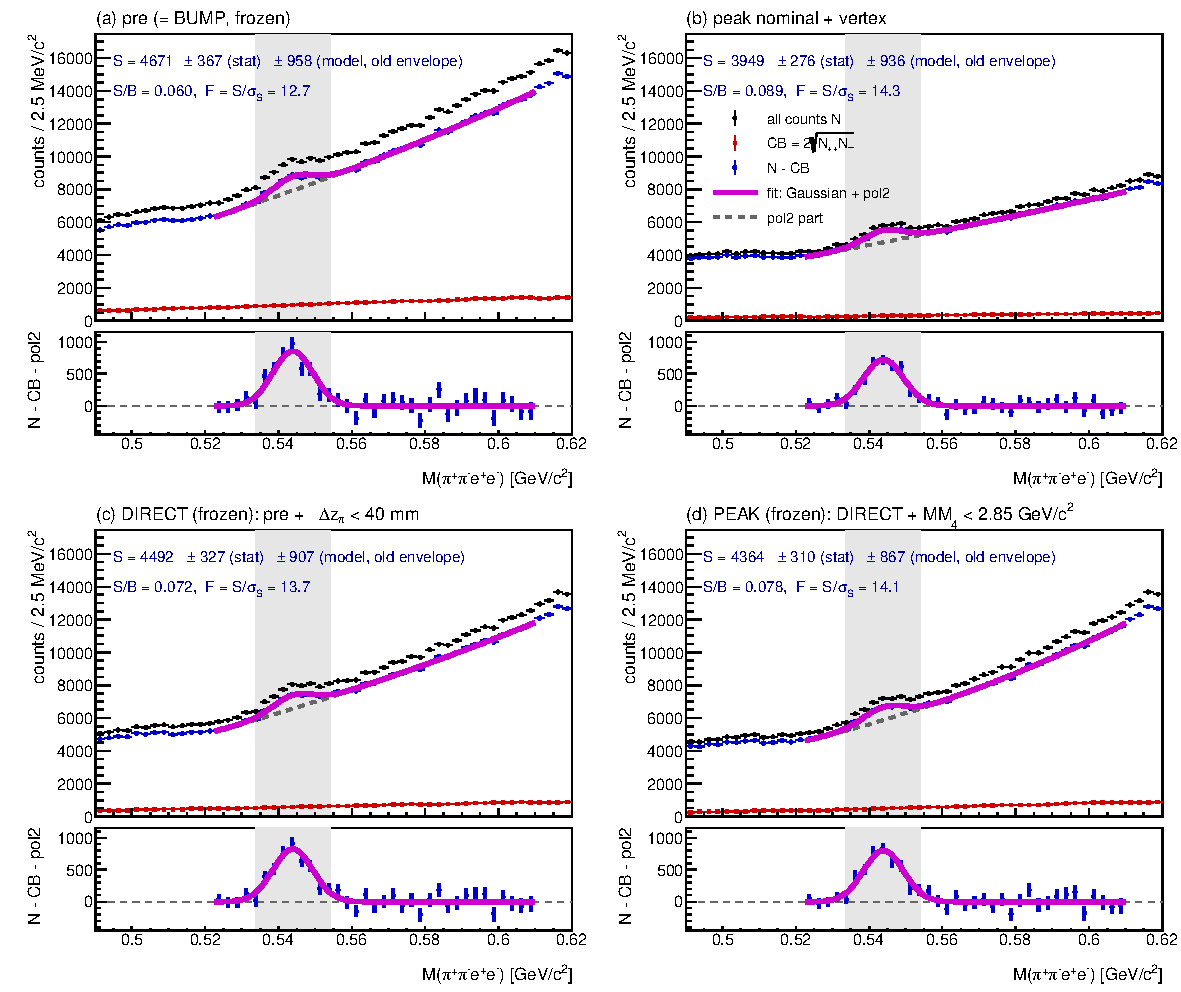
\includegraphics[width=\textwidth]{figs_exp/opt_named_spectra_cnt.pdf}
\caption{\Mfour of the data for (a) ``pre'' ($=$ BUMP), (b) peak nominal + vertex (data-optimised), (c) DIRECT (pre +
$\dzpi<40$\,mm), (d) PEAK (DIRECT + $\MMfour<2.85$\,\GeVcc); all combinations (isBest $\ge0$), corrected momenta, PT3,
$\vz>-500$\,mm, $\vz>-160$\,mm. Selection: data with the base cuts \ptthreecap{}, an event vertex reconstructed ($\vz>-500$\,mm) and inside the target region ($\vz>-160$\,mm), particles identified by the START-free velocity \betanew (pions within $3\sigma$, leptons within $5\sigma$ of the expected band; leptons with a RICH ring), energy-loss-corrected momenta for all four tracks, all stored \ppee combinations of each event (isBest $\ge0$) (together ``pre''); in addition (a) nothing, (b) angle between the \pipi and the \ee momenta in the laboratory $\alab<55^\circ$, $\Mpipi>0.30$\,\GeVcc and both pion tracks used in the fit of the event vertex, (c) both pion tracks within 40\,mm of the event vertex along the beam ($\dzpi<40$\,mm), (d) $\dzpi<40$\,mm and missing mass of \ppee below 2.85\,\GeVcc ($\MMfour<2.85$\,\GeVcc); the like-sign counts of the CB pass the same cuts. Top: $N$ (black), CB $=2\sqrt{N_{++}N_{--}}$ (red, $k=1$), $N-\mathrm{CB}$ (blue), \Pmain fit
(magenta; pol2 part grey dashed) in 0.5225--0.6100. Bottom: $N-\mathrm{CB}-\mathrm{pol2}$ with the Gaussian. Grey: data peak window.
$S\pm$stat$\pm$model spread (old envelope; revised values in Table~\ref{tab:fix_spread}), $S/B$, $F$ (statistical only). Equal y ranges; counts, not normalised to luminosity.}
\label{fig:opt_named_spectra}
\end{figure}

\begin{figure}[H]
\centering
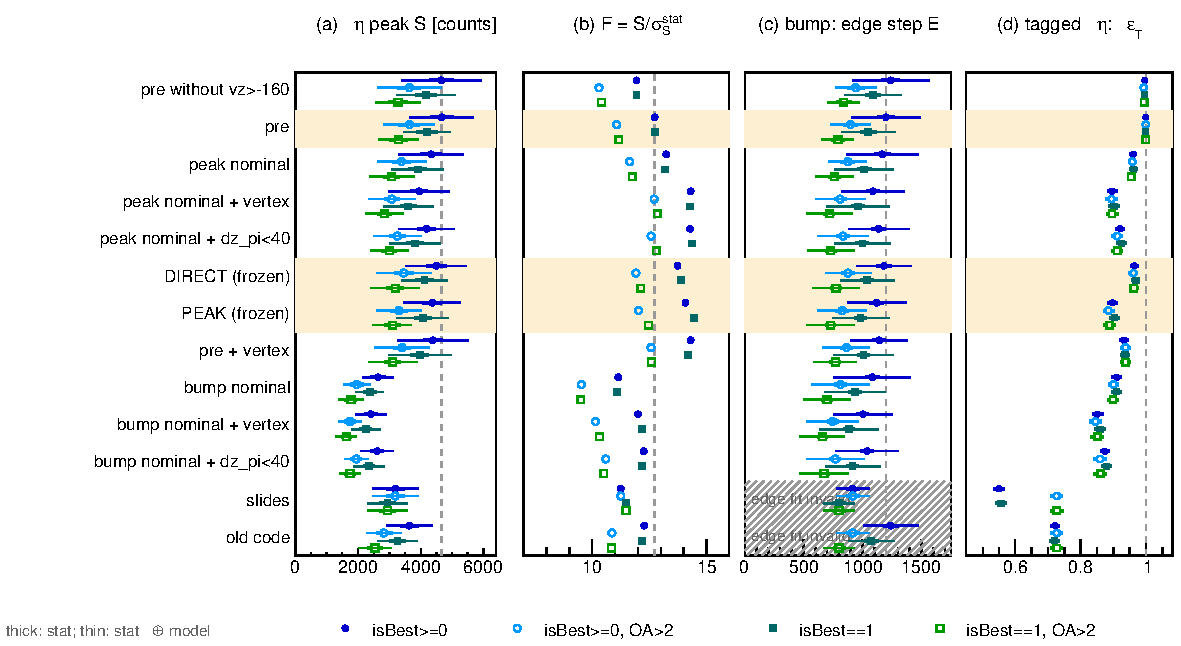
\includegraphics[width=\textwidth]{figs_exp/opt_named_summary_cnt.pdf}
\caption{Named selections on the data: (a) $\eta$-peak content $S$ (thick: stat; thin: stat $\oplus$ model spread, old envelope),
(b) $F=S/\sigma_S^{\mathrm{stat}}$, (c) edge-step visibility $E$ of the bump (counts per 2.5\,\MeVcc; not a yield), (d)
tagged-$\eta$ efficiency $\varepsilon_T$ relative to ``pre''. Selection: data with the base cuts \ptthreecap{}, an event vertex reconstructed ($\vz>-500$\,mm) and inside the target region ($\vz>-160$\,mm), particles identified by the START-free velocity \betanew (pions within $3\sigma$, leptons within $5\sigma$ of the expected band; leptons with a RICH ring), energy-loss-corrected momenta for all four tracks, all stored \ppee combinations of each event (isBest $\ge0$) (together ``pre''), thirteen selections: ``pre'' without its cut $\vz>-160$\,mm; ``pre'' ($=$ BUMP); peak nominal (``pre'' and angle between the \pipi and the \ee momenta in the laboratory $\alab<55^\circ$, $\Mpipi>0.30$\,\GeVcc); peak nominal + vertex (and both pion tracks used in the fit of the event vertex); peak nominal and $\dzpi<40$\,mm; DIRECT (``pre'' and both pion tracks within 40\,mm of the event vertex along the beam ($\dzpi<40$\,mm)); PEAK (DIRECT and $\MMfour<2.85$\,\GeVcc); pre + vertex; bump nominal (``pre'' and $\alab<40^\circ$, $0.30<\Mpipi<0.41$\,\GeVcc); bump nominal + vertex; bump nominal and $\dzpi<40$\,mm; slides (``pre'' and $\alab<50^\circ$, $\Mpipi<0.46$\,\GeVcc, $\eta$-rest angle $\aeta>140^\circ$, \ee opening angle OA$>2^\circ$); old code (``pre'' and $\alab<50^\circ$, $\Mpipi<0.42$\,\GeVcc, $\aeta>140^\circ$); each with all stored combinations (isBest $\ge0$) or only the best-ranked one (isBest $=1$), without or with OA$>2^\circ$; (c) $E$ from the four \Mpipi slices 0.30--0.34, 0.34--0.37, 0.37--0.39 and 0.39--0.40\,\GeVcc; (d) counts with an ECAL photon identified as a photon with $0.8<\beta<1.2$ and energy above 100\,MeV (of up to three such photons the one with $M(\ee\gamma)$ closest to 0.140\,\GeVcc), $0.119\le M(\ee\gamma)<0.173$\,\GeVcc and $\Mee<0.10$\,\GeVcc. Four variants: isBest $\ge0$ (main, blue full circles), isBest $\ge0$ with
OA$>2^\circ$ (light blue open circles), isBest $=1$ (dark cyan full squares), isBest $=1$ with OA$>2^\circ$ (green open squares). Shaded: selections frozen on simulation. Hatched in (c): the
summed edge fit fails ($p<10^{-3}$; slides, old code), $E$ not valid. Dashed: the value of ``pre''. Counts, not
normalised to luminosity.}
\label{fig:opt_named_summary}
\end{figure}

\begin{figure}[H]
\centering
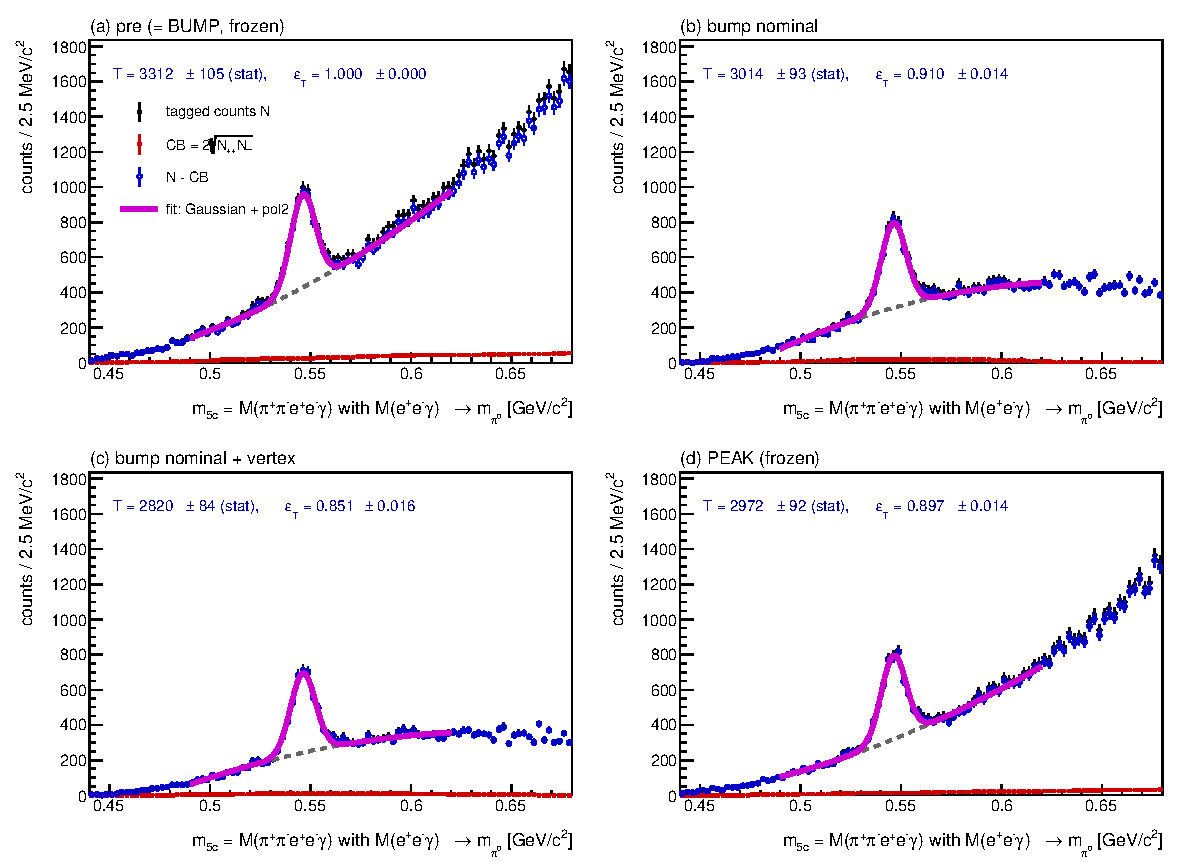
\includegraphics[width=\textwidth]{figs_exp/opt_named_tagged_cnt.pdf}
\caption{ECAL-tagged $\eta\to\pipi\piz$ (one good photon, $0.119\le M(\ee\gamma)<0.173$\,\GeVcc, $\Mee<0.1$\,\GeVcc):
$m_{5c}$ for (a) ``pre'', (b) bump nominal, (c) bump nominal + vertex, (d) PEAK; all combinations (isBest $\ge0$). Selection: data with the base cuts \ptthreecap{}, an event vertex reconstructed ($\vz>-500$\,mm) and inside the target region ($\vz>-160$\,mm), particles identified by the START-free velocity \betanew (pions within $3\sigma$, leptons within $5\sigma$ of the expected band; leptons with a RICH ring), energy-loss-corrected momenta for all four tracks, all stored \ppee combinations of each event (isBest $\ge0$) (together ``pre''); in addition (a) nothing, (b) angle between the \pipi and the \ee momenta in the laboratory $\alab<40^\circ$ and $0.30<\Mpipi<0.41$\,\GeVcc, (c) the same and both pion tracks used in the fit of the event vertex, (d) both pion tracks within 40\,mm of the event vertex along the beam ($\dzpi<40$\,mm) and $\MMfour<2.85$\,\GeVcc; in every panel an ECAL photon identified as a photon with $0.8<\beta<1.2$ and energy above 100\,MeV (of up to three such photons the one with $M(\ee\gamma)$ closest to 0.140\,\GeVcc), $0.119\le M(\ee\gamma)<0.173$\,\GeVcc and $\Mee<0.10$\,\GeVcc; $m_{5c}$ with the photon energy rescaled so that $M(\ee\gamma)=m_{\pi^0}$.
$N$ black, CB red, $N-\mathrm{CB}$ blue (open), fit (magenta) Gaussian 0.5463\,\GeVcc / 6.2\,\MeVcc + pol2 (grey dashed) in 0.49--0.62. $T$ = Gaussian
content, $\varepsilon_T=T/T(\mathrm{pre})$. ECAL used as an independent check only. Equal y ranges; counts, not normalised
to luminosity.}
\label{fig:opt_named_tagged}
\end{figure}

\subsection{\texorpdfstring{Single-cut and N$-$1 scans}{Single-cut and N-1 scans}}
\label{sec:scans}
Every cut was scanned alone from ``pre'' with pass and fail fits (Figs.~\ref{fig:opt_peak_single},
\ref{fig:opt_peak_eff}, \ref{fig:opt_bump_single}) and varied around the data-optimised selections with the other
cuts fixed (N$-$1, Figs.~\ref{fig:opt_peak_nm1}, \ref{fig:opt_bump_nm1}). For the peak ($F(\mathrm{pre})=12.74$):
\begin{itemize}
\setlength{\itemsep}{0pt}
\item OA lower cuts all lose (OA$>2^\circ$: $F=11.07$); OA upper cuts give no gain (best 12.86 at
      $20^\circ$).
\item \alab: plateau from $35^\circ$ to no cut, best $F=13.34$ at $50^\circ$, 13.18 at $55^\circ$
      ($\varepsilon_S=0.944\pm0.029$ against $\sqrt{\varepsilon_B}=0.918$).
\item $\Mpipi>0.30$: $F=13.10$ ($\varepsilon_S=0.987\pm0.022$), flat up to 0.34; upper \Mpipi cuts 0.39--0.50 all sculpt
      and all lose ($F$ 9.6--12.2).
\item $\MMfour$ upper cuts 2.60--2.90 are all flagged; $F$ reaches 13.75 at 2.80 and 13.01 at 2.85.
\item $\aeta>100$--$140^\circ$ is flat ($F$ 12.69--12.73); 150 and $160^\circ$ are flagged (band-pass; $\chi^2$ 159/31 at 160).
\item \dzpi and the vertex flag: \S\ref{sec:vertex}.
\end{itemize}
N$-$1 around peak nominal + vertex ($F=14.31$): removing $\alab<55^\circ$ gives 14.62, removing $\Mpipi>0.30$ gives
14.25; adding $\dzpi<30$\,mm 14.57, $\vz>-150$\,mm 14.59, OA$>2^\circ$ 12.70. \textbf{Once the vertex cut is in, the
kinematic cuts no longer improve $F$}: pre + vertex has the same $F=14.31$.

For the bump (gain$_T$ from the tagged $\eta$, gain$_E$ from the edge step): $\alab<30$--$40^\circ$ 1.07--1.08 /
1.00--1.04; $\Mpipi>0.30$ 1.031 / 1.065; $\Mpipi<0.40$--0.41 1.007--1.013; both pions in the vertex fit
$1.094\pm0.015$ / $1.118\pm0.037$; $\dzpi<40$\,mm $1.069\pm0.013$ / $1.096\pm0.030$; $\vz>-160$\,mm (from no $\vz$ cut)
1.060 ($-150$: 1.094); $\MMfour<2.85$ 0.987; OA lower cuts all lose (OA$>2^\circ$: 0.85); $\aeta>140^\circ$ makes the edge
fit invalid ($\chi^2$ 793/120, gain$_T$ 0.76). N$-$1 around bump nominal + vertex: gain$_T$ 1.044 ($\alab$), 1.011
($\Mpipi>0.30$), 1.020 ($\Mpipi<0.41$), 1.082 (both pions), 0.862 (OA$>2^\circ$).

\begin{figure}[!htbp]
\centering
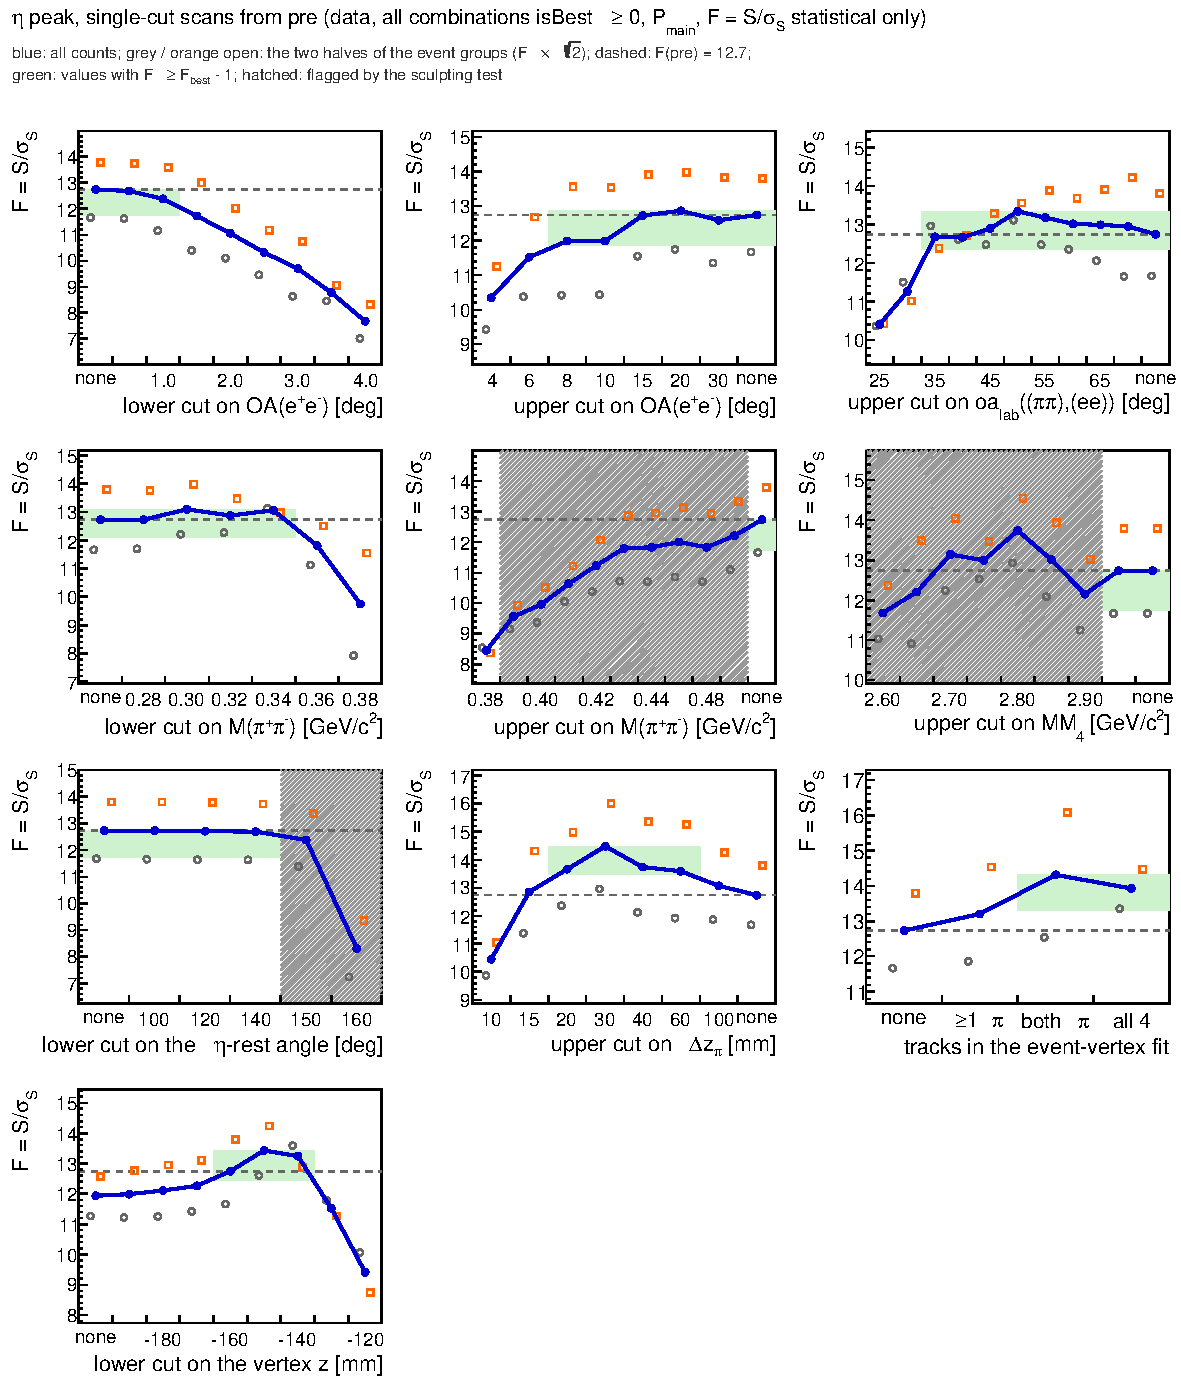
\includegraphics[width=0.93\textwidth]{figs_exp/opt_peak_single_cnt.pdf}
\caption{$\eta$ peak, single-cut scans from ``pre'' (data, isBest $\ge0$): $F=S/\sigma_S$ of \Pmain against the cut value
(blue); open grey/orange: the two halves of the event groups ($F\times\sqrt2$). Selection: data with the base cuts \ptthreecap{}, an event vertex reconstructed ($\vz>-500$\,mm) and inside the target region ($\vz>-160$\,mm), particles identified by the START-free velocity \betanew (pions within $3\sigma$, leptons within $5\sigma$ of the expected band; leptons with a RICH ring), energy-loss-corrected momenta for all four tracks, all stored \ppee combinations of each event (isBest $\ge0$) (together ``pre''), plus one cut at a time at the values on the horizontal axes (``none'': no cut): lower and upper cut on the \ee opening angle OA, upper cut on the angle \alab between the \pipi and the \ee momenta in the laboratory, lower and upper cut on \Mpipi, upper cut on \MMfour, lower cut on the $\eta$-rest angle \aeta, upper cut on \dzpi, the tracks required in the event-vertex fit, and a lower cut on \vz (this scan from ``pre'' without its cut $\vz>-160$\,mm); fits in 0.5225--0.6100\,\GeVcc. Dashed: $F(\mathrm{pre})$. Green:
values with $F\ge F_{\mathrm{best}}-1$. Hatched: values flagged by the sculpting test (\S\ref{sec:sculpt}). The $\vz$
threshold is scanned from ``pre'' without the $\vz$ cut. Counts, not normalised to luminosity.}
\label{fig:opt_peak_single}
\end{figure}

\begin{figure}[!htbp]
\centering
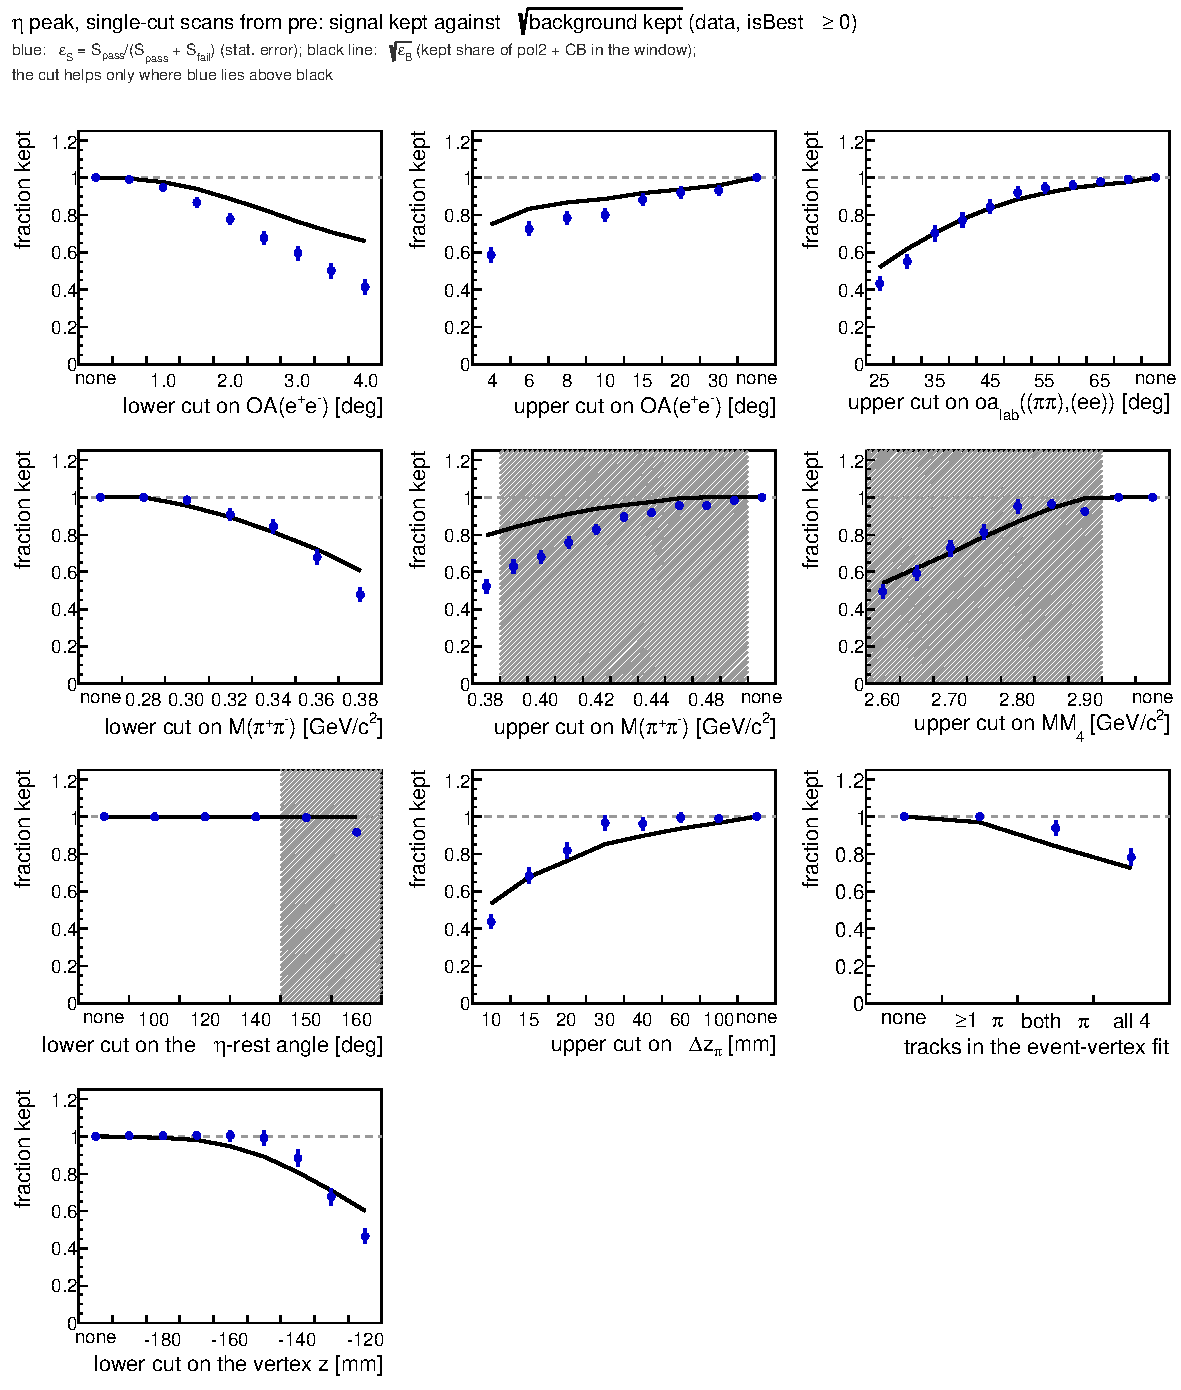
\includegraphics[width=0.93\textwidth]{figs_exp/opt_peak_single_eff.pdf}
\caption{The scans of Fig.~\ref{fig:opt_peak_single}: signal kept $\varepsilon_S=S_{\mathrm{pass}}/(S_{\mathrm{pass}}+S_{\mathrm{fail}})$
from fits of the passing and failing counts (blue, stat.\ errors) against $\sqrt{\varepsilon_B}$, the kept share of pol2 + CB
in the peak window (black line). Selection: as in Fig.~\ref{fig:opt_peak_single}: data with the base cuts \ptthreecap{}, an event vertex reconstructed ($\vz>-500$\,mm) and inside the target region ($\vz>-160$\,mm), particles identified by the START-free velocity \betanew (pions within $3\sigma$, leptons within $5\sigma$ of the expected band; leptons with a RICH ring), energy-loss-corrected momenta for all four tracks, all stored \ppee combinations of each event (isBest $\ge0$) (together ``pre''), plus one cut at a time at the values on the horizontal axes (the \vz scan from ``pre'' without its cut $\vz>-160$\,mm); $\varepsilon_B$ in the data peak window $0.53364\le\Mfour<0.55416$\,\GeVcc. A cut improves the statistical precision only where $\varepsilon_S>\sqrt{\varepsilon_B}$.
Data, isBest $\ge0$, base ``pre''.}
\label{fig:opt_peak_eff}
\end{figure}

\begin{figure}[!htbp]
\centering
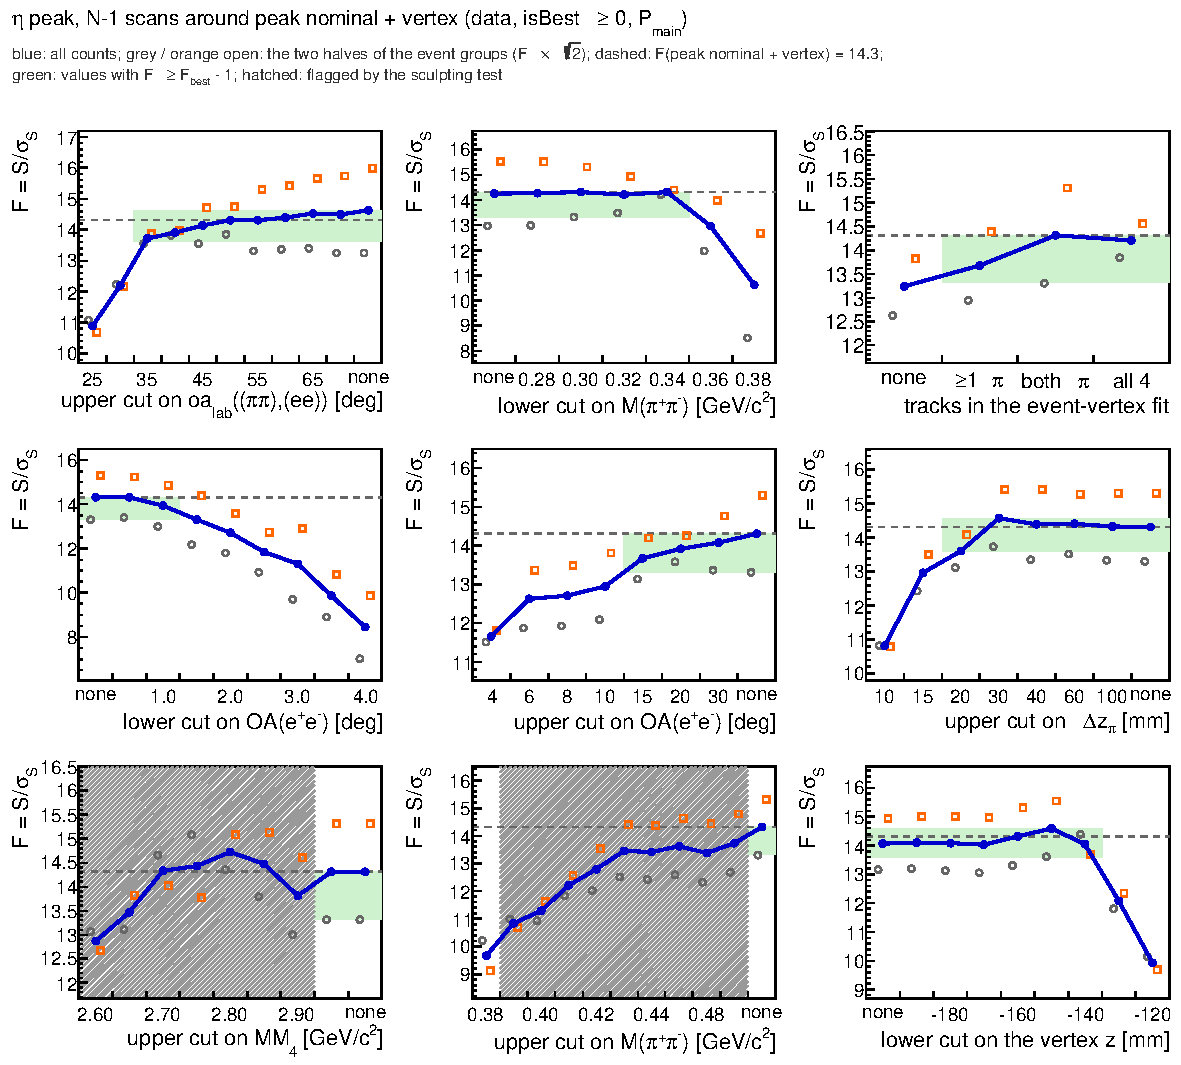
\includegraphics[width=0.93\textwidth]{figs_exp/opt_peak_nm1_cnt.pdf}
\caption{$\eta$ peak, N$-$1 scans around peak nominal + vertex ($\alab<55^\circ$, $\Mpipi>0.30$\,\GeVcc, both pions in the
vertex fit, on ``pre''): each cut varied with the others fixed. Selection: data with the base cuts \ptthreecap{}, an event vertex reconstructed ($\vz>-500$\,mm) and inside the target region ($\vz>-160$\,mm), particles identified by the START-free velocity \betanew (pions within $3\sigma$, leptons within $5\sigma$ of the expected band; leptons with a RICH ring), energy-loss-corrected momenta for all four tracks, all stored \ppee combinations of each event (isBest $\ge0$) (together ``pre''), angle between the \pipi and the \ee momenta in the laboratory $\alab<55^\circ$, $\Mpipi>0.30$\,\GeVcc and both pion tracks used in the fit of the event vertex (peak nominal + vertex); in each panel one of these three cuts is varied, or one cut is added (lower or upper OA cut, \dzpi, \MMfour, upper \Mpipi cut), or the \vz cut is moved, at the values on the horizontal axis, with the other cuts kept. Data, isBest $\ge0$. Symbols as in
Fig.~\ref{fig:opt_peak_single}.}
\label{fig:opt_peak_nm1}
\end{figure}

\begin{figure}[!htbp]
\centering
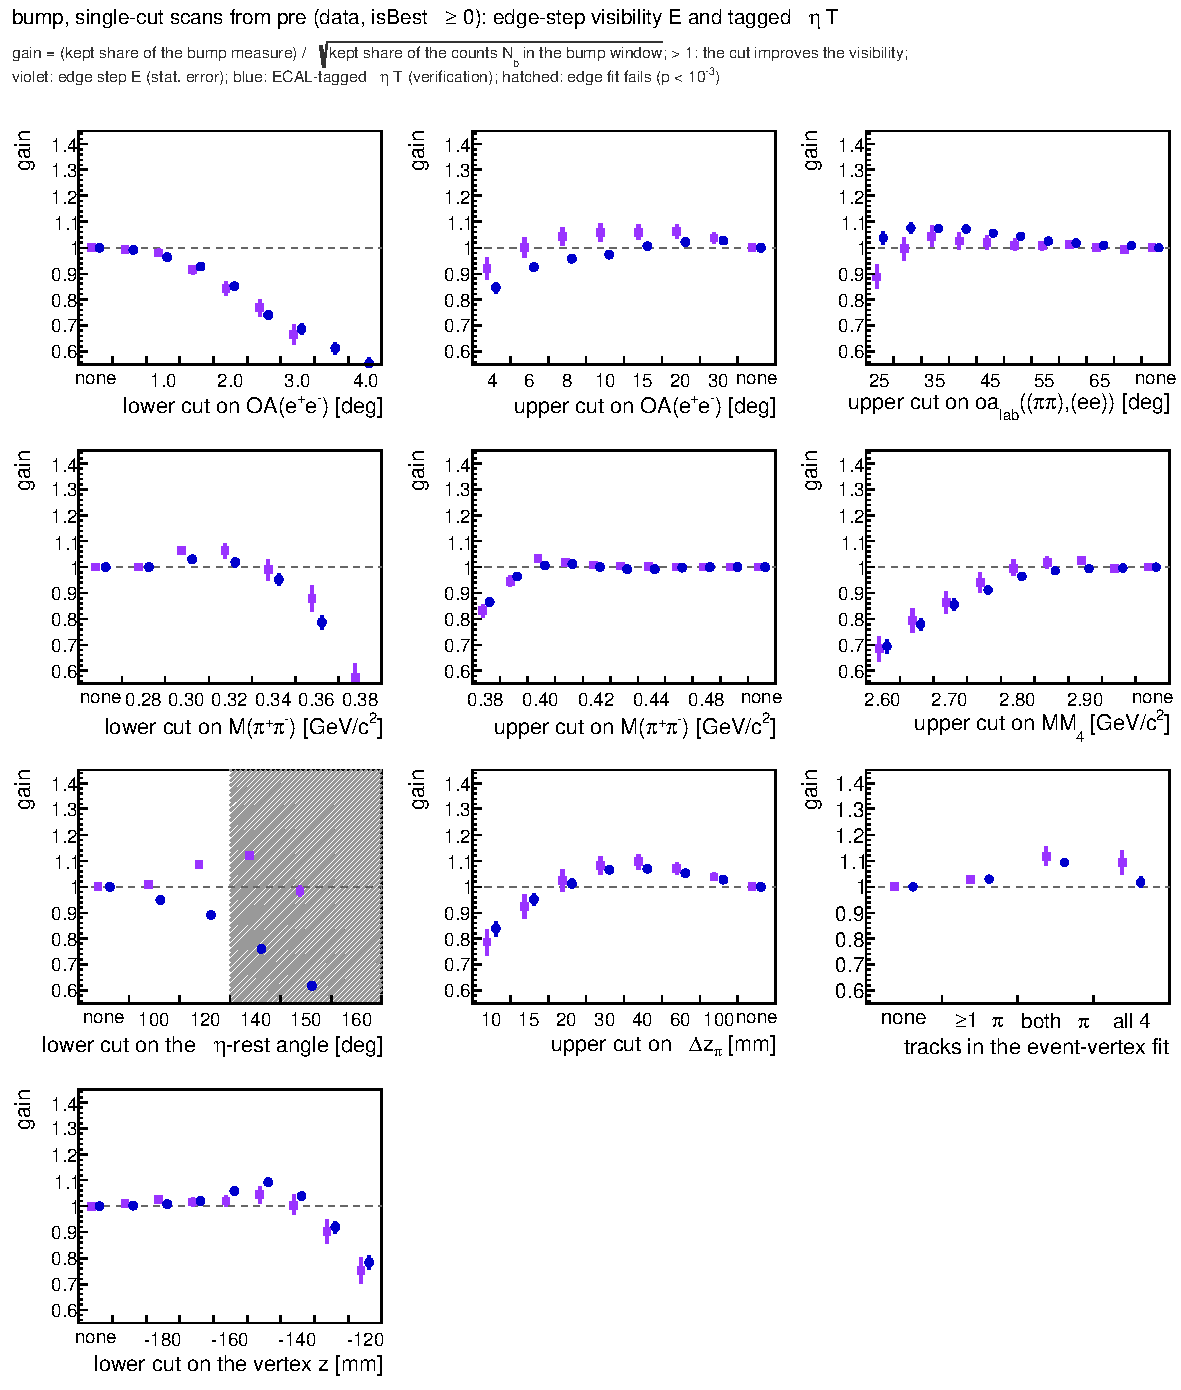
\includegraphics[width=0.93\textwidth]{figs_exp/opt_bump_single_cnt.pdf}
\caption{Bump, single-cut scans from ``pre'' (data, isBest $\ge0$): gain $=$ (kept share of the bump measure)$/\sqrt{\text{kept
share of the counts in the bump window 0.4550--0.5225}}$; violet: edge step $E$; blue: ECAL-tagged $\eta$ $T$. Selection: data with the base cuts \ptthreecap{}, an event vertex reconstructed ($\vz>-500$\,mm) and inside the target region ($\vz>-160$\,mm), particles identified by the START-free velocity \betanew (pions within $3\sigma$, leptons within $5\sigma$ of the expected band; leptons with a RICH ring), energy-loss-corrected momenta for all four tracks, all stored \ppee combinations of each event (isBest $\ge0$) (together ``pre''), plus one cut at a time at the values on the horizontal axes (the same cuts as in Fig.~\ref{fig:opt_peak_single}; the \vz scan from ``pre'' without its cut $\vz>-160$\,mm); $E$ from the four \Mpipi slices 0.30--0.34, 0.34--0.37, 0.37--0.39 and 0.39--0.40\,\GeVcc; $T$ from the counts with an ECAL photon identified as a photon with $0.8<\beta<1.2$ and energy above 100\,MeV (of up to three such photons the one with $M(\ee\gamma)$ closest to 0.140\,\GeVcc), $0.119\le M(\ee\gamma)<0.173$\,\GeVcc and $\Mee<0.10$\,\GeVcc; counts in the data bump window $0.4550\le\Mfour<0.5225$\,\GeVcc. Above 1 the cut
improves the visibility. Hatched: the summed edge fit fails ($p<10^{-3}$, band-pass cuts). Counts, not normalised to
luminosity.}
\label{fig:opt_bump_single}
\end{figure}

\begin{figure}[!htbp]
\centering
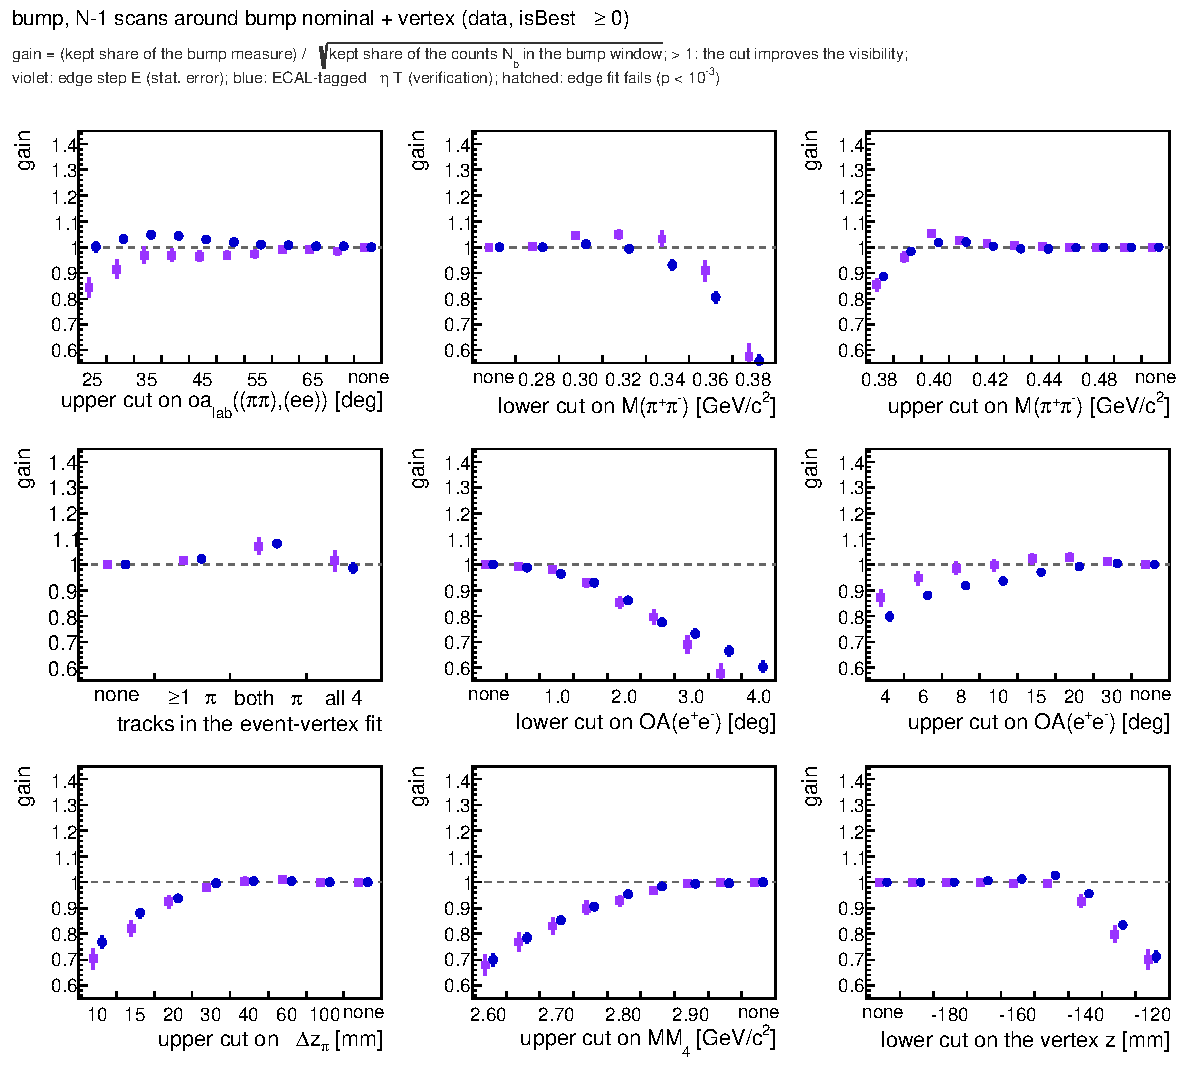
\includegraphics[width=0.93\textwidth]{figs_exp/opt_bump_nm1_cnt.pdf}
\caption{Bump, N$-$1 scans around bump nominal + vertex ($\alab<40^\circ$, $0.30<\Mpipi<0.41$\,\GeVcc, both pions in the
vertex fit, on ``pre''); data, isBest $\ge0$; symbols as in Fig.~\ref{fig:opt_bump_single}. Selection: data with the base cuts \ptthreecap{}, an event vertex reconstructed ($\vz>-500$\,mm) and inside the target region ($\vz>-160$\,mm), particles identified by the START-free velocity \betanew (pions within $3\sigma$, leptons within $5\sigma$ of the expected band; leptons with a RICH ring), energy-loss-corrected momenta for all four tracks, all stored \ppee combinations of each event (isBest $\ge0$) (together ``pre''), angle between the \pipi and the \ee momenta in the laboratory $\alab<40^\circ$, $0.30<\Mpipi<0.41$\,\GeVcc and both pion tracks used in the fit of the event vertex (bump nominal + vertex); in each panel one of these cuts is varied, or one cut is added (lower or upper OA cut, \dzpi, \MMfour), or the \vz cut is moved, at the values on the horizontal axis, with the other cuts kept; $E$, $T$ and the bump-window counts as in Fig.~\ref{fig:opt_bump_single}.}
\label{fig:opt_bump_nm1}
\end{figure}

\subsection{Cut flows}
\label{sec:optflow}
Table~\ref{tab:opt_cutflow} and Fig.~\ref{fig:opt_cutflow} build the three selections step by step. Along the
data-optimised peak selection $F$ goes 11.93 (no $\vz$ cut) $\to$ 12.74 ($\vz>-160$\,mm) $\to$ 13.18 ($\alab<55^\circ$) $\to$
13.23 ($\Mpipi>0.30$) $\to$ 14.31 (both pions in the vertex fit); the band of the $\vz$ step ($-170$/$-150$\,mm) is
12.27--13.43, that of the vertex step ($\ge1$ pion / all four tracks) 13.68--14.21. Along the bump selection $E$ falls
from 1241 to 1004 while $N_b$ falls from 170\,751 to 77\,735 counts (gain$_E$ 1.18, gain$_T$ 1.20, both relative to ``pre'';
relative to the start point without $\vz$ cut they would be 1.20 and 1.27). Along the frozen
selections $F$ goes $12.74\to13.74\to14.09$ with $S$ $4671\to4492\to4364$ and $E$ $1199\to1183\to1120$.

% opt_cutflow_cnt.tex: copy of opt_cutflow.tex with "rows" -> "counts" (analyst, 15 Nov 2026; Part II writer, integ4)
% opt_cutflow.tex -- written by plots/exp_report/opt_scans.C (numbers: tables_exp/opt_scans.txt)
\begin{table}[H]
\centering\footnotesize
\setlength{\tabcolsep}{3pt}
\caption{Cut flows on the data, all stored combinations (isBest $\geq 0$), corrected momenta, PT3, FAT vertex $z>-500$~mm; cuts added from top to bottom inside each block, rows marked ``no'' are not applied (each added to the last applied step). $N$, CB in the data peak window 0.53364--0.55416~GeV/$c^2$; $S\pm$stat$\pm$model spread from $P_\mathrm{main}$; $F=S/\sigma_S^\mathrm{stat}$; $E\pm$stat$\pm$spread = edge-step visibility of the bump (not a yield); $T$ = ECAL-tagged $\eta$. CB $=2\sqrt{N_{++}N_{--}}$, $k=1$. Counts, not normalised to luminosity.}
\label{tab:opt_cutflow}
\begin{tabular}{llrrrrrrr}
\toprule
Step & applied & $N$ & CB & $S\pm$stat$\pm$spread & $S/B$ & $F$ & $E\pm$stat$\pm$spread & $T\pm$stat \\
\midrule
\multicolumn{9}{l}{\textbf{$\eta$ peak, data-optimised}} \\
pre without vz cut & yes & 86011 & 11488 & $4657\pm390\pm1233$ & 0.054 & 11.9 & $1241\pm76\pm319$ & $3300\pm108$ \\
vz > -160 mm & yes & 77513 & 7949 & $4671\pm367\pm958$ & 0.060 & 12.7 & $1199\pm71\pm287$ & $3312\pm105$ \\
$\alpha_\mathrm{lab}$ < 55$^\circ$ & yes & 65749 & 6408 & $4444\pm337\pm1031$ & 0.068 & 13.2 & $1169\pm68\pm301$ & $3285\pm103$ \\
M($\pi\pi$) > 0.30 & yes & 61800 & 5996 & $4330\pm327\pm981$ & 0.071 & 13.2 & $1169\pm68\pm301$ & $3184\pm98$ \\
both $\pi$ in vertex fit & yes & 45433 & 2510 & $3949\pm276\pm936$ & 0.089 & 14.3 & $1089\pm57\pm262$ & $2968\pm89$ \\
+ OA > 2$^\circ$ & no & 34510 & 2446 & $3076\pm242\pm715$ & 0.092 & 12.7 & $811\pm50\pm204$ & $2242\pm78$ \\
$\Delta z_\pi$<40 instead of vtx & no & 50604 & 3600 & $4182\pm293\pm837$ & 0.084 & 14.3 & $1139\pm60\pm253$ & $3050\pm91$ \\
+ MM$_4$ < 2.85 & no & 41169 & 2117 & $3797\pm262\pm722$ & 0.095 & 14.5 & $1025\pm54\pm237$ & $2800\pm85$ \\
+ M($\pi\pi$) < 0.46 & no & 44557 & 2449 & $3704\pm272\pm821$ & 0.085 & 13.6 & $1089\pm57\pm262$ & $2961\pm89$ \\
\midrule
\multicolumn{9}{l}{\textbf{bump, data-optimised}} \\
pre without vz cut & yes & 86011 & 11488 & $4657\pm390\pm1233$ & 0.054 & 11.9 & $1241\pm76\pm319$ & $3300\pm108$ \\
vz > -160 mm & yes & 77513 & 7949 & $4671\pm367\pm958$ & 0.060 & 12.7 & $1199\pm71\pm287$ & $3312\pm105$ \\
$\alpha_\mathrm{lab}$ < 40$^\circ$ & yes & 47677 & 4634 & $3629\pm287\pm702$ & 0.077 & 12.7 & $1082\pm60\pm326$ & $3126\pm98$ \\
M($\pi\pi$) > 0.30 & yes & 45856 & 4424 & $3605\pm281\pm672$ & 0.080 & 12.8 & $1082\pm60\pm326$ & $3024\pm93$ \\
M($\pi\pi$) < 0.41 & yes & 33240 & 3278 & $2635\pm237\pm431$ & 0.081 & 11.1 & $1082\pm60\pm326$ & $3014\pm93$ \\
both $\pi$ in vertex fit & yes & 24568 & 1418 & $2405\pm200\pm456$ & 0.102 & 12.0 & $1004\pm51\pm244$ & $2820\pm84$ \\
+ OA > 2$^\circ$ & no & 17835 & 1386 & $1745\pm172\pm335$ & 0.101 & 10.1 & $746\pm44\pm220$ & $2117\pm73$ \\
$\Delta z_\pi$<40 instead of vtx & no & 27289 & 1985 & $2600\pm212\pm477$ & 0.099 & 12.3 & $1040\pm54\pm265$ & $2895\pm87$ \\
+ OA < 20$^\circ$ & no & 22396 & 324 & $2197\pm188\pm387$ & 0.102 & 11.7 & $987\pm48\pm222$ & $2674\pm81$ \\
\midrule
\multicolumn{9}{l}{\textbf{frozen simulation selections}} \\
pre & yes & 77513 & 7949 & $4671\pm367\pm958$ & 0.060 & 12.7 & $1199\pm71\pm287$ & $3312\pm105$ \\
$\Delta z_\pi$ < 40 mm & yes & 62969 & 4784 & $4492\pm327\pm907$ & 0.072 & 13.7 & $1183\pm63\pm226$ & $3191\pm97$ \\
MM$_4$ < 2.85 & yes & 56532 & 4066 & $4364\pm310\pm867$ & 0.078 & 14.1 & $1120\pm59\pm243$ & $2972\pm92$ \\
+ OA > 2$^\circ$ & no & 43648 & 3981 & $3302\pm274\pm681$ & 0.077 & 12.0 & $827\pm52\pm200$ & $2218\pm81$ \\
isBest == 1 & no & 46617 & 3288 & $4061\pm281\pm782$ & 0.089 & 14.4 & $983\pm54\pm236$ & $2574\pm85$ \\
\bottomrule
\end{tabular}
\end{table}


\begin{figure}[H]
\centering
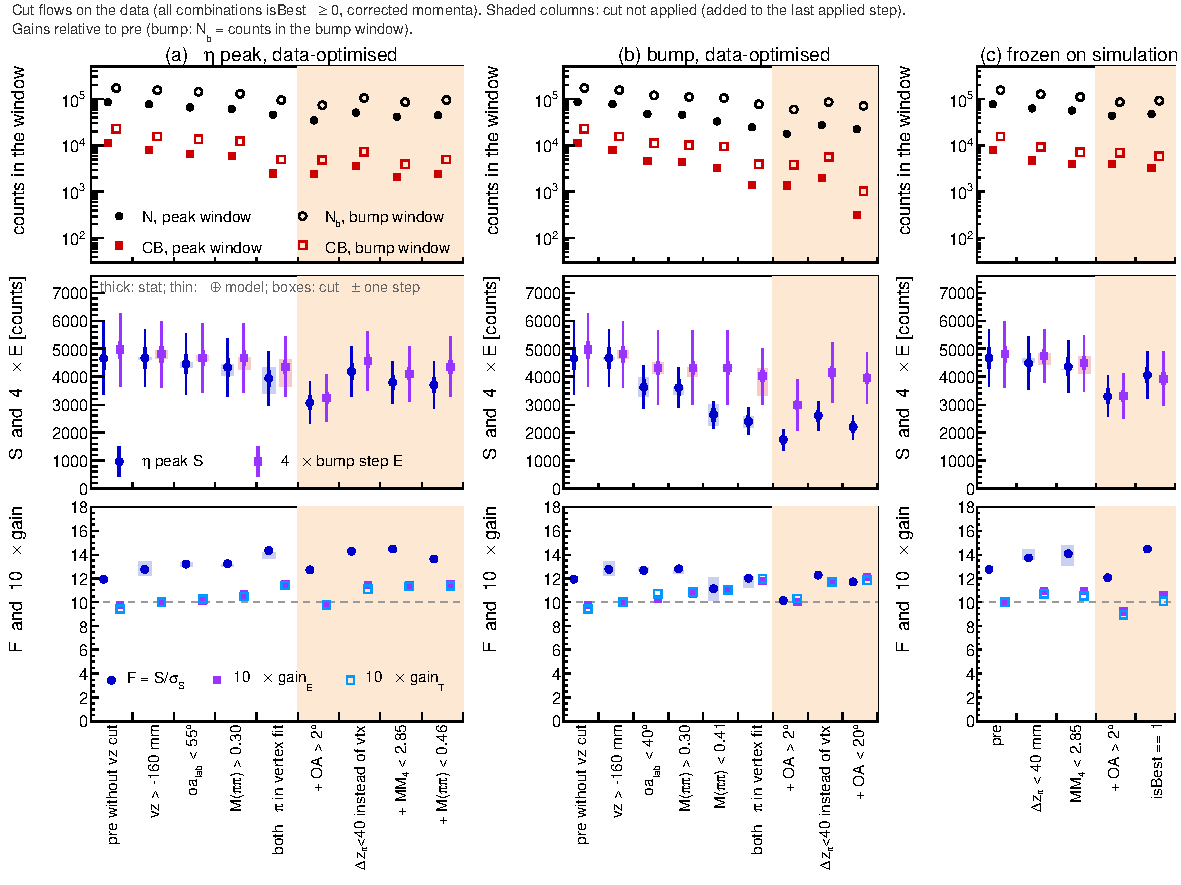
\includegraphics[width=\textwidth]{figs_exp/opt_cutflow_cnt.pdf}
\caption{Cut flows on the data (isBest $\ge0$): (a) $\eta$-peak selection, (b) bump selection, (c) frozen simulation
selections. Selection: data; start point \ptthreecap{}, a reconstructed event vertex ($\vz>-500$\,mm), particles identified by the START-free velocity \betanew (pions within $3\sigma$, leptons within $5\sigma$ of the expected band; leptons with a RICH ring), energy-loss-corrected momenta for all four tracks, all stored combinations of each event (isBest $\ge0$), no target-region cut; cuts added step by step: (a) $\vz>-160$\,mm (giving ``pre''), angle between the \pipi and the \ee momenta in the laboratory $\alab<55^\circ$, $\Mpipi>0.30$\,\GeVcc, both pion tracks used in the fit of the event vertex; (b) $\vz>-160$\,mm, $\alab<40^\circ$, $\Mpipi>0.30$\,\GeVcc, $\Mpipi<0.41$\,\GeVcc, both pions in the vertex fit; (c) from ``pre'': both pion tracks within 40\,mm of the event vertex along the beam ($\dzpi<40$\,mm), then $\MMfour<2.85$\,\GeVcc; shaded, not applied: (a) OA$>2^\circ$, $\dzpi<40$\,mm instead of the vertex flag, $\MMfour<2.85$\,\GeVcc, $\Mpipi<0.46$\,\GeVcc; (b) OA$>2^\circ$, $\dzpi<40$\,mm instead of the vertex flag, OA$<20^\circ$; (c) OA$>2^\circ$, isBest $=1$; boxes, the cut of the step moved to (a) $-170$/$-150$\,mm, $50^\circ$/$60^\circ$, 0.28/0.32\,\GeVcc, at least one pion/all four tracks in the vertex fit; (b) $-170$/$-150$\,mm, $35^\circ$/$45^\circ$, 0.28/0.32\,\GeVcc, 0.40/0.42\,\GeVcc, at least one pion/all four tracks; (c) 30/60\,mm, 2.80/2.90\,\GeVcc; data peak window $0.53364\le\Mfour<0.55416$\,\GeVcc, data bump window $0.4550\le\Mfour<0.5225$\,\GeVcc. Top: counts $N$ and CB in the peak window (full) and in the bump window (open). Middle: $S\pm$stat (thin: $\oplus$
model spread) and $4\times E$; boxes: the cut of this step moved one step down / up. Bottom: $F$ and $10\times$gain$_E$,
$10\times$gain$_T$ relative to ``pre''. Shaded columns: cuts not applied, each added to the last applied step. CB with
$k=1$; counts, not normalised to luminosity.}
\label{fig:opt_cutflow}
\end{figure}

\subsection{Vertex cuts}
\label{sec:vertex}
\textbf{Event vertex.} The $\eta$ signal per $\vz$ slice (base ``pre'' without the $\vz$ cut) is given in
Table~\ref{tab:vzslices}: below $-160$\,mm there is no $\eta$, neither in the peak nor in the tagged sample, while the CB
share there is 0.39--0.46. All counts with $\vz\le-160$\,mm together give $S=-19\pm133$. The adopted cut keeps all of the
signal ($\varepsilon_S=1.004\pm0.029$, $\varepsilon_B=0.896$) and raises $F$ from 11.93 to 12.74. A tighter cut,
$\vz>-150$\,mm, gives $F=13.43$ ($\varepsilon_S=0.991\pm0.039$, $\varepsilon_B=0.794$), but the difference lies inside the
bias range of a data choice (\S\ref{sec:bias}); $-160$\,mm is kept ($-140$: 13.24, $\varepsilon_S=0.884\pm0.045$;
$-130$: 11.53). The CB-rich counts below $-160$\,mm are target material: in the empty-target runs measured after the first draft the walls
give 0.76--0.87 of the unlike-sign counts there (last column of Table~\ref{tab:vzslices}; \S\ref{sec:walls}). In $-160$\dots$-150$\,mm,
where 0.76 of the counts are wall counts, the $\eta$ per count is $0.12\pm0.28$ ($S$) and $0.25\pm0.08$ ($T$) of the average, about the
$1-0.76=0.24$ that the hydrogen counts alone would give if the walls made no $\eta$. The
mandatory cut $\vz>-500$\,mm itself is measured in \S\ref{sec:vtxeff}: it keeps $0.994\pm0.021$ of the $\eta$.

\begin{table}[H]
\centering
\caption{$\eta$ signal per event-vertex slice, data, base ``pre'' without the $\vz$ cut, all combinations
(isBest $\ge0$). $S$: \Pmain content of the peak; ``rel.'': signal per peak-window count relative to all $z$; $T$:
ECAL-tagged $\eta$; CB$/N$ in the peak window ($k=1$); wall share: share of the target walls in the unlike-sign counts of ``pre''
(all \Mfour), from the empty-target runs of days 034, 047, 065 (raw, luminosity-weighted; Part~III, verifier vw2b; data only; added after
the first draft, \S\ref{sec:walls}). Counts, not normalised to luminosity (notation: Table~\ref{tab:notation}).}
\label{tab:vzslices}
\small
\begin{tabular}{@{}l r r r r r@{}}
\toprule
$\vz$ slice [mm] & $S$ & $S$ rel. & $T$ & CB$/N$ & wall share \\
\midrule
$-500$\dots$-200$ & $-12\pm36$ & $\approx0$ & $7\pm7$ & 0.46 & -- \\
$-200$\dots$-170$ & $-19\pm76$ & $\approx0$ & $3\pm14$ & 0.45 & 1.01 (normaliser) \\
$-170$\dots$-160$ & $9\pm104$ & $\approx0$ & $-14\pm19$ & 0.39 & 0.87 \\
$-160$\dots$-150$ & $54\pm127$ & $0.12\pm0.28$ & $84\pm28$ (rel.\ $0.25\pm0.08$) & 0.28 & 0.76 \\
$-150$\dots$-90$ & -- & 0.8--1.6 & rel.\ 1.0--1.5 & 0.04--0.15 & 0.05--0.30 \\
\bottomrule
\end{tabular}
\end{table}

\textbf{Pions in the vertex fit} (a reconstruction flag): $\ge1$ pion $F=13.20$ ($\varepsilon_S=1.002\pm0.021$,
$\varepsilon_B=0.940$), both pions $F=14.31$ ($\varepsilon_S=0.940\pm0.041$, $\varepsilon_B=0.708$), all four tracks 13.93
($\varepsilon_S=0.783\pm0.045$). The flag removes 59\,\% of the CB but only 28\,\% of the unlike-sign counts (\S\ref{sec:cbshare}).
Its efficiency comes from the simulation (Part~III compares it on its base S0/``pre'': data $0.941\pm0.052$ against simulation 0.940 for the
$\eta$ peak; this report gives $0.940\pm0.041$ in the data on the base ``peak nominal'').

\textbf{The geometric alternative $\dzpi$} (Fig.~\ref{fig:prep_dzpi}, Table~\ref{tab:prep_dzpi}, Table~\ref{tab:dzthr}).
Measured on the data peak, $\varepsilon_S(\dzpi<40\,\mathrm{mm})=0.961\pm0.034\pm0.019$
(pass/fail fits, base ``pre''), $0.952\pm0.040\pm0.014$ with OA$>2^\circ$ and $0.978\pm0.034\pm0.011$ with isBest $=1$ (the
binned \dzpi shape of the signal in Fig.~\ref{fig:prep_dzpi} puts about 98\,\% below 40\,mm, a less direct estimate); the cut
keeps 0.81 of the unlike-sign counts in the windows but 0.58 of the like-sign counts (CB kept 0.60). The simulation gives 0.9625
for $\eta\to\ppee$ alone (class 5) and 0.963 for direct decay plus conversion (classes 4+5), both in the simulation peak
window, and 0.955 for classes 4+5 over all \Mfour (Table~\ref{tab:dzthr}); data and simulation agree, but only to the 4\,\%
precision of the data. The best data threshold is 30\,mm ($F=14.48$,
$\varepsilon_S=0.967\pm0.040$, $\sqrt{\varepsilon_B}=0.854$); 20\,mm gives 13.67, 40\,mm 13.74, 60\,mm 13.59; 10 and 15\,mm lose.

\begin{table}[H]
\centering
\caption{Signal efficiency of $\dzpi<X$ on the data $\eta$ peak (\Pmain pass/fail fits, stat $\pm$ model), base ``pre'',
all combinations (isBest $\ge0$), and the share of the unlike-sign counts in the data peak window that pass; last row:
simulated efficiency (all \Mfour, direct + conversion, quoted from Part~I; no CB there). Not normalised to luminosity.}
\label{tab:dzthr}
\small
\setlength{\tabcolsep}{3pt}
\begin{tabular}{@{}l c c c c c c c c@{}}
\toprule
$X$ [mm] & 10 & 15 & 20 & 30 & 40 & 60 & 100 & 150 \\
\midrule
$\varepsilon_S$ data & $0.438$ & $0.684$ & $0.819$ & $0.967$ & $0.961$ & $0.995$ & $0.990$ & $0.989$ \\
\quad stat & $\pm0.037$ & $\pm0.043$ & $\pm0.043$ & $\pm0.040$ & $\pm0.034$ & $\pm0.028$ & $\pm0.020$ & $\pm0.016$ \\
\quad model & $\pm0.026$ & $\pm0.023$ & $\pm0.012$ & $\pm0.018$ & $\pm0.019$ & $\pm0.009$ & $\pm0.009$ & $\pm0.009$ \\
counts kept (peak window) & 0.294 & 0.473 & 0.597 & 0.742 & 0.812 & 0.883 & 0.937 & 0.962 \\
$\varepsilon$ simulation & -- & -- & 0.827 & 0.924 & 0.955 & 0.980 & 0.991 & 0.996 \\
\bottomrule
\end{tabular}
\end{table}

% wr_prep_dzpi_cnt.tex: copy of wr_prep_dzpi.tex with "rows" -> "counts" (analyst, 15 Nov 2026; Part II writer, integ4)
% wr_prep_dzpi.tex -- copy of prep_dzpi.tex, tabular scaled to the text width by the report writer; original written by plots/exp_report/prep_dzpi.C (numbers: tables_exp/prep_dzpi.txt)
\begin{table}[H]
\centering\small
\setlength{\tabcolsep}{4pt}
\caption{Pion-vertex distance $\Delta z_\pi=\max(|z_{\pi^+}-v_z|,|z_{\pi^-}-v_z|)$ in the data: pass fraction of $\Delta z_\pi<40$~mm. Counts: all stored combinations (isBest $\geq 0$) unless stated, corrected momenta, PT3, $v_z>-160$~mm. Fractions of the counts: data peak window 0.53364--0.55416, side bands 0.5225--0.53364 and 0.55416--0.56530~GeV/$c^2$, errors with the event-group correlation. Signal: $\varepsilon_S=S_\mathrm{pass}/(S_\mathrm{pass}+S_\mathrm{fail})$ from $P_\mathrm{main}$ fits (stat $\pm$ model). Not normalised to luminosity. Simulation: values copied from the simulation study (no combinatorial background there).}
\label{tab:prep_dzpi}
\resizebox{\textwidth}{!}{%
\begin{tabular}{llc}
\toprule
Sample & Selection & pass fraction $\Delta z_\pi<40$~mm \\
\midrule
$e^+e^-$ counts, all $M_4$ & pre & $0.860\pm0.000$ \\
$e^+e^-$ counts, peak window & pre & $0.812\pm0.001$ \\
$e^+e^-$ counts, lower side band & pre & $0.798\pm0.002$ \\
$e^+e^-$ counts, upper side band & pre & $0.811\pm0.002$ \\
$e^\pm e^\pm$ counts, 0.5225--0.5653 & pre & $0.580\pm0.003$ \\
$e^+e^-$ counts, bump window & pre & $0.812\pm0.001$ \\
\midrule
$\eta$ peak signal $\varepsilon_S$ & pre & $0.961\pm0.034\pm0.019$ \\
$\eta$ peak signal $\varepsilon_S$ & pre + OA$>2^\circ$ & $0.952\pm0.040\pm0.014$ \\
$\eta$ peak signal $\varepsilon_S$ & pre, isBest $=1$ & $0.978\pm0.034\pm0.011$ \\
$\eta$ peak signal $\varepsilon_S$ & peak nominal & $0.965\pm0.033\pm0.021$ \\
$\eta$ peak signal $\varepsilon_S$ & bump nominal & $0.984\pm0.039\pm0.051$ \\
$\eta$ peak signal $\varepsilon_S$ & no $v_z$ cut + $\alpha_\mathrm{lab}<55^\circ$, $M_{\pi\pi}>0.30$ & $0.968\pm0.036\pm0.025$ \\
\midrule
Simulation, $\eta\to\pi^+\pi^-e^+e^-$ (sim window) & pre (DIRECT) & $0.9625\pm0.0005$ \\
Simulation, direct / conversion / total (all $M_4$) & pre & $0.955$ / $0.954$ / $0.955\pm0.006$ \\
Simulation, physical background in the peak window & pre & $0.827\pm0.007$ \\
\bottomrule
\end{tabular}}
\end{table}


\begin{figure}[H]
\centering
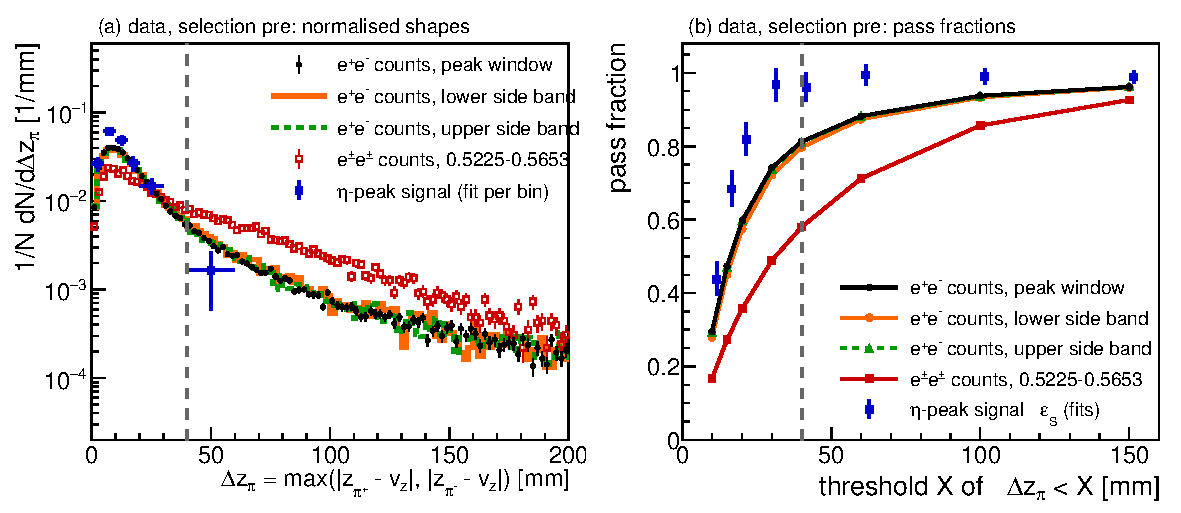
\includegraphics[width=\textwidth]{figs_exp/prep_dzpi_cnt.pdf}
\caption{Distance of the pion tracks from the event vertex, $\dzpi=\max(|z_{\pi^+}-\vz|,|z_{\pi^-}-\vz|)$, data, selection
``pre'' (all combinations isBest $\ge0$, \code{cor_ok} $=1$, PT3, $\vz>-500$\,mm and $\vz>-160$\,mm). Selection: data with the base cuts \ptthreecap{}, an event vertex reconstructed ($\vz>-500$\,mm) and inside the target region ($\vz>-160$\,mm), particles identified by the START-free velocity \betanew (pions within $3\sigma$, leptons within $5\sigma$ of the expected band; leptons with a RICH ring), energy-loss-corrected momenta for all four tracks, all stored \ppee combinations of each event (isBest $\ge0$), no further cut (together ``pre''); unlike-sign counts in the data peak window $0.53364\le\Mfour<0.55416$\,\GeVcc, in the lower side band 0.5225--0.53364 and in the upper side band 0.55416--0.56530\,\GeVcc; like-sign counts in 0.5225--0.5653\,\GeVcc; the $\eta$-peak signal from fits in 0.5225--0.6100\,\GeVcc per \dzpi bin. (a) Shapes, unit area
(including $\dzpi>200$\,mm), 2\,mm bins: unlike-sign counts in the data peak window (black), lower side band (orange), upper
side band (green dashed), like-sign counts in 0.5225--0.5653\,\GeVcc (red), and the $\eta$-peak signal from \Pmain fits in
\dzpi bins (blue; bins with $S\le0$ not drawn on the log scale). (b) Fraction of counts with $\dzpi<X$ for the same samples;
blue: $\varepsilon_S$ from pass/fail fits, stat $\oplus$ model. Dashed: the frozen cut 40\,mm. CB $=2\sqrt{N_{++}N_{--}}$, $k=1$;
counts, not normalised to luminosity.}
\label{fig:prep_dzpi}
\end{figure}

\begin{figure}[H]
\centering
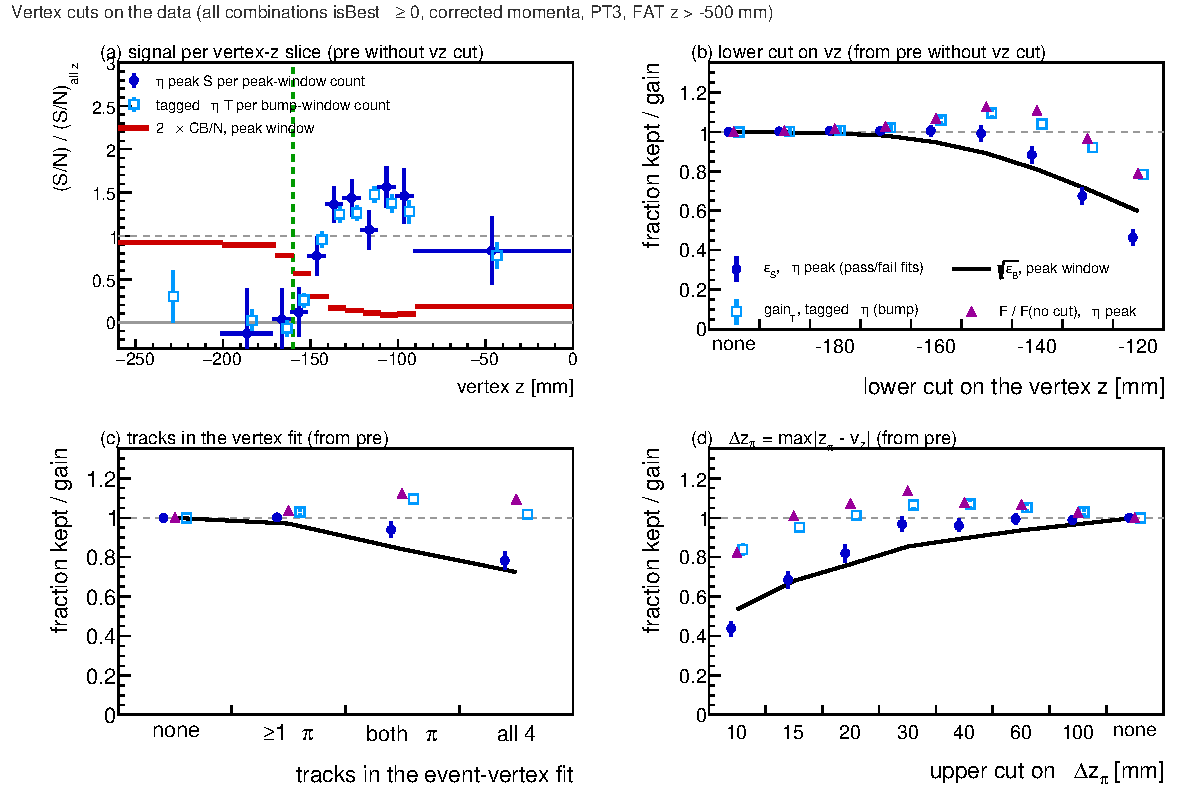
\includegraphics[width=\textwidth]{figs_exp/opt_vertex_cnt.pdf}
\caption{Vertex cuts on the data (isBest $\ge0$). Selection: data, \ptthreecap{}, a reconstructed event vertex ($\vz>-500$\,mm), particles identified by the START-free velocity \betanew (pions within $3\sigma$, leptons within $5\sigma$ of the expected band; leptons with a RICH ring), energy-loss-corrected momenta for all four tracks, all stored combinations of each event (isBest $\ge0$); (a), (b): nothing more (``pre'' without its cut $\vz>-160$\,mm), (a) in slices of \vz, (b) with a lower cut on \vz at the values on the axis; (c), (d): in addition $\vz>-160$\,mm (``pre''), (c) no, at least one pion, both pions or all four tracks in the event-vertex fit, (d) \dzpi below the values on the axis; $S$ per count in the data peak window $0.53364\le\Mfour<0.55416$\,\GeVcc, $T$ (an ECAL photon identified as a photon with $0.8<\beta<1.2$ and energy above 100\,MeV (of up to three such photons the one with $M(\ee\gamma)$ closest to 0.140\,\GeVcc), $0.119\le M(\ee\gamma)<0.173$\,\GeVcc and $\Mee<0.10$\,\GeVcc) per count in the data bump window $0.4550\le\Mfour<0.5225$\,\GeVcc. (a) Signal per $\vz$ slice relative to all $z$: $\eta$-peak $S$ per
peak-window count (blue), tagged $T$ per bump-window count (light blue), $2\times$CB$/N$ in the peak window (red); green: the
adopted cut $\vz>-160$\,mm (base ``pre'' without $\vz$ cut; the $-500$\dots$-200$\,mm point is off scale, $-0.4\pm1.2$).
(b) lower cut on $\vz$, (c) tracks in the event-vertex fit, (d) \dzpi: $\varepsilon_S$ of the peak, $\sqrt{\varepsilon_B}$,
gain$_T$ of the tagged $\eta$ and $F/F(\text{no cut})$. Counts, not normalised to luminosity.}
\label{fig:opt_vertex}
\end{figure}

\subsection{Sculpting}
\label{sec:sculpt}
\textbf{Procedure} (as in the first study). Three sets of counts are used: unlike-sign counts, like-sign counts, and mixed counts
made of the pion pair of one combination and the lepton pair of another event group (20 offsets, pool of the 3\,344\,847 ``pre''
counts with $0.35\le\Mfour<0.95$\,\GeVcc; \Mfour, \alab, \MMfour and \aeta recomputed, closure on unmixed combinations $2\times10^{-6}$\,GeV). For each cut value the
pass fraction against \Mfour is measured. Flag \textbf{G}: the like-sign pass fraction turns on inside the fit range.
Flag \textbf{M}: the smooth background of ``pre'' multiplied by the mixed pass fraction and fitted with Gaussian + pol2
gives a fake content $|S_{\mathrm{fake}}|>92$ counts ($0.25\,\sigma_S$ of ``pre''). Like-sign null fits are done in addition.

\textbf{Result} (Table~\ref{tab:sculpt}, Figs.~\ref{fig:sculpt_pass}, \ref{fig:sculpt_fake}). Upper \Mpipi cuts, upper
\MMfour cuts other than 2.85, and $\aeta>150^\circ$ sculpt. The $\aeta$ cut is a mass band-pass: its pass fraction rises from
0 at 0.40 to 1 at 0.50\,\GeVcc and falls above 0.62\,\GeVcc. $\MMfour<2.85$ carries flag G only (like-sign turn-on at
0.476--0.598); inside PEAK the fake content is $+48\pm27$ counts (1.1\,\% of $S$). \alab, lower \Mpipi, \dzpi, the vertex flags and
OA do not sculpt. All like-sign null fits of the named selections are consistent with zero (e.g.\ PEAK $++$ $20\pm40$,
$--$ $28\pm81$).

\tipbox{\textbf{Two implementations of $S_{\mathrm{fake}}$ disagree by up to 70 counts} (35, 25, 70, 60 counts for PEAK, DIRECT,
pre + vertex, peak nominal + vertex; 16 and $-2$ for peak nominal and the X17 band). The results chapter repeated the test
(pass fraction relative to ``pre'' times the pol2 of the Poisson fit of ``pre'') and finds $S_{\mathrm{fake}}=+83\pm26$
(PEAK), $+40\pm23$ (DIRECT), $+83\pm27$ (pre + vertex), $+73\pm30$ (peak nominal + vertex), $+18\pm35$ (peak nominal),
$+15\pm22$ (X17 band), against $+48\pm27$, $15\pm23$, $13\pm27$, $13\pm79$, $2\pm72$, $17\pm16$ here. Neither
implementation was re-derived by the verifiers. The mixed spectrum itself is not exactly pol2 in the fit range
(self-fit $-270\pm67$ counts), so $S_{\mathrm{fake}}$ has a method uncertainty of tens of counts. Both versions agree that
the pion-vertex cuts and $\MMfour<2.85$ create at most $+40$ to $+83$ counts ($\le1.9$\,\% of $S$, $\le0.27$ stat), far below
the model spread; three selections lie just above the 0.25-stat flag threshold in the second version. Quote it as a
small one-sided systematic of PEAK, DIRECT and the ``+ vertex'' selections.}

\begin{table}[H]
\centering
\caption{Fake $\eta$-peak content $S_{\mathrm{fake}}$ (counts) made by a cut from a smooth background (pass fraction of the mixed counts
times the background of ``pre'', fitted with Gaussian + pol2), base ``pre'', data, isBest $\ge0$. Flags: G, like-sign
turn-on in the fit range; M, $|S_{\mathrm{fake}}|>92$ counts. Not normalised to luminosity.}
\label{tab:sculpt}
\small
\begin{tabular}{@{}l l l l@{}}
\toprule
Single cut & $S_{\mathrm{fake}}$ & Named selection & $S_{\mathrm{fake}}$ \\
\midrule
$\alab<25$--$70^\circ$ & $-5$\dots$63$ & peak nominal & $2\pm72$ \\
$\Mpipi>0.28$--0.38 & $-71$\dots$-1$ & peak nominal + vertex & $13\pm79$ \\
$\Mpipi<0.39$--0.42 & 92--116 (M) & DIRECT & $15\pm23$ \\
$\Mpipi<0.43$--0.44 & 39 / $-42$ (G) & PEAK & $48\pm27$ \\
$\Mpipi<0.45$--0.50 & $-140$\dots$-397$ (G, M) & pre + vertex & $13\pm27$ \\
$\MMfour<2.60$--2.80 & 120--246 (M; G at 2.60--2.70) & X17 band & $17\pm16$ \\
$\MMfour<2.85$ & $29\pm21$ (G) & bump nominal & $307\pm31$ (M) \\
$\MMfour<2.90$ & $-220$ (G, M) & bump nominal + vertex & $224\pm29$ (M) \\
$\aeta>100/120/140^\circ$ & $-3/-10/-48$ & slides & $-120\pm39$ (M) \\
$\aeta>150^\circ$ / $>160^\circ$ & $-232$ / $-2181$ (M) & old code & $269\pm30$ (M) \\
$\dzpi<10$--100\,mm & $-20$\dots$66$ & & \\
vertex-fit categories; OA cuts & 13\dots41; below 41 & & \\
\bottomrule
\end{tabular}
\end{table}
The large fakes of bump nominal (+307) come from its cut $\Mpipi<0.41$; they matter for a peak fit but not for the
bump edge fits, which work in \Mpipi slices.

\begin{figure}[H]
\centering
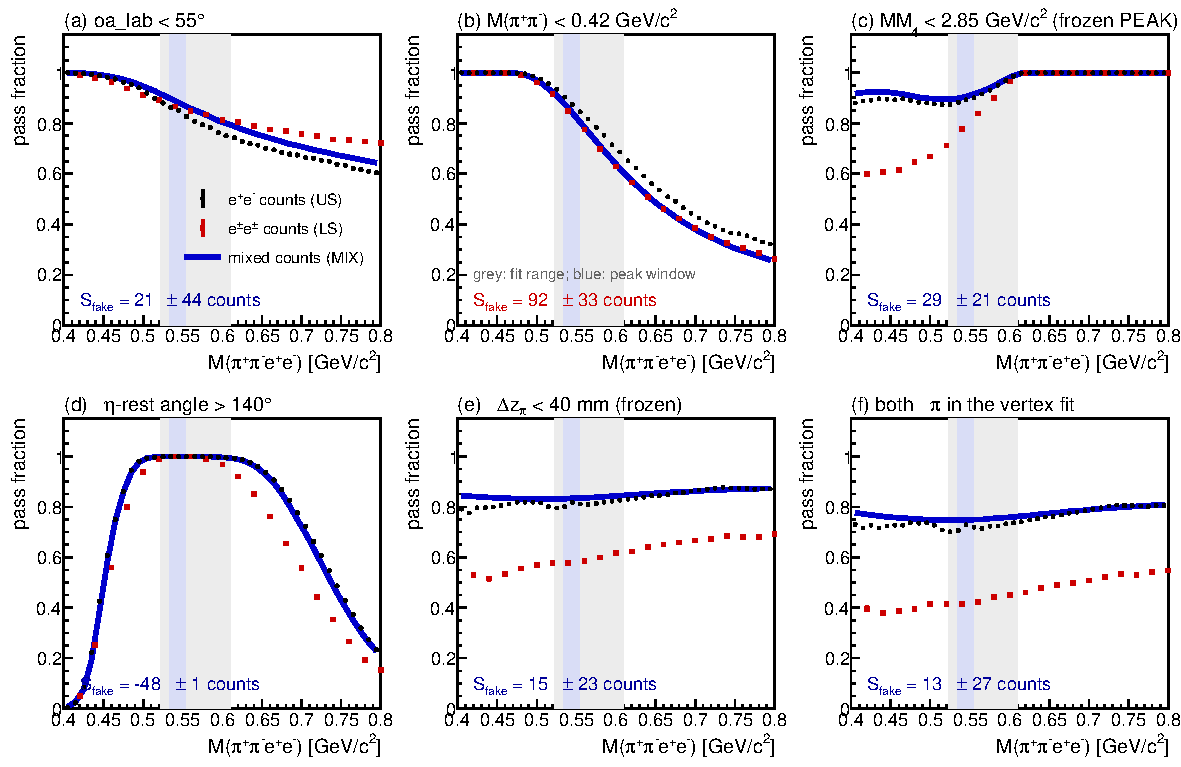
\includegraphics[width=\textwidth]{figs_exp/opt_sculpt_passfrac_cnt.pdf}
\caption{Pass fraction against \Mfour of six cuts for unlike-sign counts (black), like-sign counts (red) and mixed counts (pion
pair and lepton pair from different events; blue line); base ``pre'', data, isBest $\ge0$. Selection: data with the base cuts \ptthreecap{}, an event vertex reconstructed ($\vz>-500$\,mm) and inside the target region ($\vz>-160$\,mm), particles identified by the START-free velocity \betanew (pions within $3\sigma$, leptons within $5\sigma$ of the expected band; leptons with a RICH ring), energy-loss-corrected momenta for all four tracks, all stored \ppee combinations of each event (isBest $\ge0$) (together ``pre''); the six cuts: (a) $\alab<55^\circ$ (angle between the \pipi and the \ee momenta in the laboratory), (b) $\Mpipi<0.42$\,\GeVcc, (c) $\MMfour<2.85$\,\GeVcc, (d) $\eta$-rest angle $\aeta>140^\circ$, (e) $\dzpi<40$\,mm, (f) both pion tracks used in the fit of the event vertex; mixed counts: the pion pair of an unlike-sign ``pre'' count with the lepton pair of a count of another event, both from the ``pre'' counts with $0.35\le\Mfour<0.95$\,\GeVcc. Grey: \Pmain fit range; blue
band: data peak window. $S_{\mathrm{fake}}$ = Gaussian content that the mixed pass fraction makes from the smooth
background of ``pre'' (red: flagged). (d) The $\aeta$ cut is a band-pass in \Mfour. Counts, not normalised to luminosity.}
\label{fig:sculpt_pass}
\end{figure}

\begin{figure}[H]
\centering
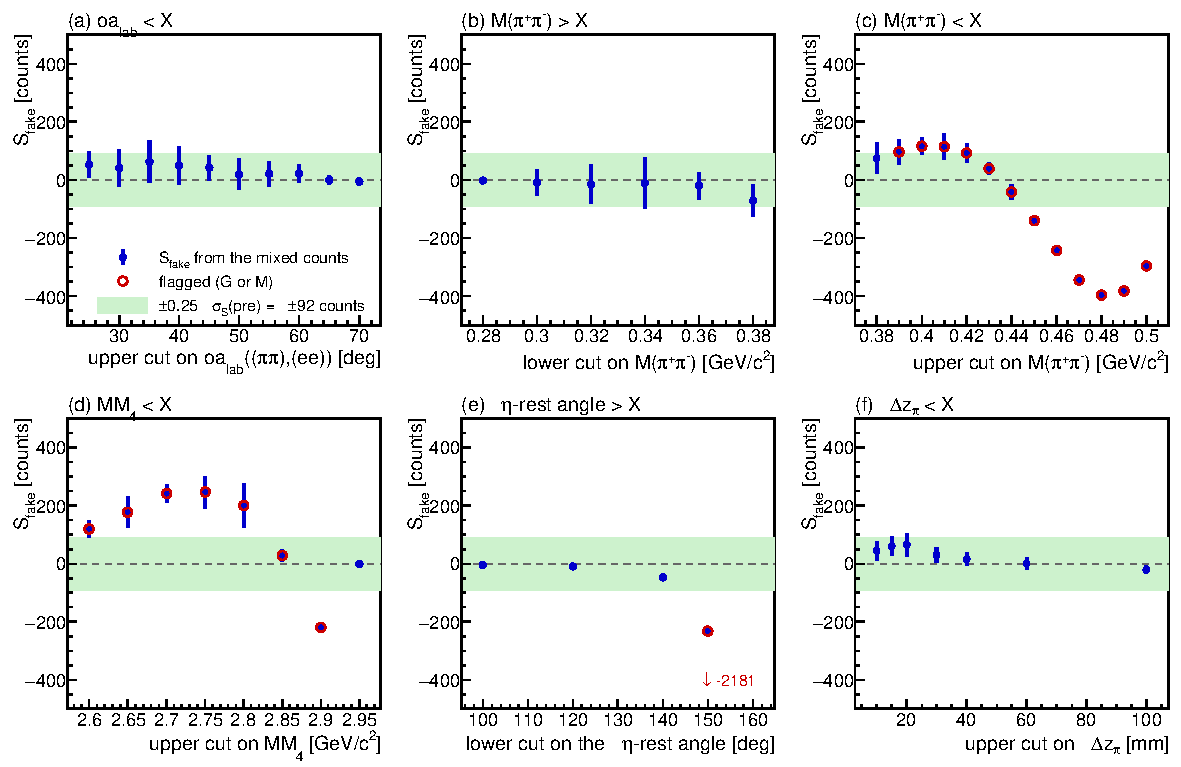
\includegraphics[width=\textwidth]{figs_exp/opt_sculpt_fake_cnt.pdf}
\caption{Fake $\eta$-peak content $S_{\mathrm{fake}}$ made by a cut on a smooth background against the cut value (data,
base ``pre'', isBest $\ge0$). Selection: data with the base cuts \ptthreecap{}, an event vertex reconstructed ($\vz>-500$\,mm) and inside the target region ($\vz>-160$\,mm), particles identified by the START-free velocity \betanew (pions within $3\sigma$, leptons within $5\sigma$ of the expected band; leptons with a RICH ring), energy-loss-corrected momenta for all four tracks, all stored \ppee combinations of each event (isBest $\ge0$) (together ``pre''); one cut per panel at the values on the horizontal axis: (a) upper cut on the angle \alab between the \pipi and the \ee momenta in the laboratory, (b) lower and (c) upper cut on \Mpipi, (d) upper cut on \MMfour, (e) lower cut on the $\eta$-rest angle \aeta, (f) upper cut on \dzpi; mixed counts from the unlike-sign ``pre'' counts with $0.35\le\Mfour<0.95$\,\GeVcc; fake content fitted with the frozen Gaussian (0.5439\,\GeVcc, 5.4\,\MeVcc) and a second-order polynomial in 0.5225--0.6100\,\GeVcc. Green: $\pm0.25\,\sigma_S(\mathrm{pre})=\pm92$ counts. Red circles: flagged (like-sign turn-on in
the fit range or $|S_{\mathrm{fake}}|>92$). Arrows: values outside the frame. Counts.}
\label{fig:sculpt_fake}
\end{figure}

\subsection{Optimisation bias}
\label{sec:bias}
\textbf{Procedure.} A grid of 840 working points on top of ``pre'' (\alab, lower \Mpipi cut, pions in the vertex fit, \dzpi,
$\MMfour<2.85$ or none) is evaluated on halves of the data: the fold split and 40 random halvings of the event groups. On
half A a point $c_A$ is chosen by one of four fixed rules and measured on half B, and vice versa. The rules
(\code{opt_bias.C}): \emph{best-$F$}, the point with the largest $F_A$; \emph{loose}, the point with the most counts in the
peak window among the points with $F_A\ge F_{A,\mathrm{best}}-1$; \emph{pure}, the point with the largest $S/B$ among the same
points; \emph{nominal}, the self-consistent plateau centre of the first study (starting from $\alab<50^\circ$, each variable
is moved to the centre of its values with $F\ge F_{\mathrm{best}}-1$ in an N$-$1 scan around the current point, or left open;
repeated until stable, at most 8 times). The bias is
\begin{equation}
b(F)=\tfrac12\left[\left(F_A(c_A)-F_B(c_A)\right)+\left(F_B(c_B)-F_A(c_B)\right)\right],
\label{eq:bias}
\end{equation}
and the \emph{independent gain} of a rule is $F$ on the half not used for the choice minus $F(\mathrm{pre})$ there (for a
fixed point simply $F(\text{point})-F(\mathrm{pre})$), scaled by $\sqrt2$ to the full sample. $\MMfour<2.85$ is never chosen
by the rules (flag G).

\textbf{Result} (Table~\ref{tab:opt_bias}, Fig.~\ref{fig:opt_bias}). On the full-sample scale the bias is 0.42 (nominal), 0.81
(loose), 1.15 (pure) and 1.58 (best-$F$) units of $F$ (40 random halvings; the fold halving gives 0.61/1.03/1.17/1.85 on the
full-sample scale, 0.43/0.73/0.83/1.31 per half; first study, kinematic grid without $\vz$ cut, per half: 0.47/0.16/0.96/1.13). The nominal rule applied blind gains $+1.36$ over ``pre'' and lands by itself on
$\dzpi<40$\,mm (``$\alab<55^\circ$, $\Mpipi>0.30$, $\ge1$ pion in the vertex fit, $\dzpi<40$'' in 40 of 80 halves). The frozen PEAK
gains $+1.35$, DIRECT $+1.00$. The fixed point peak nominal + vertex gains $+1.57$, but it was chosen with all data:
minus the bias of the nominal rule it is about $+1.15$. The best-$F$ point of the full sample ($\alab<50^\circ$, $\Mpipi>0.30$,
$\dzpi<30$\,mm) has $F=14.98$, 0.9 above PEAK and less than the expected best-$F$ bias: no evidence for a better selection. The
errors of $b$ are too small (the halvings share events).

% opt_bias.tex -- written by plots/exp_report/opt_bias.C (numbers: tables_exp/opt_bias.txt)
\begin{table}[H]
\centering\small
\setlength{\tabcolsep}{4pt}
\caption{Optimisation bias of data-driven choices of the $\eta$-peak selection and the gain over pre on independent events. 40 random halvings of the event groups; the working point is chosen on one half by a fixed rule (grid of 840 points on top of pre: $\alpha_\mathrm{lab}$, $M_{\pi\pi}$ lower cut, pions in the vertex fit, $\Delta z_\pi$, MM$_4<2.85$ or none; MM$_4<2.85$ is never chosen by the rules because of its sculpting flag) and evaluated on the other. $b$ = mean of $\frac12[(F_A(c_A)-F_B(c_A))+(F_B(c_B)-F_A(c_B))]$; gain = $F$ on the other half minus $F$(pre) there; per half and scaled by $\sqrt2$ to the full sample. Errors: rms$/\sqrt{n}$ (too small, the halvings share events). $^*$For a fixed point the halving test gives $b=0$ by construction: it cannot see a choice made on all data, so the points chosen on these data (peak nominal, + vertex, pre + vertex, + $\Delta z_\pi<40$) still carry the bias of the rule that found them (nominal rule: 0.42 on the full-sample scale); only the frozen DIRECT and PEAK are free of it. Data, isBest $\geq0$, $P_\mathrm{main}$.}
\label{tab:opt_bias}
\begin{tabular}{lcccc}
\toprule
Rule or point & $b(F)$ per half & $b(F)\times\sqrt2$ & gain per half & gain $\times\sqrt2$ \\
\midrule
nominal (data-driven) & $0.29\pm0.05$ & 0.42 & $0.96\pm0.03$ & 1.36 \\
loose (data-driven) & $0.57\pm0.05$ & 0.81 & $0.49\pm0.04$ & 0.70 \\
pure (data-driven) & $0.81\pm0.06$ & 1.15 & $0.36\pm0.04$ & 0.51 \\
best-F (data-driven) & $1.12\pm0.07$ & 1.58 & $0.83\pm0.06$ & 1.17 \\
\midrule
peak nominal (chosen on data) & 0$^*$ & -- & $0.35$ & 0.50 \\
peak nominal + vertex (chosen on data) & 0$^*$ & -- & $1.11$ & 1.57 \\
pre + vertex (chosen on data) & 0$^*$ & -- & $1.11$ & 1.58 \\
peak nominal + $\Delta z_\pi<40$ (chosen on data) & 0$^*$ & -- & $1.10$ & 1.55 \\
DIRECT (frozen on simulation) & 0$^*$ & -- & $0.71$ & 1.00 \\
PEAK (frozen on simulation) & 0$^*$ & -- & $0.96$ & 1.35 \\
\bottomrule
\end{tabular}
\end{table}


\begin{figure}[H]
\centering
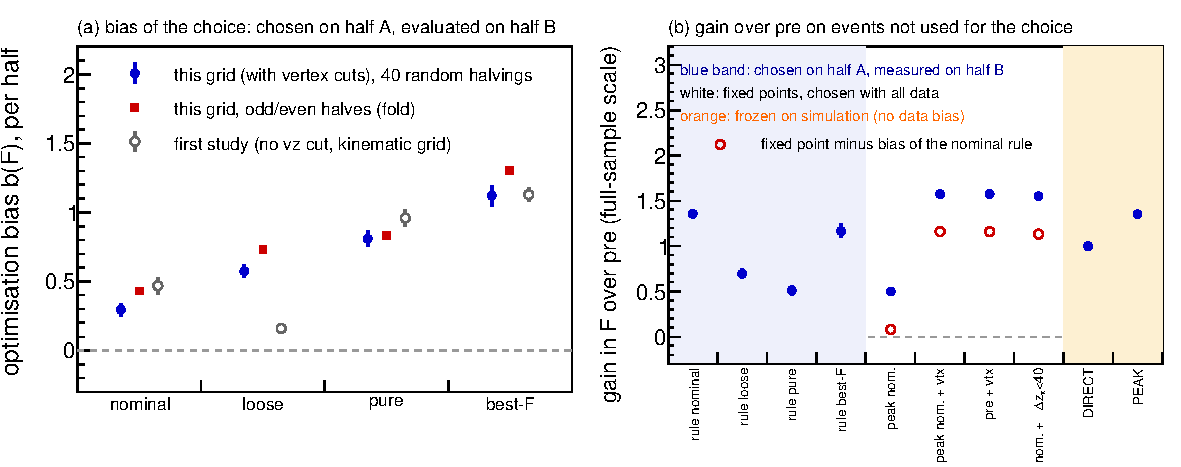
\includegraphics[width=\textwidth]{figs_exp/opt_bias.pdf}
\caption{Optimisation bias of data-driven peak selections (data, isBest $\ge0$, \Pmain). Selection: data; 840 working points on top of the base cuts \ptthreecap{}, an event vertex reconstructed ($\vz>-500$\,mm) and inside the target region ($\vz>-160$\,mm), particles identified by the START-free velocity \betanew (pions within $3\sigma$, leptons within $5\sigma$ of the expected band; leptons with a RICH ring), energy-loss-corrected momenta for all four tracks, all stored \ppee combinations of each event (isBest $\ge0$) (together ``pre''): the angle \alab between the \pipi and the \ee momenta in the laboratory below 40, 45, 50, 55, 60 or $65^\circ$ or no cut, $\times$ \Mpipi above 0.30, 0.32 or 0.34\,\GeVcc or no cut, $\times$ both pions, at least one pion or no requirement in the event-vertex fit, $\times$ \dzpi below 20, 30, 40 or 60\,mm or no cut, $\times$ $\MMfour<2.85$\,\GeVcc or no cut; halves: odd/even event groups and 40 random halvings of the event groups; (b) fixed points: peak nominal ($\alab<55^\circ$, $\Mpipi>0.30$\,\GeVcc), peak nominal + vertex, pre + vertex, peak nominal and $\dzpi<40$\,mm; frozen: DIRECT ($\dzpi<40$\,mm), PEAK ($\dzpi<40$\,mm, $\MMfour<2.85$\,\GeVcc); grey: the first data study, its kinematic grid without vertex cuts and without the cut $\vz>-160$\,mm; fits in 0.5225--0.6100\,\GeVcc. (a) Bias $b(F)$ per half for
four fixed rules choosing a working point on one half (grid of 840 points on top of ``pre'', including vertex cuts and
$\MMfour<2.85$/none; \MMfour never chosen): 40 random halvings (blue), odd/even halves (red), first study (grid without vertex
cuts and without $\vz$ cut; grey). (b) Gain in $F$ over ``pre'' on the half not used for the choice (full-sample scale):
blind rules (blue band), fixed points chosen with all data (open red: minus the bias of the nominal rule), selections frozen
on simulation (orange). Counts, not normalised to luminosity.}
\label{fig:opt_bias}
\end{figure}

\subsection{The frozen simulation selections applied to the data}
\label{sec:frozen}
The selections PEAK, DIRECT, BUMP and X17 (Table~\ref{tab:frozen}) were chosen on the simulation alone; these data were
not used in the choice. (Precisely: the first data study of 2026-11-11 came before the simulation optimisation and had
already named $|z_\pi-\vz|<40$\,mm as the geometric alternative to the vertex flag; the simulation grid tested
$\dzpi<40$\,mm only on/off and did not tune the value, and no data \dzpi existed then. The variable was suggested by the data,
its value was not tuned on them.) Table~\ref{tab:frozencmp} compares them with the data-optimised selection, and
Table~\ref{tab:effcmp} compares the cut efficiencies measured on the data peak with the simulated ones.

\begin{table}[H]
\centering
\caption{Frozen simulation selections against the data-optimised selection on the data (isBest $\ge0$, no OA cut; data
peak window). $S\pm$stat$\pm$model with the revised model uncertainty (rms of the edge-safe grid, Table~\ref{tab:fix_spread});
$F=S/\mathrm{stat}$; $F_{\mathrm{tot}}$ with the event-group term in stat and the revised model uncertainty.
Gain: $F$ over ``pre'' on events not used for the choice, full-sample scale (\S\ref{sec:bias}).
$S_{\mathrm{fake}}$: this section's implementation (see the box in \S\ref{sec:sculpt}). Counts, not normalised to
luminosity.}
\label{tab:frozencmp}
\small
\setlength{\tabcolsep}{4pt}
\begin{tabular}{@{}l r r r r r r r@{}}
\toprule
Selection & $S\pm$stat$\pm$model & CB$/N$ & $S/B$ & $F$ & $F_{\mathrm{tot}}$ & gain & $S_{\mathrm{fake}}$ \\
\midrule
PEAK (frozen) & $4364\pm310\pm477$ & 0.072 & 0.0785 & 14.09 & 7.65 & $+1.35$ & $48\pm27$ \\
DIRECT (frozen) & $4492\pm327\pm423$ & 0.076 & 0.072 & 13.74 & 8.36 & $+1.00$ & $15\pm23$ \\
BUMP $=$ pre (frozen) & $4671\pm367\pm453$ & 0.103 & 0.060 & 12.74 & 7.96 & 0 & 0 \\
peak nominal + vertex (data) & $3949\pm276\pm373$ & 0.055 & 0.089 & 14.31 & 8.49 & $+1.57$ ($\approx1.15$) & $13\pm79$ \\
\bottomrule
\end{tabular}
\end{table}

\begin{table}[H]
\centering
\caption{Efficiency of the frozen cuts on the $\eta$ peak: data (relative to ``pre'', isBest $\ge0$; pass/fail fits or
ratio of \Pmain contents of nested samples) against the simulation (Part~I; classes 4+5 $=$ direct decay + conversion;
physics weights; simulation peak window unless stated). The data measure each efficiency only to 2--4\,\%. The simulated
\MMfour efficiency comes from events generated at 4500\,MeV and analysed at 4530\,MeV (\S\ref{sec:beam}).}
\label{tab:effcmp}
\small
\begin{tabularx}{\textwidth}{@{}>{\raggedright\arraybackslash}p{4.4cm} L >{\raggedright\arraybackslash}p{3.6cm}@{}}
\toprule
Cut & data & simulation \\
\midrule
$\dzpi<40$\,mm (DIRECT/pre) & $0.961\pm0.034\pm0.019$ (pass/fail); $0.962\pm0.034$ (ratio) & 0.963 (classes 4+5); $0.9625\pm0.0005$ (class 5); 0.955 (classes 4+5, all \Mfour) \\
$\dzpi<40$ and $\MMfour<2.85$ (PEAK/pre) & $0.934\pm0.039$ & $0.9310\pm0.0072$ \\
$\MMfour<2.85$ given $\dzpi<40$ & 0.971 (ratio); $0.972\pm0.023$ (pass/fail) & 0.967 (generated at 4500\,MeV) \\
both pions in the vertex fit & $0.940\pm0.041$ (base peak nominal) & 0.940 (Part~III, base S0/``pre''; data there $0.941\pm0.052$) \\
\bottomrule
\end{tabularx}
\end{table}

\textbf{Bump.} In the simulation the best cut combination gained only 2.8\,\% in $F_{\mathrm{I}}$, so the freeze rule kept BUMP $=$
``pre''. In the data, cuts raise the visibility through the CB and the background (gain$_T$ 1.195 for bump nominal + vertex,
1.17 for bump nominal + $\dzpi<40$\,mm). For the kinematic part of bump nominal the measured bias of gain$_T$ is $+0.006$
(first study). BUMP $=$ ``pre'' has no cut that touches the edge and efficiency 1 relative to ``pre''.

\textbf{X17 band.} The frozen X17 cuts (``pre'' + both pions in the vertex fit + $15.5\le\Mee<24.5$\,\MeVcc $=$ the X17
band) are applied in three X17 \Mfour windows (Table~\ref{tab:x17win}, Fig.~\ref{fig:opt_x17}): the frozen simulation window
0.5333--0.5587, the same width moved to the data mass scale by the measured peak-position ratio $0.5439/0.5460$
(0.5312--0.5566\,\GeVcc, recommended), and the data peak window 0.53364--0.55416. The $\eta$ content of the band is
$S=440\pm92\pm60$ (model: edge-safe rms; old envelope 133; $S/B=0.087$, $F=4.75$; $0.094\pm0.019$ of $S(\mathrm{pre})$), of
which 427 lie inside the simulation window and 431 inside the moved one; with isBest $=1$ $368\pm84\pm59$, with OA$>2^\circ$
unchanged ($441\pm92$).

\begin{table}[H]
\centering
\caption{The X17 band (``pre'' + both pions in the vertex fit + $15.5\le\Mee<24.5$\,\MeVcc) in the three X17 \Mfour windows,
data, all combinations (isBest $\ge0$). $N$: counts; CB with $k=1$; $B$: \Pmain pol2 of the band integrated over the window;
moved: simulation window $\times\,0.5439/0.5460$, exact edges 0.531249--0.556551, printed rounded (Part~III uses the rounded edges
0.5312--0.5566 and finds 6424 counts); $S_{\mathrm{in}}$: part of the fitted Gaussian ($S=440\pm92$) inside the window; $D$: side-band subtracted $\eta$ counts
(Eq.~(\ref{eq:sb}), defined only for the data peak window, \S\ref{sec:x17}). Errors from the event groups. Counts, not
normalised to luminosity.}
\label{tab:x17win}
\small
\setlength{\tabcolsep}{4pt}
\begin{tabular}{@{}l l r r r r r r@{}}
\toprule
X17 \Mfour window & range [\GeVcc] & $N$ & CB & $N-\mathrm{CB}$ & $B$ & $S_{\mathrm{in}}$ & $D$ \\
\midrule
simulation (frozen) & 0.5333--0.5587 & $6507\pm82$ & $128\pm16$ & $6379\pm83$ & 5946 & 427 & -- \\
moved (recommended) & 0.5312--0.5566 & $6395\pm81$ & $124\pm16$ & $6271\pm82$ & 5787 & 431 & -- \\
data peak & 0.53364--0.55416 & $5258\pm73$ & $102\pm14$ & $5156\pm74$ & 4692 & 414 & $481\pm99$ \\
\bottomrule
\end{tabular}
\end{table}
Sculpting $17\pm16$, like-sign null tests $1\pm4$ ($++$) and $9\pm19$ ($--$). The simulation expected $5342\pm239$ counts of
physical background in the simulation window (no CB); no data/simulation conclusion is drawn from this, because the absolute
data/simulation scale is known only to 15--20\,\%. The X17 band itself is shown in \S\ref{sec:x17}.

\subsection{Recommended final selections}
\label{sec:recommend}
\notebox{\textbf{Recommendation for the data (decisions open for review).}\\[0.2em]
\textbf{(a) $\eta$ peak: frozen PEAK} $=$ ``pre'' + $\dzpi<40$\,mm + $\MMfour<2.85$\,\GeVcc, all combinations (isBest $\ge0$), no OA cut:
$S=4364\pm310\,(\mathrm{stat})\pm477\,(\mathrm{model})$ (old envelope $\pm867$), $S/B=0.0785$, $F=14.09$; visible yield
$Y_S=0.729\pm0.052\pm0.080$ visible counts per \nbinv (luminosity $\pm6.9$\,\% and the one-sided effects of Table~\ref{tab:syst} not
included). Reasons: chosen on the simulation alone, so it carries no data-optimisation bias; on independent halves it gains as
much over ``pre'' as the best blind data procedure ($+1.35$ against $+1.36$). Caveats: its cut $\MMfour<2.85$ carries the sculpting
flag G (like-sign turn-on at 0.476--0.598\,\GeVcc), and the fake content is $+48\pm27$ or $+83\pm26$ counts depending on the
implementation (0.16--0.27 of the PEAK statistical error, one-sided, \S\ref{sec:sculpt}); the second value lies just above a threshold of
0.25 of the selection's own statistical error (the flag M uses 92 counts, 0.25 of the error of ``pre''). Flag G
is accepted here because the cut value was frozen on the simulation and the fake content is small against the model uncertainty.
Its cut efficiencies in the data agree with the simulation within the data errors ($\dzpi$: $0.961\pm0.034$ against 0.963;
\MMfour: $0.972\pm0.023$ against 0.967, simulated at 4500\,MeV); like-sign null tests zero. Cross-checks to report: DIRECT
($4492\pm327\pm423$; PEAK/DIRECT $=0.971$ is the \MMfour check), peak nominal + vertex ($3949\pm276\pm373$), isBest $=1$
($4061\pm281\pm470$), OA$>2^\circ$ ($3302\pm274\pm366$).\\[0.2em]
\textbf{(b) Bump: frozen BUMP $=$ ``pre''} for every extraction: $E=1199\pm71\pm287$ (fit error confirmed by a bootstrap; the earlier
$\pm85$ with a factor 1.2 is not confirmed), $T=3314\pm105\pm124$. No data bias, no cut
that touches the edge (the $\aeta$ and upper \Mpipi cuts sculpt), efficiency 1 relative to ``pre'', identical to the simulation
target. Visibility cross-checks: bump nominal + $\dzpi<40$\,mm (gain$_T$ 1.17, gain$_E$ 1.16, an efficiency checkable in data) and
bump nominal + vertex (gain$_T$ 1.195, gain$_E$ 1.18).\\[0.2em]
\textbf{(c) X17: frozen cuts unchanged}, X17 \Mfour window moved to the data scale, 0.5312--0.5566\,\GeVcc (exact edges 0.531249--0.556551; with
the rounded edges Part~III finds 6424 counts): $N=6395\pm81$, CB $=124\pm16$
(Table~\ref{tab:x17win}, drawn in Fig.~\ref{fig:opt_x17}).
A limit needs a selection fixed before the data; no X17 cut may be retuned on the data. The vertex flag stays because it is part of
the frozen definition; its efficiency must come from the simulation.\\[0.2em]
\textbf{General.} $\vz>-160$\,mm confirmed (no $\eta$ below; $F$ 11.93 $\to$ 12.74); $\vz>-150$\,mm would give 13.43, inside the bias range,
so $-160$ is kept. OA$>2^\circ$ is not used anywhere. isBest $\ge0$ stays the main variant. The CB convention $k=1$ is kept.}

%======================================================================
\section{Results without simulation}
\label{sec:res}
%======================================================================

\inshort{$\eta$ peak (PEAK) $S=4364\pm310\pm477$ counts, $Y=0.729\pm0.052\pm0.080$ visible counts per \nbinv; bump edge $E=1199\pm71\,(\mathrm{stat})\pm287\,(\mathrm{model})$ (``pre'') at the predicted position, and in the distance to the edge, $u$, one step of $1308\pm62$ counts (21$\sigma$); tagged $\eta$ $T=3314\pm105\pm124$; the event-vertex cut keeps $0.994\pm0.021$ of the $\eta$; nothing unusual in the X17 band.}
All numbers of this section are experimental. $Y=Y_S=S\times\frac{64}{63}/\Lan$ with $\Lan=6079.2\,\nbinv$ is a visible yield
(visible counts per \nbinv; counts, not events, not a cross section), not corrected for acceptance or efficiency; the luminosity
uncertainty ($\pm6.9$\,\%) and the one-sided effects of Table~\ref{tab:syst} are not included in the quoted errors.

\subsection{\texorpdfstring{The $\eta$ peak and its visible yield}{The eta peak and its visible yield}}
\label{sec:peak}
Table~\ref{tab:res_peak} gives the $\eta$-peak content of the seven final candidates in all four variants;
Fig.~\ref{fig:res_overview} shows the spectrum of ``pre'' and Fig.~\ref{fig:res_fits} the fits.
\begin{itemize}
\setlength{\itemsep}{0pt}
\item $S$ lies between 3949 (peak nominal + vertex) and 4671 (``pre''), with a statistical error of 7--8\,\%. The old envelope of the
      chapter tables (``model spread'') is 19.9--24.6\,\% of $S$ for these selections; the revised model uncertainty (rms of the
      edge-safe grid, \S\ref{sec:fixmodel}) is 8.8--10.9\,\% (13.6\,\% for the X17 band), comparable to the statistical error.
\item The Poisson fit of the unsubtracted $N$ agrees within 3\,\% (``pre'' $4640\pm352$); the like-sign null tests are all consistent
      with 0 (``pre'' $S(++)=-42\pm52$, $S(--)=-15\pm121$; PEAK $20\pm40$, $28\pm81$).
\item CB$\pm3$\,\% changes $S$ by at most 3 counts; window counts move by 0.03\,CB$_W$ (238 counts for ``pre'').
\item OA$>2^\circ$ keeps 0.76--0.78 of $S$ (1.00 in the X17 band); $S(\text{isBest}\ge0)/S(\text{isBest}=1)=1.07$--1.11 (1.19 in
      the X17 band).
\item Visible yields (isBest $\ge0$, $\pm$stat$\pm$revised model): ``pre'' $0.780\pm0.061\pm0.076$, DIRECT $0.751\pm0.055\pm0.071$,
      PEAK $0.729\pm0.052\pm0.080$, peak nominal + vertex $0.660\pm0.046\pm0.062$ visible counts per \nbinv. They differ because the cuts have different efficiencies; only
      after the efficiency correction (next report) can they be compared.
\end{itemize}

% res_peak_cnt.tex: copy of res_peak.tex with "rows" -> "counts" (analyst, 15 Nov 2026; Part II writer, integ4)
% res_peak.tex -- written by plots/exp_report/res_peak.C (numbers: tables_exp/res_peak.txt)
\begin{table}[H]
\centering\footnotesize
\setlength{\tabcolsep}{3pt}
\caption{The $\eta$ peak in $M(\pi^+\pi^-e^+e^-)$ for the final candidate selections, experimental data. $P_\mathrm{main}$: $\chi^2$ fit of $N-\mathrm{CB}$ with the frozen Gaussian (0.5439~GeV/$c^2$, $\sigma=5.4$~MeV/$c^2$) + pol2 in 0.5225--0.6100~GeV/$c^2$; $S$ = whole Gaussian $\pm$ stat $\pm$ model spread (old envelope: half range over the 48 variations with $p>0.05$; the revised model uncertainty, the rms over an edge-safe grid of variations, is in Table~\ref{tab:fix_spread}). stat: fit error, per-count Poisson (no event-group term; checked with independent halves, Table~\ref{tab:fix_stat}). $N$, CB: counts in the data peak window 0.53364--0.55416~GeV/$c^2$, CB $=2\sqrt{N_{++}N_{--}}$, $k=1$. $\Delta S_\mathrm{CB}$: change of $S$ for CB $\times 1.03$. $Y=S\times\frac{64}{63}/L$ with $L=6079.2$~nb$^{-1}$: visible counts per nb$^{-1}$ (counts, not events; not a cross section), not corrected for acceptance or efficiency; luminosity uncertainty $\pm6.9$\% (and one-sided $+7.3$\% on $Y$ if the PT3 live fraction applies) not included. Selections: pre $=$ cor\_ok, $v_z>-160$~mm; pre + vertex $=$ pre + both pions in the event-vertex fit; peak nominal $=$ pre + $\alpha_\mathrm{lab}<55^\circ$ + $M_{\pi\pi}>0.30$~GeV/$c^2$; DIRECT $=$ pre + $\Delta z_\pi<40$~mm; PEAK $=$ DIRECT + $MM_4<2.85$~GeV/$c^2$; X17 region $=$ pre + $15.5\leq M_{ee}<24.5$~MeV/$c^2$ + both pions in the vertex fit. Counts: all stored combinations (isBest $\geq0$) or isBest $=1$, corrected momenta, PT3, vertex $z>-500$~mm. $F=S/\sigma_\mathrm{stat}$ compares selections, it is not a significance.}
\label{tab:res_peak}
\begin{tabular}{llrrcrrrc}
\toprule
Selection & isBest & $N$ & CB/$N$ & $S\pm$stat$\pm$model & $S/B$ & $F$ & $\Delta S_\mathrm{CB}$ & $Y$ [counts/nb$^{-1}$] \\
\midrule
pre & $\geq0$ & 77513 & 0.103 & $4671\pm367\pm958$ & 0.060 & 12.7 & +1 & $0.780\pm0.061\pm0.160$ \\
pre + vertex & $\geq0$ & 55947 & 0.059 & $4388\pm307\pm1078$ & 0.080 & 14.3 & -1 & $0.733\pm0.051\pm0.180$ \\
peak nominal & $\geq0$ & 61800 & 0.097 & $4330\pm327\pm981$ & 0.071 & 13.2 & +3 & $0.724\pm0.055\pm0.164$ \\
peak nominal + vertex & $\geq0$ & 45433 & 0.055 & $3949\pm276\pm936$ & 0.089 & 14.3 & -1 & $0.660\pm0.046\pm0.156$ \\
DIRECT & $\geq0$ & 62969 & 0.076 & $4492\pm327\pm907$ & 0.072 & 13.7 & -3 & $0.751\pm0.055\pm0.152$ \\
PEAK & $\geq0$ & 56532 & 0.072 & $4364\pm310\pm867$ & 0.078 & 14.1 & -1 & $0.729\pm0.052\pm0.145$ \\
X17 region & $\geq0$ & 5258 & 0.019 & $440\pm92\pm133$ & 0.086 & 4.8 & +0 & $0.073\pm0.015\pm0.022$ \\
\addlinespace
pre & $=1$ & 62759 & 0.101 & $4199\pm330\pm671$ & 0.067 & 12.7 & +1 & $0.702\pm0.055\pm0.112$ \\
pre + vertex & $=1$ & 46494 & 0.059 & $3966\pm280\pm955$ & 0.088 & 14.2 & -1 & $0.663\pm0.047\pm0.160$ \\
peak nominal & $=1$ & 50393 & 0.096 & $3895\pm295\pm776$ & 0.079 & 13.2 & +2 & $0.651\pm0.049\pm0.130$ \\
peak nominal + vertex & $=1$ & 37928 & 0.056 & $3602\pm252\pm750$ & 0.098 & 14.3 & -1 & $0.602\pm0.042\pm0.125$ \\
DIRECT & $=1$ & 51735 & 0.075 & $4112\pm296\pm677$ & 0.081 & 13.9 & -2 & $0.687\pm0.050\pm0.113$ \\
PEAK & $=1$ & 46617 & 0.071 & $4061\pm281\pm782$ & 0.089 & 14.4 & -1 & $0.679\pm0.047\pm0.131$ \\
X17 region & $=1$ & 4369 & 0.019 & $368\pm84\pm122$ & 0.087 & 4.4 & +0 & $0.062\pm0.014\pm0.020$ \\
\midrule
\multicolumn{9}{l}{\emph{with OA$(e^+e^-)>2^\circ$ (not a fixed cut)}} \\
pre & $\geq0$ & 60935 & 0.128 & $3632\pm328\pm752$ & 0.060 & 11.1 & +1 & $0.607\pm0.055\pm0.126$ \\
pre + vertex & $\geq0$ & 43060 & 0.074 & $3407\pm271\pm834$ & 0.081 & 12.6 & -2 & $0.569\pm0.045\pm0.139$ \\
peak nominal & $\geq0$ & 47917 & 0.123 & $3391\pm291\pm721$ & 0.071 & 11.6 & +3 & $0.567\pm0.049\pm0.121$ \\
peak nominal + vertex & $\geq0$ & 34510 & 0.071 & $3076\pm242\pm715$ & 0.092 & 12.7 & -1 & $0.514\pm0.040\pm0.120$ \\
DIRECT & $\geq0$ & 48873 & 0.096 & $3460\pm290\pm841$ & 0.071 & 11.9 & -3 & $0.578\pm0.049\pm0.141$ \\
PEAK & $\geq0$ & 43648 & 0.091 & $3302\pm274\pm681$ & 0.077 & 12.0 & -1 & $0.552\pm0.046\pm0.114$ \\
X17 region & $\geq0$ & 5245 & 0.019 & $441\pm92\pm136$ & 0.087 & 4.8 & +0 & $0.074\pm0.015\pm0.023$ \\
\addlinespace
pre & $=1$ & 49039 & 0.126 & $3286\pm294\pm555$ & 0.067 & 11.2 & +1 & $0.549\pm0.049\pm0.093$ \\
pre + vertex & $=1$ & 35669 & 0.075 & $3107\pm247\pm733$ & 0.089 & 12.6 & -2 & $0.519\pm0.041\pm0.122$ \\
peak nominal & $=1$ & 38854 & 0.121 & $3080\pm262\pm667$ & 0.081 & 11.8 & +2 & $0.515\pm0.044\pm0.111$ \\
peak nominal + vertex & $=1$ & 28729 & 0.072 & $2843\pm221\pm571$ & 0.103 & 12.9 & -1 & $0.475\pm0.037\pm0.095$ \\
DIRECT & $=1$ & 39962 & 0.095 & $3185\pm263\pm735$ & 0.081 & 12.1 & -2 & $0.532\pm0.044\pm0.123$ \\
PEAK & $=1$ & 35822 & 0.090 & $3098\pm248\pm573$ & 0.089 & 12.5 & -1 & $0.518\pm0.042\pm0.096$ \\
X17 region & $=1$ & 4359 & 0.019 & $372\pm84\pm123$ & 0.088 & 4.4 & +0 & $0.062\pm0.014\pm0.021$ \\
\bottomrule
\end{tabular}
\end{table}


\begin{figure}[H]
\centering
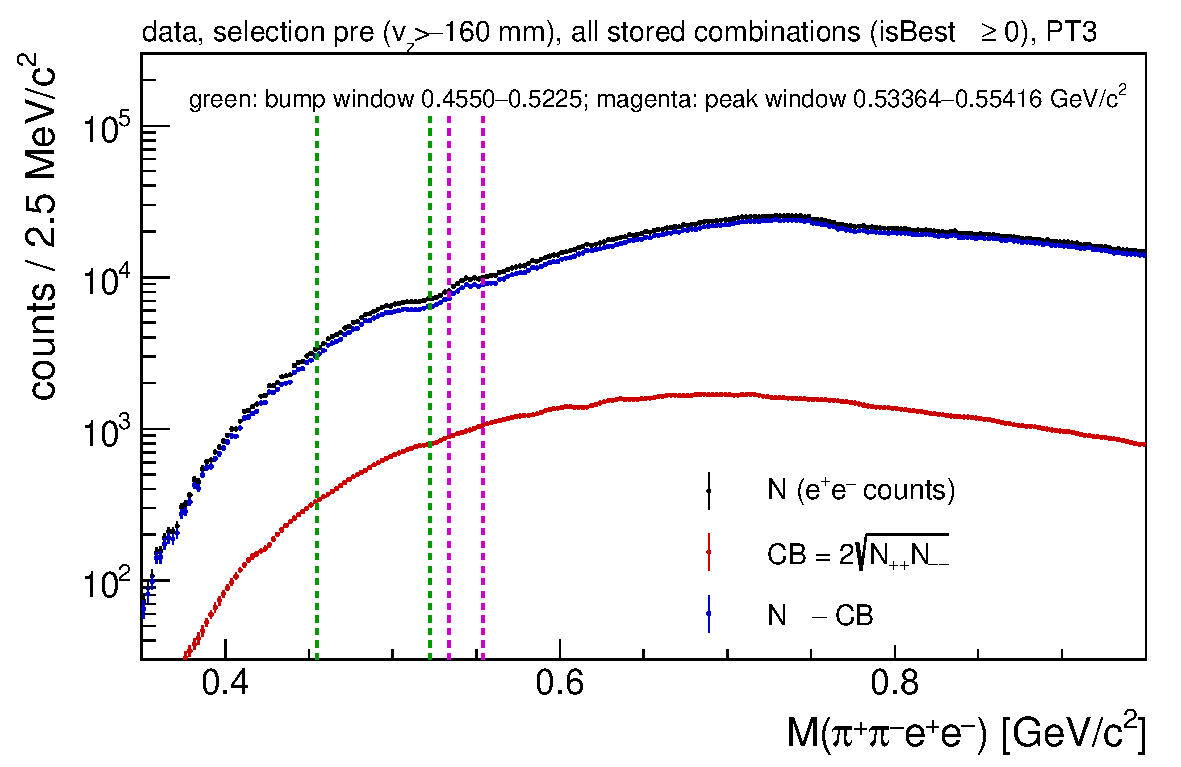
\includegraphics[width=\textwidth]{figs_exp/res_peak_overview_cnt.pdf}
\caption{\Mfour of the data, selection ``pre'' ($\vz>-160$\,mm, PT3, $\vz>-500$\,mm, corrected momenta), all combinations
(isBest $\ge0$). Selection: data with the base cuts \ptthreecap{}, an event vertex reconstructed ($\vz>-500$\,mm) and inside the target region ($\vz>-160$\,mm), particles identified by the START-free velocity \betanew (pions within $3\sigma$, leptons within $5\sigma$ of the expected band; leptons with a RICH ring), energy-loss-corrected momenta for all four tracks, all stored \ppee combinations of each event (isBest $\ge0$), no further cut (together ``pre''); the like-sign counts ($\pipi e^+e^+$, $\pipi e^-e^-$) of the CB pass the same cuts. Black: $N$; red: CB $=2\sqrt{N_{++}N_{--}}$ (10\,\MeVcc bins interpolated, $k=1$); blue: $N-\mathrm{CB}$; 2.5\,\MeVcc bins,
log scale. Green lines: data bump window 0.4550--0.5225\,\GeVcc; magenta lines: data peak window 0.53364--0.55416\,\GeVcc. Counts, not
normalised to luminosity.}
\label{fig:res_overview}
\end{figure}

\begin{figure}[H]
\centering
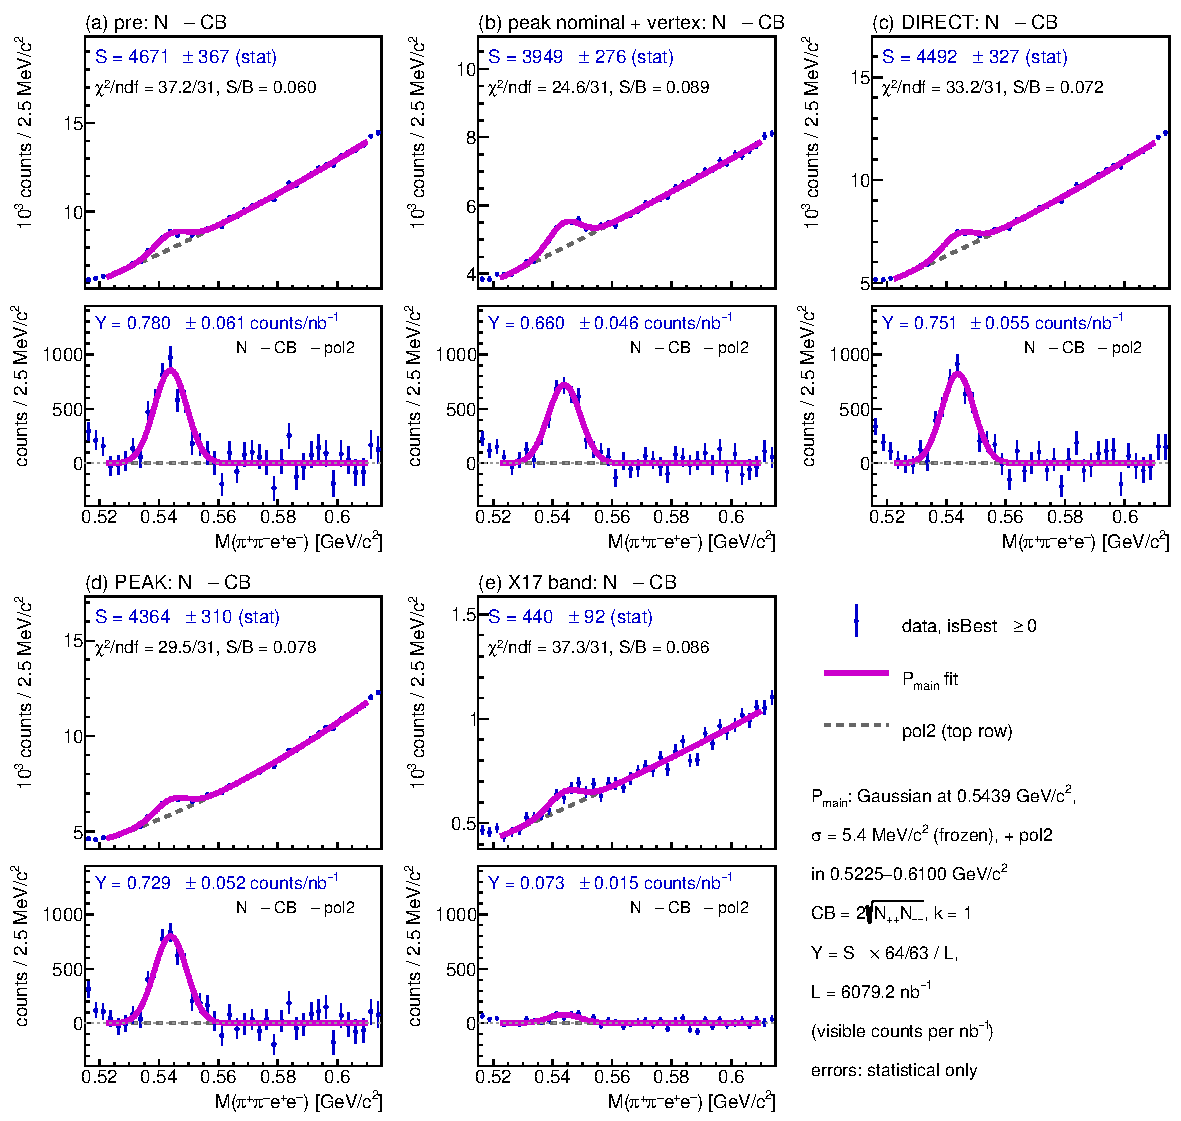
\includegraphics[width=\textwidth]{figs_exp/res_peak_fits_cnt.pdf}
\caption{The $\eta$ peak for the final candidates, all combinations (isBest $\ge0$): (a) ``pre'', (b) peak nominal + vertex, (c)
DIRECT, (d) PEAK, (e) X17 band (``pre'' + $15.5\le\Mee<24.5$\,\MeVcc + both pions in the vertex fit, without its \Mfour window). Selection: data with the base cuts \ptthreecap{}, an event vertex reconstructed ($\vz>-500$\,mm) and inside the target region ($\vz>-160$\,mm), particles identified by the START-free velocity \betanew (pions within $3\sigma$, leptons within $5\sigma$ of the expected band; leptons with a RICH ring), energy-loss-corrected momenta for all four tracks, all stored \ppee combinations of each event (isBest $\ge0$) (together ``pre''); in addition (a) nothing, (b) angle between the \pipi and the \ee momenta in the laboratory $\alab<55^\circ$, $\Mpipi>0.30$\,\GeVcc and both pion tracks used in the fit of the event vertex, (c) both pion tracks within 40\,mm of the event vertex along the beam ($\dzpi<40$\,mm), (d) $\dzpi<40$\,mm and missing mass of \ppee below 2.85\,\GeVcc ($\MMfour<2.85$\,\GeVcc), (e) both pions in the vertex fit and $15.5\le\Mee<24.5$\,\MeVcc, all \Mfour; fit range 0.5225--0.6100\,\GeVcc.
Top: $N-\mathrm{CB}$ in $10^3$ counts per 2.5\,\MeVcc with the \Pmain fit (magenta: frozen Gaussian 0.5439\,\GeVcc, 5.4\,\MeVcc, + pol2 in
0.5225--0.6100) and the pol2 alone (grey dashed); $S\pm$stat, $\chi^2/\mathrm{ndf}$, $S/B$. Bottom: $N-\mathrm{CB}-\mathrm{pol2}$, equal
y ranges; $Y=S\times\frac{64}{63}/L$ with $L=6079.2\,\nbinv$ in visible counts per \nbinv (stat only; luminosity $\pm6.9$\,\% not included).
Last panel: key. The model uncertainty is not printed (Table~\ref{tab:fix_spread}). CB with $k=1$.}
\label{fig:res_fits}
\end{figure}

\subsection{Model uncertainty and statistical errors revisited}
\label{sec:fixmodel}
Two questions of the review are answered here (macro \code{plots/exp_report/fix_checks.C}, all numbers in
\code{tables_exp/fix_checks.txt}; Tables~\ref{tab:fix_spread} and~\ref{tab:fix_stat}, Fig.~\ref{fig:fix_spread}).

\textbf{Model uncertainty of $S$: procedure.} The old envelope of the chapters (\S\ref{sec:proc}) has three of its four fit
ranges starting below the highest bump edge (0.5202\,\GeVcc, smeared by 5.4\,\MeVcc), and its nominal range is not one of the
variations. It is therefore recomputed and compared with an edge-safe version: (1) the old envelope with its rms and the share
of its passing variations below the nominal $S$; (2) an edge-safe grid with every lower bound $\ge0.5225$: order 1--4 $\times$
lower bound 0.5225/0.5250/0.5275 $\times$ upper bound 0.590/0.610/0.630/0.650 $\times$ width $0.0054\pm0.0005$\,\GeVcc (144 fits,
kept if $p>0.05$); (3) the components one at a time, each as the half range over its passing fits with the nominal fit included:
the order alone (pol1--pol4 in the nominal range), the range alone (12 ranges, pol2) and the width alone ($\pm0.5$\,\MeVcc).

\textbf{Result} (PEAK; ``pre'' in brackets). Old envelope 867 (958) from 28 (21) passing fits, rms 498 (545); 71\,\% (67\,\%) of
these fits lie \emph{above} the nominal $S$: once higher orders are allowed, the lower bounds below the edge do not pull $S$ down
(Fig.~\ref{fig:fix_spread}). The edge-safe grid keeps 90 (86) of 144 fits, with half range 958 (958) and rms 477 (453): removing
the ranges that cross the edge does \emph{not} make the envelope smaller. The components are: order 118 (167), range 47 (74),
width 328 (349), quadrature sum 352 (394). The width of the frozen Gaussian ($\pm0.5$\,\MeVcc, about one standard deviation of
the free fit) dominates; the large half ranges come from combinations of a high order with a short range, whose $S$ also scatter
by statistics, and a half range over 90--130 such fits picks the extremes. The nominal value lies in the middle of the edge-safe
variations (40\,\% (47\,\%) of them below it).

\textbf{Decision.} The model uncertainty quoted in the summaries (\S\ref{sec:results}, status box of Appendix~\ref{app:status}, \S\ref{sec:recommend}, Table~\ref{tab:syst}, short
report) is the rms of the edge-safe grid: 8.8--10.9\,\% of $S$ for the six candidate selections and 13.6\,\% for the X17 band
(Table~\ref{tab:fix_spread}); with it $F_{\mathrm{tot}}=7.6$--8.6 instead of 4.0--4.7. The chapter tables and figures still print
the old envelope (half range), which is about twice larger and is kept as a conservative bound. The peak position is not varied in
either (\S\ref{sec:scale}).

% fix_spread_cnt.tex: copy of fix_spread.tex with "rows" -> "counts" (analyst, 15 Nov 2026; Part II writer, integ4)
% written by plots/exp_report/fix_checks.C (review fixes)
\begin{table}[H]\centering\footnotesize\setlength{\tabcolsep}{3pt}
\caption{Model uncertainty of the $\eta$-peak content $S$ (\Pmain), experimental data, all combinations (isBest $\geq0$, top) and isBest $=1$ (bottom), no OA cut. \emph{Old envelope} (chapter tables): half range of $S$ over the 48 variations (order 1--4, four ranges with lower bounds 0.505--0.520\,\GeVcc, width $\pm0.5$\,\MeVcc) with $p>0.05$ ($n$ fits), its rms and the share of these fits below the nominal $S$. \emph{Edge-safe} (every lower bound $\geq0.5225$\,\GeVcc): half range over the fits with $p>0.05$ (nominal included) of the polynomial order alone (pol1--pol4, nominal range), of the range alone (lower bound 0.5225/0.5250/0.5275 $\times$ upper bound 0.590/0.610/0.630/0.650, pol2) and of the width alone ($\pm0.5$\,\MeVcc), their quadrature sum, and the half range and rms of the full grid of 144 combinations ($n$ fits with $p>0.05$). \textbf{Quoted model uncertainty $=$ rms of the edge-safe grid.} stat$_g$ $=$ fit error $\times\sqrt{\mathrm{var}/N}$ (event-group factor of the unlike-sign counts in the data peak window); $F_{\mathrm{tot}}=S/\sqrt{\mathrm{stat}_g^2+\mathrm{model}^2}$. CB with $k=1$; counts, not normalised to luminosity.}
\label{tab:fix_spread}
\resizebox{\textwidth}{!}{%
\begin{tabular}{@{}l r r r | r r r | r r r r r r | r@{}}
\toprule
 & & & & \multicolumn{3}{c|}{old envelope} & \multicolumn{6}{c|}{edge-safe} & \\
selection & $S$ & stat & stat$_g$ & half ($n$) & rms & below & order & range & width & quad.\ & grid half ($n$) & \textbf{model} (rms) & $F_{\mathrm{tot}}$ \\
\midrule
pre & 4671 & 367 & 372 & 958 (21) & 545 & 0.33 & 167 & 74 & 349 & 394 & 958 (86) & \textbf{453} & 7.96 \\
pre + vertex & 4388 & 307 & 310 & 1078 (30) & 547 & 0.37 & 82 & 69 & 330 & 347 & 809 (117) & \textbf{420} & 8.41 \\
peak nominal & 4330 & 327 & 331 & 981 (30) & 509 & 0.40 & 159 & 107 & 316 & 370 & 845 (132) & \textbf{380} & 8.59 \\
peak nominal + vertex & 3949 & 276 & 278 & 936 (31) & 481 & 0.32 & 219 & 73 & 282 & 364 & 883 (132) & \textbf{373} & 8.49 \\
DIRECT & 4492 & 327 & 331 & 907 (21) & 523 & 0.24 & 116 & 55 & 329 & 353 & 773 (114) & \textbf{423} & 8.36 \\
PEAK & 4364 & 310 & 313 & 867 (28) & 498 & 0.29 & 118 & 47 & 328 & 352 & 958 (90) & \textbf{477} & 7.65 \\
X17 band & 440 & 92 & 93 & 133 (27) & 70 & 0.52 & 53 & 70 & 39 & 96 & 147 (117) & \textbf{60} & 3.97 \\
\midrule
\multicolumn{14}{@{}l}{isBest $=1$} \\
pre & 4199 & 330 & 330 & 671 (16) & 447 & 0.31 & 109 & 31 & 323 & 342 & 748 (55) & \textbf{414} & 7.93 \\
pre + vertex & 3966 & 280 & 280 & 955 (28) & 484 & 0.43 & 67 & 72 & 308 & 323 & 850 (116) & \textbf{398} & 8.15 \\
peak nominal & 3895 & 295 & 295 & 776 (32) & 418 & 0.44 & 146 & 78 & 296 & 339 & 671 (126) & \textbf{355} & 8.44 \\
peak nominal + vertex & 3602 & 252 & 252 & 750 (32) & 403 & 0.41 & 195 & 84 & 268 & 342 & 663 (126) & \textbf{341} & 8.49 \\
DIRECT & 4112 & 296 & 296 & 677 (18) & 422 & 0.28 & 88 & 68 & 308 & 328 & 821 (108) & \textbf{391} & 8.39 \\
PEAK & 4061 & 281 & 281 & 782 (26) & 450 & 0.38 & 53 & 28 & 312 & 318 & 957 (85) & \textbf{470} & 7.42 \\
X17 band & 368 & 84 & 84 & 122 (42) & 57 & 0.74 & 67 & 64 & 34 & 99 & 128 (135) & \textbf{59} & 3.57 \\
\bottomrule
\end{tabular}}
\end{table}


\begin{figure}[!htbp]
\centering
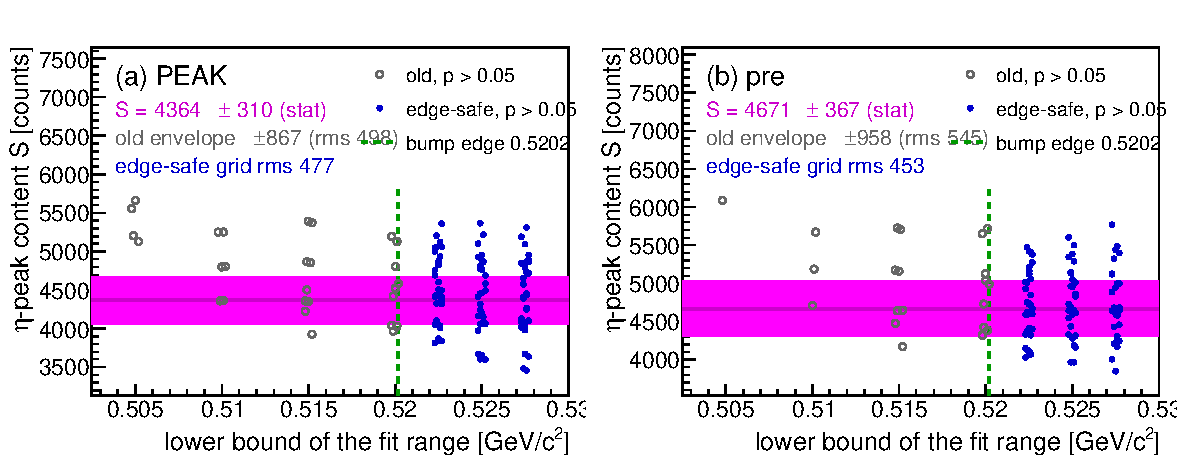
\includegraphics[width=\textwidth]{figs_exp/fix_spread_cnt.pdf}
\caption{$\eta$-peak content $S$ of the \Pmain fit variations against the lower bound of the fit range, data, all combinations
(isBest $\ge0$), (a) PEAK, (b) ``pre''. Selection: data with the base cuts \ptthreecap{}, an event vertex reconstructed ($\vz>-500$\,mm) and inside the target region ($\vz>-160$\,mm), particles identified by the START-free velocity \betanew (pions within $3\sigma$, leptons within $5\sigma$ of the expected band; leptons with a RICH ring), energy-loss-corrected momenta for all four tracks, all stored \ppee combinations of each event (isBest $\ge0$) (together ``pre''); (a) in addition both pion tracks within 40\,mm of the event vertex along the beam ($\dzpi<40$\,mm) and missing mass of \ppee below 2.85\,\GeVcc ($\MMfour<2.85$\,\GeVcc) (PEAK), (b) no further cut. Grey open circles: the 48 old variations (order 1--4, four ranges, width $\pm0.5$\,\MeVcc)
that pass $p>0.05$; blue: the 144 edge-safe variations (lower bound 0.5225/0.5250/0.5275, four upper bounds, order 1--4, width
$\pm0.5$\,\MeVcc) that pass; points of one lower bound are spread slightly in $x$ for visibility. Magenta: nominal $S$ with its
statistical error (band). Green: the highest kinematic edge of the bump, 0.5202\,\GeVcc. CB with $k=1$; counts, not normalised to
luminosity.}
\label{fig:fix_spread}
\end{figure}

\textbf{Statistical errors: procedure.} (1) The event-group factor $\sqrt{\mathrm{var}/N}$ of the unlike-sign counts in the data
peak window is 1.008--1.016 for isBest $\ge0$ and exactly 1 for isBest $=1$ (stat$_g$ in Table~\ref{tab:fix_spread}). (2) The fit
errors are checked on the data with independent halves: for the fold split and for 40 random halvings of the event groups (the
hash of the bias study, \S\ref{sec:bias}) the two halves are fitted alone, and the pull $z=(X_A-X_B)/\sqrt{\sigma_A^2+\sigma_B^2}$ is
formed for $S$ and for $E$. If the errors are right, $\sqrt{\langle z^2\rangle}=1$ within about $\pm0.11$.

\textbf{Result} (Table~\ref{tab:fix_stat}). For $S$, $\sqrt{\langle z^2\rangle}=0.91$--1.02 in five selections: the fit errors of
$S$ are right within the precision of the test, and the event-group term (0.8--1.6\,\%) is below it; no scaling is applied. For
$E$, $\sqrt{\langle z^2\rangle}=1.20$ (``pre'') and 1.17 (bump nominal + vertex), with 4 of 40 halvings beyond $|z|=2$ in each. The first
draft read this as fit errors of $E$ too small by a factor 1.2 and multiplied them by 1.2 where stated (``pre'': $\pm71\to\pm85$). The mean
pulls over the random halvings are compatible with 0 ($E$: $-0.22\pm0.19$).

\textbf{Later check: bootstrap of $E$} (Part~III, package bedge, with an independent verifier). The 40 halvings share events, so their
$\sqrt{\langle z^2\rangle}$ is known only to about $\pm0.11$--0.13. A direct measurement: 200 bootstrap replicas of the data, each event
group with a Poisson(1) weight, the edge-step fit repeated on each. The rms of the replicas over the fit error is 0.978 for ``pre'', 1.036 for
``pre'' + vertex and 1.072 for ``pre'' + vertex with isBest $=1$; the verifier, with own code and seeds, gets 0.99 for ``pre'' + vertex.
\textbf{The fit error of $E$ is right}; the value 1.20 of the halvings was a fluctuation of about 1.5--1.8$\sigma$. This report therefore
quotes $E=1199\pm71\,(\mathrm{stat})\pm287\,(\mathrm{model})$ for ``pre'' (earlier: $\pm85$ with the factor 1.2, not confirmed). Only the vertex
study (\S\ref{sec:vtxeff}) keeps the factor 1.2 on $E$, as a labelled conservative choice (Part~III keeps it there too); without it the
combined $\varepsilon_{\mathrm{vtx}}$ is 0.9934 instead of 0.9937. The table below is left as computed.

% fix_stat_cnt.tex: copy of fix_stat.tex with "rows" -> "counts" (analyst, 15 Nov 2026; Part II writer, integ4)
% written by plots/exp_report/fix_checks.C (review fixes)
\begin{table}[H]\centering\small
\caption{Calibration of the statistical errors on the data with independent halves of the event groups, all combinations (isBest $\geq0$). For each halving both halves are fitted alone; pull $z=(X_A-X_B)/\sqrt{\sigma_A^2+\sigma_B^2}$ with the fit errors as quoted ($S$: \Pmain; $E$: sum of the four edge steps). Fold: parity of the group index; 40 random halvings with the hash of the bias study (seeds 1--40). If the errors are right, $\sqrt{\langle z^2\rangle}=1$ (uncertainty about 0.11). CB with $k=1$; counts.}
\label{tab:fix_stat}
\begin{tabular}{@{}l l r r r r@{}}
\toprule
selection & $X$ & $z$ (fold) & $\langle z\rangle$ (40) & $\sqrt{\langle z^2\rangle}$ (40) & $|z|>2$ \\
\midrule
pre & $S$ & $-1.06$ & $-0.00$ & 0.95 & 0 \\
pre + vertex & $S$ & $-1.79$ & $-0.02$ & 0.96 & 2 \\
peak nominal + vertex & $S$ & $-1.02$ & $-0.02$ & 0.91 & 0 \\
DIRECT & $S$ & $-1.62$ & $-0.05$ & 0.95 & 2 \\
PEAK & $S$ & $-1.26$ & $+0.00$ & 1.02 & 1 \\
pre & $E$ & $-2.35$ & $-0.22$ & 1.20 & 4 \\
bump nominal + vertex & $E$ & $-2.20$ & $-0.23$ & 1.17 & 4 \\
\bottomrule
\end{tabular}
\end{table}


\subsection{Mass scale}
\label{sec:scale}
The frozen peak position (free fit $0.54388\pm0.00049$\,\GeVcc, rounded to 0.5439 in the engine) gives the \Mfour scale
$0.54388/0.547862=0.9927\pm0.0009$ (the rounded position gives 0.99277, a difference of $4\times10^{-5}$). The free fits
(Table~\ref{tab:res_scale}) move by $\pm0.6$\,\MeVcc between selections; for ``pre'' the free position is 0.9\,\MeVcc lower
($0.54296\pm0.00046$, about $2\sigma$), and its $S=4548\pm526$ lies within the errors of the frozen-shape value; the model spread
varies the width but not the position. Per period no shift is seen (``pre'': I $0.54305\pm0.00064$, IIA $0.5428\pm0.0043$,
IIB $0.54217\pm0.00104$, III $0.54309\pm0.00106$\,\GeVcc). K$^0_S\to\pipi$ with a displaced pion crossing point gives the \Mpipi scale
$0.99691\pm0.00036$ (all counts; ``pre'' $0.99706\pm0.00035$): the four-particle scale is 0.4\,\% lower than the pion-pair scale. The
simulated peak sits at 0.5460\,\GeVcc (2.1\,\MeVcc higher; simulation/data K$^0_S$ scale $1.0048\pm0.0007$); this is why the frozen windows
are simulation-centred and why data-only numbers use the data windows. The bump edge fitted free sits at the factor $0.9927\pm0.0013$
(``pre''), the same as the peak ($0.9927\pm0.0009$), \S\ref{sec:bump}.

% res_scale_cnt.tex: copy of res_scale.tex with "rows" -> "counts" (analyst, 15 Nov 2026; Part II writer, integ4)
% res_scale.tex -- written by plots/exp_report/res_peak.C (numbers: tables_exp/res_peak.txt)
\begin{table}[H]
\centering\footnotesize
\setlength{\tabcolsep}{3pt}
\caption{Free fit of the $\eta$ peak (position and width free, $P_\mathrm{main}$, 0.5225--0.6100~GeV/$c^2$, pol2; $S$ error includes the shape), the $M_4$ mass scale $=$ position$/m_\eta$ ($m_\eta=0.547862$~GeV/$c^2$), and the fake peak content $S_\mathrm{fake}$ that each selection makes from a smooth background (pass fraction of mixed combinations: pions of one event, lepton pair of another; relative to pre). Data, isBest $\geq0$. Last rows: K$^0_S\to\pi^+\pi^-$ in $M(\pi^+\pi^-)$ with a displaced pion crossing point ($\Delta z_{\pi\pi}>20$~mm, DOCA $<10$~mm); there the scale column is the $M(\pi^+\pi^-)$ scale $=$ position$/m_{K^0}$.}
\label{tab:res_scale}
\begin{tabular}{lccccc}
\toprule
Selection & position [GeV/$c^2$] & width [MeV/$c^2$] & $S$ (free) & $M_4$ scale & $S_\mathrm{fake}$ \\
\midrule
pre & $0.54296\pm0.00046$ & $5.15\pm0.55$ & $4548\pm526$ & $0.9910\pm0.0008$ & 0 (ref.) \\
pre + vertex & $0.54383\pm0.00043$ & $5.40\pm0.50$ & $4390\pm452$ & $0.9926\pm0.0008$ & $+83\pm27$ \\
peak nominal & $0.54358\pm0.00045$ & $5.16\pm0.53$ & $4180\pm465$ & $0.9922\pm0.0008$ & $+18\pm35$ \\
peak nominal + vertex & $0.54424\pm0.00040$ & $5.05\pm0.46$ & $3760\pm372$ & $0.9934\pm0.0007$ & $+73\pm30$ \\
DIRECT & $0.54349\pm0.00043$ & $5.08\pm0.51$ & $4289\pm462$ & $0.9920\pm0.0008$ & $+40\pm23$ \\
PEAK & $0.54345\pm0.00043$ & $5.27\pm0.51$ & $4287\pm450$ & $0.9920\pm0.0008$ & $+83\pm26$ \\
X17 region & $0.54566\pm0.00150$ & $6.35\pm2.10$ & $531\pm188$ & $0.9960\pm0.0027$ & $+15\pm22$ \\
\midrule
K$^0_S$, all counts (no $v_z$ cut) & $0.49607\pm0.00018$ & $5.76\pm0.19$ & $4023\pm127$ & $0.99691\pm0.00036$ & -- \\
K$^0_S$, pre & $0.49615\pm0.00017$ & $5.55\pm0.19$ & $3707\pm117$ & $0.99706\pm0.00035$ & -- \\
K$^0_S$, pre, isBest $=1$ & $0.49619\pm0.00020$ & $5.75\pm0.21$ & $3107\pm108$ & $0.99715\pm0.00039$ & -- \\
\bottomrule
\end{tabular}
\end{table}


\subsection{The bump: edge steps}
\label{sec:bump}
Table~\ref{tab:res_bump} and Fig.~\ref{fig:res_slices} give the edge steps, Eq.~(\ref{eq:edge}). For ``pre'' (isBest $\ge0$)
$E=1199\pm71\pm287$ counts per 2.5\,\MeVcc (a bootstrap confirms the fit error, \S\ref{sec:fixmodel}; the earlier $\pm85$ with a factor 1.2 is
not confirmed); adding the step improves the fit by $\Delta\chi^2=53$, 89, 160 and 29 in the four
slices. The slice 0.40--0.41 ($14\pm17$) and the control slice above the kinematic limit ($17\pm18$) show no step
($\Delta\chi^2$ 0.7 and 0.9); in all variants the control slices are 0 within $2\sigma$ (the largest $-30\pm15$; in the bump-nominal
variants they are slightly negative, $-15$ to $-30$, a small background-shape effect of the size of the $h$ error).
$E$(bump nominal)$/E$(pre) $=0.902$, $E$(bump nominal + vertex)$/E$(pre) $=0.837$, $E(\text{isBest}=1)/E(\ge0)=0.876$; OA$>2^\circ$ keeps
0.74--0.75 of $E$. With the edge position left free the factor between the true limit and the measured edge is $0.9927\pm0.0013$
(``pre'') and $0.9944\pm0.0012$ (bump nominal + vertex), against $0.9927\pm0.0009$ from the $\eta$ peak: \emph{the edge sits where
$\eta\to\pipi\piz$ with a lost photon puts it}. The like-sign counts show no step in \Mfour (\S\ref{sec:cbnull}; in the distance to the
edge, $u$, the $e^-e^-$ counts do, from lepton pairs of the two \piz photons). $E$ is a visibility measure; the
bump yield needs the simulated bump shape (\S\ref{sec:needsim}). \emph{Later (Part~III, 15 November):} measured against the edge of every count,
$u=\Mfour-\Medge(\Mpipi,\Mee)$, the edges of all slices fall on $u=0$ and the data show one step of $1308\pm62$ counts per 2.5\,\MeVcc (21$\sigma$;
\S\ref{sec:edgeu}). $W=N-\mathrm{CB}$ in the bump window ($137\,676\pm435$ for ``pre'') contains
the bump and the physical background and is not a yield either. For bump nominal + vertex the slice 0.39--0.40 fails the fit-quality
rule: the nominal fit has $\chi^2/\mathrm{ndf}=42.8/22$ ($p=0.005$) and none of its 18 variations has $p>0.05$. Its model spread is
therefore \emph{undefined} (counted as 0), and the model error of $E$(bump nominal + vertex) $=1004\pm51\pm244$ is a lower limit.

% wr_res_bump_cnt.tex: copy of wr_res_bump.tex with "rows" -> "counts" (analyst, 15 Nov 2026; Part II writer, integ4)
% wr_res_bump.tex -- copy of res_bump.tex (written by plots/exp_report/res_bump.C) with the caption sentence on the statistical errors
% updated for report_exp.tex (bootstrap of Part III, 15 Nov 2026); the numbers are unchanged
% res_bump.tex -- written by plots/exp_report/res_bump.C (numbers: tables_exp/res_bump.txt)
\begin{table}[H]
\centering\scriptsize
\setlength{\tabcolsep}{2pt}
\caption{Edge step of the bump ($\eta\to\pi^+\pi^-\pi^0$, $\pi^0\to e^+e^-\gamma$ with the photon lost) in slices of $M(\pi^+\pi^-)$ [GeV/$c^2$], experimental data. $h$ = height of the drop of $N-\mathrm{CB}$ at the predicted kinematic edge (position fixed, smearing 5.4~MeV/$c^2$) in counts per 2.5~MeV/$c^2$; $E=\sum h$ over the first four slices $\pm$ stat $\pm$ model spread; $E$ is a visibility measure, not a yield. 0.40--0.41: not in $E$; 0.42--0.46: control slice above the kinematic limit (edge set at 0.5150, $M_{\pi\pi}$ cut dropped). $W=N-\mathrm{CB}$ in the bump window 0.4550--0.5225~GeV/$c^2$ (bump and physical background). Counts: all stored combinations (isBest $\geq0$) or isBest $=1$, corrected momenta, PT3, vertex $z>-500$~mm, $v_z>-160$~mm; not normalised to luminosity. Edge position fitted free (factor measured/true $M_4$, isBest $\geq0$): pre $0.9927\pm0.0013$, bump nominal + vertex $0.9944\pm0.0012$; from the $\eta$ peak $0.9927\pm0.0009$ ($0.54388/0.547862$). The statistical errors are fit errors; a bootstrap with 200 replicas of the data (Part~III) finds them right (0.98--1.04), so the factor 1.2 suggested by 40 halvings of the data (Table~\ref{tab:fix_stat}) is not confirmed. Bump nominal + vertex, slice 0.39--0.40: the nominal fit has $p=0.005$ and no variation passes $p>0.05$, so its model spread is undefined (counted as 0) and the model error of that $E$ is a lower limit.}
\label{tab:res_bump}
\begin{tabular}{llcrrrrrrr}
\toprule
Selection & isBest & $E\pm$stat$\pm$model & 0.30--0.34 & 0.34--0.37 & 0.37--0.39 & 0.39--0.40 & 0.40--0.41 & 0.42--0.46 & $W$ \\
\midrule
pre ($=$ BUMP) & $\geq0$ & $1199\pm71\pm287$ & $330\pm45$ & $380\pm40$ & $355\pm28$ & $134\pm25$ & $14\pm17$ & $17\pm18$ & $137676\pm435$ \\
bump nominal & $\geq0$ & $1082\pm60\pm326$ & $231\pm33$ & $390\pm35$ & $342\pm26$ & $118\pm24$ & $2\pm17$ & $-22\pm18$ & $94520\pm352$ \\
bump nominal + vertex & $\geq0$ & $1004\pm51\pm244$ & $196\pm28$ & $365\pm29$ & $321\pm22$ & $122\pm21$ & $10\pm15$ & $-15\pm15$ & $73770\pm294$ \\
\addlinespace
pre ($=$ BUMP) & $=1$ & $1050\pm64\pm217$ & $280\pm40$ & $339\pm36$ & $313\pm25$ & $118\pm23$ & $18\pm15$ & $3\pm16$ & $111310\pm374$ \\
bump nominal & $=1$ & $938\pm54\pm257$ & $189\pm30$ & $335\pm31$ & $307\pm24$ & $107\pm22$ & $6\pm15$ & $-27\pm16$ & $77094\pm308$ \\
bump nominal + vertex & $=1$ & $884\pm46\pm247$ & $166\pm26$ & $326\pm27$ & $285\pm20$ & $108\pm19$ & $12\pm13$ & $-19\pm14$ & $61371\pm263$ \\
\midrule
\multicolumn{10}{l}{\emph{with OA$(e^+e^-)>2^\circ$ (not a fixed cut)}} \\
pre ($=$ BUMP) & $\geq0$ & $898\pm64\pm160$ & $258\pm40$ & $293\pm36$ & $261\pm25$ & $86\pm23$ & $-7\pm15$ & $7\pm16$ & $105634\pm392$ \\
bump nominal & $\geq0$ & $812\pm53\pm239$ & $176\pm29$ & $304\pm31$ & $257\pm23$ & $75\pm22$ & $-17\pm15$ & $-26\pm16$ & $71037\pm314$ \\
bump nominal + vertex & $\geq0$ & $746\pm44\pm220$ & $156\pm24$ & $272\pm25$ & $241\pm20$ & $76\pm19$ & $-9\pm13$ & $-20\pm13$ & $55020\pm259$ \\
\addlinespace
pre ($=$ BUMP) & $=1$ & $791\pm57\pm122$ & $218\pm36$ & $268\pm32$ & $228\pm23$ & $78\pm20$ & $-2\pm14$ & $-5\pm15$ & $84920\pm336$ \\
bump nominal & $=1$ & $700\pm48\pm192$ & $139\pm26$ & $261\pm28$ & $230\pm21$ & $70\pm20$ & $-12\pm14$ & $-30\pm15$ & $57704\pm274$ \\
bump nominal + vertex & $=1$ & $659\pm40\pm189$ & $127\pm22$ & $250\pm23$ & $213\pm18$ & $68\pm17$ & $-6\pm12$ & $-22\pm12$ & $45698\pm231$ \\
\bottomrule
\end{tabular}
\end{table}


\begin{figure}[!htbp]
\centering
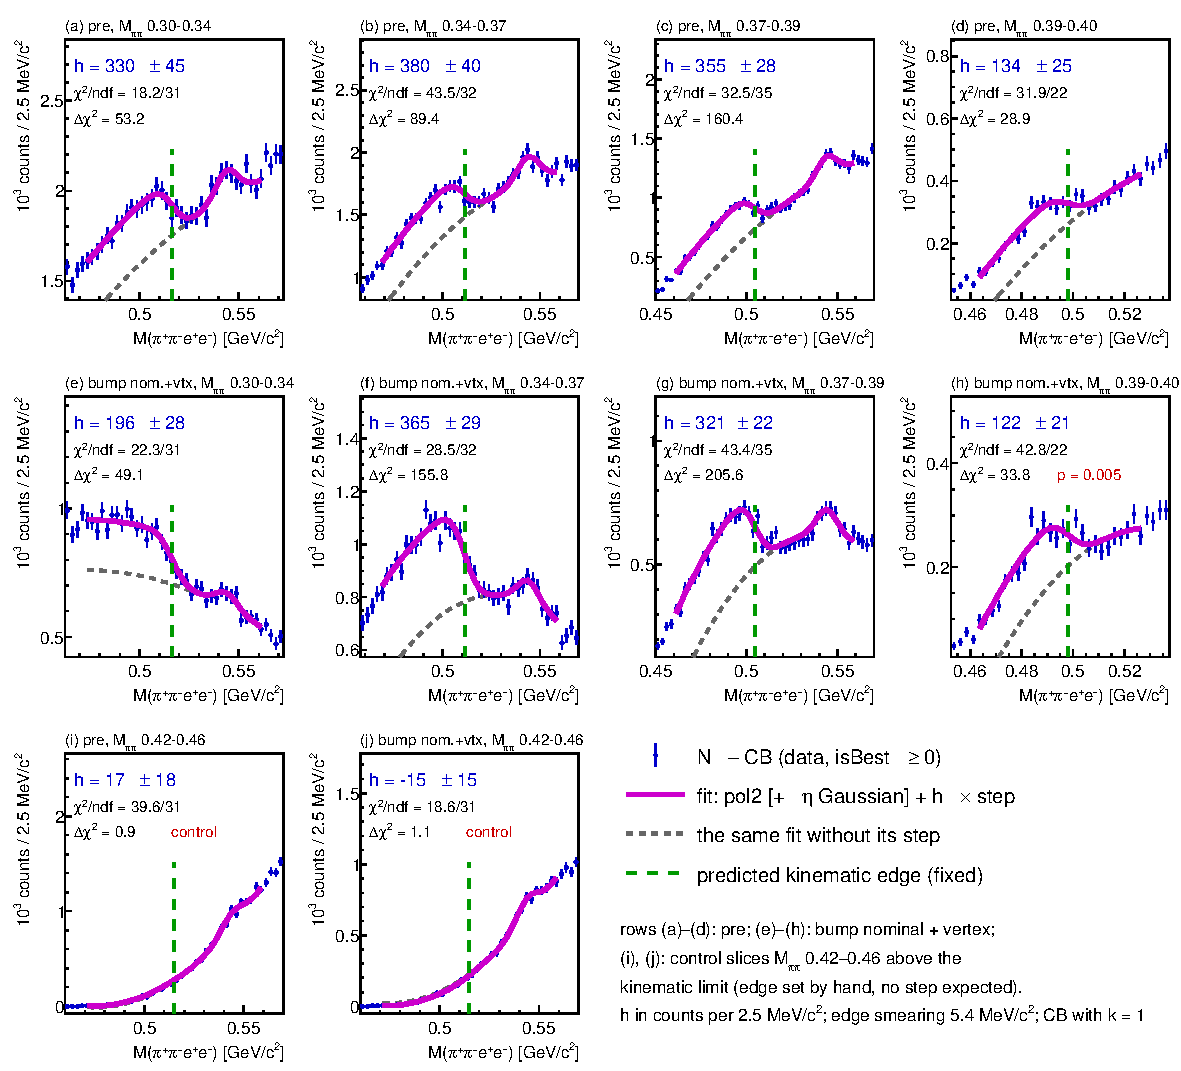
\includegraphics[width=\textwidth]{figs_exp/res_bump_slices_cnt.pdf}
\caption{Edge step of the bump ($\eta\to\pipi\piz$, $\piz\to\ee\gamma$ with the photon lost) in \Mpipi slices [\GeVcc]. Selection: data with the base cuts \ptthreecap{}, an event vertex reconstructed ($\vz>-500$\,mm) and inside the target region ($\vz>-160$\,mm), particles identified by the START-free velocity \betanew (pions within $3\sigma$, leptons within $5\sigma$ of the expected band; leptons with a RICH ring), energy-loss-corrected momenta for all four tracks, all stored \ppee combinations of each event (isBest $\ge0$) (together ``pre''), all \Mee; (a)--(d) no further cut, in the slices $0.30\le\Mpipi<0.34$, 0.34--0.37, 0.37--0.39 and 0.39--0.40\,\GeVcc; (e)--(h) in addition angle between the \pipi and the \ee momenta in the laboratory $\alab<40^\circ$, $0.30<\Mpipi<0.41$\,\GeVcc and both pion tracks used in the fit of the event vertex (bump nominal + vertex), the same slices; (i) ``pre'' and (j) $\alab<40^\circ$ with both pions in the vertex fit (the \Mpipi cut of bump nominal dropped), both in the control slice $0.42\le\Mpipi<0.46$\,\GeVcc. (a)--(d):
``pre'' ($=$ BUMP); (e)--(h): bump nominal + vertex; all combinations (isBest $\ge0$). Blue: $N-\mathrm{CB}$ ($10^3$ counts per 2.5\,\MeVcc,
CB with $k=1$); magenta: fit pol2 [+ $\eta$ Gaussian] + $h\times$ smeared step at the predicted kinematic edge (green dashed; position
fixed, smearing 5.4\,\MeVcc); grey dashed: the fit without its step; $h$ in counts per 2.5\,\MeVcc. (i), (j): control slices 0.42--0.46
above the kinematic limit, edge set by hand, no step expected. (h) fails the fit-quality rule ($p=0.005$). Each panel has its own y range (the slices have very different
background levels). Counts, not normalised to luminosity.}
\label{fig:res_slices}
\end{figure}

\subsection{\texorpdfstring{The bump in the distance to its kinematic edge, $u$ (added on 15 November)}{The bump in the distance to its kinematic edge, u}}
\label{sec:edgeu}
\inshort{Every count has its own edge $\Medge(\Mpipi,\Mee)$; in the distance to it, $u=\Mfour-\Medge$, all edges fall on $u=0$. The data alone show one sharp step there, $h_u=1308\pm62$ counts per 2.5\,\MeVcc (21$\sigma$), $6.3\pm0.7$\,\MeVcc wide; how the tail of the $\eta$ peak is modelled moves it by up to 7\,\% (1217--1308), and the data cannot measure the size of that tail (Part~III takes half of the simulated tail as a systematic term, D40, approved). Like $E$, $h_u$ is not a yield; Part~III turns it into its bump measurement (D37, approved).}
\textbf{Why.} The per-slice measure $E$ (\S\ref{sec:bump}) uses the edge at $\Mee\to0$, Eq.~(\ref{eq:m4max}), and four \Mpipi slices, inside
which the edge moves by 5--7\,\MeVcc. But the edge of a count depends on both measured masses: a heavier \ee pair leaves less energy to the
lost photon and moves the edge up. Part~III (package edgeu, 15 November) therefore measures every count against its own edge.

\textbf{Procedure.} For true masses, the largest \Mfour of $\eta\to\pipi\piz$, $\piz\to\ee\gamma$ with the photon lost is
\begin{equation}
\begin{aligned}
M_4^{\max}(\Mpipi,\Mee)^2&=m_\eta^2-m_\eta\,(E^*-p^*)\left(1-\frac{\Mee^2}{m_{\pi^0}^2}\right),\\
\Medge(\Mpipi,\Mee)&=0.99274\,M_4^{\max}\!\left(\frac{\Mpipi}{0.9970},\Mee\right),\\
u&=\Mfour-\Medge(\Mpipi,\Mee),
\end{aligned}
\label{eq:edgeu}
\end{equation}
with $E^*$, $p^*$ of Eq.~(\ref{eq:m4max}); \Medge is on the measured scale (\Mfour scale 0.99274 of the $\eta$ peak, \Mpipi scale 0.9970 of the
K$^0_S$; the frozen edge function of Part~III), and $u$ is defined for $\Mee<m_{\pi^0}$ (no bump count is lost). This is kinematics only: in
the simulated truth no bump count lies above its edge (Part~III; without the \Mee term 3.8\,\% of the Dalitz counts would). The counts of ``pre'' +
both pions in the vertex fit with $0.30\le\Mpipi<0.40$\,\GeVcc are filled into 2.5\,\MeVcc bins of $u$; the CB is $2\sqrt{N_{++}N_{--}}$ in
10\,\MeVcc cells of $u$, interpolated, per \Mpipi slice (0.30--0.34--0.37--0.39--0.40), as in \S\ref{sec:proc}. $N-\mathrm{CB}$ is fitted on
$-45\le u<+45$\,\MeVcc with
\begin{equation}
N-\mathrm{CB}=\mathrm{pol2}(u)\;[+\,\text{peak term}]+h_u\;\tfrac12\,\mathrm{erfc}\!\left(\frac{u}{\sqrt2\,\sigma_u}\right)\quad\text{(bin averaged)},
\label{eq:edgeufit}
\end{equation}
covariance $=$ cov(CB) $+$ the model of $N$, iterated (the logic of the per-slice fit). $\sigma_u=6.7$\,\MeVcc is the template width of
Part~III (from the simulated resolution at the edge); here it is also left free. The $\eta$ peak enters the range above $u\approx+15$\,\MeVcc,
so three peak treatments are compared: none (the polynomial absorbs the rise), a peak term built from the data (the frozen data Gaussian,
0.5439\,\GeVcc and 5.4\,\MeVcc, placed in $u$ with the measured \Mpipi and \Mee of the peak-window counts minus 0.921 times the side-band counts,
amplitude free), and, for comparison only, the simulated peak shape of Part~III (scaled by the measured peak scale 0.418). Macro
\code{plots/all_report/edgeu_partII_datastep.py} (numbers in \fpath{/hdd3/przygoda/HADES/FAT_out/all_report/edgeu_partII/edgeu_partII.log});
it reproduces the Part~III fit exactly (1305.2).

\begin{table}[H]
\centering
\caption{\textbf{Step at $u=0$ in the data}, ``pre'' + vertex, $0.30\le\Mpipi<0.40$\,\GeVcc, isBest $\ge0$, counts per 2.5\,\MeVcc. Fit range
$-45\le u<+45$\,\MeVcc, pol2, $\sigma_u=6.7$\,\MeVcc unless stated; $\Delta\chi^2$: without the step. Last column: $h_u$ for the fit
ranges $\pm35$, $\pm40$, $\pm50$, $\pm55$ and $-45$\dots$+30$\,\MeVcc (fits with $p<0.05$ in brackets).}
\label{tab:edgeu}
\footnotesize
\begin{tabularx}{\textwidth}{@{}>{\raggedright\arraybackslash}p{4.4cm} c c c L@{}}
\toprule
peak treatment & $h_u$ & $\chi^2/\mathrm{ndf}$ & $\Delta\chi^2$ & other ranges \\
\midrule
none (data only, shown in Fig.~\ref{fig:res-edgeu}) & $1308\pm62$ & 40.2/32 & 439 & 1477, 1408, (1242), (1151), 1472 \\
none, $\sigma_u$ free ($6.3\pm0.7$\,\MeVcc) & $1271\pm85$ & 39.9/31 & 439 & \\
Gaussian from the data, amplitude free & $1217\pm66$ & 24.6/31 & 337 & 1037, 1235, 1232, 1206, 1193 \\
the same, $\sigma_u$ free ($6.5\pm0.8$\,\MeVcc) & $1204\pm91$ & 24.5/30 & & \\
simulated shape $\times$ 0.418 (Part~III, comparison) & $1305\pm62$ & 27.3/32 & 439 & 1353, 1330, 1312, 1284, 1345 \\
the same, $\sigma_u$ free ($7.0\pm0.8$\,\MeVcc) & $1331\pm95$ & & & \\
\bottomrule
\end{tabularx}
\end{table}

\textbf{Results} (Table~\ref{tab:edgeu}, Fig.~\ref{fig:res-edgeu}). \textbf{The step.} Without any simulated input the data show a step at
$u=0$ of $h_u=1308\pm62$ counts per 2.5\,\MeVcc; the fit without it is worse by $\Delta\chi^2=439$ (21$\sigma$). 200 bootstrap replicas of
the data (event groups) give an rms of 63 counts, 1.01 times the fit error. Left free, the step is $6.3\pm0.7$\,\MeVcc wide (Part~III, with
the simulated peak term: $7.0\pm0.8$), the size expected from the mass resolution (the $\eta$ peak has 5.4\,\MeVcc; the template width
from the simulated resolution at the edge, a Gaussian fit on $\pm40$\,\MeVcc, is 6.7\,\MeVcc). \textbf{The peak tail.} Without a peak term the fit is acceptable ($p=0.15$), but the height moves
with the range (1151--1477; the $\pm50$ and $\pm55$\,\MeVcc fits fail), because a second-order polynomial cannot follow both the bump slope and the rise
into the peak. The Gaussian peak term from the data makes the fit better ($\chi^2/\mathrm{ndf}=24.6/31$) and stable against the range
(1205--1235 for $\pm40$ to $\pm55$\,\MeVcc), but 7\,\% lower; its fitted amplitude, $2838\pm717$ counts, agrees with the side-band number of the
peak counts (2740). The simulated peak shape of Part~III has, in addition, a low-mass tail that reaches $u\approx0$; with it the height is
$1305\pm62$ and stable (1284--1353). So the data alone fix the height to within about 7\,\%, and the difference is the modelling of the
low-mass tail of the peak. \textbf{Comparison with $E$.} $E$ sums four slice steps on ``pre'' with the edge at $\Mee\to0$ and a 5.4\,\MeVcc
smearing ($1199\pm71$); on the same counts as here Part~III's per-slice steps sum to 1142, and the $u$ steps per slice to 1295 (13\,\% more),
because in $u$ the step is sharper and the template is wider. Step heights of different estimators are not comparable; only the ratio to the
simulation with the same estimator is (Part~III). \textbf{Checks} (Part~III, data side): the four \Mpipi slices give 325, 437, 387 and
145 counts; a control region without bump ($0.42\le\Mpipi<0.46$\,\GeVcc with a pseudo edge $\Medge(\Mpipi-0.10,\Mee)$) gives $3.1\pm16.7$; the
like-sign counts: $e^+e^+$ $2.1\pm6.5$, $e^-e^-$ a step of $73.5\pm15.7$ counts from lepton pairs of the two \piz photons (\S\ref{sec:cbnull}), of
which 39 counts (3\,\% of $h_u$) enter the subtracted CB, as they should.

\textbf{What it means.} The data show the edge of $\eta\to\pipi\piz$, $\piz\to\ee\gamma$ with the lost photon as one sharp step exactly where
the kinematics of every count puts it, at 18--21$\sigma$ whatever the peak treatment. Like $E$, $h_u$ measures how visible the edge is and is
not a yield. \textbf{Later (Part~III, data + simulation):} applied in the same way to the simulated bump, the step gives the $\eta$ scale
$f_\eta(u\text{-edge})=0.426\pm0.020\,(\mathrm{stat})\pm0.034\,(\mathrm{syst})\pm0.030\,(\mathrm{MC})$ of SMASH (per-slice edge 0.423;
both with the per-count QED weights of the C2 decay angle, D38; the systematic error includes the peak-tail term of D40), a visible bump yield of
$21\,468\pm1003\pm1708\pm1347$ counts in the bump window; it is the bump measurement of Part~III (D37, approved by the analyst on
15 November 2026; the per-slice edge is the cross-check). \emph{Status:} measured (the data side of package edgeu, confirmed by an independent verifier); the
data-only fits of this subsection are new and use the same code.

\textbf{Later (Part~III, evening of 15 November): how large is the low-mass tail of the $\eta$ peak in the data?} \emph{In short: the
tail of the simulated peak is the radiation of the leptons in the detector material; the data cannot measure its size, so the 7\,\% between
the two peak treatments stay a modelling question; Part~III keeps the simulated tail and takes a systematic term for it (D40, approved).}
Part~III (package peaktail; the origin of the tail and its effect were confirmed by an independent verifier, package vpt) found in the
simulation that the generated \Mfour of the $\eta$ is a sharp line and that about a quarter of the simulated peak entries lose more than
5\,\MeVcc because the leptons lose momentum in the material; these entries reach $u\approx0$. \emph{Why the two peak terms of
Table~\ref{tab:edgeu} differ} (verifier, same fit): a Gaussian placed at the positions of the \emph{simulated} peak entries gives $h_u=1256$, so
49 of the 88 counts between 1305 and 1217 come from leaving the tail out; the other 39 come from the positions of the peak counts, which
the side-band subtraction of the data puts on average 1.0\,\MeVcc further from their edges than in the simulation (not understood). \emph{How large the tail is in the data:} scaling the simulated tail by a factor $t$ ($t=1$ SMASH, $t=0$
no tail) and fitting $u$ with the peak scale constrained by the peak side bands gives $t=0.0\pm0.9$ to $0.6\pm1.0$, depending on how the 180
simulated entries of $\eta\to\pipi\gamma$ with a converted photon are treated: $t=0.3\pm1.0$. The line shape of the peak where no bump exists
($0.42\le\Mpipi<0.46$\,\GeVcc) cannot tell the tail from a shift of the peak by 1\,\MeVcc. So the data allow both the simulated tail and
no tail; a peak without a tail is excluded by physics (the material exists, and the decay itself radiates, which the generator leaves out),
not by these data (the study's first value, $t=0.72\pm0.38$, is not confirmed). \emph{Meaning:} $h_u$ of this report does not change; Part~III keeps the simulated tail ($t=1$) and takes half of it as a
systematic term, $\pm3.4$\,\% on its bump scale $f_\eta(u\text{-edge})$ (D40, approved by the analyst on 15 November 2026, option (a); no tail
at all would lower it by 6.9\,\%).

\subsection{The ECAL-tagged \texorpdfstring{$\eta$}{eta} as a reference}
\label{sec:tagged}
The tagged sample sees the same decay as the bump with the photon found (Table~\ref{tab:res_tagged}, Fig.~\ref{fig:res_tagged}).
For ``pre'' $T=3314\pm105\pm124$ ($S/B=0.73$, $T/\mathrm{err}=31.6$; free position $0.5463\pm0.0002$\,\GeVcc, width $6.19\pm0.24$\,\MeVcc),
$Y_T=0.554\pm0.018$ visible counts per \nbinv. The cuts keep 0.910 (bump nominal), 0.851 (bump nominal + vertex) and 0.860 (isBest $=1$) of $T$; OA$>2^\circ$ keeps
$2506/3314$. Almost all tagged $\eta$ lie in the bump window, as the kinematics demand (the share from two separate fits, 0.94, is
uncertain by about 0.1). \textbf{Photon energy.} The \piz of the tagged $\eta$ sits at $M(\ee\gamma)=0.1460\pm0.0005$\,\GeVcc (width
$13.7\pm0.5$\,\MeVcc), 8\,\% above $m_{\pi^0}$; the photon energy itself is about 17\,\% too high (median rescaling factor 0.856).
The ECAL energy is not calibrated; $m_{5c}$ corrects this combination by combination, so $T$ is not affected. The 100\,MeV cut on the cluster energy
therefore acts near 85\,MeV of true photon energy ($100\times0.856$); in the simulation, whose cluster energy is 7--9\,\% low, the same cut
acts near 108\,MeV (Part~III). With all \ee counts that have a good photon the \piz sits at 141.9\,\MeVcc (width 14.3\,\MeVcc; Part~III).

\textbf{ECAL status in the data} (later, Part~III; data side). The ECAL has six sectors of 163 modules. In the data parameter file (first
runs of the days 034, 039, 045, 047, 049, 053, 059 and 067, all four periods) \textbf{ECAL sector~0} (azimuth 63--117$^\circ$; not the tracking
sector~2 of the trigger deficit, which lies at 180--240$^\circ$) is switched off, and 8 further modules are dead: 807 of the 978 modules are
active, with the same map at every run and the same map as in the simulation. Seen from the target centre ($z\approx-124$\,mm) the module
corners span 10.9--45.6$^\circ$ in polar angle. The tagged photons of the data agree in azimuth and polar angle with the simulated ones and
leave ECAL sector~0 empty. The acceptance of the tag is therefore known; its photon energy scale and the module efficiency are not.
Part~III's own pass over the entries reproduces $T(\text{``pre''})=3314\pm105$ exactly and gives $T=3090\pm94$ for ``pre'' + vertex (its base S0).

\textbf{START and the photon cut} (later, Part~III; data only). The photon cut $0.8<\beta<1.2$ uses the START time. The 6.4\,\% of the \ee counts
without a START hit (7.2\,\% in the bump window) are tagged at only $0.80\pm0.12$ (all \Mfour) or $0.69\pm0.11$ (bump window) of the normal
rate: $T=3145\pm102$ with START and $170\pm26$ without. The tag therefore loses 1.4\,\% (share of the counts without START over all \Mfour) to
2.3\,\% (share in the bump window) of $T$. The simulation always has a START hit, so a simulated tag does not have this loss; $T$ itself is
quoted as measured.

\textbf{Peak over tagged.} $S/T=1.409\pm0.119\,(\mathrm{stat})\pm0.294\,(\mathrm{model})$ for ``pre'' (model from the old envelope of $S$;
with the revised model uncertainty of $S$, $\pm0.15$) (isBest $=1$: $1.474\pm0.126\pm0.243$;
OA$>2^\circ$: $1.449\pm0.142\pm0.306$), uncorrected for the different acceptances; the two fits are treated as independent although 29\,\%
of the tagged counts in the $m_{5c}$ range are also in the \Pmain \Mfour range.

% res_tagged_cnt.tex: copy of res_tagged.tex with "rows" -> "counts" (analyst, 15 Nov 2026; Part II writer, integ4)
% res_tagged.tex -- written by plots/exp_report/res_bump.C (numbers: tables_exp/res_bump.txt)
\begin{table}[H]
\centering\small
\setlength{\tabcolsep}{4pt}
\caption{ECAL-tagged $\eta$ (reference sample of the bump): counts with an ECAL photon and $0.119\leq M(e^+e^-\gamma)<0.173$~GeV/$c^2$, $m_{ee}<0.10$~GeV/$c^2$; $m_{5c}=M(\pi^+\pi^-e^+e^-\gamma)$ with the photon energy rescaled so that $M(e^+e^-\gamma)=m_{\pi^0}$. $T$ = content of the frozen Gaussian (0.5463~GeV/$c^2$, 6.2~MeV/$c^2$) + pol2 fit of $N-\mathrm{CB}$ in 0.49--0.62 $\pm$ stat $\pm$ model spread; $S/B$ in $\pm1.9\sigma$; width from the free fit. $Y_T=T\times\frac{64}{63}/L$ in visible counts per nb$^{-1}$, $L=6079.2$~nb$^{-1}$ (uncorrected; luminosity uncertainty $\pm6.9$\% not included). $\pi^0$ of the tagged $\eta$ in $M(e^+e^-\gamma)$: $0.1460\pm0.0005$~GeV/$c^2$, $\sigma=13.7\pm0.5$~MeV/$c^2$ (photon energy not calibrated).}
\label{tab:res_tagged}
\begin{tabular}{llcccc}
\toprule
Selection & isBest & $T\pm$stat$\pm$model & $S/B$ & width [MeV/$c^2$] & $Y_T$ [counts/nb$^{-1}$] \\
\midrule
pre ($=$ BUMP) & $\geq0$ & $3314\pm105\pm124$ & 0.73 & $6.2\pm0.2$ & $0.554\pm0.018$ \\
bump nominal & $\geq0$ & $3014\pm93\pm132$ & 0.91 & $6.2\pm0.2$ & $0.504\pm0.016$ \\
bump nominal + vertex & $\geq0$ & $2820\pm84\pm91$ & 1.12 & $5.9\pm0.2$ & $0.471\pm0.014$ \\
pre ($=$ BUMP) & $=1$ & $2850\pm96\pm116$ & 0.76 & $6.3\pm0.3$ & $0.476\pm0.016$ \\
bump nominal & $=1$ & $2593\pm85\pm122$ & 0.94 & $6.2\pm0.3$ & $0.433\pm0.014$ \\
bump nominal + vertex & $=1$ & $2448\pm78\pm98$ & 1.16 & $5.9\pm0.2$ & $0.409\pm0.013$ \\
\midrule
\multicolumn{6}{l}{\emph{with OA$(e^+e^-)>2^\circ$}} \\
pre ($=$ BUMP) & $\geq0$ & $2506\pm93\pm98$ & 0.70 & $6.3\pm0.3$ & $0.419\pm0.015$ \\
bump nominal & $\geq0$ & $2255\pm81\pm105$ & 0.88 & $6.2\pm0.3$ & $0.377\pm0.014$ \\
bump nominal + vertex & $\geq0$ & $2117\pm73\pm83$ & 1.11 & $5.8\pm0.3$ & $0.354\pm0.012$ \\
pre ($=$ BUMP) & $=1$ & $2182\pm85\pm95$ & 0.75 & $6.4\pm0.3$ & $0.365\pm0.014$ \\
bump nominal & $=1$ & $1959\pm75\pm96$ & 0.93 & $6.3\pm0.3$ & $0.327\pm0.012$ \\
bump nominal + vertex & $=1$ & $1856\pm68\pm77$ & 1.16 & $5.9\pm0.3$ & $0.310\pm0.011$ \\
\bottomrule
\end{tabular}
\end{table}


\begin{figure}[!htbp]
\centering
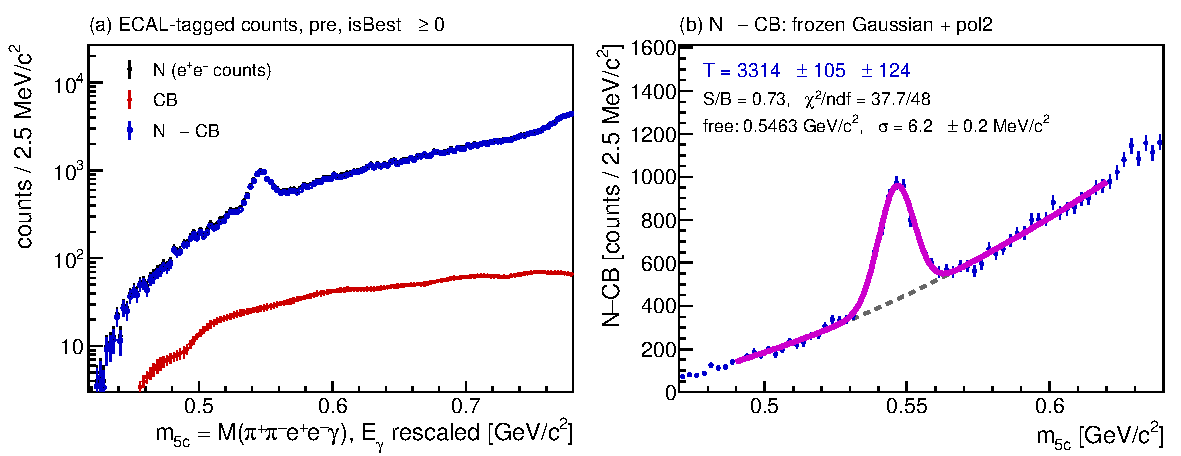
\includegraphics[width=\textwidth]{figs_exp/res_bump_tagged_cnt.pdf}
\caption{ECAL-tagged $\eta$, data, selection ``pre'', all combinations (isBest $\ge0$): counts with an ECAL photon,
$0.119\le M(\ee\gamma)<0.173$\,\GeVcc, $\Mee<0.10$\,\GeVcc; x axis $m_{5c}=M(\ppee\gamma)$ with the photon energy rescaled so that
$M(\ee\gamma)=m_{\pi^0}$. Selection: data with the base cuts \ptthreecap{}, an event vertex reconstructed ($\vz>-500$\,mm) and inside the target region ($\vz>-160$\,mm), particles identified by the START-free velocity \betanew (pions within $3\sigma$, leptons within $5\sigma$ of the expected band; leptons with a RICH ring), energy-loss-corrected momenta for all four tracks, all stored \ppee combinations of each event (isBest $\ge0$) (together ``pre''); an ECAL photon identified as a photon with $0.8<\beta<1.2$ and energy above 100\,MeV (of up to three such photons the one with $M(\ee\gamma)$ closest to 0.140\,\GeVcc), $0.119\le M(\ee\gamma)<0.173$\,\GeVcc and $\Mee<0.10$\,\GeVcc; fit range $0.49\le m_{5c}<0.62$\,\GeVcc. (a) $N$ black, CB red (20\,\MeVcc bins interpolated, $k=1$), $N-\mathrm{CB}$ blue open; log scale. (b) $N-\mathrm{CB}$ with the
frozen Gaussian (0.5463\,\GeVcc, 6.2\,\MeVcc) + pol2 fit in 0.49--0.62; $T$ = Gaussian content $\pm$stat$\pm$model; free position and
width given. Counts, not normalised to luminosity.}
\label{fig:res_tagged}
\end{figure}

\subsection{\texorpdfstring{Content of the peak against $M(e^+e^-)$ and OA}{Content of the peak against M(ee) and OA}}
\label{sec:mee}
The $\eta$-peak content was split into classes of \Mee and of OA with the side-band method, Eq.~(\ref{eq:sb}); the CB of each class
comes from the like-sign counts of the same class (Table~\ref{tab:res_mee}, Fig.~\ref{fig:res_mee}). The side-band contents
$S_{\mathrm{SB}}$ of the classes add up to $4798\pm440$ against $4784\pm440$ for the whole selection with the same method and
$4671\pm367$ from \Pmain. A \Pmain fit of each class alone agrees within the errors.

\textbf{Share above 20\,\MeVcc.} 0.234$\pm$0.043$\pm$0.002 (side band) against $0.280\pm0.036$ (per-class fits) for ``pre''; similar for
isBest $=1$ (0.233), peak nominal (0.225) and peak nominal + vertex (0.255). On the definition of the earlier estimate ($\alab<55^\circ$,
$\Mpipi>0.30$, no $\vz$ cut) the per-class fits reproduce the earlier $0.306\pm0.038$, the side-band method gives 0.05--0.06 less. The two
methods use different \Mfour information (side bands $\pm11$\,\MeVcc, fits 0.5225--0.61); their difference, 1.2--1.5$\sigma$, is a method
systematic. \textbf{Side-band test.} For pairs with $\Mee>0$ the bump edge lies above $M_4^{\max}$ (\S\ref{sec:proc}): at
$\Mee=50$--100\,\MeVcc and \Mpipi near threshold it reaches 0.524--0.533\,\GeVcc, inside the lower side band, which could make
$D$ too small in the high-\Mee classes. The share was therefore recomputed (\code{fix_checks.txt}, part D) with the upper side band
only ($0.232\pm0.049$), the lower only ($0.237\pm0.056$) and an upper band of double width ($0.217\pm0.042$), and on the base
``pre'' + $\Mpipi>0.33$\,\GeVcc, where the bump edge stays below the lower side band for every \Mee (both side bands 0.234, upper only
0.241, per-class fits 0.267). The side-band share does not depend on the side bands; the bump edge does not bias it. The difference
to the per-class fits remains a method systematic. \textbf{Quoted: $0.23\pm0.04\,(\mathrm{stat})\pm0.05\,(\mathrm{method})$} for
``pre'' (mean of the two methods 0.26). $r_{SB}$ of each class changes the share by at
most $+0.013$, CB$\times1.03$ by less than 0.001; the statistical error of $r_{SB}$ is not propagated (a shift of 0.0016 moves the class
contents by 2--3\,\% but the share by 0.001). OA$>2^\circ$ share $0.772\pm0.037$ (the \Pmain ratio gives 0.778); content on one RICH ring
$0.439\pm0.045$.

\textbf{Plain reading.} Below 10\,\MeVcc and below $2^\circ$ most of the $\eta$ content sits on one shared RICH ring (0.92 in 0--5\,\MeVcc, 0.65
in 5--10\,\MeVcc, 0.97 in 0--$1^\circ$ and 0.90 in 1--$2^\circ$); above 20\,\MeVcc and above $6^\circ$ none does. Ring sharing follows the
opening angle: any pair with a few degrees of OA, from a direct decay as well as from a conversion, shares a ring, so it does \emph{not}
tell the two origins apart. The only data-side hint is the \Mee shape: a direct decay alone (Kroll--Wada, roughly $1/\Mee$: equal content
per logarithmic interval before acceptance) would put about $650\times\ln2/\ln2.5\approx490$ counts into each of the bins 5--10 and
10--20\,\MeVcc, where 650 is the content of the 20--50\,\MeVcc class (Table~\ref{tab:res_mee}), assumed to be pure direct decay with the
same acceptance. The data hold 1673 and 1236, an excess of about $1900\pm400$ counts (about 40\,\% of the peak) in 5--20\,\MeVcc, which
would fit $\eta\to\pipi\gamma$ with the photon converted in the material. The data alone do not prove it: the estimate assumes equal
acceptance for close pairs and pairs above 20\,\MeVcc, which only the simulation gives; the class errors are treated as independent
although counts of one event can fall into different classes.

% res_mee.tex -- written by plots/exp_report/res_mee.C (numbers: tables_exp/res_mee.txt)
\begin{table}[H]
\centering\footnotesize
\setlength{\tabcolsep}{3pt}
\caption{Content of the $\eta$ peak in classes of $M(e^+e^-)$ and OA$(e^+e^-)$, experimental data only. Side-band subtraction in $M_4$: $S_\mathrm{SB}=[(N-\mathrm{CB})_{R_\mathrm{pk}}-r\,(N-\mathrm{CB})_{R_\mathrm{SB}}]/(f_\mathrm{pk}-r f_{SB})$ with the data peak window $R_\mathrm{pk}$ = 0.53364--0.55416, side bands $R_\mathrm{SB}$ = 0.5225--0.53364 and 0.55416--0.56530~GeV/$c^2$, $r$ from the $P_\mathrm{main}$ pol2 of the whole selection; CB $=2\sqrt{N_{++}N_{--}}$ of the class ($k=1$). Errors: statistical (event groups) $\pm$ model ($r$ from pol1/pol3). Ring: share of the class content with both leptons on one RICH ring (it follows the opening angle and does not separate direct decays from conversions). $S_\mathrm{fit}$: $P_\mathrm{main}$ fit of the class alone. Selection pre, all stored combinations (isBest $\geq0$); not normalised to luminosity.}
\label{tab:res_mee}
\begin{tabular}{lrrcccc}
\toprule
Class & $N_\mathrm{pk}$ & CB$/N_\mathrm{pk}$ & $S_\mathrm{SB}\pm$stat$\pm$model & share & ring share & $S_\mathrm{fit}$ \\
\midrule
$M_{ee}$ 0-5 MeV/$c^2$ & 11455 & 0.012 & $768\pm165\pm49$ & $0.160\pm0.032$ & $0.92\pm0.08$ & $718\pm136$ \\
$M_{ee}$ 5-10 MeV/$c^2$ & 26475 & 0.011 & $1673\pm251\pm114$ & $0.349\pm0.043$ & $0.65\pm0.07$ & $1591\pm207$ \\
$M_{ee}$ 10-20 MeV/$c^2$ & 18757 & 0.024 & $1236\pm213\pm79$ & $0.258\pm0.039$ & $0.26\pm0.08$ & $1070\pm175$ \\
$M_{ee}$ 20-50 MeV/$c^2$ & 10597 & 0.108 & $650\pm163\pm41$ & $0.136\pm0.032$ & $-0.04\pm0.02$ & $751\pm137$ \\
$M_{ee}$ 50-100 MeV/$c^2$ & 6798 & 0.437 & $391\pm142\pm16$ & $0.081\pm0.028$ & $0.00\pm0.00$ & $397\pm121$ \\
$M_{ee}$ 100-270 MeV/$c^2$ & 3431 & 0.800 & $81\pm108\pm3$ & $0.017\pm0.022$ & $0.00\pm0.00$ & $169\pm94$ \\
\midrule
OA 0-1$^\circ$ & 3847 & 0.010 & $303\pm95\pm16$ & $0.063\pm0.019$ & $0.97\pm0.09$ & $241\pm78$ \\
OA 1-2$^\circ$ & 12731 & 0.008 & $796\pm174\pm55$ & $0.165\pm0.033$ & $0.90\pm0.08$ & $798\pm143$ \\
OA 2-4$^\circ$ & 27153 & 0.010 & $1680\pm254\pm117$ & $0.349\pm0.043$ & $0.56\pm0.07$ & $1707\pm210$ \\
OA 4-6$^\circ$ & 10509 & 0.019 & $829\pm158\pm44$ & $0.172\pm0.031$ & $0.16\pm0.09$ & $667\pm131$ \\
OA 6-10$^\circ$ & 6956 & 0.047 & $354\pm131\pm29$ & $0.073\pm0.026$ & $0.09\pm0.07$ & $365\pm109$ \\
OA 10-20$^\circ$ & 6880 & 0.151 & $503\pm133\pm25$ & $0.104\pm0.026$ & $-0.00\pm0.00$ & $553\pm112$ \\
OA >20$^\circ$ & 9437 & 0.610 & $353\pm173\pm15$ & $0.073\pm0.034$ & $0.00\pm0.00$ & $374\pm149$ \\
\midrule
\multicolumn{7}{p{0.93\textwidth}}{Share of the content with $M_{ee}>20$~MeV/$c^2$ (stat $\pm$ model; in brackets: per-class fits, and with $r$ of each class):} \\
\multicolumn{7}{p{0.93\textwidth}}{\quad pre: $0.234\pm0.043\pm0.002$ ($0.280\pm0.036$; own $r$: 0.236); OA$>2^\circ$ share $0.772\pm0.037$; shared ring $0.439\pm0.045$} \\
\multicolumn{7}{p{0.93\textwidth}}{\quad pre, isBest $=1$: $0.233\pm0.042\pm0.003$ ($0.270\pm0.036$; own $r$: 0.238); OA$>2^\circ$ share $0.766\pm0.037$; shared ring $0.459\pm0.045$} \\
\multicolumn{7}{p{0.93\textwidth}}{\quad peak nominal: $0.225\pm0.043\pm0.001$ ($0.284\pm0.035$; own $r$: 0.237); OA$>2^\circ$ share $0.770\pm0.038$; shared ring $0.451\pm0.046$} \\
\multicolumn{7}{p{0.93\textwidth}}{\quad peak nominal + vertex: $0.255\pm0.037\pm0.002$ ($0.290\pm0.031$; own $r$: 0.268); OA$>2^\circ$ share $0.775\pm0.036$; shared ring $0.458\pm0.042$} \\
\multicolumn{7}{p{0.93\textwidth}}{\quad nominal, no $v_z$ cut: $0.245\pm0.048\pm0.001$ ($0.308\pm0.038$; own $r$: 0.252); OA$>2^\circ$ share $0.757\pm0.041$; shared ring $0.443\pm0.050$} \\
\bottomrule
\end{tabular}
\end{table}


\begin{figure}[H]
\centering
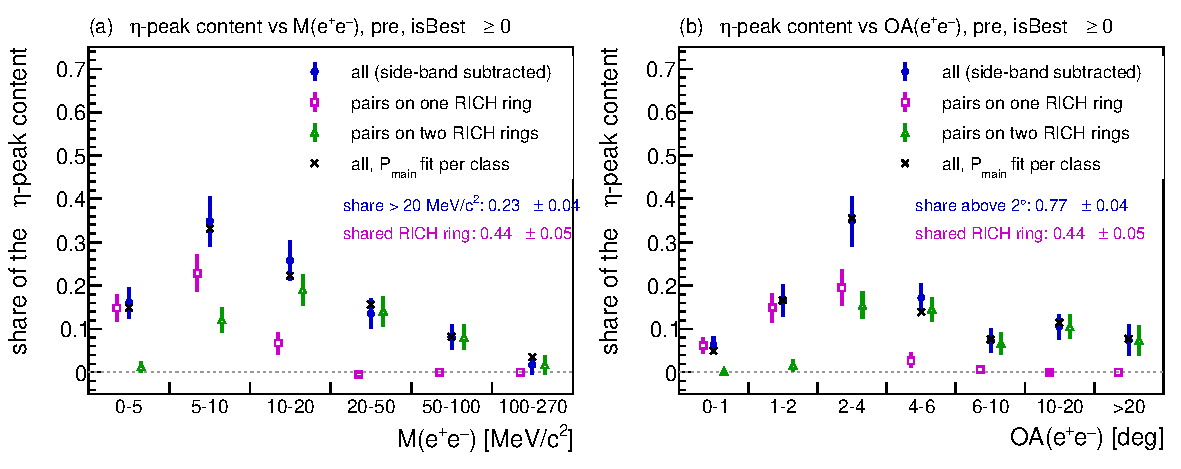
\includegraphics[width=\textwidth]{figs_exp/res_mee_content.pdf}
\caption{Content of the $\eta$ peak in classes of (a) \Mee [\MeVcc] and (b) OA [deg], as shares of the total; data, selection ``pre'', all
combinations (isBest $\ge0$). Selection: data with the base cuts \ptthreecap{}, an event vertex reconstructed ($\vz>-500$\,mm) and inside the target region ($\vz>-160$\,mm), particles identified by the START-free velocity \betanew (pions within $3\sigma$, leptons within $5\sigma$ of the expected band; leptons with a RICH ring), energy-loss-corrected momenta for all four tracks, all stored \ppee combinations of each event (isBest $\ge0$), no further cut (together ``pre''); classes (a) \Mee 0--5, 5--10, 10--20, 20--50, 50--100 and 100--270\,\MeVcc, (b) OA 0--1, 1--2, 2--4, 4--6, 6--10, 10--20 and above $20^\circ$; peak window $R_{\mathrm{pk}}$ 0.53364--0.55416\,\GeVcc, side bands $R_{\mathrm{SB}}$ 0.5225--0.53364 and 0.55416--0.56530\,\GeVcc; the CB of each class from its own like-sign counts. Blue: side-band subtraction in \Mfour, $S_{\mathrm{SB}}=[(N-\mathrm{CB})_{R_{\mathrm{pk}}}-r_{SB}(N-\mathrm{CB})_{R_{\mathrm{SB}}}]/(f_{\mathrm{pk}}-r_{SB}f_{SB})$,
$R_{\mathrm{pk}}$ $=$ 0.53364--0.55416, $R_{\mathrm{SB}}$ $=$ 0.5225--0.53364 and 0.55416--0.56530\,\GeVcc, $r_{SB}$ from the \Pmain pol2; stat $\oplus$ model. Magenta / green: pairs whose leptons
share one RICH ring / have two rings. Crosses: \Pmain fit of each class alone. CB of each class from its like-sign counts, $k=1$. Not
normalised to luminosity.}
\label{fig:res_mee}
\end{figure}

\subsection{A look at the X17 band}
\label{sec:x17}
Table~\ref{tab:res_x17} and Fig.~\ref{fig:res_x17} show the \Mee distribution of the $\eta$-peak counts for ``pre'' + both pions in the
vertex fit (the frozen X17 selection with the data peak window as X17 \Mfour window instead of the simulation window), with the
side-band method ($r_{SB}=0.9148$). In the X17 band $15.5\le\Mee<24.5$\,\MeVcc there are $N=5258$ counts, CB $=101.7$ ($N_{++}=14$, $N_{--}=223$), and
$D=481\pm99$ $\eta$-peak counts (isBest $=1$: $385\pm90$; OA$>2^\circ$: $487\pm99$, the window lies above $2^\circ$). A log-linear interpolation
from the two neighbouring \Mee bands expects $522\pm111$; the difference, $-40\pm149$, shows nothing. This is a look, not a test: a limit
needs the simulated X17 efficiency and resolution (\S\ref{sec:needsim}). The \Pmain content of the band ($440\pm92\pm60$, whole Gaussian)
agrees with $S_{\mathrm{SB}}=D/(f_{\mathrm{pk}}-r_{SB}f_{SB})=541\pm111$. Table~\ref{tab:x17win} gives the band in all three X17 \Mfour windows,
and Fig.~\ref{fig:opt_x17} draws them.

% res_x17_cnt.tex: copy of res_x17.tex with "rows" -> "counts" (analyst, 15 Nov 2026; Part II writer, integ4)
% res_x17.tex -- written by plots/exp_report/res_mee.C (numbers: tables_exp/res_mee.txt)
\begin{table}[H]
\centering\small
\setlength{\tabcolsep}{4pt}
\caption{The X17 band, data only: counts in the data $\eta$ peak window (0.53364--0.55416~GeV/$c^2$) for the selection pre + both pions in the vertex fit (frozen X17 selection with the data peak window as X17 $M_4$ window), in $M(e^+e^-)$ bands of 9~MeV/$c^2$ (bold: the X17 band). CB $=2\sqrt{N_{++}N_{--}}$ ($k=1$); background $=r\,(N-\mathrm{CB})_{R_\mathrm{SB}}$ from the $M_4$ side bands (0.5225--0.53364, 0.55416--0.56530) with $r=0.915$; $D$ = $\eta$-peak counts inside $R_\mathrm{pk}$ after the subtraction. All stored combinations (isBest $\geq0$); in brackets isBest $=1$. No limit is derived here: it needs the simulated X17 efficiency.}
\label{tab:res_x17}
\begin{tabular}{lrrrrr}
\toprule
$M_{ee}$ [MeV/$c^2$] & $N_\mathrm{pk}$ & CB$_\mathrm{pk}$ & $(N-\mathrm{CB})_\mathrm{pk}$ & background & $D$ \\
\midrule
6.5--15.5 & 23756 (19857) & 168.5 & $23587\pm157$ & $22047\pm145$ & $1540\pm211$ ($1434\pm192$) \\
\textbf{15.5--24.5} & 5258 (4369) & 101.7 & $5156\pm74$ & $4675\pm67$ & $481\pm99$ ($385\pm90$) \\
24.5--33.5 & 2657 (2227) & 99.1 & $2558\pm53$ & $2381\pm49$ & $177\pm71$ ($143\pm65$) \\
33.5--42.5 & 1876 (1565) & 123.6 & $1752\pm45$ & $1574\pm41$ & $178\pm60$ ($171\pm54$) \\
42.5--51.5 & 1436 (1167) & 173.3 & $1263\pm41$ & $1166\pm37$ & $96\pm53$ ($55\pm49$) \\
51.5--60.5 & 1149 (956) & 212.6 & $936\pm37$ & $895\pm34$ & $41\pm49$ ($74\pm44$) \\
\bottomrule
\end{tabular}
\end{table}


\begin{figure}[H]
\centering
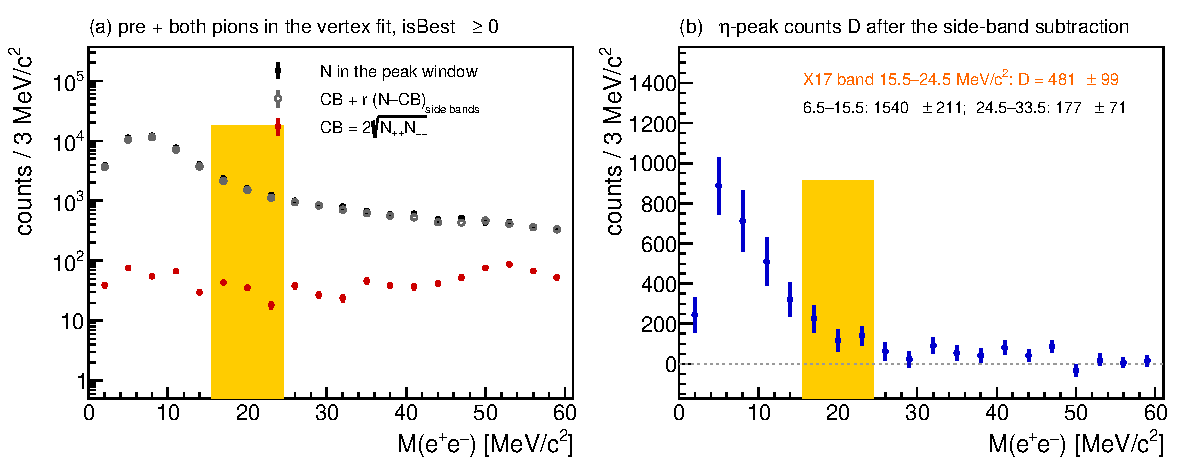
\includegraphics[width=\textwidth]{figs_exp/res_x17_window_cnt.pdf}
\caption{The X17 band, data only. Selection: data with the base cuts \ptthreecap{}, an event vertex reconstructed ($\vz>-500$\,mm) and inside the target region ($\vz>-160$\,mm), particles identified by the START-free velocity \betanew (pions within $3\sigma$, leptons within $5\sigma$ of the expected band; leptons with a RICH ring), energy-loss-corrected momenta for all four tracks, all stored \ppee combinations of each event (isBest $\ge0$) (together ``pre'') and both pion tracks used in the fit of the event vertex; counts in the data peak window $0.53364\le\Mfour<0.55416$\,\GeVcc (background under the peak from the side bands 0.5225--0.53364 and 0.55416--0.56530\,\GeVcc), all \Mee in 3\,\MeVcc bins; the X17 band $15.5\le\Mee<24.5$\,\MeVcc is only marked. Selection ``pre'' + both pions in the vertex fit, all combinations (isBest $\ge0$), counts in the data
$\eta$ peak window 0.53364--0.55416\,\GeVcc; 3\,\MeVcc bins of \Mee. (a) Black: $N$; red: CB ($k=1$); grey open: CB + $r_{SB}(N-\mathrm{CB})$ of the
\Mfour side bands (the background under the peak). (b) $D$ $=$ $\eta$-peak counts after the side-band subtraction. Orange band: the frozen X17
band 15.5--24.5\,\MeVcc. No limit is derived (it needs the simulated X17 efficiency). Counts, not normalised to luminosity.}
\label{fig:res_x17}
\end{figure}

\begin{figure}[tbp]% float since 15 Nov 2026 (an [H] here left a half-empty page)
\centering
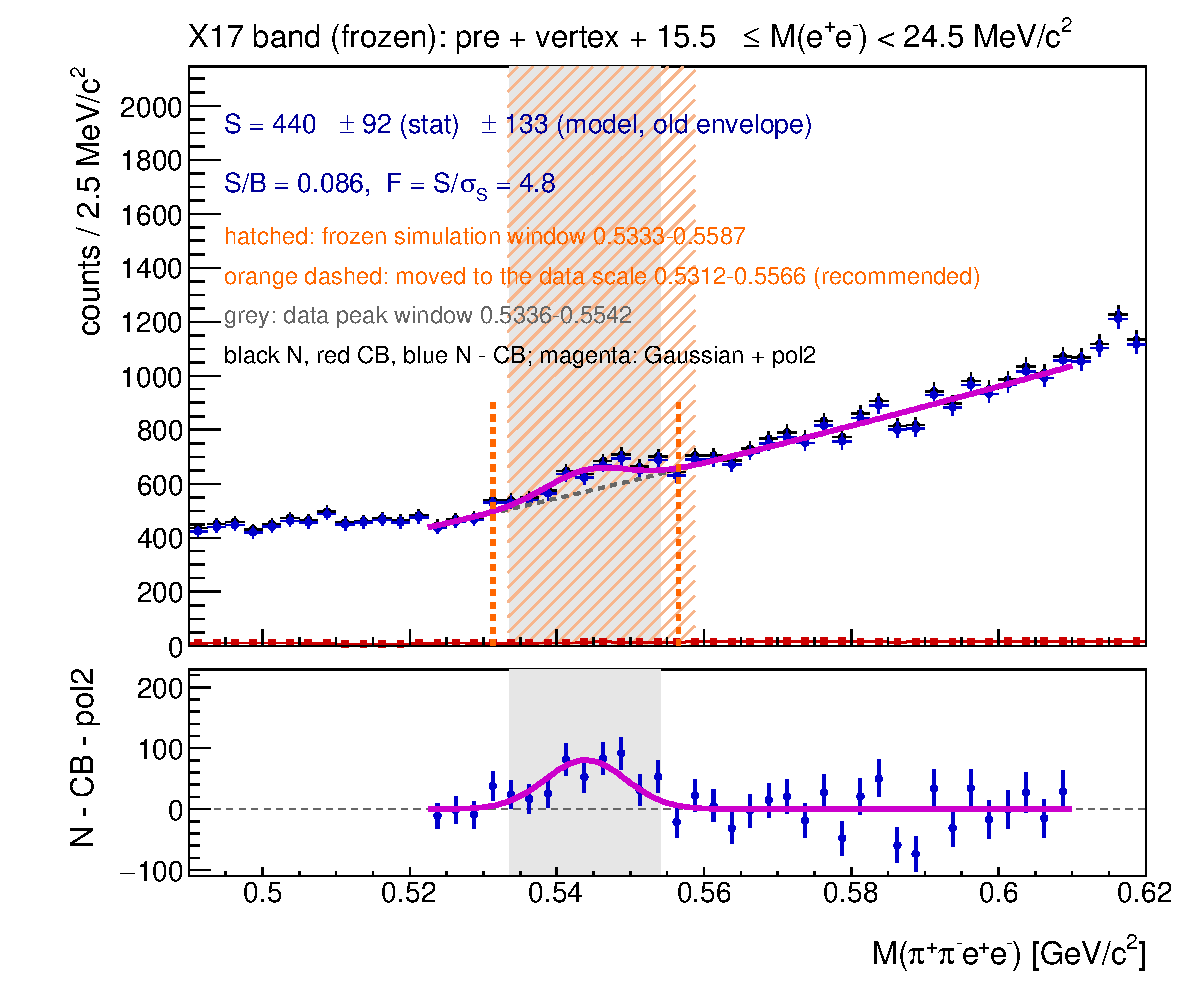
\includegraphics[width=0.9\textwidth]{figs_exp/opt_named_x17_cnt.pdf}
\caption{\Mfour in the frozen X17 band: ``pre'' + both pions in the vertex fit + $15.5\le\Mee<24.5$\,\MeVcc, all combinations (isBest $\ge0$). Selection: data with the base cuts \ptthreecap{}, an event vertex reconstructed ($\vz>-500$\,mm) and inside the target region ($\vz>-160$\,mm), particles identified by the START-free velocity \betanew (pions within $3\sigma$, leptons within $5\sigma$ of the expected band; leptons with a RICH ring), energy-loss-corrected momenta for all four tracks, all stored \ppee combinations of each event (isBest $\ge0$) (together ``pre''), both pion tracks used in the fit of the event vertex and $15.5\le\Mee<24.5$\,\MeVcc (the X17 band); the fit in 0.5225--0.6100\,\GeVcc uses no \Mfour window; the three X17 \Mfour windows are only marked.
The three X17 \Mfour windows of Table~\ref{tab:x17win}: hatched, frozen simulation window 0.5333--0.5587\,\GeVcc; orange dashed lines,
the recommended window moved to the data scale, 0.5312--0.5566; grey, data peak window. Same fit as in Fig.~\ref{fig:opt_named_spectra};
the Gaussian is the $\eta$ content of the \Mee band ($440\pm92\pm133$ counts with the old envelope; revised model uncertainty $\pm60$).
CB share 2\,\% ($k=1$). Counts, not normalised to luminosity.}
\label{fig:opt_x17}
\end{figure}

\textbf{Two later remarks.} (1) The CB of the band rests on few like-sign counts ($N_{++}=14$): the rule of this
report gives 101.7 counts, the geometric mean of the whole window 112 and the ``spread rule'' of Part~III $171\pm6$ (\S\ref{sec:cbmethod});
$D$ should hardly depend on it, because the CB enters the peak window and the side bands alike (not evaluated). (2) This side-band
subtracted \Mee spectrum was public before Part~III froze its X17 procedure, so the X17 search of Part~III is ``blind in the code, not in the
information'' (its decision D19). With the simulation, Part~III sets the limit
$\mathrm{BR}(\eta\to\pipi X17)\,\mathrm{BR}(X17\to\ee)<3.16\times10^{-5}$ (90\,\% CL$_s$, 17\,\MeVcc; X17 at most 11\,\% of the direct decays,
$r<0.114$, with the PDG 2026 BR$(\eta\to\ppee)$, D25).\footnote{The procedure frozen before the search used the PDG 2020 value of
BR$(\eta\to\ppee)$; with it the limit reads $3.06\times10^{-5}$.}

\subsection{Stability}
\label{sec:stab}
\textbf{Per period} (Table~\ref{tab:smp_peak_periods}, Figs.~\ref{fig:smp_periods}--\ref{fig:smp_spectra_nomvtx}): the $\eta$-peak yield per
luminosity is constant within the statistics, $\chi^2/\mathrm{ndf}=1.4/3$ ($p=0.70$, ``pre'', weighted mean $0.777\pm0.061$) and 1.6/3 ($p=0.65$,
peak nominal + vertex, $0.659\pm0.046$); days 034--044 against 045--067 give $1.00\pm0.16$ and $0.996\pm0.142$. The variants are also constant
(``pre'' + OA$>2^\circ$ 0.51/3, peak nominal + vertex + OA$>2^\circ$ 0.08/3, isBest $=1$ 1.38/3 and 0.91/3). The CB scale ($\pm3$\,\%) changes $S$ by less than
0.4\,\% in every period. With 11--30\,\% statistical errors per period these tests cannot see the 5\,\% effects of \S\ref{sec:rates}. $N-\mathrm{CB}$ in the
bump window per \nbinv (``pre'') follows the count rates: I $23.01\pm0.11$, IIA $24.92\pm0.31$, IIB $24.22\pm0.18$, III $21.90\pm0.13$ (III lower by
5\,\%; rms over the periods 4.9\,\%). A physical yield per luminosity should be constant. These steps follow the steps of the count rates
(\S\ref{sec:rates}); they are not an event-vertex effect on the $\eta$, whose vertex efficiency is consistent with 1 in every period within
1.7$\sigma$ ($\varepsilon_T=1.01$, 0.99, 0.92, 1.01 in I, IIA, IIB, III, code of the first vertex study; \S\ref{sec:vtxeff}). $W$ contains
21.7\,\% wall counts (``pre'', raw, \S\ref{sec:walls}); if the wall counts follow the halo level, $W$ per luminosity should change by III/I $=0.950$
and II/I $=1.072$, against 0.952, 1.083 (IIA) and 1.053 (IIB) observed: the steps of $W$ are consistent with $\eta$-free wall and halo counts
(an indication). Until their cause is confirmed, the integrated visible yields carry a period-normalisation uncertainty
of $\pm5$\,\% (Table~\ref{tab:syst}). Part~III tests the bump edge per period as well (uses the simulation): the edge step of the data
over the simulated step scaled to the luminosity of the period is 0.408, 0.342, 0.481 and 0.325 in I, IIA, IIB and III, compatible
with a constant ($\chi^2/\mathrm{ndf}=6.8/3$, $p=0.08$).

\textbf{Tagged $\eta$ per period} (Table~\ref{tab:res_period}, Fig.~\ref{fig:res_tagged_period}): $Y_T$ is low in period I (0.512 against 0.584--0.622
in IIB and III, 12--18\,\% lower; 7\,\% below the mean; $\chi^2/\mathrm{ndf}=6.3/3$, $p=0.10$). The sector-2 deficit cannot explain this: its measured
loss of counts is 3.0\,\% on days 034--044 (\S\ref{sec:rates}), and period I also contains days 045--046. The drop is consistent with a statistical
fluctuation ($p=0.10$). The peak yield does not show it (period I $0.83\pm0.09$, IIA $0.85\pm0.26$; for peak nominal + vertex IIB 0.701 lies above
I 0.698). $S/T$ falls from 1.62 (I) to 1.15 (III), $\chi^2/\mathrm{ndf}=3.1/3$.

\textbf{Halves of the data} (folds, Table~\ref{tab:folds}, numbers of \code{opt_named.txt}): the peak contents of the two folds agree within
1.8$\sigma$ (pulls $-1.79$ to $+0.49$; the largest for pre + vertex). The bump $E$ differs between the folds by $-1.4$ to $-3.0\sigma$ in every
selection except the X17 band (``pre'' $515\pm50$ against $683\pm50$, $-2.35\sigma$; first study without $\vz$ cut $-160\pm76$, $-2.1\sigma$).
With the bootstrap errors of $E$ (\S\ref{sec:fixmodel}; ratio 0.978 for ``pre'') ``pre'' gives about $-2.4\sigma$ (the first draft quoted
$-1.2$ to $-2.5\sigma$, ``pre'' $-2.0\sigma$, with the factor 1.2, which is not confirmed). All selections
share the same fold split and overlap strongly, so their pulls are correlated and have the same sign; over the 40 random halvings the mean
pull of $E$ is $-0.22\pm0.19$. Part~III finds the same split marginal for the edge scale on ``pre'' + vertex ($z=1.9$--2.0, $p\approx0.05$).
The fold asymmetry is consistent with a fluctuation of this one split.

\begin{table}[H]
\centering
\caption{$\eta$-peak content $S$ (\Pmain) and bump edge-step sum $E$ in the two halves of the event groups (fold $=$ parity of the group
index), data, all combinations (isBest $\ge0$); pull $=$ (fold 0 $-$ fold 1)/error with the fit errors as quoted (a bootstrap confirms the
fit errors of $E$ within 0.98--1.07, \S\ref{sec:fixmodel}; the division by 1.2 of the first draft is withdrawn). Numbers of
\code{tables_exp/opt_named.txt}. Counts, not normalised to luminosity.}
\label{tab:folds}
\small
\begin{tabular}{@{}l r r r r r r@{}}
\toprule
Selection & $S$ fold 0 & $S$ fold 1 & pull $S$ & $E$ fold 0 & $E$ fold 1 & pull $E$ \\
\midrule
``pre'' & $2140\pm259$ & $2528\pm259$ & $-1.06$ & $515\pm50$ & $683\pm50$ & $-2.35$ \\
pre + vertex & $1919\pm217$ & $2468\pm217$ & $-1.79$ & $513\pm42$ & $629\pm42$ & $-1.96$ \\
peak nominal & $2066\pm231$ & $2261\pm231$ & $-0.60$ & $484\pm48$ & $684\pm48$ & $-2.96$ \\
peak nominal + vertex & $1833\pm195$ & $2114\pm195$ & $-1.02$ & $477\pm40$ & $613\pm40$ & $-2.40$ \\
DIRECT & $1981\pm231$ & $2510\pm231$ & $-1.62$ & $530\pm45$ & $654\pm45$ & $-1.97$ \\
PEAK & $1986\pm219$ & $2378\pm219$ & $-1.26$ & $518\pm42$ & $602\pm42$ & $-1.43$ \\
bump nominal & $1354\pm167$ & $1278\pm168$ & $+0.32$ & $463\pm42$ & $618\pm42$ & $-2.59$ \\
bump nominal + vertex & $1251\pm142$ & $1153\pm142$ & $+0.49$ & $446\pm36$ & $558\pm36$ & $-2.20$ \\
X17 band & $185\pm65$ & $254\pm65$ & $-0.74$ & $56\pm13$ & $55\pm13$ & $+0.11$ \\
pre without $\vz>-160$\,mm & $2201\pm276$ & $2454\pm276$ & $-0.65$ & $541\pm54$ & $701\pm54$ & $-2.10$ \\
\bottomrule
\end{tabular}
\end{table}

% smp_peak_periods_cnt.tex: copy of smp_peak_periods.tex with "rows" -> "counts" (analyst, 15 Nov 2026; Part II writer, integ4)
% smp_peak_periods.tex -- written by plots/exp_report/smp_flow.C (numbers: tables_exp/smp_peak_periods.txt)
\begin{table}[H]
\centering\small
\setlength{\tabcolsep}{3pt}
\caption{$\eta$-peak content per period. $P_\mathrm{main}$: $\chi^2$ fit of $N-\mathrm{CB}$ (CB $=2\sqrt{N_{++}N_{--}}$, $k=1$) with the frozen Gaussian (0.5439~GeV/$c^2$, $\sigma=5.4$~MeV) and a second-order polynomial in 0.5225--0.6100~GeV/$c^2$; $S$ = whole Gaussian $\pm$ stat $\pm$ model spread (old envelope). All stored combinations (isBest $\geq 0$), corrected momenta, PT3, $v_z>-160$~mm. $s=Y_S=S\times\frac{64}{63}/L$ in visible counts per nb$^{-1}$, $L$ = START-free luminosity of the analysed runs; visible yield, not corrected for acceptance or efficiency. Constancy over I, IIA, IIB, III with the statistical errors.}
\label{tab:smp_peak_periods}
\begin{tabular}{lr rr rr}
\toprule
 & & \multicolumn{2}{c}{pre} & \multicolumn{2}{c}{peak nominal + vertex} \\
Period (days) & $L$ [nb$^{-1}$] & $S$ & $s$ [counts/nb$^{-1}$] & $S$ & $s$ [counts/nb$^{-1}$] \\
\midrule
I (034-046) & 2809.5 & $2287\pm251\pm577$ & $0.827\pm0.091$ & $1931\pm189\pm431$ & $0.698\pm0.068$ \\
IIA (047-048) & 372.6 & $310\pm94\pm74$ & $0.845\pm0.257$ & $180\pm69\pm84$ & $0.490\pm0.188$ \\
IIB (049-053) & 1078.0 & $870\pm159\pm252$ & $0.820\pm0.150$ & $744\pm118\pm194$ & $0.701\pm0.111$ \\
III (059-067) & 1819.1 & $1203\pm193\pm343$ & $0.672\pm0.108$ & $1093\pm148\pm313$ & $0.611\pm0.082$ \\
\midrule
034-044 (sector-2 deficit) & 2449.2 & $1883\pm233\pm518$ & $0.781\pm0.097$ & $1586\pm176\pm328$ & $0.658\pm0.073$ \\
045-067 & 3630.0 & $2788\pm283\pm724$ & $0.780\pm0.079$ & $2361\pm213\pm607$ & $0.661\pm0.060$ \\
\midrule
all 29 days & 6079.2 & $4671\pm367\pm958$ & $0.780\pm0.061$ & $3949\pm276\pm936$ & $0.660\pm0.046$ \\
\midrule
$\chi^2/\mathrm{ndf}$ (I, IIA, IIB, III) &  & \multicolumn{2}{c}{1.4/3 ($p=0.70$)} & \multicolumn{2}{c}{1.6/3 ($p=0.65$)} \\
\bottomrule
\end{tabular}
\end{table}


\begin{figure}[H]
\centering
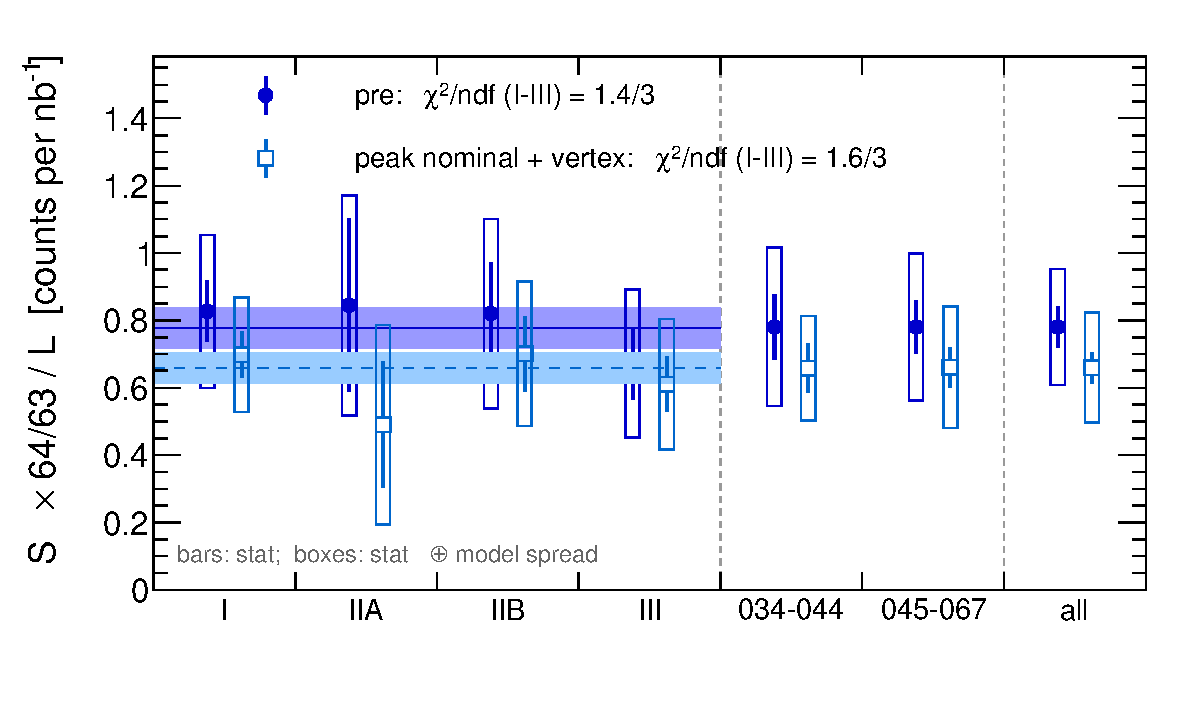
\includegraphics[width=0.9\textwidth]{figs_exp/smp_peak_periods_cnt.pdf}
\caption{$\eta$-peak content per \nbinv, $s=Y_S=S\times\frac{64}{63}/L$ in visible counts per \nbinv, per period, for days 034--044 against 045--067, and for all days. Selection: data with the base cuts \ptthreecap{}, an event vertex reconstructed ($\vz>-500$\,mm) and inside the target region ($\vz>-160$\,mm), particles identified by the START-free velocity \betanew (pions within $3\sigma$, leptons within $5\sigma$ of the expected band; leptons with a RICH ring), energy-loss-corrected momenta for all four tracks, all stored \ppee combinations of each event (isBest $\ge0$) (together ``pre'', full circles) and ``pre'' with angle between the \pipi and the \ee momenta in the laboratory $\alab<55^\circ$, $\Mpipi>0.30$\,\GeVcc and both pion tracks used in the fit of the event vertex (peak nominal + vertex, open squares); periods by beam-time day: I 034--046, IIA 047--048, IIB 049--053, III 059--067 (days 054--058 absent), and the day groups 034--044 and 045--067; fit range 0.5225--0.6100\,\GeVcc. ``pre'' (full
circles) and peak nominal + vertex (open squares), all combinations (isBest $\ge0$). $S$ from \Pmain (CB $=2\sqrt{N_{++}N_{--}}$, $k=1$, frozen Gaussian
0.5439\,\GeVcc / 5.4\,\MeVcc + pol2 in 0.5225--0.6100). Bars: statistical error; boxes: stat $\oplus$ model spread. Bands: weighted mean over I--III (stat).
$L$ = START-free luminosity of the analysed runs; visible yield, not corrected for acceptance or efficiency.}
\label{fig:smp_periods}
\end{figure}

\begin{figure}[!htb]
\centering
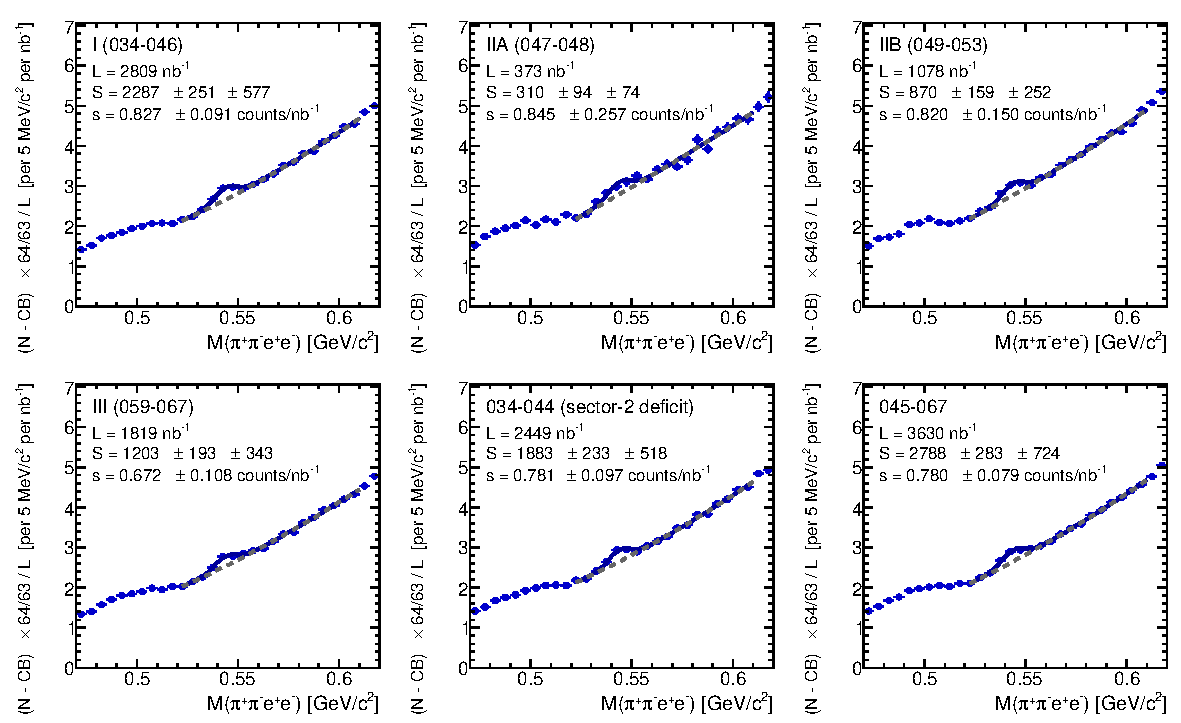
\includegraphics[width=0.95\textwidth]{figs_exp/smp_peak_spectra_pre_cnt.pdf}
\caption{$N-\mathrm{CB}$ per \nbinv ($\times64/63$) in 5\,\MeVcc bins around $m_\eta$ for the periods I, IIA, IIB, III and for days 034--044 and 045--067;
selection ``pre'', all combinations (isBest $\ge0$), CB with $k=1$. Selection: data with the base cuts \ptthreecap{}, an event vertex reconstructed ($\vz>-500$\,mm) and inside the target region ($\vz>-160$\,mm), particles identified by the START-free velocity \betanew (pions within $3\sigma$, leptons within $5\sigma$ of the expected band; leptons with a RICH ring), energy-loss-corrected momenta for all four tracks, all stored \ppee combinations of each event (isBest $\ge0$), no further cut (together ``pre''); periods by beam-time day: I 034--046, IIA 047--048, IIB 049--053, III 059--067 (days 054--058 absent), and the day groups 034--044 and 045--067. Solid: \Pmain fit (fitted in 2.5\,\MeVcc bins); dashed: its polynomial.
$S\pm$stat$\pm$model (old envelope), $s=Y_S=S\times\frac{64}{63}/L$ (visible counts per \nbinv). Equal y ranges. Visible yields, not corrected for acceptance or efficiency.}
\label{fig:smp_spectra_pre}
\end{figure}

\begin{figure}[!htb]
\centering
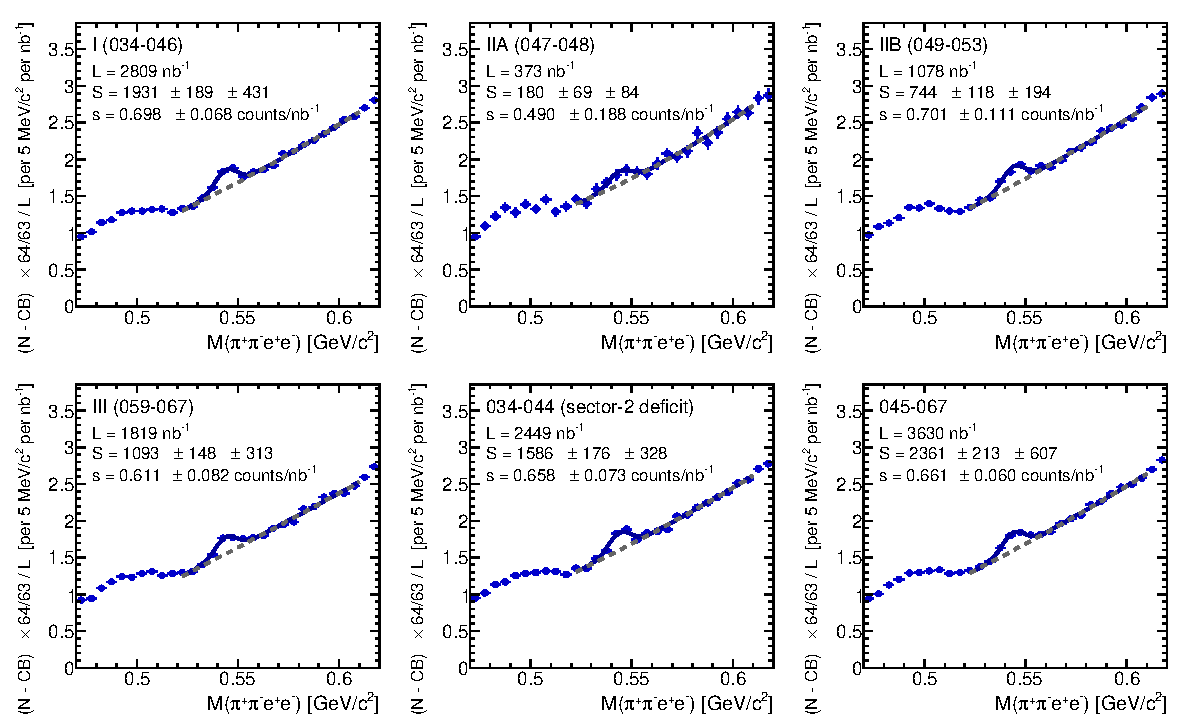
\includegraphics[width=0.95\textwidth]{figs_exp/smp_peak_spectra_nomvtx_cnt.pdf}
\caption{As Fig.~\ref{fig:smp_spectra_pre} for the selection peak nominal + vertex ($\alab<55^\circ$, $\Mpipi>0.30$\,\GeVcc, both pions in the vertex fit),
isBest $\ge0$. Selection: data with the base cuts \ptthreecap{}, an event vertex reconstructed ($\vz>-500$\,mm) and inside the target region ($\vz>-160$\,mm), particles identified by the START-free velocity \betanew (pions within $3\sigma$, leptons within $5\sigma$ of the expected band; leptons with a RICH ring), energy-loss-corrected momenta for all four tracks, all stored \ppee combinations of each event (isBest $\ge0$) (together ``pre''), angle between the \pipi and the \ee momenta in the laboratory $\alab<55^\circ$, $\Mpipi>0.30$\,\GeVcc and both pion tracks used in the fit of the event vertex; periods by beam-time day: I 034--046, IIA 047--048, IIB 049--053, III 059--067 (days 054--058 absent), and the day groups 034--044 and 045--067.}
\label{fig:smp_spectra_nomvtx}
\end{figure}

% wr_res_period_cnt.tex: copy of wr_res_period.tex with "rows" -> "counts" (analyst, 15 Nov 2026; Part II writer, integ4)
% wr_res_period.tex -- copy of res_period.tex (identical since the review fix of 2026-11-14); original written by plots/exp_report/res_peak.C (numbers: tables_exp/res_peak.txt)
\begin{table}[H]
\centering\small
\setlength{\tabcolsep}{4pt}
\caption{ECAL-tagged $\eta$ content $T$ (counts with a photon, $0.119\leq M(e^+e^-\gamma)<0.173$~GeV/$c^2$, $m_{ee}<0.10$; frozen $m_{5c}$ peak 0.5463~GeV/$c^2$, 6.2~MeV/$c^2$, pol2) and the ratio of the $\eta$-peak content $S$ ($P_\mathrm{main}$) to $T$ per period of the beam time, selection pre, isBest $\geq0$; $Y_T=T\times\frac{64}{63}/L_\mathrm{period}$ in visible counts per nb$^{-1}$; statistical errors only (the model spread is common). $S$ per period is identical to Table~\ref{tab:smp_peak_periods}, where the peak yield per period is given. Last rows: weighted mean and $\chi^2$/ndf of a constant. Sector 2 had a trigger deficit on days 034--044 (period I) that is not in $L$; its measured loss of counts, 3\,\%, is too small to explain the low $Y_T$ of period I.}
\label{tab:res_period}
\begin{tabular}{lrrccc}
\toprule
Period & $L$ [nb$^{-1}$] & $S$ & $T$ & $Y_T$ [counts/nb$^{-1}$] & $S/T$ \\
\midrule
I & 2809.5 & $2287\pm251$ & $1415\pm70$ & $0.5115\pm0.0253$ & $1.62\pm0.19$ \\
IIA & 372.6 & $310\pm94$ & $193\pm27$ & $0.5267\pm0.0730$ & $1.60\pm0.54$ \\
IIB & 1078.0 & $870\pm159$ & $660\pm46$ & $0.6220\pm0.0438$ & $1.32\pm0.26$ \\
III & 1819.1 & $1203\pm193$ & $1046\pm57$ & $0.5844\pm0.0317$ & $1.15\pm0.19$ \\
\midrule
all & 6079.2 & $4671\pm367$ & $3314\pm105$ & $0.5537\pm0.0175$ & $1.41\pm0.12$ \\
weighted mean & & & & $0.5522\pm0.0175$ & $1.38\pm0.12$ \\
$\chi^2$/ndf ($p$) & & & & 6.3/3 (0.10) & 3.1/3 (0.37) \\
\bottomrule
\end{tabular}
\end{table}


\begin{figure}[!htb]
\centering
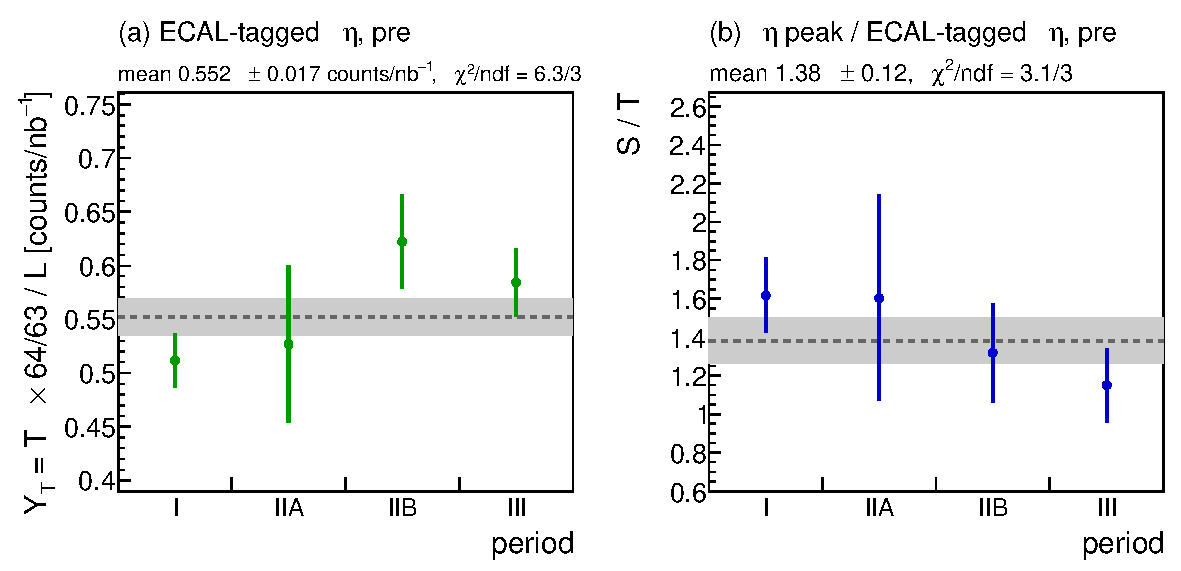
\includegraphics[width=0.9\textwidth]{figs_exp/res_tagged_period_cnt.pdf}
\caption{ECAL-tagged $\eta$ per period (I: 034--046, IIA: 047--048, IIB: 049--053, III: 059--067), selection ``pre'', all combinations
(isBest $\ge0$). Selection: data with the base cuts \ptthreecap{}, an event vertex reconstructed ($\vz>-500$\,mm) and inside the target region ($\vz>-160$\,mm), particles identified by the START-free velocity \betanew (pions within $3\sigma$, leptons within $5\sigma$ of the expected band; leptons with a RICH ring), energy-loss-corrected momenta for all four tracks, all stored \ppee combinations of each event (isBest $\ge0$) (together ``pre''); for $T$ an ECAL photon identified as a photon with $0.8<\beta<1.2$ and energy above 100\,MeV (of up to three such photons the one with $M(\ee\gamma)$ closest to 0.140\,\GeVcc), $0.119\le M(\ee\gamma)<0.173$\,\GeVcc and $\Mee<0.10$\,\GeVcc, fit in $0.49\le m_{5c}<0.62$\,\GeVcc; for $S$ in (b) the same ``pre'' counts without the photon condition, fit in $0.5225\le\Mfour<0.6100$\,\GeVcc. (a) $Y_T=T\times\frac{64}{63}/L_{\mathrm{period}}$ in visible counts per \nbinv with the START-free luminosity of the period; (b) ratio of the $\eta$-peak
content $S$ (\Pmain) to $T$. Statistical errors only; grey band: weighted mean $\pm$ error. Sector 2 had a trigger deficit on days 034--044 that is
not in $L$. Visible yields, not corrected for acceptance or efficiency.}
\label{fig:res_tagged_period}
\end{figure}

\subsection{The \texorpdfstring{$\eta$}{eta} efficiency of the mandatory event-vertex cut}
\label{sec:vtxeff}
\textbf{Why it was open.} FAT keeps only entries with an event vertex, $\vz>-500$\,mm (mandatory). PAT copies the vertex of the DST, where
\code{HParticleVertexFind} (\code{setCut(-170,-30,20)}) fits a vertex only if at least two tracks point into $-170<z<-30$\,mm within 20\,mm of
the beam axis; otherwise $\vz=-1000$\,mm. The cut removes 32.3\,\% of the \ee counts (0.565 survive in the peak window, \S\ref{sec:cutflow}), and the
$\eta$ content of the removed counts was not known. It was measured after the review (three studies of the PAT files; the decisive one by an
independent verifier with own code; notes \code{docs/latex/notes_all/ve_verify_note.md}, \code{ve_data_note.md}, \code{ve_sim_cause_note.md};
the full account is in Part~III, section ``$\eta$ efficiency of the event-vertex requirement'' there).

\textbf{Procedure} (data only, with the measures of this report):
\begin{enumerate}\setlength{\itemsep}{0pt}
\item Every entry of the 29 PAT day files with isBest $\ge0$, PT3 and \code{cor_ok}, \emph{without} any vertex requirement, is read directly
      (\code{plots/all_report/vtx_fill.C}). The entries with a vertex are exactly the FAT entries (4\,783\,467 / 122\,875 / 371\,524).
\item The entries are split into whole events with a vertex (V, $\vz>-500$\,mm) and without (Nv, $\vz=-1000$\,mm). Each class gets its own CB
      $=2\sqrt{N_{++}N_{--}}$ from its own like-sign counts ($k=1$). The cut $\vz>-160$\,mm is not applied (Nv has no \vz); Table~\ref{tab:vzslices}
      already shows that the counts with a vertex below $-160$\,mm hold no $\eta$.
\item The $\eta$ is measured in each class with the three frozen measures of this report: $S$ (\Pmain), $T$ (ECAL tag), $E$ (edge step).
      Because the CB of Nv has a statistical hole at $m_\eta$ (below), $S$ is also taken with a \emph{smooth like-sign CB}: $N_{++}$ and $N_{--}$
      of the class are each fitted with a polynomial (pol3, pol4 or pol5, from 0.45 or 0.48 to 0.66 or 0.70\,\GeVcc: 12 variants;
      $\chi^2=94.9/95$ and 100.5/95 for pol4 in 0.45--0.70), the CB is $2\sqrt{f_{++}f_{--}}$ per 2.5\,\MeVcc bin, and \Pmain is fitted as before;
      the quoted $S$ is the mean of the 12 variants (rms 30 counts). This is not the CB convention of this report (decision (ix)).
\item The efficiency is $\varepsilon_{\mathrm{vtx}}=X_V/(X_V+X_{Nv})$ for each measure $X$; the classes are disjoint events, so the errors of
      $X_V$ and $X_{Nv}$ are independent; $E$ carries its fit error $\times1.2$, a conservative choice kept from the first draft (the
      bootstrap of \S\ref{sec:fixmodel} finds the fit error right; with the plain fit error the combined result is 0.9934 instead of 0.9937). The three values $S$ (smooth CB), $T$ and
      $E$ are combined with inverse-variance weights as if independent; they use the same Nv events ($S$ and $T$ share about 30\,\% of the counts),
      but $T$ carries 81\,\% of the weight.
\end{enumerate}

\begin{table}[H]
\centering
\caption{$\eta$ efficiency of the mandatory cut $\vz>-500$\,mm, data, 29 PAT day files, PT3, all combinations (isBest $\ge0$), \code{cor_ok}; V:
counts with an event vertex, Nv: without. Errors: nominal-CB $S$ with the event-group factor and the model rms (verifier's grid: order 1--4, upper
bound 0.58--0.65, lower bound 0.5225--0.5275, width $\pm0.5$\,\MeVcc; 152 pairs with $p>0.05$); the other $S$ counts plain fit errors (the group
factor, 1.02--1.03, changes $\varepsilon$ by less than 0.002); $E$: fit error $\times1.2$ (conservative) $\pm$ model (18 variations applied to both classes).
The nominal-CB $S$ is shown but not used (see text). V contains ``pre'' and adds the counts with $-500<\vz\le-160$\,mm ($S=-19\pm133$): $S(\mathrm{V})
=4657$ against $S(\mathrm{pre})=4671$, $T(\mathrm{V})=3297$ (verifier's code) against 3314 (this report); the differences are within the errors. Last line: the simulation (Part~I samples, same
selection), for comparison only. Counts, not normalised to luminosity. Sources: \code{tables_all/vtx_ana.txt}, \code{vtx_ana2.txt},
\code{vtx_ana3.txt}, \code{vtx_sim.txt}, \code{vtx_numbers.txt}, \code{fix2_numbers.txt}.}
\label{tab:vtxeff}
\footnotesize
\begin{tabularx}{\textwidth}{@{}>{\raggedright\arraybackslash}p{5.4cm} r r L@{}}
\toprule
measure & $X_V$ & $X_{Nv}$ & $\varepsilon_{\mathrm{vtx}}$ \\
\midrule
$S$, nominal CB & $4657\pm397$ & $902\pm411$ & $0.838\pm0.063\pm0.060$ \\
$S$, unlike-sign counts only (no CB) & $4646\pm370$ & $165\pm324$ & $0.966\pm0.065$ \\
$S$, smooth like-sign CB & $4670\pm370$ & $263\pm324$ & $0.947\pm0.063$ \\
$T$, ECAL-tagged $\eta$ & $3297\pm110$ & $-4\pm77$ & $1.001\pm0.023$ \\
$E$, bump edge step & $1241\pm91$ & $21\pm96$ & $0.983\pm0.075\pm0.028$ \\
\midrule
\textbf{$S$ (smooth CB) $+$ $T$ $+$ $E$} & & & $\mathbf{0.994\pm0.021}$ ($\chi^2=0.7/2$; $>0.96$ at 95\,\% CL) \\
$S$ (nominal CB) $+$ $T$ $+$ $E$ & & & $0.990\pm0.022$ ($\chi^2=3.3/2$; CB convention of this report) \\
survival of the \ee counts (not an efficiency) & & & 0.565 (peak window), 0.677 (all) \\
simulation, $\eta$ classes C4+C5 & & & $0.99970\pm0.00002$ \\
\bottomrule
\end{tabularx}
\end{table}

\begin{figure}[tp]
\centering
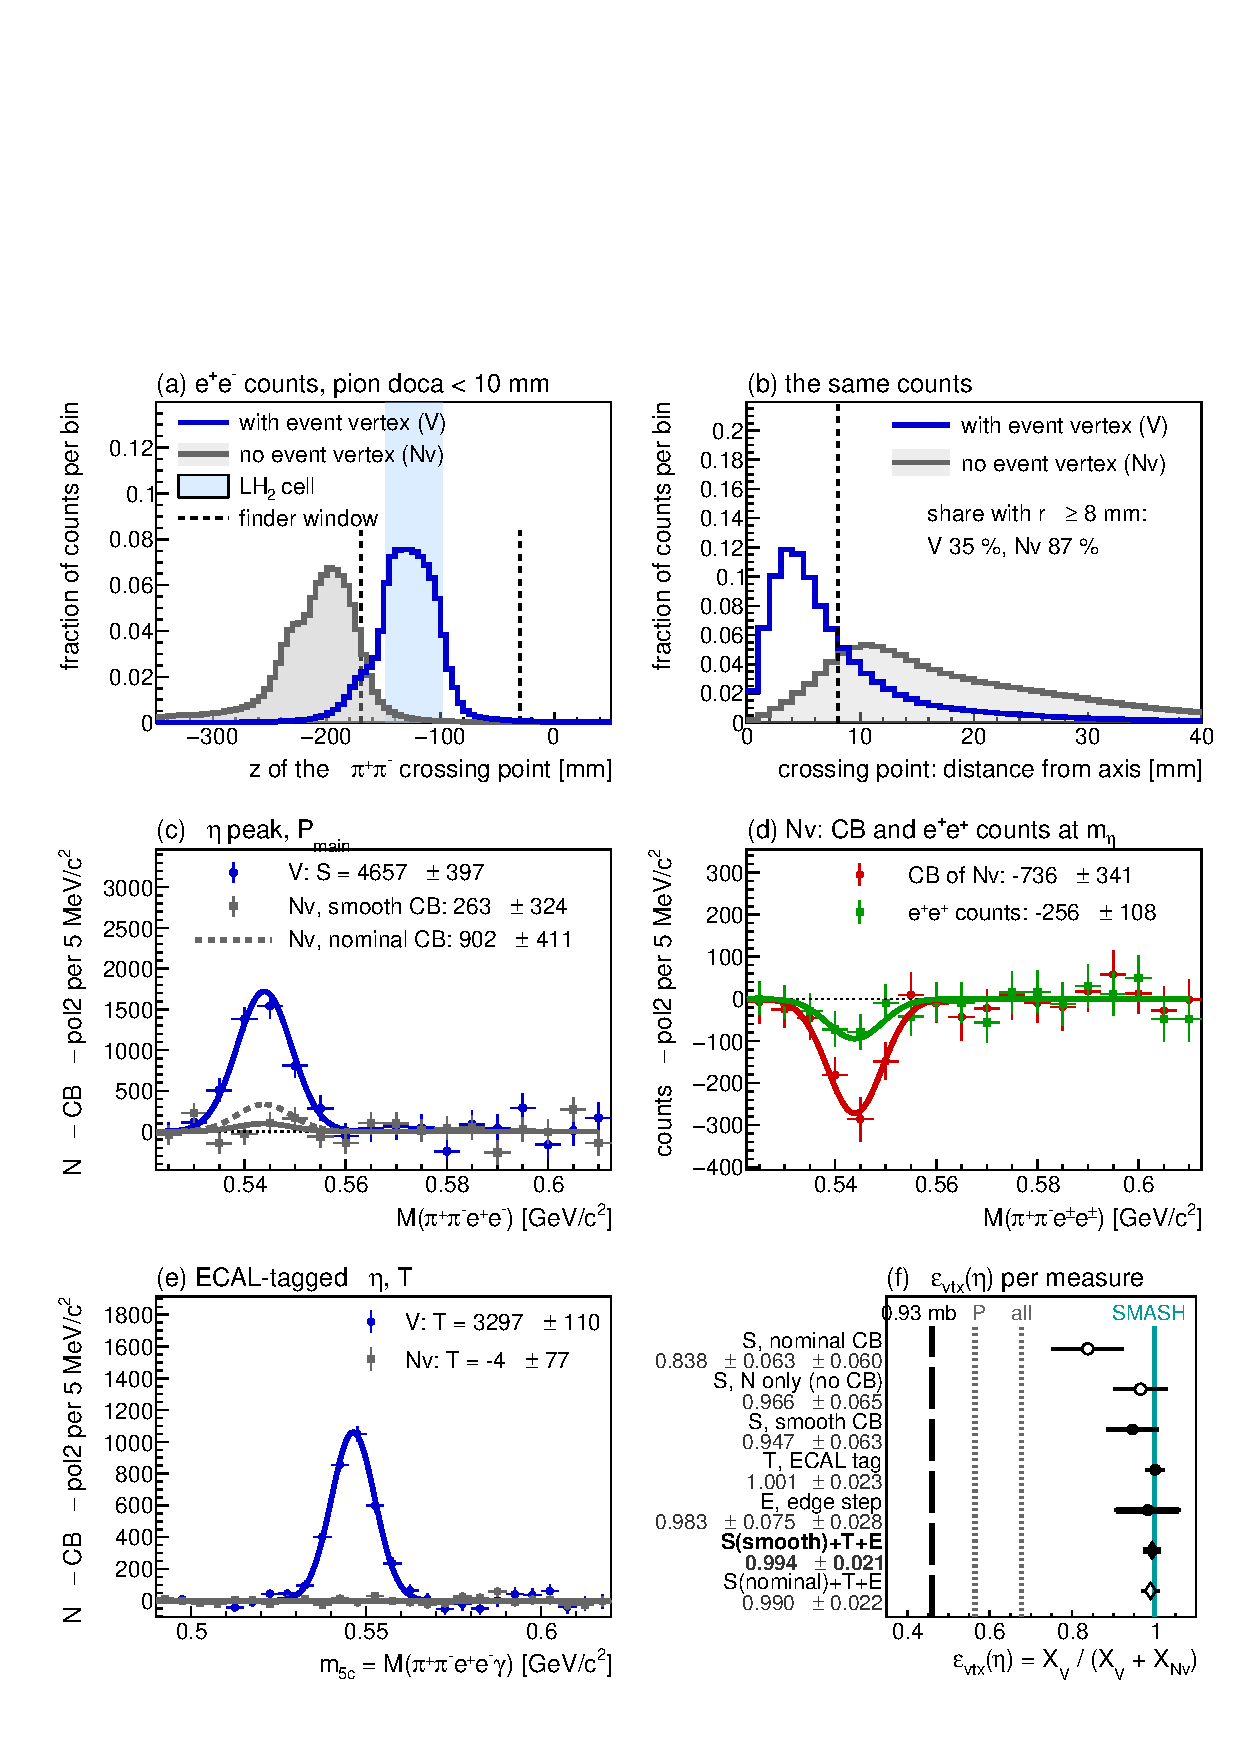
\includegraphics[width=0.95\textwidth]{figs_exp/fix2_vtx_fig_cnt.pdf}
\caption{$\eta$ efficiency of the mandatory cut $\vz>-500$\,mm. Selection: data, every entry of the 29 PAT day files with the \ptthreecap{}, \betanew identification (pions $3\sigma$, leptons $5\sigma$, leptons with a RICH ring), corrected momenta of all four tracks and isBest $\ge0$, without a vertex requirement, split into whole events with (V, $\vz>-500$\,mm) and without an event vertex (Nv, $\vz=-1000$\,mm); no target-region cut; (e) photon tag as in Fig.~\ref{fig:res_tagged}. Data, 29 PAT day files, PT3, isBest $\ge0$, \code{cor_ok}; counts with an event vertex
(V) blue, without (Nv) grey; counts, not normalised to luminosity. (a, b) $z$ and distance from the beam axis of the crossing point of the two pion
tracks (\ee counts, pion distance of closest approach $<10$\,mm; unit area); the Nv $z$ is partly shaped by the selection (at most one track in the
finder window). (c) $\eta$ peak, $N-\mathrm{CB}-$pol2 of the \Pmain fit (5\,\MeVcc bins): V; Nv with a smooth like-sign CB (squares: pol4,
0.48--0.70; legend: mean of the 12 variants) and, dashed, with the nominal CB; nominal-CB errors with the event-group factor. (d) Nv only: the
frozen Gaussian fitted to the CB (red) and to the $e^+e^+$ counts (green, the like-sign key of this report). (e) ECAL-tagged $\eta$ in m5c. (f)
$\varepsilon_{\mathrm{vtx}}$ as in Table~\ref{tab:vtxeff} (open: not used for the result; $E$: thick bar stat $\times1.2$, conservative, thin bar with the model
rms); lines: simulation 0.9997, survival of the counts 0.565 and 0.677, and 0.46, which 0.93\,mb would need in Part~III. Macro
\code{plots/all_report/fix2_vtx_fig.C}.}
\label{fig:vtxeff}
\end{figure}

\textbf{Results.} The tagged $\eta$ ($T$) and the bump edge ($E$, no ECAL) are zero in Nv, and the peak content with a smooth like-sign CB is
consistent with zero there: combined, the cut keeps $\varepsilon_{\mathrm{vtx}}(\eta)=0.994\pm0.021$ of the $\eta$ ($0.990\pm0.022$ if $S$ is
taken with the nominal CB). The nominal-CB $S$ (0.838) is not an $\eta$ loss: the unlike-sign counts of Nv alone show no peak ($165\pm324$), but
the CB of Nv has a dip of $-736\pm341$ counts at $m_\eta$, made by the $e^+e^+$ counts ($-256\pm108$, a 2.4$\sigma$ downward fluctuation); the
like-sign counts lose their vertex 2.2--2.4 times more often than the \ee counts, so the CB is 58\,\% of $N$ in Nv, and this hole turns into a fake
$S$(Nv) of 902 counts. (The fake peak is also $3.75\pm1.0$\,\MeVcc wide, 1.65$\sigma$ below the detector resolution: weak support only, since a
2$\sigma$ peak can fluctuate that much.) The ECAL tag works without an event vertex (the \piz peak in $M(\ee\gamma)$ is present in Nv,
5.5\,\MeVcc lower and 36\,\% wider, because the photon direction then uses the cluster vertex). Per period, with the code of the first vertex
study (ve\_data; its overall value $0.992\pm0.020$), $\varepsilon_T=1.013\pm0.033$, $0.993\pm0.097$, $0.924\pm0.045$, $1.006\pm0.030$ (I, IIA,
IIB, III): consistent with 1 in every period within 1.7$\sigma$ (IIB is the lowest). The nominal-CB $S$ of period III gives $0.700\pm0.088$
($S(\mathrm{Nv})=515\pm196$); about half of it is a dip of the CB (verifier), and $T$ and $E$ show nothing there.

\textbf{Where the counts without a vertex come from.} The evidence that does not depend on the selection: 87\,\% of their pion pairs cross
8\,mm or more from the beam axis (35\,\% of the counts with a vertex; Fig.~\ref{fig:vtxeff}b), which the finder does not cut on; their pp-elastic
content is $0.028\pm0.003$ of that of the cell (hadron production, three days; the elastic acceptance of upstream events was not modelled); their
CB$/N$ in the peak window is 0.58 (0.13 with a vertex); their share of the \ee counts follows the beam periods (days 034--045: 0.31, 046--053:
0.37, 059--067: 0.275), not the detector; and when the two pions cross inside the cell, only 0.15\,\% of the counts lack a vertex. These events
are therefore mostly not p+p on hydrogen in the cell. Their pion pairs cross at $z\approx-200$\,mm, 5--6\,cm in front of the upstream end of the
LH$_2$ cell ($-148$ to $-99$\,mm; 7--8\,cm from its centre); this position is partly forced by the selection (a count without a vertex has at most
one track in the finder window). There the target holder, the beam tube and its flanges sit (HGeant geometry). Beam halo on this material is a
likely source, but a hypothesis: it does not explain why these counts hold no $\eta$ at all, although p+A collisions at 4.5\,GeV make $\eta$
mesons. The cut is therefore validated: it removes non-target background, not target $\eta$.

\textbf{Later evidence for the halo hypothesis} (data only; Part~III). (1) The empty-target runs show directly that halo events on the material
in front of the cell exist at a large rate: counts at $-200\le\vz<-170$\,mm, off the beam axis, with the same composition and the same \vz
shape in empty and full runs (\S\ref{sec:walls}); in the full data these counts show no $\eta$ peak ($-19\pm76$, Table~\ref{tab:vzslices}), a
weak test (not sensitive, by the verifier vw2b). (2) Their rate follows the halo level, as does the share of the counts
without a vertex (0.31, 0.37, 0.275 in the three groups of days). (3) That share is flat over the sectors (0.317--0.327) and higher in events
without a START hit (0.53 against 0.30), as for particles that miss the START detector; the counts with \code{evtStart} $=0$ are 17\,\% of the counts
without a vertex and 7\,\% of those with one, and they hold no $\eta$ either ($-11\pm164$ counts). (4) The median track $z$ of the counts without a
vertex stays at $-214$ to $-197$\,mm at all polar angles, which the selection does not force (a timing or reconstruction distortion would change
with the angle). (5) The apparent loss of the nominal-CB $S$ sits only where the pions cross 8\,mm or more from the axis ($1.001\pm0.037$ at
$r<5$\,mm), where the CB of these counts has its hole; frozen-width fits at 39 other positions in these counts give pulls of rms 0.93, so their
errors are right. The open question remains why neither these counts nor the wall counts carry measurable $\eta$ (\S\ref{sec:openq}). An
check without the ECAL tag (Part~III): $S$ (smooth CB) and $E$ alone give $\varepsilon_{\mathrm{vtx}}=0.961\pm0.049$. (The K$^0_S$ does lose its vertex more often: the
cut keeps 0.72--0.85 of it. Its pions are displaced, and its part without a vertex does not sit in the upstream box of the pion crossing, 2.2
per $10^4$ counts there against 18.1 elsewhere (ve\_data), which supports the displaced decay as the reason.)

\textbf{Consequence for this report.} The visible yields are not corrected for it: a correction would raise them by $0.6\pm2.1$\,\% (at most
$+4$\,\% at 95\,\% CL; Table~\ref{tab:syst}). For the comparison with the simulation the cut needs no special treatment beyond this: the
simulation keeps 0.9997 of its $\eta$ counts, and Part~III quotes the ratio $1.006\pm0.021$ as a one-sided $+2$\,\% systematic. The simulation
still provides the efficiencies of all the other cuts (\S\ref{sec:needsim}).

\subsection{Summary of the uncertainties of the data side}
\label{sec:syst}
Table~\ref{tab:syst} collects the uncertainties of the data side for the recommended peak selection (PEAK) and the bump measure ($E$ of
``pre''). It is a list for the next step, not a final error budget: the efficiency-related items need the simulation.

\begin{table}[!t]% float (not [H]) since 15 Nov 2026: the longer table must not leave a nearly empty page before the appendices
\centering
\caption{Uncertainties of the data side, recommended selections (PEAK for the peak, ``pre'' for the bump; all combinations isBest $\ge0$).
Values relative to $S$ or $E$ unless stated; ``not corr.'': known effect not corrected in the visible yield; for one-sided items the sign
says in which direction the visible yield $Y$ would move if the effect were corrected. Notation: Table~\ref{tab:notation}.}
\label{tab:syst}
\footnotesize
\begin{tabularx}{\textwidth}{@{}>{\raggedright\arraybackslash}p{5.0cm} >{\raggedright\arraybackslash}p{3.6cm} L@{}}
\toprule
Source & Size & Remark \\
\midrule
statistics (fit) & PEAK 7.1\,\%; $E$ 5.9\,\% & per-count Poisson fit errors; right for $S$ (halves) and $E$ (bootstrap); earlier $\times1.2$ for $E$ not confirmed (\S\ref{sec:fixmodel}) \\
model, $S$ (edge-safe grid rms) & PEAK 477 counts (10.9\,\%) & 144 variations, lower bounds $\ge0.5225$; old envelope 867 (19.9\,\%) \\
model, $E$ (18 variations per slice) & 287 counts (24\,\%) & half ranges added over the slices \\
peak position & free fit PEAK $S=4287\pm450$ & position not varied in the model spread; $\pm0.6$\,\MeVcc between selections \\
CB scale $\pm3$\,\% & $\le0.07$\,\% ($S$), $\le0.1$\,\% ($E$) & absorbed by the pol2; $W$ moves by 0.1--0.5\,\% \\
CB $\times k_{\mathrm{mix}}$ & PEAK $+0.28$\,\%; $E$ $+0.7$\,\% & $k_{\mathrm{mix}}$ 1.01--1.04, pool spread 0.01 \\
CB normalisation (plain sum bound) & PEAK $-0.1$\,\% ($\le1$\,\%); $E$ $+2.3$\,\% & CB $+38$--45\,\%; $W$ up to $-7$\,\%: CB$/N$, $W$ have an unknown scale \\
CB binning / interpolation & $-0.6$\dots$+1.3$\,\% (PEAK) & statistical noise of the CB; not to be added \\
CB: $e^-e^-$ step in $u$ & 39 counts of the $u$ step (3\,\%) & pairs from the two \piz photons, subtracted with their \ee partners (CB right, verified); $S$ unaffected (\S\ref{sec:cbnull}, D39, approved) \\
tail of the $\eta$ peak, $u$ fit & $h_u$ 1217--1308 & size not fixed by the data; Part~III: $t=1\pm0.5$ (D40, approved) (\S\ref{sec:edgeu}) \\
sculpting $S_{\mathrm{fake}}$ & $+48\pm27$ or $+83\pm26$ counts (1.1--1.9\,\%) & one-sided; two implementations (\S\ref{sec:sculpt}) \\
bump fold asymmetry & $-2.35\sigma$ (``pre''; $-2.4\sigma$ with bootstrap errors) & consistent with a fluctuation of the fold split \\
\midrule
luminosity \Lsf & $\pm6.9$\,\% & 5.56\,\% HADES, 1.03\,\% fit, 4.0\,\% normalisation; stat 5.2\,\nbinv \\
vertex condition of elastic $L$ & not checked & none: upstream elastic events add about 1\,\% to $L$; DST vertex: several \% possible (\S\ref{sec:lumi}) \\
PT3 live fraction & one-sided, $Y$ up to $+7.3$\,\% & $L\times0.932$ if it applies; data cannot decide \\
sector-2 trigger deficit & one-sided, $Y$ $+1.2$\,\% (1.4\,\% with day 045) & counts lost on days 034--044 (045); not in $L$, not corr.; day 045: lepton channel only (elastic PT2/PT3 1.074, $L$ right) \\
START-based sorter loss & one-sided, $Y$ $+1.3$--1.6\,\% or $+2.2$--2.8\,\% & $L$ is corrected for it, the yields are not; not measurable in the output (decision viii) \\
combined one-sided & $Y$ up to about $+11$\,\% & sum of the three items above (7.3 + 1.2 + 2.8\,\%) \\
target walls (empty target) & one-sided, $Y$ lower by $3^{+4}_{-3}$\,\% if subtracted (12\,\% at the nucleon-count expectation) & measured (\S\ref{sec:walls}); not subtracted; window counts hold 16--24\,\% wall counts (``pre'', raw) \\
period normalisation & $\pm5$\,\% on the integrated $Y$ & rates change in steps (rms 4.9\,\%), \S\ref{sec:stab}; not a vertex effect on the $\eta$; steps follow the halo (indication) \\
event-vertex cut $\vz>-500$\,mm & $\varepsilon_{\mathrm{vtx}}(\eta)=0.994\pm0.021$: $Y$ $+0.6\pm2.1$\,\% ($\le+4$\,\%, 95\,\% CL) & measured (\S\ref{sec:vtxeff}); the 32\,\% of counts it removes (0.565 survive in P) are mostly non-target background; not corr. \\
\code{trigbit} $=12288$, \code{no_hf} runs & 0.007\,\%; $+0.2$ counts & negligible \\
\midrule
\code{cor_ok} rule (entries dropped) & fallback $+2.4$\,\% of $S$ & acceptance effect: the simulation must apply the same rule \\
\bottomrule
\end{tabularx}
\end{table}

%======================================================================
\section{What needs the simulation}
\label{sec:needsim}
%======================================================================

\inshort{The efficiencies, the bump yield, the branching ratio, the split into direct decay and conversion, the X17 limit and the transfer of the mass scale need the simulation of Part~I. Part~III has since done most of them; its results are quoted below as cross-references (data + simulation).}
The data alone give visible yields, shapes and checks; the following steps need the simulation of Part~I and are the subject of the next
report.
\begin{enumerate}\setlength{\itemsep}{0pt}
\item \textbf{Efficiencies.} Acceptance $\times$ efficiency of the recommended selections, with the same rules as here: all combinations
      (isBest $\ge0$), the PID polygons (the data pion bands are 30--50\,\% wider than the simulated ones), the \code{cor_ok} rule
      (\S\ref{sec:corok}), the vertex flag (data $\varepsilon_S=0.940\pm0.041$ on the base ``peak nominal''; Part~III, on its base S0/``pre'': data
$0.941\pm0.052$ against simulation 0.940, ratio $1.002\pm0.056$), \dzpi (data and
      simulation agree to 4\,\%), \MMfour (simulation generated at 4500\,MeV, analysed at 4530), the PT3 trigger. The event-vertex cut
      $\vz>-500$\,mm is no longer on this list: its $\eta$ efficiency is measured in the data ($0.994\pm0.021$, \S\ref{sec:vtxeff}; the
      simulation keeps 0.9997 of its $\eta$ counts), and the counts it removes are mostly non-target background that the simulation does not contain. Data-side corrections that the simulation does not contain must be added: the sector-2 deficit, the
      START-sorter loss, the live fraction, the target walls (Part~III applies $1-f_\eta=0.97$, D21, approved by the analyst on 15 November 2026;
      \S\ref{sec:walls}), and the period normalisation ($\pm5$\,\%). \emph{Part~III} turns the peak into
      $\sigma(pp\to\eta X)=0.43\pm0.17\,(\mathrm{measurement})\,^{+0.08}_{-0.03}\,(\mathrm{model})$\,mb (the measurement error includes the
      peak-tail term of D40, approved), labelled PRELIMINARY: by the analyst's
      ruling of 15 November 2026 the label stays because the make-up of the peak is open ($\pm32$\,\%; D28), and the production-model item
      (the extrapolation with the $\eta$ kinematics of SMASH) is quoted apart (D29).
\item \textbf{The bump yield.} $E$ is not a yield. The extraction needs the simulated bump shape; in the blind test of Part~I the side band with
      the simulated shape had a bias of $+3.9$\,\%, the edge step $+1.3$\,\% with a 16\,\% error, the template fit $+7.7$\,\%.
      \emph{Done in Part~III} (data + simulation): the bump is measured in the distance to the edge, $u$ (\S\ref{sec:edgeu}),
      $0.426\pm0.020\pm0.034\pm0.030$ of SMASH and $21\,468\pm1003\pm1708\pm1347$ counts in the bump window (``pre'' + vertex); this is the
      bump measurement of Part~III (D37, approved; $\sigma(pp\to\eta X)$ from the bump 0.444\,mb, PRELIMINARY as the peak). The per-slice
      edge is its cross-check: $0.423\pm0.023\pm0.038\pm0.048$ of SMASH (0.392 without the C2 correction), a visible bump yield of
      $21\,445\pm1152\pm1900\pm2223$ counts. Both scales weight every simulated C2 Dalitz decay with its QED decay-angle weight (D38, approved:
      the simulation decays the virtual photon isotropically; the per-count weights raise the scales by 1.4\,\% ($u$) and 1.2\,\% (per slice)
      over the earlier constant factor, and they are applied until a future simulation corrects the angle in GEANT itself, which is not
      expected); the
      side band with the simulated shape (B4) is \emph{not determined} in the data (157\,\% systematic; a quadratic background term moves it by
      $+150$\,\%, the $u$ edge by $-2.2$\,\%). The $u$ fit also needs the shape of the low-mass tail of the $\eta$ peak, which reaches the
      edge (\S\ref{sec:edgeu}). The data cannot fix its size ($t=0.3\pm1.0$ times the simulated tail), so Part~III takes half of the
      simulated tail as a systematic term: $\pm3.4$\,\% on $f_\eta(u\text{-edge})$, $\pm3.6$\,\% on the per-slice edge, $\pm8.8$\,\% on
      $\sigma(pp\to\eta X)$ from the peak side bands (D40, approved by the analyst on 15 November 2026, option (a)). A larger simulated sample of $\eta\to\pipi\gamma$ (now 180 simulated entries in
      the fit region), a simulation with the radiation of the decay itself, and the peak position against \Mpipi in the data would settle it.
\item \textbf{The branching ratio.} In the ratio of the peak to the bump the luminosity and much of the acceptance cancel. Both
      contain conversion components: the peak $\eta\to\pipi\gamma$ with a converted photon (about 40\,\% by \S\ref{sec:mee}), the bump
      $\eta\to\pipi\piz$, $\piz\to\gamma\gamma$ with one converted photon. The conversion probability (the material) does not cancel in the
      ratio, so both components must be subtracted with the simulated material before the ratio gives $\mathrm{BR}(\eta\to\ppee)$ relative to
      $\mathrm{BR}(\eta\to\pipi\piz)\,\mathrm{BR}(\piz\to\ee\gamma)$; the tagged $\eta$ is a second reference once the ECAL efficiency and
      calibration are known. \emph{Part~III} (ECAL study): the full reconstruction with the ECAL photon keeps about 12\,\% of the bump, as a
      clean peak; the data hold $1.16\pm0.21$ of the prediction with the simulated photon energy scale and $0.84\pm0.15$ with a data-like one
      (errors overestimated); before it can be a measurement it needs the photon energy scale and resolution in data and simulation, the module
      efficiency (65\,\% in the simulation, not explained), a photon cut that does not depend on START (or a simulated START efficiency) and at
      least 10 times more simulated $\eta\to\pipi\piz$. \emph{Part~III}: the double ratio peak/bump from the edge is $0.97\pm0.10\pm0.17\pm0.12$
      (data over SMASH; without the peak-composition term; with it, as quoted for the $u$ edge, $0.97\pm0.37$); the
      branching ratio from the template fits of the pairs above 20\,\MeVcc relative to the bump, $2.67\times10^{-4}$, is a cross-check only
      (130\,\% total uncertainty).
\item \textbf{Direct decay and conversion.} The split of the peak needs the simulated acceptance per mode in \Mee and OA. Part~I found a tension
      in the OA$>2^\circ$ efficiency of the peak: simulation $0.697\pm0.015$ (with the physics weights) against $0.778\pm0.033$ in the data
      (Part~I's data number); this part gives $0.772\pm0.037$ (side band) and 0.778 (ratio of the \Pmain contents), \S\ref{sec:mee}.
      \emph{Part~III} (with the simulated shapes): conversion route $0.237\pm0.049$ and direct decays $0.497\pm0.059$ of SMASH; the data peak has
      more pairs above $\Mee=10$\,\MeVcc than SMASH (share $0.546\pm0.053$ against 0.425). The reading ``about 40\,\% conversions'' of
      \S\ref{sec:mee} therefore stays provisional; Part~III's decision D32 considers a loss of close pairs in the data. The analyst ruled on
      15 November 2026 that it is to be tested in a separate analysis: the reconstruction efficiency of \ee pairs with an opening angle of
      0--6$^\circ$ in data and simulation, from \piz, $\eta$ and $\omega$ Dalitz decays with the \ee hypothesis plus the ECAL photon, after the
      trigger-bias correction and the new ECAL calibration (both in progress).
\item \textbf{X17.} The efficiency of the frozen X17 cuts (Part~I's $s_1$, the expected X17 counts per unit branching ratio), the \Mee
      resolution and scale in data (not checked), the X17 \Mfour window on the data mass scale, and a background constrained from the data side bands instead of the simulated one (the expected limit of Part~I,
      $1.9\times10^{-5}$, is set by the simulation statistics of the background). \emph{Done in Part~III}: two-dimensional fit with the
      background from the \Mfour side bands in every \Mee bin, $r<0.114$ and $\mathrm{BR}<3.16\times10^{-5}$ (90\,\% CL$_s$, 17\,\MeVcc; expected
      $2.7\times10^{-5}$; PDG 2026, D25).\footnote{With the PDG 2020 value of BR$(\eta\to\ppee)$ of the frozen procedure:
      $3.06\times10^{-5}$.}
\item \textbf{Mass scale.} The transfer of the K$^0_S$ scale ratio (simulation/data $1.0048\pm0.0007$) to \Mfour is not verified.
      \emph{Part~III} does not transfer it: it uses the $\eta$ peak itself ($M_4'=0.99615\,M_4$ for the simulation); the \Mpipi transfer 0.9952 is
      confirmed by the K$^0_S$ position (data/simulation $0.9997\pm0.0011$).
\item \textbf{Rules.} No simulation-to-data spectrum comparison without per-channel cross-section scaling (the absolute data/simulation scale is
      known only to 15--20\,\%); the simulation has no CB, so it never gives $k$ or a CB number, and like-sign or CB rates of the data are never
      compared with simulated ones; simulated like-sign entries only help to identify the origin and kinematics of a structure seen in the data
      (for example the $e^-e^-$ step in $u$: pairs from the two \piz photons, \S\ref{sec:cbnull}).
\end{enumerate}

\howpart{Appendices: reference material}

\appendix

%======================================================================
\section{Notation and abbreviations}
\label{app:notation}
%======================================================================
The full notation of Part~II (moved here from the front of the report); the symbols needed for Section~\ref{sec:results} are
also listed in \S\ref{sec:symbols}. A count is one stored \pip\pim$e^+e^-$ combination (one ntuple entry); with isBest $\ge0$ an event can
give more than one count.

{\footnotesize
\setlength{\tabcolsep}{4pt}
\renewcommand{\arraystretch}{1.06}
\begin{longtable}{@{}>{\raggedright\arraybackslash}p{3.0cm} >{\raggedright\arraybackslash}p{\dimexpr\textwidth-3.0cm-2.2cm-4\tabcolsep\relax} >{\raggedright\arraybackslash}p{2.2cm}@{}}
\caption{\textbf{Notation and abbreviations} of Part~II. Last column: where the item is defined in
detail. Code names of the ntuple columns are given in typewriter font where they appear in tables.}
\label{tab:notation}\\
\toprule
Symbol & Meaning & Details \\
\midrule
\endfirsthead
\toprule
Symbol & Meaning & Details \\
\midrule
\endhead
\bottomrule
\endfoot
\multicolumn{3}{@{}p{\dimexpr\textwidth-2\tabcolsep\relax}}{\emph{Symbols that mean something else in Part~I:} $F$ (Part~I: $F_{\mathrm{I}}=S/\sqrt{S+B}$ on simulation), $T$ (here the tagged content; the beam energy is $T_{\mathrm{beam}}$), $W$, $Q$ (defined below).} \\
\multicolumn{3}{@{}l}{\textbf{Data, production and bookkeeping}} \\
DST, PAT, FAT & reconstructed data; PostDST Analysis Tool (hypotheses, PID, relative times, ranking); Final Analysis Tool (selection, kinematics, ntuples) & \S\ref{sec:prod}, \S\ref{sec:chain} \\
day file, \code{file_id} & one merged PAT output per day of the beam time (\code{lep_034} \dots\ \code{lep_067}); its day number & Tab.~\ref{tab:smp_samples} \\
period I, IIA, IIB, III & groups of days 034--046, 047--048, 049--053, 059--067 (luminosity periods) & Tab.~\ref{tab:smp_lumi} \\
count & one stored combination \pip\pim$\ell\ell$ of tracks of a hypothesis (one ntuple entry); with isBest $\ge0$ an event can give more than one count & \S\ref{sec:hyp} \\
event group & adjacent entries with equal (\code{file_id}, run, event); unit of the errors of window counts, fractions and side-band numbers (fit errors are per-count Poisson errors) & \S\ref{sec:groups} \\
$n_g$, var$/N$ & counts of one event group in a window; $\sum_g n_g^2$ over the counts: event-group factor of the variance & \S\ref{sec:groups} \\
$T_{\mathrm{beam}}$, $\sqrt{s}$ & beam kinetic energy, 4530\,MeV in all kinematics; c.m.\ energy, $\sqrt{s}=3.467$\,GeV & \S\ref{sec:beam} \\
isBest & PAT ranking of the combinations of an event: 1 best, 0 others; ``all combinations'' $=$ isBest $\ge0$ (main variant), isBest $=1$ comparison & \S\ref{sec:hyp} \\
us, pp, mm; $N$, $N_{++}$, $N_{--}$ & unlike-sign (\pipi\ee), like-sign (\pipi$e^+e^+$, \pipi$e^-e^-$) hypotheses; their counts & \S\ref{sec:hyp} \\
PT3, PT2, \code{trigbit} & PT3: the main reaction trigger, fullSecMult\,$\ge2$ and iTOFPadMult\,$\ge3$ (at least two sectors with an inner-TOF hit in coincidence with TOF or RPC, and at least three inner-TOF paddles hit); PT2: minimum bias, fullSecMult\,$\ge1$, downscaled by 64; \code{trigbit}: the trigger bit, only the first-arriving bit is written (PT3 events 8192; PT2 and PT2\,\&\,PT3 events 4096); this analysis keeps bit 8192 (P.~Tlusty, HADES internal presentation, 13 December 2024) & \S\ref{sec:fat} \\
\code{cor_ok} & all four energy-loss corrected momenta are finite & \S\ref{sec:corok} \\
\vz & z of the reconstructed event vertex (\code{eVertReco_z}), mm; $-1000$ when the DST vertex finder found fewer than two tracks in its window & \S\ref{sec:cutflow} \\
V, Nv; $\varepsilon_{\mathrm{vtx}}$ & counts with an event vertex ($\vz>-500$\,mm) / without ($\vz=-1000$\,mm); $\eta$ efficiency $X_V/(X_V+X_{Nv})$ of the cut $\vz>-500$\,mm for a measure $X$ ($S$, $T$, $E$) & \S\ref{sec:vtxeff} \\
smooth like-sign CB & vertex study only: $N_{++}$ and $N_{--}$ of a class each fitted with a polynomial $f_{\pm\pm}$ (pol3, pol4 or pol5, from 0.45 or 0.48 to 0.66 or 0.70\,\GeVcc: 12 variants); CB $=2\sqrt{f_{++}f_{--}}$ per 2.5\,\MeVcc bin; $S$ $=$ mean of the 12 variants (rms 30 counts) & \S\ref{sec:vtxeff} \\
``pre'' & base selection: \code{cor_ok}$=1$, isBest $\ge0$, $\vz>-160$\,mm (FAT: $\vz>-500$\,mm, PT3) & \S\ref{sec:sel} \\
\code{no_hf} run & run flagged in the luminosity table with $L=0$ (``drop its events'') & \S\ref{sec:lumi} \\
fold & parity of the event-group index; splits the data into two independent halves & \S\ref{sec:groups} \\
\midrule
\multicolumn{3}{@{}l}{\textbf{Luminosity and normalisation}} \\
\Lsf & START-free integrated luminosity (elastic scattering, six sectors) of all 17\,615 runs, 6080.5\,\nbinv & \S\ref{sec:lumi} \\
\Lan & the same summed over the 17\,557 runs present in the data, 6079.2\,\nbinv & \S\ref{sec:lumi} \\
$L_{\mathrm{LGAD}}$ & luminosity with the LGAD START condition (publication chain), 5587.5\,\nbinv & Tab.~\ref{tab:smp_lumi} \\
$f_{\mathrm{LF}}$ & PT3/PT2 live-fraction ratio LF3/LF2$\,\times\,64/63$ as defined in the luminosity files (0.932 overall; 0.9334 with our $L$ weighting) & \S\ref{sec:lumi} \\
$64/63$ & trigger-bit factor: bit 8192 holds 63/64 of the PT3 events & \S\ref{sec:lumi} \\
$Y_N$, $Y_S$, $Y_T$ & visible yield per luminosity, $X\times\frac{64}{63}/L$ in \emph{visible counts per \nbinv} (counts, not events; not a cross section; not corrected for acceptance or efficiency), of the counts $N$ (or $N-\mathrm{CB}$), of the peak content $S$ (written $Y$ in the result tables and $s$ in Table~\ref{tab:smp_peak_periods} and Figs.~\ref{fig:smp_periods}--\ref{fig:smp_spectra_nomvtx}), of the tagged content $T$ & Eq.~(\ref{eq:yield}) \\
$R$ & counts of ``pre'' per day $\times\,64/63/L$ (rate per day) & \S\ref{sec:rates} \\
$\sigma_{\mathrm{int}}$ & elastic cross section integrated over the acceptance, used for $L$ (2.90699\,mb) & \S\ref{sec:lumi} \\
target walls, empty target & Mylar windows of the LH$_2$ cell and the material around it; runs with the cell empty (days 034, 047, 065; 127 runs) & \S\ref{sec:walls} \\
$U$, $b$ & counts of the channel (\ee + like-sign) with $-200\le\vz<-170$\,mm (beam halo on material in front of the cell); flux ratio $U_{\mathrm{full}}/U_{\mathrm{empty}}$ of the same day & \S\ref{sec:walls} \\
$U/L$, $h$ & halo level: front counts per \nbinv; $h=100\,U/N$, front counts per 100 counts of ``pre'' + vertex & \S\ref{sec:walls} \\
\fwin & share of the target walls in the counts of a window, $b\,Y_{\mathrm{empty}}/Y_{\mathrm{full}}$ (luminosity-weighted over the three days); describes the background, never applied to $\eta$ yields & Tab.~\ref{tab:walls} \\
\feta, $r$ & share of the target walls in the $\eta$ signal, $3^{+4}_{-3}$\,\% (Part~III, D21, approved); $\eta$ per count in the walls over that in hydrogen ($0.07\pm0.30$) & \S\ref{sec:walls} \\
$\varepsilon_{s2}$, $C_{\mathrm{sec}}$ & double-ratio efficiency of the counts with a sector-2 track on the deficit days; Part~III's correction of the $\eta$ yields for it (span 034--045 approved, D26) & \S\ref{sec:rates} \\
PT2 check & elastic events in sector~2 over the mean of the other sectors, relative to the clean days 046--067, per day (analyst's table) & Tab.~\ref{tab:s2pt2} \\
$R_{\mathrm{sort}}$, $s_{\mathrm{lost}}$, $T_{\mathrm{DS}}$ & sorter correction of the luminosity analysis; share of the affected elastic events that is really lost (0.544); $1-$ share of down-scaling passengers (0.960--0.970) & \S\ref{sec:sorter} \\
\midrule
\multicolumn{3}{@{}l}{\textbf{Particle identification}} \\
$\betanew$ & velocity from the time differences of the tracks of a hypothesis (START-free) & Eq.~(\ref{eq:tnew}) \\
$\beta_{\mathrm{DST}}$ & DST velocity measured against the START time & \S\ref{sec:sorter} \\
reference track & the track whose time offset is shared with the others ($e^-$ in \ppee) & \S\ref{sec:pid} \\
$n\sigma$ polygon, v1, v6 & PID cut at $n$ standard deviations in ($p$, $\betanew$); data cut file \code{betanew_v1}, simulation \code{betanew_v6} & Tab.~\ref{tab:pid_polygons} \\
ring, \code{kIsLepton} & RICH ring correlated with the track (lepton slot); track-sorter lepton flag & \S\ref{sec:pid} \\
lepton / hadron pass & the two passes of the DST track sorter (DST $\beta\ge0.9$ / $\beta\ge0$ and tof $\le60$\,ns) & \S\ref{sec:sorter} \\
class A, B; $r_B$ & counts with both leptons $\beta_{\mathrm{DST}}\ge0.9$ / at least one below; share of the $\eta$ signal in class B ($r$ in Tab.~\ref{tab:pid_peak_dstbeta}) & Tab.~\ref{tab:pid_peak_dstbeta} \\
\midrule
\multicolumn{3}{@{}l}{\textbf{Kinematic variables and cuts}} \\
\Mfour ($M_4$), \Mee ($M_{ee}$, $m_{ee}$), \Mpipi ($M_{\pi\pi}$) & invariant masses of \ppee, of the \ee pair, of the \pipi pair (corrected momenta) & \\
mass scale & fitted position / nominal mass: of the $\eta$ peak in \Mfour, of K$^0_S$ in \Mpipi & \S\ref{sec:scale} \\
$\Delta z_{\pi\pi}$, DOCA & distance in $z$ of the crossing point of the two pion tracks from \vz; their distance of closest approach (K$^0_S$ selection) & Tab.~\ref{tab:res_scale} \\
\MMfour & missing mass of \ppee: mass of (beam + target $-$ \ppee), $T_{\mathrm{beam}}=4530$\,MeV & Tab.~\ref{tab:cuts} \\
$p_{T,4}$, $y_4$ & transverse momentum (lab) and c.m.\ rapidity of \ppee & Tab.~\ref{tab:cuts} \\
OA & opening angle of $e^+$ and $e^-$ (lab); OA$>2^\circ$ is a variant, never a fixed cut & Tab.~\ref{tab:cuts} \\
\alab (\code{oa_lab}) & angle between the \pipi and \ee momenta (lab) & Tab.~\ref{tab:cuts} \\
\aeta ($\eta$-rest angle) & angle between \pipi and \ee in the rest frame of a hypothetical $\eta$ (measured \ppee momentum, mass $m_\eta$) & Tab.~\ref{tab:cuts} \\
\dzpi & $\max(|z_{\pi^+}-\vz|,|z_{\pi^-}-\vz|)$, $z$ of a track at its closest approach to the beam axis & Eq.~(\ref{eq:dzpi}) \\
``vertex'' & both pions used in the event-vertex fit (\code{pip_isUsedVertex} and \code{pim_isUsedVertex}) & Tab.~\ref{tab:cuts} \\
peak / bump nominal & data-optimised kinematic selections of the first study & Tab.~\ref{tab:named} \\
slides, old code & earlier selections with the cut $\aeta>140^\circ$ & Tab.~\ref{tab:named} \\
PEAK, DIRECT, BUMP, X17 & selections frozen in the simulation study (Part~I) & Tab.~\ref{tab:frozen} \\
X17 band, X17 \Mfour window & ``pre'' + both pions in the vertex fit + $15.5\le\Mee<24.5$\,\MeVcc (called ``X17 region'' in some tables and figures); the \Mfour window applied to it (simulation, moved, or data window) & Tab.~\ref{tab:x17win} \\
peak / bump window (data) & $0.53364\le\Mfour<0.55416$ / $0.4550\le\Mfour<0.5225$\,\GeVcc & Tab.~\ref{tab:windows} \\
peak / bump window (sim.) & $0.5333$--$0.5587$ / $0.4576$--$0.5255$\,\GeVcc (simulation-centred) & Tab.~\ref{tab:windows} \\
side bands, $R_{\mathrm{pk}}$, $R_{\mathrm{SB}}$ & 0.5225--0.53364 and 0.55416--0.56530\,\GeVcc; peak-window and side-band regions of the side-band method & \S\ref{sec:proc} \\
bump, peak & $\eta\to\pipi\piz$ seen below $m_\eta$ (photon lost); $\eta$ at $m_\eta$ ($\eta\to\ppee$ or $\eta\to\pipi\gamma$ with conversion) & \S\ref{sec:scope} \\
\midrule
\multicolumn{3}{@{}l}{\textbf{Combinatorial background}} \\
CB & combinatorial background, $2\sqrt{N_{++}N_{--}}$ per 10\,MeV bin of \Mfour, interpolated, times $k$ & Eq.~(\ref{eq:cb}) \\
$k$, $k_{\mathrm{mix}}$, $k_{ee}$ & correction factor of the CB (convention $k=1$); its event-mixing estimate in \Mfour; the same for lepton pairs in \Mee & \S\ref{sec:kmix} \\
GM, AM & geometric mean $2\sqrt{N_{++}N_{--}}$; arithmetic sum $N_{++}+N_{--}$ & \S\ref{sec:cbmethod} \\
lepton class $n$ & number of leptons of an event, $n(e^+)+n(e^-)=2,3,\ge4$ & \S\ref{sec:cbisbest} \\
$X$ & expected excess of the plain CB formula applied to isBest $=1$ counts & \S\ref{sec:cbisbest} \\
\midrule
\multicolumn{3}{@{}l}{\textbf{Signal measures and their errors}} \\
pol$n$, $p$ & polynomial of order $n$; $\chi^2$ probability of a fit ($p>0.05$: fit accepted) & \\
\Pmain & $\chi^2$ fit of $N-\mathrm{CB}$ with the frozen Gaussian + pol2 in 0.5225--0.6100\,\GeVcc & Eq.~(\ref{eq:pmain}) \\
$S$, stat, model & content of the whole Gaussian; fit error; model uncertainty $=$ rms of $S$ over the edge-safe grid of 144 fit variations with $p>0.05$ (quoted in the summaries) & \S\ref{sec:fixmodel} \\
model spread (old envelope) & half range of $S$ over the 48 variations of the chapter tables with $p>0.05$ (lower fit bounds 0.505--0.520) & \S\ref{sec:proc} \\
$B$, $S/B$ & pol2 + CB in the data peak window; $S$ in the window over $B$ & \S\ref{sec:proc} \\
$F$, $F_g$, $F_{\mathrm{tot}}$ & $S/\mathrm{stat}$ (compares selections, not a significance); the same with the event-group term; $S/\sqrt{\mathrm{stat}^2+\mathrm{model}^2}$ & \S\ref{sec:proc}, \S\ref{sec:fixmodel} \\
$P_{\mathrm{pois}}$ & Poisson-likelihood fit of the unsubtracted $N$ (control) & \S\ref{sec:proc} \\
$E$, $h$ & edge-step visibility of the bump, sum of the step heights $h$ in four \Mpipi slices (counts per 2.5\,\MeVcc; not a yield); its fit error is right (bootstrap; the earlier factor 1.2 is not confirmed, \S\ref{sec:fixmodel}) & Eq.~(\ref{eq:edge}) \\
$u$, \Medge & distance of a count to its own kinematic edge, $u=\Mfour-\Medge$; the edge $\Medge(\Mpipi,\Mee)$ with the \Mee term, on the measured scale (Part~III writes this function $E(m,q)$; Part~II keeps the letter $E$ for its per-slice edge measure) & Eq.~(\ref{eq:edgeu}) \\
$h_u$, $\sigma_u$ & height of the step at $u=0$ in counts per 2.5\,\MeVcc (``pre'' + vertex, $0.30\le\Mpipi<0.40$; not a yield); width of the step template (6.7\,\MeVcc, or free) & \S\ref{sec:edgeu} \\
$W$, $N_b$ & $N-\mathrm{CB}$ in the bump window (bump and physical background; its scale depends on the unknown CB normalisation); counts in the bump window & \S\ref{sec:proc} \\
$M_4^{\max}$, $m_{\mathrm{edge}}$ & largest \Mfour of $\eta\to\pipi\piz$, $\piz\to\ee\gamma$ (photon lost) at given \Mpipi for $\Mee\to0$, Eq.~(\ref{eq:m4max}); its measured position & Eq.~(\ref{eq:edge}) \\
$\Delta_{3\%}$, $\Delta S_{\mathrm{CB}}$ & change of $N-\mathrm{CB}$, of $S$, for a 3\,\% change of the CB & Tab.~\ref{tab:spec_counts_pre}, \ref{tab:res_peak} \\
$S(++)$, $S(--)$, $S(\Sigma)$, $E_{\mathrm{ls}}$ & frozen peak fit and edge-step sum applied to $N_{++}$, $N_{--}$ and $N_{++}+N_{--}$ (null tests) & \S\ref{sec:cbnull} \\
$f$, $f_{++}$, $f_{--}$ & pass fraction of the counts for a cut; ``CB kept'' $=\sqrt{f_{++}f_{--}}$ & Tab.~\ref{tab:spec_vertexcut} \\
$T$, $m_{5c}$ & ECAL-tagged $\eta\to\pipi\piz$ content; mass of \ppee$\gamma$ with the photon rescaled to $M(\ee\gamma)=m_{\pi^0}$ & \S\ref{sec:proc} \\
ECAL sector~0 & ECAL sector at azimuth 63--117$^\circ$, switched off in data and simulation; not the tracking sector~2 of the trigger deficit & \S\ref{sec:tagged} \\
$\varepsilon_S$, $\varepsilon_B$, $\varepsilon_T$ & kept share of the peak signal (pass/fail fits), of pol2+CB in the window, of $T$ & \S\ref{sec:proc} \\
gain$_E$, gain$_T$, $Q$ & (kept share of $E$ or $T$)/$\sqrt{\text{kept share of the bump-window counts}}$, relative to ``pre''; $E/\sqrt{N_b}$ & \S\ref{sec:proc} \\
$S_{\mathrm{fake}}$, flags G, M & Gaussian content a cut makes from a smooth spectrum; like-sign turn-on in the fit range; $|S_{\mathrm{fake}}|>92$ counts & \S\ref{sec:sculpt} \\
$b(F)$ & optimisation bias of a rule that chooses a working point on the data & Eq.~(\ref{eq:bias}) \\
$D$, $S_{\mathrm{SB}}$, $r_{SB}$, $f_{\mathrm{pk}}$, $f_{SB}$ & side-band subtracted peak counts; the whole-Gaussian content from $D$; pol2 ratio peak window/side bands; Gaussian shares in $R_{\mathrm{pk}}$ and $R_{\mathrm{SB}}$ & Eq.~(\ref{eq:sb}) \\
rules best-$F$, loose, pure, nominal & fixed rules that choose a working point on half of the data & \S\ref{sec:bias} \\
X17 & hypothetical 17\,\MeVcc boson in $\eta\to\pipi X17$, $X17\to\ee$ & \S\ref{sec:x17} \\
\end{longtable}
}

%======================================================================
\section{Status of this draft and decisions open for review}
\label{app:status}
%======================================================================
The status box of the draft (moved here from the front page). Section~\ref{sec:results} gives the status of each result in its
paragraph and in Table~\ref{tab:headline}, and repeats the most consequential decisions in \S\ref{sec:decisions}.

\notebox{\textbf{Status of this draft.}
Part~II uses the experimental data only (simulation appears only where it is said, and never as a
data/simulation comparison of spectra).\\[0.3em]
\textbf{Final} (independently re-derived by a second analyst with own code):
the production and its identity with the committed code (\S\ref{sec:ident});
the cut flow and all its counts (\S\ref{sec:cutflow});
the luminosity bookkeeping of the analysed runs, $\Lan = 6079.2\,\nbinv$ (\S\ref{sec:lumi});
the combinatorial-background (CB) shares, null tests and sensitivities (\S\ref{sec:spec});
the $\eta$-peak contents $S$, the bump edge steps $E$ and the ECAL-tagged $\eta$ $T$ of all selections (\S\ref{sec:res}).\\[0.3em]
\textbf{Provisional}: the absolute luminosity ($\pm6.9$\,\%, plus one-sided effects: $-6.8$\,\% on $L$ from the PT3
live fraction alone, if it applies, and the sector-2 trigger deficit (not in $L$) and the START-based sorter loss (in $L$, not in the
yields); together they may make the yields up to about 11\,\% too low, Table~\ref{tab:syst}; the target walls are measured but not
subtracted, see below); the period normalisation ($\pm5$\,\%; the rate steps follow the beam halo, an indication); the convention $k=1$ for the CB (event mixing gives 1.01--1.04 in the signal regions);
the split of the peak content by \Mee (method uncertainty 0.05); the sculpting estimate $S_{\mathrm{fake}}$
(two implementations differ by up to 70 counts, 25--70 for the selections with vertex cuts). No number here is corrected for acceptance or efficiency.\\[0.3em]
\textbf{Revised after the review} (\S\ref{sec:fixmodel}): the model uncertainty of $S$ is now the rms over an edge-safe grid of fit
variations (9--11\,\% of $S$; the chapter tables still print the old envelope, 20--25\,\%); independent halves of the data show that the
statistical errors of $S$ are right; for the bump measure $E$ the halvings suggested a factor 1.2, which a later bootstrap with 200 replicas
(Part~III) does not confirm: the fit errors of $E$ are right too.\\[0.3em]
\textbf{Measured after the review, from the data, in Part~III} (\S\ref{sec:walls}): the target walls, with 127 empty-target runs processed
with the programs of this report, give 13--15\,\% of the $N-\mathrm{CB}$ counts (``pre'' + vertex, 0.40--0.70\,\GeVcc; 19\,\% raw for ``pre'') but
only $f_\eta=3^{+4}_{-3}$\,\% of the $\eta$ signal (vertex slices of the full data; two independent verifiers); the like-sign vertex peak at
$-158.5$\,mm is target material; the rate steps between the periods follow the beam halo (an indication); the sector-2 deficit is
intermittent and includes day 045 (lepton channel only on day 045: the elastic PT2 and PT3 events of the analyst's table show no deficit,
so $L$ is unchanged).\\[0.3em]
\textbf{Added after the review} (\S\ref{sec:vtxeff}): the $\eta$ efficiency of the mandatory event-vertex cut $\vz>-500$\,mm is measured in the
data, $0.994\pm0.021$ ($0.990\pm0.022$ with the nominal CB in $S$); the 32\,\% of the \ee counts without a vertex are mostly non-target
background without $\eta$ (probably beam halo on material in front of the LH$_2$ cell, a hypothesis supported by the empty-target runs), and
the cut is validated.}

\notebox{\textbf{Measured later on 15 November, data side of Part~III} (\S\ref{sec:edgeu}, \S\ref{sec:cbnull}, \S\ref{sec:tagged}): in the distance to
the edge, $u$, the bump is one step of $1308\pm62$ counts per 2.5\,\MeVcc (21$\sigma$; 1217--1308 depending on the peak treatment); the
$e^-e^-$ like-sign counts step there by $73.5\pm15.7$ counts (4.7$\sigma$): lepton pairs from the two \piz photons at large \Mee, which the CB
subtracts as designed (D39, approved; independently verified); the data cannot measure the size of the low-mass tail of the $\eta$ peak
($t=0.3\pm1.0$ times the simulated tail; Part~III counts $t=1\pm0.5$ as a systematic term, D40, approved); the ECAL map (ECAL sector~0 off, 8 dead
modules) is the same in data and simulation, the photon energy of the data is about 17\,\% high, and events without START lose 1.4--2.3\,\% of
$T$.\\[0.3em]
\textbf{Decisions of the analyst open for review} (\S\ref{sec:recommend}):
(i) the frozen simulation selection PEAK as the final $\eta$-peak selection;
(ii) BUMP $=$ ``pre'' (no further cut) for the bump;
(iii) the frozen X17 cuts with the X17 \Mfour window moved to the data mass scale, 0.5312--0.5566\,\GeVcc (Table~\ref{tab:x17win});
(iv) $\vz>-160$\,mm kept (the data would prefer $-150$\,mm within the optimisation bias);
(v) $k=1$ kept, with $k_{\mathrm{mix}}$ as a systematic variant;
(vi) OA$(\ee)>2^\circ$ not used anywhere;
(vii) the four \code{no_hf} runs kept (60 counts, no effect);
(viii) which START-sorter loss (1.3--1.6\,\% or 2.2--2.8\,\%) to carry as a systematic error;
(ix) the choices of the vertex study, proposed by its verifier (\S\ref{sec:vtxeff}; Part~III, D33; approved by the analyst on 15 November 2026): a smooth like-sign CB for $S$ of the counts
without a vertex, $S$, $T$ and $E$ combined as independent measures, and the correction not applied but quoted as one-sided.\\[0.3em]
\textbf{Rulings of 15 November 2026 on Part~III decisions that touch this report:} D21 approved (wall share of the $\eta$, $1-f_\eta$, never
$1-\fwin$); D26 approved (sector-2 span 034--045 for $C_{\mathrm{sec}}$, with the PT2 check); D28 (the PRELIMINARY label of
$\sigma(pp\to\eta X)$ stays because the make-up of the peak is open); D32 (close-pair loss to be tested in a separate analysis); D25 (PDG
2026 everywhere, X17 limit $3.16\times10^{-5}$). Ruled in the evening of 15 November 2026: D33 approved ($=$ (ix)); D37 approved (the step in
$u$ is Part~III's bump measurement, the per-slice edge its cross-check); D38 approved (per-count QED weights for the decay angle of the
simulated C2 Dalitz decays, until a future simulation corrects the angle in GEANT itself, which is not expected); D39 approved (origin of the
$e^-e^-$ step recorded, CB kept); D40 approved, option (a) (peak-tail term $t=1\pm0.5$). Awaiting the analyst: (i)--(viii) above.}

%======================================================================
\section{Technical notes}
\label{sec:tech}
%======================================================================

\inshort{The committed code reproduces the production bit by bit and there are no duplicated entries; entries without a corrected \pim momentum (0.62\,\%) are dropped; entries are grouped into events by adjacency; one START-based condition remains in the DST track sorter (10.6\,\% of the leptons enter through its hadron pass; a possible event loss of 1.3--2.8\,\% is not corrected); the new production has $1.38\pm0.17$ times the $\eta$ content of the old LGAD-based one.}

\subsection{Identity of the production with the committed code}
\label{sec:ident}
The production (2026-11-11 04:56--05:07) and the first cut-scan study were made from code that was
committed only afterwards (commits \code{38d168f}, configurations and FAT code, and \code{63a9a76}, scan
macros). To be sure that the files are what the repository gives, the committed code was built from a clean
export and run on three single-day lists (days 034, 053 and 067, the first, the smallest and the last), for
the three hypotheses. Every column of every ntuple (\code{scan_nt}, \code{pippimepem_nt},
\code{pippimepem_nt_cor}, \code{ecal_nt}, \code{fwdet_nt}, \code{epemg_nt}) was compared with the production
entries of the same day, bit by bit (NaN $=$ NaN): 0 differing entries in all 18 cases. The configurations equal
the committed ones and are older than the production. The scan outputs are reproducible as well: the five
scan macros, re-run on the same compact file, reproduce all 29 text outputs line by line.

Three practical points: (i) the executable \code{ana} in the data worktree is at present a build of the
simulation branch: run \code{make} before a new data production; (ii) the files
\code{output_pippim*_exp.root} in the repository root are the \emph{old} production (2026-10-29,
$T_{\mathrm{beam}}=4500$\,MeV, isBest $=1$), and the tutorial plot macros read them; the figures
\code{plots/output/m_pippimepem_*_exp.png}, \code{mm_*}, \code{oa_*} of that date belong to it; (iii) the
PAT input files have the same sizes and the same numbers of \code{EpEm_ID} entries as the PAT production report
(md5 sums not computed); the PID cut file read by PAT has md5 \code{b8f0cc2f00c3c0e6d50627ea0bfc8c22}.

\textbf{Later check of the PAT build (Part~III, WP2).} For the empty-target runs (\S\ref{sec:walls}) the PAT binary was rebuilt from the
production tag \code{prod-feb22-betanew-2026-10-28} (\code{main.cc}, \code{core/} and \code{user/} identical to the tag, the same PID file).
Run on one full-target DST (\code{be2203405213001}) it reproduces the production file \code{lep_034.root} entry by entry: 38 of 38
\code{PipPimEpEm_ID} and 764 of 764 \code{EpEm_ID} entries identical. The PAT step of the production is therefore reproducible from the tag
as well (checked on one DST).

\subsection{No duplicated entries in this production}
\label{sec:dup}
The earlier LGAD-based production contained duplicated entries: two entries of one event with the same four
tracks in the same slots, or (like-sign) with the two leptons swapped. A duplicate search in
\code{scan_prepare.C} (old/new comparison of 2026-11-13) dropped 85\,045 \ee, 67\,163 $e^+e^+$ and
204\,948 $e^-e^-$ entries of the old production, 2.7\,\% of the unlike-sign and 52\,\% of the like-sign entries;
without the removal its CB would be 2.1 times too large. The same search on the present production drops
0 entries in all three trees. In addition every event group has exactly one entry with isBest $=1$, and the join
of the three trees (\S\ref{sec:cbisbest}) finds no duplicated event keys.

\subsection{Corrected momenta and the missing \texorpdfstring{\pim}{pi-} correction}
\label{sec:corok}
FAT computes every mass from the energy-loss corrected momenta (\code{p_corr_*} of PAT, same angles). For a
\pim at $\theta<16^\circ$ the corrected momentum is NaN in PAT: \code{cor_ok} $=0$ for 29\,838 of the
4\,783\,467 \ee entries (0.62\,\%), 1\,086 $e^+e^+$ and 3\,570 $e^-e^-$ entries. The analysis drops these entries
(\code{cor_ok} $==1$, no fallback); the cut is applied in the same way to the like-sign entries. In the first
study a fallback variant (reconstructed \pim momentum where the corrected one is missing) raised the
$\eta$-peak content by 105 counts (2.4\,\%, selection peak nominal without $\vz$ cut), with $F$ from 12.41
to 12.60 ($S$ and $F$: \S\ref{sec:proc}). The effect enters the acceptance and must be described by the simulation with the same rule.

\subsection{Grouping entries into events}
\label{sec:groups}
The pair (run, event) is not unique in these files: the event counter restarts in every sub-file of a run.
The entries of one event are adjacent, so an \emph{event group} is defined as adjacent entries with equal
(\code{file_id}, run, event). In all three trees the number of groups equals the number of entries with
isBest $=1$ (4\,058\,586, 102\,559, 302\,701), and \code{file_id} never decreases. Entries of one group are
correlated (they share tracks), so every window sum uses the variance $\sum_{\mathrm{groups}}n_g^2$, with $n_g$ the
number of entries of the group in the window; a fraction uses the ratio estimator over groups,
$\mathrm{var}(f)=\sum_g(n_g^{\mathrm{pass}}-f\,n_g)^2/(\sum_g n_g)^2$. The \emph{fold}, the parity of the
group index, splits the data into two independent halves. The fit errors of \Pmain (and of $E$ and $T$) do
\emph{not} contain the group term: they are per-count Poisson errors. For the windows the ratio variance/$N$ is
1.02--1.09; in the data peak window of the candidate selections it is 1.017--1.032, so the group term would
enlarge the errors of $S$ by 0.8--1.6\,\% (isBest $=1$: exactly 1, one entry per group). A direct calibration of
the fit errors with independent halves of the data is given in \S\ref{sec:fixmodel}.

\subsection{The START-based condition of the DST track sorter}
\label{sec:sorter}
The PID of this production is START-free ($\betanew$, \S\ref{sec:pid}), but one START-based condition is
still active. PAT runs the DST track sorter \code{HParticleTrackSorter} with the Hydra~2.7.6 defaults
(\code{kUseBeta} $=$ true, lepton limit 0.9, tof limit 60\,ns): first a lepton pass (RICH, MDC, META,
Runge--Kutta, quality cuts and DST $\beta\ge0.9$), whose best candidates block their hits, then a hadron
pass (the same without RICH, with DST $\beta\ge0$ and tof $\le60$\,ns). DST $\beta$ and tof are measured
against the START time. Only candidates that pass one of the two enter PAT, where a track with a correlated
RICH ring is used as a lepton regardless of the pass.

\textbf{Leptons that entered through the hadron pass} (Table~\ref{tab:pid_dstbeta}, Fig.~\ref{fig:pid_dstbeta}):
10.61\,\% of the $e^+$ and 10.71\,\% of the $e^-$ of the FAT entries have DST $\beta<0.9$ (9.90/9.99\,\% in ``pre''),
all with \code{kIsLepton} $=0$. In 11.42\,\% of the counts at least one lepton is below 0.9 and in 9.90\,\% both:
the effect is mostly per event (a wrong START time shifts all tracks). Like-sign counts are affected more
(20.1\,\% $e^+e^+$, 17.9\,\% $e^-e^-$). Per period the share is 11.5/12.3--12.6/9.5--9.7/9.6\,\% (I/IIA/IIB/III),
per day 8.6\,\% (day 060) to 14.9\,\% (day 044). 87\,\% of these counts have a START hit (\code{evtStart} $=1$): the
START time is wrong, not missing. No track has DST $\beta<0$ or tof $>60$\,ns: the hadron-pass condition is
in force. In the simulation the share is 0.01--0.03\,\% (DST $\beta$ never below 0.83): the simulation has
no START problem.

\textbf{These leptons carry signal.} Each count is put in class A (both leptons DST $\beta\ge0.9$) or B (at
least one below), and the $\eta$ peak is fitted in each class with its own like-sign CB
(Table~\ref{tab:pid_peak_dstbeta}). The share of the signal in class B, $r_B=0.063\pm0.026$ (``pre''), $0.071\pm0.024$
(peak nominal), $0.064\pm0.028$ (peak nominal, OA$>2^\circ$) and $0.085\pm0.021$ (peak nominal + vertex), is
\emph{lower} than the share of class B among the counts (10.9\,\% in the peak window), by 1.6--1.8$\sigma$ in the
first three selections and 1.1$\sigma$ in the last, always in the same direction (the selections share counts).
These counts carry signal, but somewhat less than their share of the counts; this matters because the simulation has
no hadron-pass leptons. A side-band method and a classification by \code{kIsLepton} give the same within the
errors. A CB change of $\pm3$\,\% does not change $r_B$.

\textbf{The loss cannot be measured from the output.} Tracks that fail both passes are not written. An
extrapolation of the lepton tof distribution below 0 gives 0.006--0.037\,\% of the lepton entries, but this
does not cover events whose START time is wrong by more than the whole flight-time window: such events lose
all their tracks. The luminosity analysis measured for elastic events a ``sorter loss'' of 2.34, 2.75, 2.28
and 2.25\,\% (periods I, IIA, IIB, III). The correction that enters $L$ is smaller,
$R_{\mathrm{sort}}=1+s_{\mathrm{lost}}\,\mathrm{loss}/((1-\mathrm{loss})\,T_{\mathrm{DS}})$, where $s_{\mathrm{lost}}=0.544$ is the share of
the affected elastic events that is really lost and $T_{\mathrm{DS}}=0.960$--0.970 is one minus the share of down-scaling
passengers (both from the header of the luminosity files). For period I: $0.544\times0.0234/(0.9766\times0.965)=0.0135$,
so $R_{\mathrm{sort}}-1=1.3$\,\% (1.6, 1.3, 1.3\,\% for IIA, IIB, III). An event loss of this size cannot be excluded for \ppee events, is not in any
simulated efficiency, and is not corrected here. Which of the two numbers describes the loss of a \ppee event
must be checked in the luminosity documentation (decision (viii), Appendix~\ref{app:status}). The clean solution is
to rerun PAT with \code{HParticleTrackSorter::setUseBeta(kFALSE)}, as the luminosity analysis recommends.

\begingroup\renewcommand{\code}[1]{\texttt{#1}}% pid_dstbeta_cnt.tex: copy of pid_dstbeta.tex with "rows" -> "counts" (analyst, 15 Nov 2026; Part II writer, integ4)
% generated by plots/exp_report/pid_draw.C
\begin{table}[H]
\centering
\caption{Leptons of the analysed $\pi^+\pi^-e^+e^-$ combinations whose START-based DST velocity is below the lepton-pass limit of the track sorter ($\beta<0.9$): they entered through the hadron pass (sorter flag kIsLepton $=0$). Shares of the track entries (one per combination) and of the unique tracks (each track once per event). M4 from energy-loss corrected momenta; peak nominal: $\mathrm{oa_{lab}}<55^\circ$, $M(\pi\pi)>0.30$\,GeV/$c^2$; bump nominal: $\mathrm{oa_{lab}}<40^\circ$, $0.30<M(\pi\pi)<0.41$\,GeV/$c^2$; data windows in GeV/$c^2$. isBest $\geq 0$ unless stated.}
\label{tab:pid_dstbeta}
\footnotesize
\setlength{\tabcolsep}{4pt}
\begin{tabular}{@{}l r r r r r@{}}
\toprule
Selection & counts & $e^+$: $\beta<0.9$ [\%] & $e^-$: $\beta<0.9$ [\%] & $e^+$ unique [\%] & $e^-$ unique [\%] \\
\midrule
FAT sample (isBest $\geq 0$, $z>-500$, PT3) & 4783467 & 10.61 $\pm$ 0.01 & 10.71 $\pm$ 0.01 & 10.41 & 10.52 \\
pre ($+$ cor\_ok, $z>-160$) & 4423338 & 9.90 $\pm$ 0.01 & 9.99 $\pm$ 0.01 & 9.75 & 9.84 \\
pre, isBest $=1$ & 3782512 & 9.70 $\pm$ 0.02 & 9.78 $\pm$ 0.02 & 9.70 & 9.78 \\
pre $+$ both pions in vertex fit & 3551526 & 8.93 $\pm$ 0.02 & 9.02 $\pm$ 0.02 & 8.90 & 8.97 \\
peak nominal, M4 in 0.5336--0.5542 & 61800 & 10.11 $\pm$ 0.12 & 10.17 $\pm$ 0.12 & 10.11 & 10.18 \\
bump nominal, M4 in 0.4550--0.5225 & 103922 & 10.28 $\pm$ 0.09 & 10.32 $\pm$ 0.09 & 10.25 & 10.29 \\
\bottomrule
\end{tabular}
\end{table}
\endgroup

% generated by plots/exp_report/pid_peak_dstbeta.C
\begin{table}[H]
\centering
\caption{The $\eta$ signal split by the START-based DST velocity of the two leptons: class A, both leptons with $\beta_{\mathrm{DST}}\geq 0.9$; class B, at least one lepton with $\beta_{\mathrm{DST}}<0.9$ (it entered through the hadron pass of the track sorter). Peak: P\_main fit of $N-\mathrm{CB}$ (frozen Gaussian, pol2), $S\pm$stat$\pm$model spread (n/a: fewer than two of the 48 model variations have $p>0.05$); share of class B $r=S_B/(S_A+S_B)$ with its statistical error and, in brackets, $r$ with the CB of both classes scaled by $\pm3\,\%$. Bump: $W=N-\mathrm{CB}$ in the data window 0.4550--0.5225\,GeV/$c^2$ (a visibility measure, not a yield). CB $=2\sqrt{N_{++}N_{--}}$ separately for each class; isBest $\geq 0$; cor\_ok $=1$, $z>-160$\,mm, PT3.}
\label{tab:pid_peak_dstbeta}
\footnotesize
\setlength{\tabcolsep}{4pt}
\begin{tabular}{@{}l r r r l@{}}
\toprule
Selection & all & class A & class B & $r$ (class B share) \\
\midrule
pre & 4671 $\pm$ 367 $\pm$ 958 & 4377 $\pm$ 344 $\pm$ 1081 & 296 $\pm$ 126 $\pm$ n/a & 0.063 $\pm$ 0.026 (0.063, 0.063) \\
peak nominal & 4330 $\pm$ 327 $\pm$ 981 & 4024 $\pm$ 308 $\pm$ 913 & 309 $\pm$ 111 $\pm$ 79 & 0.071 $\pm$ 0.024 (0.071, 0.071) \\
peak nominal, OA$>2^\circ$ & 3391 $\pm$ 291 $\pm$ 721 & 3178 $\pm$ 273 $\pm$ 679 & 218 $\pm$ 101 $\pm$ 138 & 0.064 $\pm$ 0.028 (0.064, 0.064) \\
peak nominal + vertex & 3949 $\pm$ 276 $\pm$ 936 & 3612 $\pm$ 262 $\pm$ 848 & 334 $\pm$ 85 $\pm$ 165 & 0.085 $\pm$ 0.021 (0.085, 0.084) \\
bump nominal ($W$) & 94520 $\pm$ 352 & 84786 $\pm$ 330 & 9745 $\pm$ 122 & 0.103 $\pm$ 0.001 (0.103, 0.103) \\
bump nominal, OA$>2^\circ$ ($W$) & 71037 $\pm$ 314 & 63505 $\pm$ 294 & 7543 $\pm$ 111 & 0.106 $\pm$ 0.001 (0.106, 0.106) \\
bump nominal + vertex ($W$) & 73770 $\pm$ 294 & 66841 $\pm$ 279 & 6934 $\pm$ 93 & 0.094 $\pm$ 0.001 (0.094, 0.094) \\
\bottomrule
\end{tabular}
\end{table}


\begin{figure}[H]
\centering
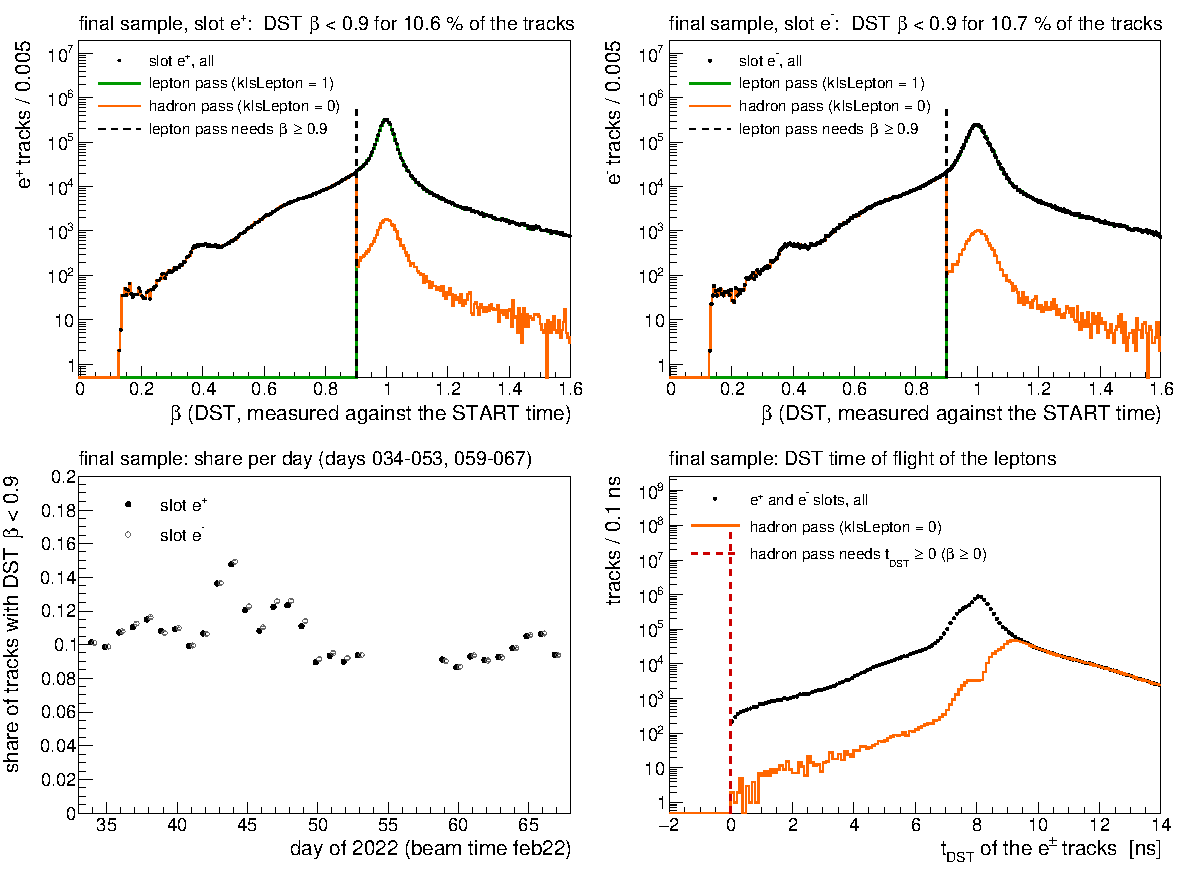
\includegraphics[width=0.95\textwidth]{figs_exp/pid_dstbeta.pdf}
\caption{START-based DST quantities of the leptons of the analysed counts (all combinations, isBest $\ge0$,
$\vz>-500$\,mm, PT3, 29 days). Selection: data, all unlike-sign entries kept by the production in the 29 day files: \ptthreecap{}, a reconstructed event vertex ($\vz>-500$\,mm), particles identified by the START-free velocity \betanew (pions within $3\sigma$, leptons within $5\sigma$ of the expected band; leptons with a RICH ring), all stored combinations (isBest $\ge0$); no corrected-momentum requirement and no target-region cut; the tracks of the $e^+$ and $e^-$ slots. Top: DST $\beta$ of the $e^+$ and $e^-$ slots, split into tracks accepted by
the lepton pass (\code{kIsLepton} $=1$) and by the hadron pass (\code{kIsLepton} $=0$) of the track sorter;
dashed: lepton-pass limit 0.9. Bottom left: share of leptons with DST $\beta<0.9$ per day. Bottom right: DST
time of flight of the leptons near 0; the hadron pass requires tof $\ge0$. In the simulation the share is
0.01--0.03\,\%. Track counts, not normalised to luminosity.}
\label{fig:pid_dstbeta}
\end{figure}

\subsection{Comparison with the earlier LGAD-based production}
\label{sec:oldnew}
The old PAT production used the LGAD START time; the present one uses $\betanew$. Both were processed by
the same FAT configuration and the same fit, with the selection of the first study ($\alab<50^\circ$, no
$\vz>-160$\,mm cut) and with the duplicated entries of the old production removed (\S\ref{sec:dup}).
The new production has 1.38 times more $\eta$-peak content (isBest $\ge0$; 1.44 for isBest $=1$;
Table~\ref{tab:res_oldnew}, Fig.~\ref{fig:oldnew_peak}). The two contents have 8.0\,\% and 8.9\,\% statistical
errors; treated as independent they give $1.38\pm0.17$, an upper bound of the statistical error, because the two
productions share most events (the model spread largely cancels in the ratio of two identical fits and is not
evaluated). Of the new $\eta$ signal, $0.929\pm0.024$ lies in events
with an LGAD start time, the same fraction as for elastic events (0.933): the raw ratio factorises into about
1.07 (events without an LGAD time, a luminosity effect) times about 1.29--1.33 for isBest $\ge0$ (1.35--1.38 for
isBest $=1$; more signal in the same events, a loss of the START-based method of the old production). The simulated $\eta$ processed with both PAT versions
(same DSTs, ideal START) changes only by a factor 1.04 (Fig.~\ref{fig:oldnew_sim}). The LGAD-split numbers
of the table were printed on 2026-11-13 and are not in a saved file (the old compact file is no longer on
disk); the other old/new numbers are confirmed by the saved logs.

% res_oldnew_cnt.tex: copy of res_oldnew.tex with "rows" -> "counts" (analyst, 15 Nov 2026; Part II writer, integ4)
% res_oldnew.tex -- written by hand (numbers: tables_exp/res_oldnew.txt, measured 2026-11-13 with the macros of the old/new comparison)
\begin{table}[H]
\centering\small
\setlength{\tabcolsep}{4pt}
\caption{Old (LGAD start time) against new ($\beta_\mathrm{new}$, relative times) PAT production, the same 29 days, the same FAT configuration and fit.
$\eta$ peak content $S$ from $P_\mathrm{main}$ for $\alpha_\mathrm{lab}<50^\circ$ (no $v_z>-160$~mm cut; selection of the first study).
In the old production the duplicated like-sign entries (52\,\% of the like-sign and 2.7\,\% of the unlike-sign entries) are removed; without this the CB would be 2.1 times too large.
LGAD start: events with evtStart $=1$. The two productions share the DSTs, so the errors of the ratios are not independent and are not quoted.
Last row: SMASH $\eta$ simulation (pure $\eta\to\pi^+\pi^-e^+e^-$ entries) processed with both PAT versions (simulation, ideal START).}
\label{tab:res_oldnew}
\begin{tabular}{lccc}
\toprule
Quantity & old & new & new/old \\
\midrule
$S$, isBest $\geq0$ & $3123\pm278$ & $4319\pm346$ & 1.38 \\
$S$, isBest $=1$ & $2713\pm256$ & $3899\pm311$ & 1.44 \\
$S$, isBest $\geq0$, events with LGAD start & $3023\pm270$ & $4012\pm330$ & 1.33 \\
$S$, isBest $=1$, events with LGAD start & $2629\pm249$ & $3641\pm297$ & 1.38 \\
share of the new $\eta$ signal with LGAD start & -- & $0.929\pm0.024$ & (elastic: 0.933) \\
\midrule
simulation, pure $\eta\to\pi^+\pi^-e^+e^-$ entries, isBest $\geq0$ & 503\,311 & 523\,844 & 1.04 \\
\bottomrule
\end{tabular}
\end{table}


\begin{figure}[H]
\centering
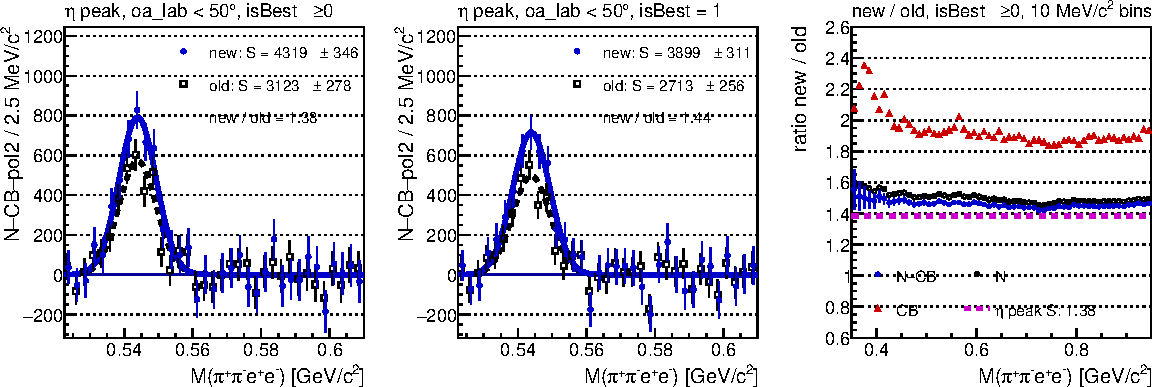
\includegraphics[width=0.85\textwidth]{figs_exp/res_oldnew_peak.pdf}
\caption{The $\eta$ peak in the old (LGAD start time, open squares) and the new ($\betanew$, blue) PAT
production, the same 29 days, selection $\alab<50^\circ$, no $\vz>-160$\,mm cut, corrected momenta, PT3,
$\vz>-500$\,mm. Selection: data of the same 29 days in both productions, with the same cuts: \ptthreecap{}, a reconstructed event vertex ($\vz>-500$\,mm), the particle identification of each production (old: velocity from the LGAD start time; new: START-free \betanew), energy-loss-corrected momenta for all four tracks, angle between the \pipi and the \ee momenta in the laboratory $\alab<50^\circ$, no target-region cut; left all stored combinations (isBest $\ge0$), middle only the best-ranked combination of each event (isBest $=1$); duplicated entries of the old production removed; fit range 0.5225--0.6100\,\GeVcc. Left: $N-\mathrm{CB}-\mathrm{pol2}$ for all combinations (isBest $\ge0$); middle: the same
for isBest $=1$; right: ratio new/old in 10\,\MeVcc bins of $N$ (open circles), CB (red triangles) and
$N-\mathrm{CB}$ (blue); dotted: the $\eta$-peak ratio 1.38. CB $=2\sqrt{N_{++}N_{--}}$, $k=1$; duplicated entries
of the old production removed. Counts, not normalised to luminosity.}
\label{fig:oldnew_peak}
\end{figure}

\begin{figure}[H]
\centering
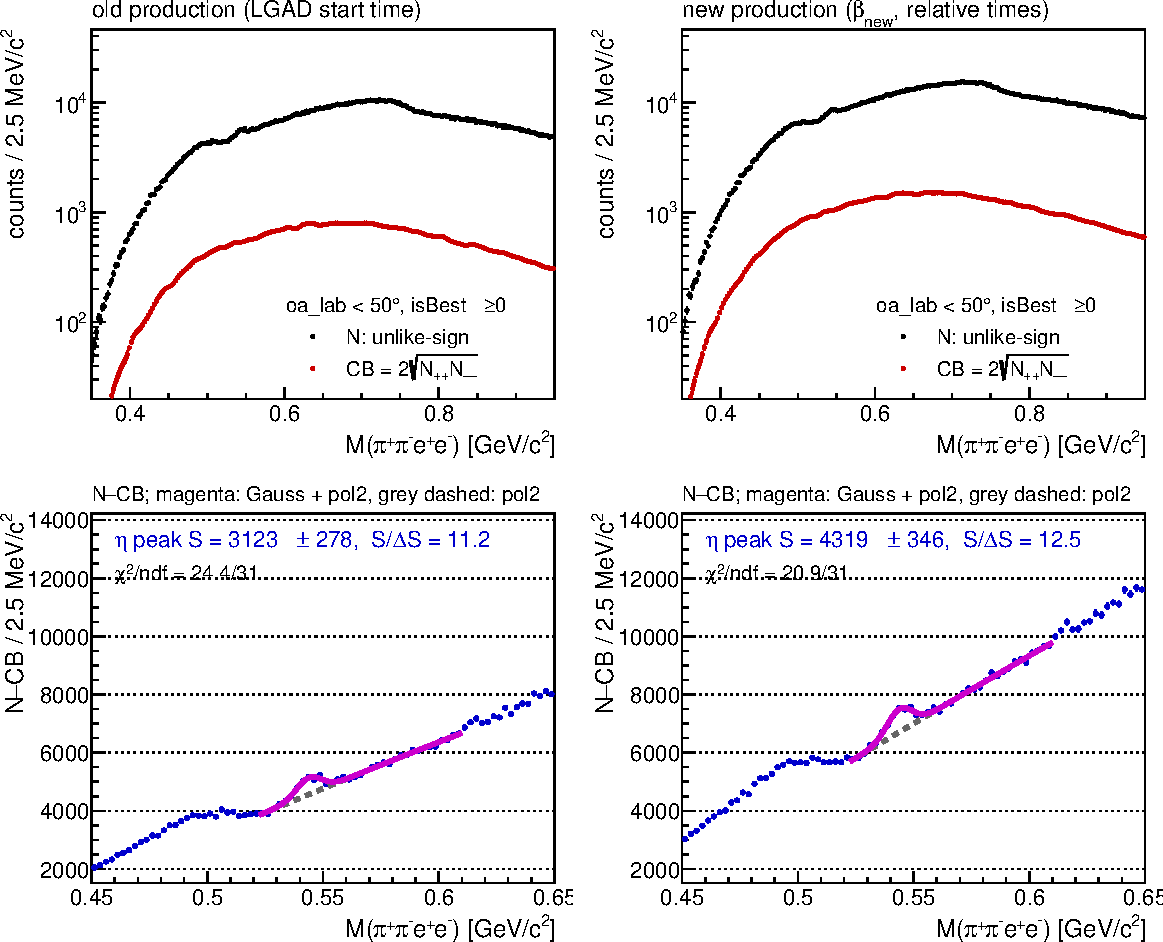
\includegraphics[width=0.76\textwidth]{figs_exp/res_oldnew_spectra_cnt.pdf}
\caption{\Mfour of the old (left) and the new (right) production, $\alab<50^\circ$, all combinations
(isBest $\ge0$), no $\vz>-160$\,mm cut. Selection: data of the same 29 days in both productions, with the same cuts: \ptthreecap{}, a reconstructed event vertex ($\vz>-500$\,mm), the particle identification of each production (old: velocity from the LGAD start time; new: START-free \betanew), energy-loss-corrected momenta for all four tracks, angle between the \pipi and the \ee momenta in the laboratory $\alab<50^\circ$, no target-region cut, all stored combinations (isBest $\ge0$); duplicated entries of the old production removed. Top: $N$ (black) and CB (red), log scale. Bottom: $N-\mathrm{CB}$ with the
\Pmain fit. Counts, not normalised to luminosity.}
\label{fig:oldnew_spectra}
\end{figure}

\begin{figure}[H]
\centering
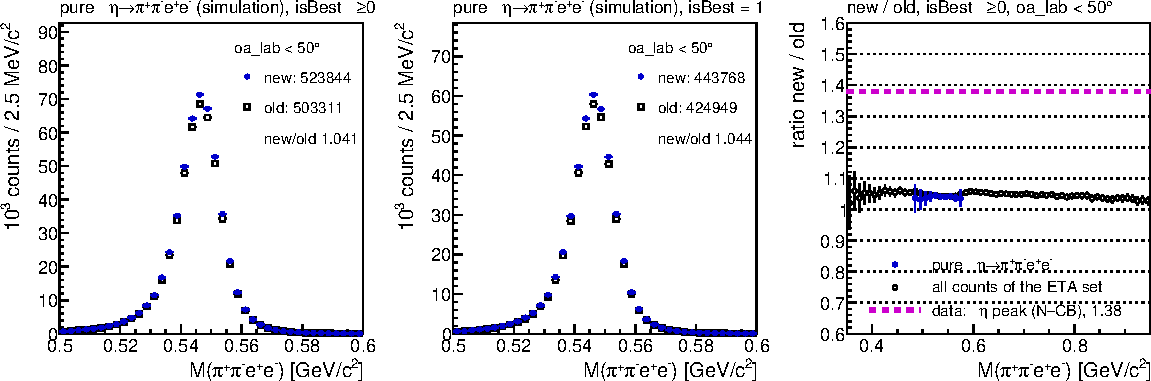
\includegraphics[width=\textwidth]{figs_exp/res_oldnew_sim_cnt.pdf}
\caption{\textbf{Simulation}: the SMASH $\eta$ set processed with both PAT versions (the same DSTs, ideal
START), pure $\eta\to\ppee$ counts, $\alab<50^\circ$. Selection: simulation only (SMASH $\eta$ set, unweighted entries), reconstructed with both PAT versions from the same DSTs and analysed with the simulated PT3 trigger bit, a reconstructed event vertex ($\vz>-500$\,mm) and the angle between the \pipi and the \ee momenta in the laboratory $\alab<50^\circ$, no target-region cut; blue: only true $\eta\to\ppee$ counts (all four tracks from that decay); black: all counts of the $\eta$ set; left all stored combinations (isBest $\ge0$), middle only the best-ranked one (isBest $=1$). Left: isBest $\ge0$; middle: isBest $=1$; right: ratio
new/old for the pure counts (blue, 1.04) and for all counts of the $\eta$ set (black), against the data ratio
1.38 (magenta dashed). Simulated entries (unweighted), no luminosity normalisation; shown only to separate
a data-only loss of the old production from a change of the reconstruction.}
\label{fig:oldnew_sim}
\end{figure}

\subsection{Pion-vertex variables in the compact file}
\label{sec:dzpivar}
The frozen simulation selections use the distance of the pion tracks from the event vertex,
\begin{equation}
\dzpi=\max\left(|z_{\pi^+}-\vz|,\ |z_{\pi^-}-\vz|\right),
\label{eq:dzpi}
\end{equation}
with $z$ the point of a track closest to the beam axis (\code{pip_z}, \code{pim_z}, copied unchanged from
PAT) and $\vz$ = \code{eVertReco_z}, in the same float arithmetic as in the simulation. The first compact file
did not contain these columns. They were added (\code{scan_v2}): the 106 old columns are identical bit by bit
in all three trees, the reference numbers of the first study are reproduced exactly, and no entry has a NaN.
A file without the columns gives NaN, so a \dzpi cut on it selects nothing (easy to spot). On the base
``no $\vz$ cut, $\alab<55^\circ$, $\Mpipi>0.30$'' the new macro reproduces the earlier direct reading from
\code{scan_nt} exactly ($\varepsilon_S=0.968\pm0.036$).

\subsection{Beam energy}
\label{sec:beam}
All kinematics use $T_{\mathrm{beam}}=4530$\,MeV ($\sqrt{s}=3.467$\,GeV). The simulation of Part~I was generated with 4500\,MeV and analysed with
4530\,MeV; this changes \MMfour (and $y_4$) but not \Mfour, \Mee or \Mpipi. The cut $\MMfour<2.85$\,\GeVcc of the
frozen selection PEAK may therefore sit slightly differently in the data. The mass scales of the data are
in \S\ref{sec:scale}.

%======================================================================
\section{File locations and commands}
\label{app:files}
%======================================================================
\textbf{Files.} $P$ $=$ \code{/hdd3/przygoda/HADES/FAT_out/exp/pippimepem_isBestAll_T4530}, $R$ $=$ the repository
\code{/home/przygoda/HADES/FAT/FAT} (branch \code{pp45_pippimepem}).

{\small
\begin{tabularx}{\textwidth}{@{}>{\raggedright\arraybackslash}p{3.6cm} L@{}}
\toprule
PAT input & \code{/hdd3/przygoda/HADES/files/exp/gen4/lep_<day>.root}, list \code{lep_betanew.list} (29 files) \\
PID cut file & \code{pp45_pid_cuts_exp_betanew_v1.root} (PAT repository; copy in \code{$P/report_exp/pid/inputs/}) \\
FAT outputs & \code{$P/output_pippim{epem,epep,emem}_exp.root}, production log \code{$P/production.log} \\
Compact file & \code{$P/scan_v2/scan_compact.root} (with the pion-vertex variables); first version \code{$P/scan/scan_compact.root} \\
First scan study & \code{$P/scan/*.txt}, figures \code{$R/plots/output/eta_scan/} \\
Luminosity inputs & \code{$P/report_exp/smp/lumi_inputs/*.csv} (revision N: per run, per day, per period, coverage of the data) \\
Report macros & \code{$R/plots/exp_report/{prep,smp,pid,spec,cb,opt,res}_*.C} (+ \code{*_common.h}); verification macros \code{verify_*.C} \\
Event-vertex study & macros \code{$R/plots/all_report/vtx_*.C}, \code{vtx_*.h}, \code{vtx_numbers.py} (copies of the verifier's code, \S\ref{sec:vtxeff}); final review: \code{fix2_vtx_fig.C} (figure), \code{fix2_numbers.py} ($E\times1.2$, combinations); entry dumps and outputs \code{/hdd3/przygoda/HADES/FAT_out/vtx_eff/ve_verify/}; results \code{$R/docs/latex/tables_all/vtx_*.txt}; notes \code{$R/docs/latex/notes_all/ve_*_note.md} \\
Target walls (Part~III, WP2) & empty-target PAT, FAT and compact files \code{/hdd3/przygoda/HADES/FAT_out/all_report/wp2/empty/{pat,fat2,scan2}} (\code{scan2/scan_compact_empty.root}); macros \code{$R/plots/all_report/wp2_*.C}, \code{wp2_*.py}; tables \code{$R/docs/latex/tables_all/wp2_*.txt}; figures \code{$R/docs/latex/figs_all/wp2_N1v2.pdf}, \code{vw2a_fig.pdf}; notes \code{$R/docs/latex/notes_all/wp2_results.md} (section 7: verification and decision) and \code{$R/docs/latex/notes_all/verify_wp2/} \\
Bootstrap of $E$ (Part~III) & package bedge with its verifier vbedge: \code{report_all.pdf} (section on the bump edge, ``Statistical and MC errors''), \code{$R/docs/latex/tables_all/bedge_results.txt} \\
Halo check of the rate steps & per-day rates \code{$R/docs/latex/tables_exp/smp_rates_perday.txt}; per-day halo levels of the verifier vw2b (\code{out_e.txt}, \code{out_g.txt}) \\
Engine & \code{$R/plots/ScanEngine.h}, \code{$R/plots/scan_prepare.C} \\
Intermediate files & \code{$P/report_exp/<prefix>/} (ROOT files, run logs), ACLiC builds \code{$P/report_exp/aclic_<prefix>/} \\
Figures, tables & \code{$R/docs/latex/figs_exp/*.pdf} (+ PNG previews), \code{$R/docs/latex/tables_exp/*.tex}, \code{*.txt} (all numbers) \\
This report & \code{$R/docs/latex/report_exp.tex}, \code{report_exp_short.tex} \\
\bottomrule
\end{tabularx}
}

\textbf{Commands} (a bash session in \fpath{/home/przygoda/HADES/FAT/FAT}; the lines that need another directory run in a
subshell, so the working directory stays the repository). Every macro is compiled with ACLiC into a build directory outside the
repository; below, \code{<B x>} stands for the ROOT expression
\begin{lstlisting}
gSystem->SetBuildDir("/hdd3/przygoda/HADES/FAT_out/exp/pippimepem_isBestAll_T4530/report_exp/aclic_x", kTRUE)
\end{lstlisting}
written out in full in each command, and the first line defines the production directory \code{$P}.
\begin{lstlisting}
P=/hdd3/przygoda/HADES/FAT_out/exp/pippimepem_isBestAll_T4530
cd /home/przygoda/HADES/FAT/FAT
# compact file with the pion-vertex variables (60 s) and the reference numbers (10 s)
root -l -b -q -e '<B prep>' 'plots/scan_prepare.C+'
root -l -b -q -e '<B prep>' 'plots/scan_reference.C+'
root -l -b -q -e '<B prep>' 'plots/exp_report/prep_dzpi.C+'           # dz_pi check
# samples, luminosity, cut flow, rates, sectors, peak per period
mkdir -p $P/report_exp/smp/lumi_inputs   # then copy the four luminosity CSV files (revision N)
root -l -b -q -e '<B smp>' 'plots/exp_report/smp_pat_counts.C+(53)'    # compile once
for d in 34 35 36 37 38 39 40 41 42 43 44 45 46 47 48 49 50 51 52 53 59 60 61 62 63 64 65 66 67; do echo $d; done | \
  xargs -P 6 -I{} root -l -b -q -e '<B smp>' 'plots/exp_report/smp_pat_counts.C+({})'
root -l -b -q -e '<B smp>' 'plots/exp_report/smp_flow.C+'
root -l -b -q -e '<B smp>' 'plots/exp_report/smp_report.C+'
# PID (final sample 29 days, 6 parallel jobs), figures, signal by DST beta, simulation START check
bash plots/exp_report/pid_run_final.sh
( cd $P/report_exp/pid && root -l -b -q -e '<B pid>' '/home/przygoda/HADES/FAT/FAT/plots/exp_report/pid_draw.C+' )
( cd /home/przygoda/HADES/FAT/FAT/plots && root -l -b -q -e '<B pid>' 'exp_report/pid_peak_dstbeta.C+' )
root -l -b -q -e '<B pid>' '/home/przygoda/HADES/FAT/FAT/plots/exp_report/pid_sim_startcheck.C+'
# spectra and kinematics; FAT vertex cut on the PAT input
root -l -b -q -e '<B spec>' 'plots/exp_report/spec_m4.C+'
root -l -b -q -e '<B spec>' 'plots/exp_report/spec_vars.C+'
root -l -b -q -e '<B spec>' 'plots/exp_report/spec_vz500.C+("fill",0,1)'
root -l -b -q -e '<B spec>' 'plots/exp_report/spec_vz500.C+("draw")'
# combinatorial background: event mixing first, then the checks
root -l -b -q -e '<B cb>' 'plots/exp_report/cb_kmix.C+'
root -l -b -q -e '<B cb>' 'plots/exp_report/cb_checks.C+'
# optimisation: sculpting first (opt_scans reads its flags)
root -l -b -q -e '<B opt>' 'plots/exp_report/opt_sculpt.C+'
root -l -b -q -e '<B opt>' 'plots/exp_report/opt_scans.C+'
root -l -b -q -e '<B opt>' 'plots/exp_report/opt_named.C+'
root -l -b -q -e '<B opt>' 'plots/exp_report/opt_bias.C+'
# results (copy lumi_coverage_perrun.csv to $P/report_exp/res/ first)
root -l -b -q -e '<B res>' 'plots/exp_report/res_peak.C+'
root -l -b -q -e '<B res>' 'plots/exp_report/res_bump.C+'
root -l -b -q -e '<B res>' 'plots/exp_report/res_mee.C+'
# review fixes: model uncertainty, error calibration, displaced positions, side bands, MM4 efficiency
root -l -b -q -e '<B fix>' 'plots/exp_report/fix_checks.C+'
# eta efficiency of the event-vertex cut (after the review; the commands of every vtx_* macro are in its header)
V='gSystem->SetBuildDir("/hdd3/przygoda/HADES/FAT_out/vtx_eff/ve_verify/aclic", kTRUE)'
seq 0 28 | xargs -P 6 -I{} sh -c "root -l -b -q -e '$V' 'plots/all_report/vtx_fill.C+({},0)'"   # entries from the PAT files
for m in vtx_ana vtx_ana2 vtx_ana3; do root -l -b -q -e "$V" "plots/all_report/$m.C+"; done
python3 -I plots/all_report/vtx_numbers.py
root -l -b -q -e 'gSystem->SetBuildDir("/hdd3/przygoda/HADES/FAT_out/vtx_eff/ve_verify/aclic_fig", kTRUE)' 'plots/all_report/vtx_fig.C+'
# this report
( cd docs/latex && pdflatex report_exp && pdflatex report_exp )
\end{lstlisting}

The old/new comparison figures (\code{res_oldnew_*}) and Table~\ref{tab:res_oldnew} come from the study of 2026-11-13 (copied and
cropped, numbers written by hand from its logs). The independent verifications are run by the macros
\code{plots/exp_report/verify_{smp,pid,spec,cb,opt,res}_*.C}; their outputs are in \code{$P/report_exp/<prefix>/verify/} or
\code{$P/report_exp/<prefix>_verify/}. The table \code{tables_exp/wr_res_period_cnt.tex} is a copy of \code{res_period.tex} with one
caption reference adapted for this report; \code{tables_exp/wr_res_bump_cnt.tex} is a copy of \code{res_bump.tex} whose caption sentence on the
statistical errors was updated for the bootstrap (numbers unchanged). The figures \code{figs_exp/<name>_cnt.pdf} (and
\code{figs_all/<name>_cnt.pdf}) are redrawn by copies of their macros with the same suffix (\code{plots/exp_report/}, \code{plots/all_report/}; for \code{spec_m4_overview}, \code{spec_m4_isbest} and \code{spec_vertexcut} the copy \code{spec_m4_cnt2.C}),
on the same inputs; only the word ``rows'' in their labels became ``counts''.

\end{document}
